\documentclass[nohyper,nobib]{tufte-book}
\usepackage{nameref}
% \hypersetup{colorlinks}
\usepackage{hyphenat}
\usepackage{url}
\usepackage{amssymb}
\usepackage{amsmath}
% \usepackage[backend=biber, natbib=true, style=numeric]{biblatex}
% \addbibresource{main.bib}
\usepackage{xargs}
% \renewcommandx{\cite}[3][1={0pt},2={}]{\sidenote[][#1]{\fullcite[#2]{#3}}}
\usepackage[slovene]{babel}
\usepackage{datetime}
\newcommand{\monthyear}{%
  \ifcase\month
  \or januar%
  \or februar%
  \or marec%
  \or april%
  \or maj%
  \or junij%
  \or julij%
  \or avgust%
  \or september%
  \or oktober%
  \or november%
  \or december%
  \fi
  \space\number\year
}
\newcommand{\runinheading}[1]{%
  \vspace*{5mm}%
  \noindent\textbf{#1}.%
}

\title{Uvod v odkrivanje znanj iz podatkov}
\date{2026}
\author[Blaž Zupan]{Blaž Zupan}
\publisher{Univerza v Ljubljani}

%%
% If they're installed, use Bergamo and Chantilly from www.fontsite.com.
% They're clones of Bembo and Gill Sans, respectively.
%\IfFileExists{bergamo.sty}{\usepackage[osf]{bergamo}}{}% Bembo
%\IfFileExists{chantill.sty}{\usepackage{chantill}}{}% Gill Sans

\usepackage{booktabs} % For nicely typeset tabular material

\usepackage{graphicx}
\setkeys{Gin}{width=\linewidth,totalheight=\textheight,keepaspectratio}
\graphicspath{{graphics/}}

% The fancyvrb package lets us customize the formatting of verbatim
% environments.  We use a slightly smaller font.
\usepackage{fancyvrb}
\fvset{fontsize=\normalsize}

% Prints argument within hanging parentheses (i.e., parentheses that take
% up no horizontal space).  Useful in tabular environments.
\newcommand{\hangp}[1]{\makebox[0pt][r]{(}#1\makebox[0pt][l]{)}}

% Prints an asterisk that takes up no horizontal space.
% Useful in tabular environments.
\newcommand{\hangstar}{\makebox[0pt][l]{*}}

% Prints a trailing space in a smart way.
\usepackage{xspace}


% Prints an epigraph and speaker in sans serif, all-caps type.
\newcommand{\openepigraph}[2]{%
  %\sffamily\fontsize{14}{16}\selectfont
  \begin{fullwidth}
  \sffamily\large
  \begin{doublespace}
  \noindent\allcaps{#1}\\% epigraph
  \noindent\allcaps{#2}% author
  \end{doublespace}
  \end{fullwidth}
}

% Inserts a blank page
\newcommand{\blankpage}{\newpage\hbox{}\thispagestyle{empty}\newpage}

% Excercise box
\usepackage{mdframed}
\usepackage{needspace}
\usepackage{xcolor}
\definecolor{exerciseblue}{RGB}{40,90,150}

\newenvironment{exercise}[1]
{
\Needspace{8\baselineskip}
\begin{mdframed}[
  linewidth=1.1pt,
  linecolor=exerciseblue,
  topline=true,
  leftline=true,
  rightline=false,
  bottomline=false,
  userdefinedwidth=0.98\linewidth,
  leftmargin=0pt,
  rightmargin=0pt,
  innerleftmargin=0.8em,
  innerrightmargin=0.8em,
  innertopmargin=0.6em,
  innerbottommargin=0.4em,
  skipabove=1em,
  skipbelow=1em
]
\small
\noindent\textsc{Poskusi sam: #1}\par
\vspace{0.7em}
\noindent\ignorespaces
}
{
\end{mdframed}
}

% \usepackage{units}

% Typesets the font size, leading, and measure in the form of 10/12x26 pc.
\newcommand{\measure}[3]{#1/#2$\times$\unit[#3]{pc}}

% Macros for typesetting the documentation
\newcommand{\hlred}[1]{\textcolor{Maroon}{#1}}% prints in red
\newcommand{\hangleft}[1]{\makebox[0pt][r]{#1}}
\newcommand{\hairsp}{\hspace{1pt}}% hair space
\newcommand{\hquad}{\hskip0.5em\relax}% half quad space
\newcommand{\TODO}{\textcolor{red}{\bf TODO!}\xspace}
\newcommand{\ie}{\textit{i.\hairsp{}e.}\xspace}
\newcommand{\eg}{\textit{e.\hairsp{}g.}\xspace}
\newcommand{\na}{\quad--}% used in tables for N/A cells
\providecommand{\XeLaTeX}{X\lower.5ex\hbox{\kern-0.15em\reflectbox{E}}\kern-0.1em\LaTeX}
\newcommand{\tXeLaTeX}{\XeLaTeX\index{XeLaTeX@\protect\XeLaTeX}}
% \index{\texttt{\textbackslash xyz}@\hangleft{\texttt{\textbackslash}}\texttt{xyz}}
\newcommand{\tuftebs}{\symbol{'134}}% a backslash in tt type in OT1/T1
\newcommand{\doccmdnoindex}[2][]{\texttt{\tuftebs#2}}% command name -- adds backslash automatically (and doesn't add cmd to the index)
\newcommand{\doccmddef}[2][]{%
  \hlred{\texttt{\tuftebs#2}}\label{cmd:#2}%
  \ifthenelse{\isempty{#1}}%
    {% add the command to the index
      \index{#2 command@\protect\hangleft{\texttt{\tuftebs}}\texttt{#2}}% command name
    }%
    {% add the command and package to the index
      \index{#2 command@\protect\hangleft{\texttt{\tuftebs}}\texttt{#2} (\texttt{#1} package)}% command name
      \index{#1 package@\texttt{#1} package}\index{packages!#1@\texttt{#1}}% package name
    }%
}% command name -- adds backslash automatically
\newcommand{\doccmd}[2][]{%
  \texttt{\tuftebs#2}%
  \ifthenelse{\isempty{#1}}%
    {% add the command to the index
      \index{#2 command@\protect\hangleft{\texttt{\tuftebs}}\texttt{#2}}% command name
    }%
    {% add the command and package to the index
      \index{#2 command@\protect\hangleft{\texttt{\tuftebs}}\texttt{#2} (\texttt{#1} package)}% command name
      \index{#1 package@\texttt{#1} package}\index{packages!#1@\texttt{#1}}% package name
    }%
}% command name -- adds backslash automatically
\newcommand{\docopt}[1]{\ensuremath{\langle}\textrm{\textit{#1}}\ensuremath{\rangle}}% optional command argument
\newcommand{\docarg}[1]{\textrm{\textit{#1}}}% (required) command argument
\newenvironment{docspec}{\begin{quotation}\ttfamily\parskip0pt\parindent0pt\ignorespaces}{\end{quotation}}% command specification environment
\newcommand{\docenv}[1]{\texttt{#1}\index{#1 environment@\texttt{#1} environment}\index{environments!#1@\texttt{#1}}}% environment name
\newcommand{\docenvdef}[1]{\hlred{\texttt{#1}}\label{env:#1}\index{#1 environment@\texttt{#1} environment}\index{environments!#1@\texttt{#1}}}% environment name
\newcommand{\docpkg}[1]{\texttt{#1}\index{#1 package@\texttt{#1} package}\index{packages!#1@\texttt{#1}}}% package name
\newcommand{\doccls}[1]{\texttt{#1}}% document class name
\newcommand{\docclsopt}[1]{\texttt{#1}\index{#1 class option@\texttt{#1} class option}\index{class options!#1@\texttt{#1}}}% document class option name
\newcommand{\docclsoptdef}[1]{\hlred{\texttt{#1}}\label{clsopt:#1}\index{#1 class option@\texttt{#1} class option}\index{class options!#1@\texttt{#1}}}% document class option name defined
\newcommand{\docmsg}[2]{\bigskip\begin{fullwidth}\noindent\ttfamily#1\end{fullwidth}\medskip\par\noindent#2}
\newcommand{\docfilehook}[2]{\texttt{#1}\index{file hooks!#2}\index{#1@\texttt{#1}}}
\newcommand{\doccounter}[1]{\texttt{#1}\index{#1 counter@\texttt{#1} counter}}

% Generates the index
% \usepackage{makeidx}
% \makeindex
% Define \index as no-op if makeidx is not used
\providecommand{\index}[1]{}

%%%% Kevin Godny's code for title page and contents from https://groups.google.com/forum/#!topic/tufte-latex/ujdzrktC1BQ
\makeatletter
\renewcommand{\maketitlepage}{%
\begingroup%
\setlength{\parindent}{0pt}

{\fontsize{24}{24}\selectfont\textit{\@author}\par}

\vspace{1.75in}{\fontsize{36}{54}\selectfont\@title\par}

\vspace{0.5in}{\fontsize{14}{14}\selectfont\textsf{\smallcaps{\@date}}\par}

\vfill{\fontsize{14}{14}\selectfont\textit{\@publisher}\par}

\thispagestyle{empty}
\endgroup
}
\makeatother

\titlecontents{part}%
    [0pt]% distance from left margin
    {\addvspace{0.25\baselineskip}}% above (global formatting of entry)
    {\allcaps{Part~\thecontentslabel}\allcaps}% before w/ label (label = ``Part I'')
    {\allcaps{Part~\thecontentslabel}\allcaps}% before w/o label
    {}% filler and page (leaders and page num)
    [\vspace*{0.5\baselineskip}]% after

\titlecontents{chapter}%
    [4em]% distance from left margin
    {}% above (global formatting of entry)
    {\contentslabel{2em}\textit}% before w/ label (label = ``Chapter 1'')
    {\hspace{0em}\textit}% before w/o label
    {\qquad\thecontentspage}% filler and page (leaders and page num)
    [\vspace*{0.5\baselineskip}]% after
%%%% End additional code by Kevin Godby
\usepackage{siunitx}

\usepackage{listings}
\usepackage{listingsutf8}
\lstset{
    language=Python,
    basicstyle=\ttfamily\small,          % Code font style
    keywordstyle=\color{blue}\bfseries,  % Keywords in blue
    commentstyle=\color{gray},           % Comments in gray
    stringstyle=\color{red},             % Strings in red
    frame=lines,                         % Adds frame around the code
    numbers=none,                        % No line numbers
    showstringspaces=false,              % Don't show spaces in strings
    backgroundcolor=\color{white},       % White background (default)
    inputencoding=utf8,
    extendedchars=true,
    literate=
        {č}{{\v c}}1
        {ć}{{\'c}}1
        {đ}{{\dj}}1
        {š}{{\v s}}1
        {ž}{{\v z}}1
        {Č}{{\v C}}1
        {Ć}{{\'C}}1
        {Đ}{{\DJ}}1
        {Š}{{\v S}}1
        {Ž}{{\v Z}}1
        {∂}{{$\partial$}}1
}

\usepackage{multirow}
\usepackage{array}
\usepackage{tabularx}
\usepackage{makecell}
\usepackage{siunitx}
\usepackage{hyperref}

% Allow flexible page heights to avoid underfull vbox warnings
\raggedbottom

\renewcommand{\tablename}{Tabela}
\renewcommand{\figurename}{Slika}

\begin{document}

% Front matter
\frontmatter

% r.3 full title page
\maketitle


% v.4 copyright page
\newpage
\begin{fullwidth}
~\vfill
\thispagestyle{empty}
\setlength{\parindent}{0pt}
\setlength{\parskip}{\baselineskip}
Copyright \copyright\ \the\year\ \thanklessauthor

\par\smallcaps{Študijsko gradivo, \thanklesspublisher}

\par To delo je izdano pod licenco Priznanje avtorstva-Nekomercialno-Deljenje pod enakimi pogoji 4.0 Mednarodna (CC BY-NC-ND 4.0). Delo je prosto dostopno na spletnih straneh predmeta Odkrivanje znanj iz podatkov, ki se izvaja na UL FRI.

\par\textit{Delovno verzija, \monthyear}
\end{fullwidth}

% r.5 contents
\tableofcontents


% r.9 introduction
\cleardoublepage
\chapter*{Uvod}

Pričujoči zapiski nastajajo v okviru predavanj pri predmetu Uvod v odkrivanje znanj iz podatkov. Predmet izvajamo že dolgo, morda že 20 let, in se je od svojega nastanka precej spreminjal. Njegovo čudno ime izvira iz poimenovanja področja podatkovnih znanosti na prelomu stoletja, ki je hotelo izpostaviti, da lahko iz industrijskih in znanstvenih baz podatkov odkrijemo novo znanje in ga s pridom uporabimo. Angleški izraz {\em knowledge discovery in databases} se je takrat uporabljal vzporedno z izrazom {\em data mining}, podatkovno rudarjenje, morda tudi zato, da bi nadomestil takrat manj popularen izraz strojno učenje. Predmet strojno učenje je bil na UL FRI sicer od nekdaj, in zaradi želje po predmetu, ki bi se osredotočil na razumevanje podatkov, ni bilo drugega, kot privzeti malce drugačno poimenovanje.

Predmet se je po vsebini z leti zelo spremenil. Sprva je bil izvajan v prvem semestru tretjega letnika in je imel priložnost sistematičnega obravnavanja pristopov razložljivega strojnega učenja. Po prestavitvi v drugi semester pa je tu moral zavzeti popolnoma drugačno vlogo, saj so študenti pri predhodnih predmetih slišali, sicer mnogokrat precej na hitro, praktično o vseh pristopih, ki se danes uporabljajo v strojnem učenju. Predmet zato krmilimo v dve smeri: poglobljeno praktično razumevanje področja, od samih osnov naprej, in poudarek na tehnikah, ki osvetlijo podatke z razložljivimi modeli, ki jih lahko uporabniki pojasnijo in z njimi odkrijejo vzorce v podatkih ter morda na ta način razložijo procese, ki so podatke generirali.

Velik vpliv na sestavo predmeta imajo izobraževalni videi Andreja Karpathya, predvsem njegov pristop, kjer sicer kompleksne koncepte razloži z razvojem programov, iz nule, v Pythonu. Ta pristop uporabljamo tudi pri predmetu, zato je v zapiskih veliko kode. Snov podajamo tudi z enačbami in razlagami, a sledimo temu, da je prav vse potem zapisano v programih. Znanje algoritmičnega razmišljanja in zapisa postopkov v kodi je osnova računalniškega inženirstva.

\mainmatter

%\part{Part Name}
\chapter{Gradientni sestop, odvajanje in računski graf}

Večina postopkov, ki jih bomo spoznali in uporabljali pri predmetu o ``odkrivanje znanj iz podatkov'' temelji na modernih pristopih strojnega učenja. Ta, poenostavljeno, gradi modele iz učnih podatkov tako, da pri določeni podani strukturi modela išče njegove parametre tako, da pri tem zadovolji pogoje kriterijske funkcije, ki jo določimo nad učnimi podatki. Zadovoljevanje pogojev tipično pomeni minimizacijo kriterijske funkcije in s tem uporabo optimizacijskih algoritmov. Iz zgrajenih modelov razpoznamo vzorce v podatkih in če so ti razumljivo zapisani ali pa jasno izrisani v nekem grafičnem prikazu lahko modele, in s tem podatke, interpretiramo in iz interpretacij morda odkrijemo nova znanja.

Zgornji odstavek je začetek prvega poglavja nekega predmeta precej preobložen. Do njegovega razumevanja se bomo morali še prebiti. A to ne bomo počeli v tem poglavju. Prejšnji odstavek smo namreč zapisali samo zato, da uvedem pojem ``kriterijske funkcije'' in namignemo, da za neko, lahko enostavno lahko pa zelo kompleksno funkcijo, iščemo njen ``minimum''. Tu se zaenkrat ustavimo in si vse skupaj poglejmo na enostavnem primeru.

\section{Primer}

Začnimo s preprosto funkcijo: 

\[
f(a) = a^2 - 10a + 28
\]

\noindent Želimo poiskali takšno vrednost parametra \( a \), pri kateri ima ta funkcija najnižjo vrednost.

\textbf{Analitična rešitev}. Ker je dana funkcija enostavna, kvadratna, lahko njen minimum poiščemo analitično. Funkcija bo imela ekstrem v točki, kjer je prvi odvod enak nič. Odvajamo našo funkcijo:  

\[
\frac{d}{da} f(a) = 2a - 10
\]

\noindent in njen odvod enačimo z nič:  

\[
2a - 10 = 0
\]

\noindent Rešimo za \( a \):  

\[
a = 5
\]

\noindent Vrednost funkcije v tej točki je:  

\[
f(5) = 5^2 - 10(5) + 28 = 25 - 50 + 28 = 3
\]

\noindent Torej funkcija doseže svoj minimum pri \( a = 5 \), kjer velja \( f(5) = 3 \).  

\textbf{Numerična rešitev}. Poiščimo to rešitev še numerično. Postopek iskanja minimuma bomo pričeli pri neki izbrani vrednosti parametra \( a \), tam izračunali odvod funkcij, in vrednost parametra spremenili v smeri negativnega odvoda, torej $a$ povečali, če bo odvod negativen, ali pa $a$ zmanjšali, če bo odvod pozitiven. 

Razmislimo: pri pozitivnem odvodu funkcije za izbrano vredno parametra $a$ se pri povečanju te vrednosti $a$ vrednost funkcije zveča. Odvod nam namreč pove v katero smer in kako hitro se vrednost funkcije spremeni pri majhni spremembi parametra 
$a$. Zato, če iščemo minimum, moramo vrednost $a$ zmanjšati. Odločiti se moramo seveda za koliko jo bomo zmanjšali, a intuitivno je to prav gotovo odvisno od velikosti odvoda: če pri vrednosti $a$ funkcija hitro narašča, torej je odvod visok, lahko vrednost $a$ popravimo za več kot v primeru, ko je naraščanje zelo počasno in smo morda že prav blizu ekstrema funkcije. Podobno, samo z ravno nasprotnim predznakom, lahko ravnamo ob negativnem odvodu, popravek parametra $a$ pa lahko zapišemo z:
\[
a_{t+1} = a_t - \eta \frac{d}{da} f(a_t)
\]
\noindent kjer je $a_{t+1}$ vrednost parametra po $t$-tem popravku in kjer je $\eta$ korak popravka, v strojnem učenju pa ga bomo imenovali tudi {\em hitrost učenja}. Meta parameter $\eta$ torej določa, kako veliki bodo koraki pri posodabljanju vrednosti parametra. Imenujemo ga {\em meta} ker je parameter naše numerične metode, s katero iščemo rešitev, in torej ne parameter funkcije, ki jo optimiziramo (tem parametrom pravimo samo parameteri, brez predpone ``meta'').

Vse skupaj seveda pričnemo pri neki {\em začetni vrednosti} parametra, $a_0$. Na primer, začnimo z začetno vrednostjo $a_0=6$ in izberimo hitrost učenja $\eta = 0.1$ ter poglejmo, kam vse skupaj vodi:

\begin{enumerate}
\item Izračunamo odvod funkcije pri \( a_0 = 6 \):
\[
\frac{d}{da} f(6) = 2(6) - 10 = 12 - 10 = 2
\]
\noindent in posodobimo vrednost parametra,
\[
a_1 = 6 - 0.1 \times 2 = 6 - 0.2 = 5.8
\]
\item Izračunamo odvod pri novi vrednosti parametra, \( a_1 = 5.8 \):
\[
\frac{d}{da} f(5.8) = 2(5.8) - 10 = 11.6 - 10 = 1.6
\]
\noindent in ponovno posodobimo njegovo vrednost,
\[
a_2 = 5.8 - 0.1 \times 1.6 = 5.8 - 0.16 = 5.64
\]
\item Izračunamo gradient pri \( a_2 = 5.64 \):
\[
\frac{d}{da} f(5.64) = 2(5.64) - 10 = 11.28 - 10 = 1.28
\]
\noindent in posodobimo vrednost parametra $a$, 
\[
a_3 = 5.64 - 0.1 \times 1.28 = 5.64 - 0.128 = 5.512
\]
\end{enumerate}

Smo opazili, da se vrednost odvoda funkcije zmanjšuje, z njo pa tudi zmanjšujejo spremembe parametra $a$? Postopek bi morali seveda nadaljevati, in če je vse tako, kot smo si zamislili, bi se morala vrednost parametra $a$ približati 5. Tam gre tudi odvod funkcije $f(a)$ proti nič in z njo gredo proti nič tudi vrednost popravkov parametra.

Čas je, da tovrstno iskanje minimuma funkcije implementiramo v kodi:

\vspace*{3mm}
\begin{lstlisting}
def f(a):
    return a**2 - 10*a + 28

def df(a):
    return 2*a - 10

a = 6
eta = 0.1
for _ in range(20):
    grad = df(a)
    a = a - eta * grad
    print(f"a = {a:.6f}, f(a) = {f(a):.6f}")
\end{lstlisting}

Pomagali smo si z analitičnim odvodom funkcije, in ga zapisali v funkciji \texttt{df}. Ko program poženemo, se ta hitro približa pravi rešitvi:

\vspace*{3mm}
\begin{lstlisting}
a = 5.800000, f(a) = 3.640000
a = 5.640000, f(a) = 3.409600
a = 5.512000, f(a) = 3.262144
...
a = 5.014412, f(a) = 3.000208
a = 5.011529, f(a) = 3.000133
\end{lstlisting}

Namesto analitičnega zapisa odvoda funkcije lahko tega izračunamo tudi numerično z metodo končnih diferenc, kot smo to storili v spodnji funkciji.
\vspace*{3mm}
\begin{lstlisting}
def df(a, h=0.0001):
    return (f(a + h) - f(a)) / h
\end{lstlisting}

\noindent Tipično je uporaba analitično izračunanega odvoda oziroma gradientov hitrejša in bolj točna ter ni odvisna od uporabe parametra \texttt{h}, katerega vrednost bi morali še določiti (zgoraj smo sicer izbrali privzeto vrednost 0.0001) in ki dejansko vpliva na točnost rezultatov. Zato se bomo od tu dalje delali z analitično izračunanimi odvodi!

\section{Gradientni sestop}

Preden nadaljujemo z (analitičnim) odvajanjem samo zabeležimo in poimenujmo: postopek, ki smo ga zgoraj uporabili za izračun minimuma dane funkcije, se imenuje {\em gradientni sestop}. Ta v vsakem koraku oceni, kako strma je funkcija pri dani vrednosti parametra in nato njegovo vrednost popravi v smeri negativnega odvoda. Pomembno je izbrati ustreen korak popravka $\eta$. Če je prevelika, se nam lahko zgodi, da bomo minimum ``preskočili'', če je premajhna, bo postopek zelo počasen.

Da lahko izvedemo gradientni sestop, moramo poznati odvod funkcije po danem parametru. 
V primeru enega parametra je gradient enak navadnemu odvodu, 
v primeru večparametrske funkcije pa moramo poznati odvode po vseh parametrih. 
Vektorju teh odvodov pravimo gradient in ga označimo z $\nabla f(\boldsymbol{\theta})$, 
kjer je $\boldsymbol{\theta}$ vektor parametrov:

\[
\nabla f(\boldsymbol{\theta}) = 
\left(
\frac{\partial f}{\partial \theta_1},
\frac{\partial f}{\partial \theta_2},
\dots,
\frac{\partial f}{\partial \theta_n}
\right)^T
\]

Tudi gradient funkcije lahko določimo analitično ali numerično z metodo končnih diferenc, a bomo, zaradi enakih razlogov kot pri odvajanju, tudi tu uorabili analitično rešitev. Ker je ročno odvajanje za kompleksne funkcije (beri: kompleksne modele), kot so na primer nevronske mreže, zamudno, se moramo zateči k boljši rešitvi: uporabi programa za odvajanje. Program za strojno odvajanje bomo razvili v naslednjem poglavju, tu pa si poglejmo, kako se problema strojnega odvajanja sploh lotimo, najprej torej ročno.


\section{Računski graf}

Začnimo s primerom in z enostavno funkcijo štirih parametrov:

\[
L(a, b, c, d) = (ab + c) d
\]

Za to funkcijo bi radi izračunali gradient pri vrednostih njenih parametrov \( a = 2 \), \( b = -3 \), \( c = 10 \), \( d = -2 \). Želeli bi torej izračunati sledeče parcialne odvode:
%
\[
\frac{\partial L}{\partial a}, \frac{\partial L}{\partial b}, \frac{\partial L}{\partial c}, \frac{\partial L}{\partial d}.
\]
%
\noindent Z drugimi besedami, želeli bi izračunati gradient funkcije pri danih vrednosti parametrov:
\[
\nabla L = \left( \frac{\partial L}{\partial a}, \frac{\partial L}{\partial b}, \frac{\partial L}{\partial c}, \frac{\partial L}{\partial d} \right)
\]

Najprej si skušajmo olajšati naše računanje odvodov tako, da funkcijo razstavimo in zapišemo z vpeljavo vmesnih spremenljivk, katerih vrednost izračunamo z neko osnovno operacijo (množenje ali seštevanje):

\begin{align*}
e &= ab \\
f &= e + c \\
L &= fd
\end{align*}

Tako zapisano funkcijo lahko sedaj ponazorimo grafično s spodnjim {\em računskim grafom}. V grafično predstavitev smo zapisali tudi (trenutno) vrednost vseh izvedenih spremenljivk, to je spremenljivk $e$ in $f$.

\begin{figure*}
  \centering{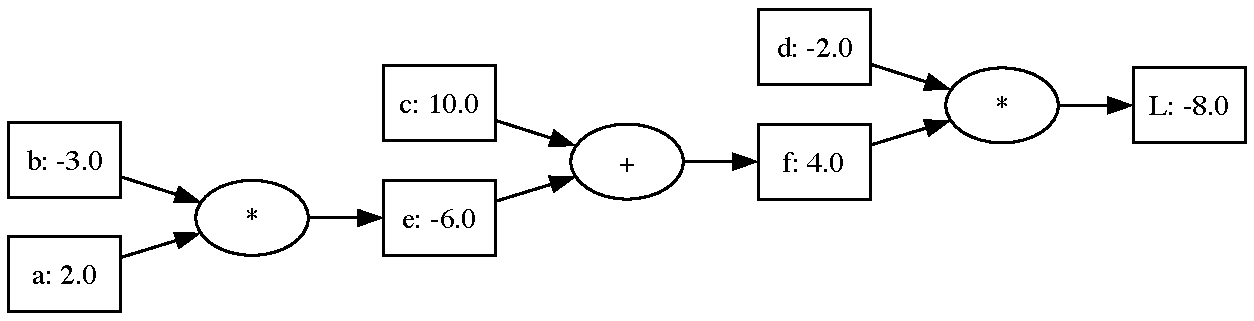
\includegraphics[width=0.9\textwidth]{figs/010-racunski-graf.pdf}}
  \caption[6pt]{}
  \label{fig:racunski-graf}
\end{figure*}

Lotimo se odvajanj. Opazimo, da je naša funkcija $L$ neposredno odvisna od spremenljivk $d$ in $f$, zato je najlažje začeti z odvajanjem po teh spremenljivkah. Najprej za spremenljivko $d$. Zanima nas torej, kako se spremeni vrednost funkcije $L$, če spremenimo vrednost $d$-ja:

\[
\frac{\partial L}{\partial d} = \lim_{h \to 0} \frac{f(d+h) - fd}{h} = \lim_{h \to 0} \frac{fd + fh - fd}{h} = \lim_{h \to 0} \frac{fh}{h} = f
\]
%
\noindent Ker je vrednost \( f = 4 \), je torej gradient funkcije $L$ po spremenljivi (ali parametru) $d$ torej enak:

\[
\frac{\partial L}{\partial d} = f = 4
\]

Na podoben način izračunajma še odvod funkcije \( L \) po spremenljivki \( f \):
\[
\frac{\partial L}{\partial f} = \lim_{h \to 0} \frac{(f+h)d - fd}{h} = \lim_{h \to 0} \frac{fd + hd - fd}{h} = \lim_{h \to 0} \frac{hd}{h} = d
\]
%
\noindent Ker vemo, da je \( d = -2 \), je torej odvod po spremenljivki \( f \) enak:
%
\[
\frac{\partial L}{\partial f} = d = -2
\]

Za izračun odvoda po parametru \( c \) rabimo poseči po verižnem pravilu:

\[
\frac{\partial L}{\partial c} = \frac{\partial L}{\partial f} \frac{\partial f}{\partial c}
\]
%
\noindent kjer je \( \frac{\partial f}{\partial c} \) enak:
%
\[
\frac{\partial f}{\partial c} = \frac{\partial (e+c)}{\partial c} = \lim_{h \to 0} \frac{(e+c+h) - (e+c)}{h} = \lim_{h \to 0} \frac{e+c+h-e-c}{h} = \lim_{h \to 0} \frac{h}{h} = 1
\]
%
\noindent Ker smo že izračunali \( \frac{\partial L}{\partial f} = d = -2 \), je torej:

\[
\frac{\partial L}{\partial c} = d \times 1 = -2
\]

Podobno izračunamo parcialni odvod po spremenljivki e, ki bo prav tako enak -2. Ostane name še izračun parcialnih odvodov po spremenljivkah a in b. Začnimo s spremenljivko a:

\[
\frac{\partial L}{\partial a} = \frac{\partial L}{\partial e} \frac{\partial e}{\partial a}
\]

Odvod \( \frac{\partial L}{\partial e} \) poznamo, enak je -2, \( \frac{\partial e}{\partial a} \) pa izračunajmo:

\[
\frac{\partial e}{\partial a} = \frac{\partial (ab)}{\partial a} = \lim_{h \to 0} \frac{(a+h)b - ab}{h} = \lim_{h \to 0} \frac{ab + hb - ab}{h} = \lim_{h \to 0} \frac{hb}{h} = b
\]

Ker je \( b = -3 \) in \( \frac{\partial L}{\partial e} = -2 \), je \( \frac{\partial L}{\partial a} \) torej enak 6. Podobno bi lahko izračunali še, da je \( \frac{\partial L}{\partial b} = -4 \). 

Zgornje računanje ``na roke'' je malce zamudno in pisci tega besedila vedo, da imajo opravka z bralci, ki vse to dobro razumejo in znajo. A smu to samo želeli izpostaviti, da nam pri računanju parcialnih odvodov lahko močno koristi, če funkcijo, ne glede na to, kako kompleksna je, ponazorimo z računskim grafom, ki tipično uporablja neke osnovne in enostavno odvedljive operacije, ter odvode potem računamo vzvratno z verižnim pravilom. 

Spoznali smo tudi, da ko imamo v računskih grafih opravka z vsotami,  ``skopiramo'' vrednost odvoda od staršev vozlišča, pri množenju pa ta odvod pomnožimo še z vrednostjo sosednjega (sestrskega) vozlišča. Paziti sicer moramo pri funkcijah, kjer je staršev določenega vozlišča več: tam bomo morali vplive na starše vozlišča prištevati. Vse to, torej postopek odvajanja z uporabo računskega grafa, pa nam bo zelo prav prišel v naslednjem poglavju, ko bomo sestavljali kodo za strojno odvajanje.
\chapter{Strojno odvajanje}

V prejšnjem poglavju smo videli, da nam pri odvajanju funkcij koristi, 
če jih zapišemo v obliki računskega grafa in se nato pri odvajanju 
po grafu sprehodimo od konca proti začetku. Ta vzvratni »sprehod« 
(angl.\ \emph{back-propagation}) ustreza verižnemu pravilu odvajanja, 
pri čemer si vse vmesne rezultate zapomnimo in jih izračunamo natanko enkrat.

\marginnote{Pri razvoju postopka in kode za strojno odvajanje smo se močno zgledovali po izjemnem predavanju Andreja Karpathyja \emph{The spelled-out intro to neural networks and backpropagation: building micrograd}.}
Na osnovi tega vzvratnega sprehoda bomo zgradili algoritem oziroma 
implementirali kodo za strojno odvajanje. Pričeli bomo pri njegovem 
okostju~-- računskem grafu. Najprej bomo implementirali vozlišče grafa, 
mu dodali podatke o njegovih predhodnikih ter preverili, ali lahko 
računski graf uporabimo za izračun funkcijskih vrednosti 
(angl.\ \emph{forward computation}). Ko bomo s tem zadovoljni, 
bomo implementirali še izračun gradientov. Postopek bomo razvijali 
postopoma in ga zaključili z demonstracijo uporabnosti.

\section{Vozlišča v računskem grafu}

Čas je, da za strojno odvajanje spišemo tudi kodo, in sicer v programskem
jeziku Python. Začnimo s predstavitvijo vozlišča v računskem grafu, ki ga
implementiramo z razredom \texttt{Value}, saj bo ta hranil vrednost neke
spremenljivke:

\vspace*{3mm}
\begin{lstlisting}
class Value:
    def __init__(self, data):
        self.data = data

    def __repr__(self):
        return f"Value({self.data})"
\end{lstlisting}

Vozlišče tako hrani podatek \texttt{data} in zna svojo vrednost tudi
smiselno izpisati. Uporaba razreda je preprosta:

\vspace*{3mm}
\begin{lstlisting}
>>> a = Value(2.0)
>>> a
Value(2.0)
\end{lstlisting}

\section{Računski graf}

Nad vozlišči oziroma spremenljivkami, ki jih vozlišča predstavljajo, bi radi
izvajali računske operacije. Na primer, želeli bi, da razred \texttt{Value}
podpira naslednjo uporabo:

\vspace*{3mm}
\begin{lstlisting}
>>> a = Value(2.0)
>>> b = Value(-3.0)
>>> e = a + b
>>> g = e * b
\end{lstlisting}

Razred za vozlišče v računskem grafu zato razširimo z implementacijo vsote in
produkta. Ker gradimo graf, bomo povezave v njem hranili tako, da si bo vozlišče
zapomnilo svoje predhodnike. Za namene izrisa grafa bomo shranili tudi oznako
matematične operacije in ime spremenljivke, ki jo hrani vozlišče. Opozorimo, da
teh oznak in imen v resnih aplikacijah strojnega učenja (na primer v nevronskih
mrežah) praviloma ne potrebujemo; pri spoznavanju strojnega odvajanja pa ta
funkcionalnost ne škodi.

\vspace*{3mm}
\begin{lstlisting}
class Value:
    def __init__(self, data, _children=(), _op='', label=''):
        self.data = data
        self.label = label
        self._prev = set(_children)
        self._op = _op

    def __repr__(self):
        return f"Value({self.label}: {self.data})"
    
    def __add__(self, other):
        out = Value(self.data + other.data, (self, other), '+')
        return out
    
    def __mul__(self, other):
        out = Value(self.data * other.data, (self, other), '*')
        return out
\end{lstlisting}

Zgradimo računski graf za enostavno funkcijo, ki smo jo spoznavali v prejšnjem
poglavju:

\vspace*{3mm}
\begin{lstlisting}
a = Value(2.0, label='a')
b = Value(-3.0, label='b')
c = Value(10.0, label='c')
d = Value(-2.0, label='d')

e = a * b
e.label = 'e'
f = e + c
f.label = 'f'
L = f * d
L.label = 'L'
\end{lstlisting}

\noindent Preverimo delovanje:

\vspace*{3mm}
\begin{lstlisting}
>>> L
Value(L: -8.0)
>>> L._prev
{Value(d: -2.0), Value(f: 4.0)}
\end{lstlisting}

Dela!

\section{Izris računskega grafa}

\marginnote{Graphviz sta razvila Stephen North in Ellie Gansner v AT\&T Labs -- Research v začetku devetdesetih let (1991). Projekt je nastal kot del raziskav na področju vizualizacije grafov in avtomatskega risanja diagramov ter je bil kasneje objavljen kot odprtokodni projekt.}
%
Računski graf bi bilo smiselno tudi izrisati. Za to bomo uporabili knjižnico \texttt{graphviz}, odprtokodno orodje za risanje grafov, ki je posebej primerno za izris usmerjenih in neusmerjenih grafov, kjer vozlišča in povezave predstavljajo podatke ali odnose. Graphviz za opis grafa uporablja jezik DOT, preprost tekstovni zapis za opis vozlišč in povezav. V Pythonu ta opis nadomestimo s funkcijskimi klici.

Za začetek si oglejmo enostaven primer uporabe:

\begin{marginfigure}
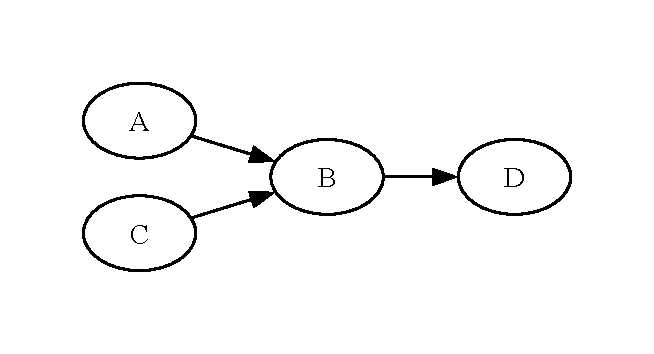
\includegraphics[width=\linewidth]{figs/020-enostavni-graf.pdf}
\end{marginfigure}
%
\vspace*{3mm}
\begin{lstlisting}
import graphviz
from IPython.display import display
dot = graphviz.Digraph()
dot.node('A')
dot.node('B')
dot.edge('A', 'B')
dot.node('C')
dot.edge('C', 'B')
dot.node('D')
dot.edge('B', 'D')
display(dot)
\end{lstlisting}

Koda za izris našega računskega grafa je nekoliko kompleksnejša
(tudi tu sledimo pristopu Andreja Karpathyja). Posebej pomembna je
funkcija \texttt{trace}, ki se rekurzivno sprehodi po grafu, zbere
vozlišča in povezave ter jih topološko uredi. Ta ureditev nam bo
kasneje koristila tudi pri računanju gradientov.

\vspace*{3mm}
\begin{lstlisting}
def trace(root):
    nodes, edges = set(), set()
    def build(v):
        if v not in nodes:
            nodes.add(v)
            for child in v._prev:
                edges.add((child, v))
                build(child)
    build(root)
    return nodes, edges

def draw_dot(root, format='svg', rankdir='LR'):
    """
    format: png | svg | ...
    rankdir: TB (top to bottom graph) | LR (left to right)
    """
    assert rankdir in ['LR', 'TB']
    nodes, edges = trace(root)
    dot = Digraph(format=format, graph_attr={'rankdir': rankdir})
    
    for n in nodes:
        dot.node(name=str(id(n)), label = "{ %s: %.1f }" % \
         (n.label, n.data), shape='record')
        if n._op:
            dot.node(name=str(id(n)) + n._op, label=n._op)
            dot.edge(str(id(n)) + n._op, str(id(n)))
    
    for n1, n2 in edges:
        dot.edge(str(id(n1)), str(id(n2)) + n2._op)
    
    return dot
\end{lstlisting}

Sedaj lahko izrišemo naš računski graf:

\vspace*{3mm}
\begin{lstlisting}
>>> draw_dot(L)
\end{lstlisting}

\begin{figure*}
\includegraphics[width=\linewidth]{figs/020-računski-graf.pdf}
\end{figure*}

Vse je pravilno izračunano. Manjkajo le še odvodi.

\section{Računanje gradientov}

Do tu nam je šlo lepo, a vse, kar smo do sedaj naredili, je bilo računanje vrednosti funkcij. Takih enostavnih, z vsotami in produkti. Manjka nam (vsaj) še izračun gradientov. Te računamo po verižnem pravilu, od zadaj naprej. Torej, od končnih vozlišč s končno vrednostjo funkcije do začetnih vozlišč oziroma vhodnih parametrov. 

Gradiente bomo torej strojno računali tako, da bodo te vozliščem računali njihovi nasledniki, in sicer tako, da jim bodo ustrezno prišteli vrednost lastnega gradienta (vsota) oziroma k tej pomnožili še vrednost sosednega vozlišča (produkt). Vse to bo implementirano v funkciji \texttt{\_backward()}, ki bo lastna vsaki od implementiranih operacij (zaenkrat sta tu le vsota in produkt, kasneje bomo dodali še kakšno drugo funkcijo). Za končni izračun gradienta se moramo sprehoditi po računskemu grafu. To bo storila funkcija \texttt{backward()}, ki se bo najprej topološko uredila vozlišča, potem pa se po njih sprehodila in v vsakem klicala \texttt{\_backward()}.

Še nekaj razmislekov preden razkrijemo zadnjo razširitev naše kode. Gradiente nasledniki prištevajo, ne nastavijo. Na začetku morajo biti gradienti zato postavljeni na vrednosti 0. Prištevanje pa nam koristi v primeru, da ima vozlišče več kot enega naslednika. Npr., v funkciji \( b = a + a \) vsak \( a \) "prinese" po eno 1-ko k odvodu. V nevronskih mrežah, na primer, bodo imela vozlišča računskega grafa tipično veliko naslednikov, in vsak od njih bo k gradientu vozlišča prispeval svojo vrednost. 

Upoštevamo tudi, da je odvod zadnjega vozlišča, torej odvod končne spremenljivke \( L \) po \( L \)-u enak 1. Začnemo torej s to vrednostjo odvoda in jo razširimo od tega, zadnjega vozlišča, nazaj proti začetnim vozliščem. Tu je koda, kjer za vsako od operacij implementiramo funkcijo \texttt{\_backward()}:

\vspace*{3mm}
\begin{lstlisting}
class Value:
    def __init__(self, data, _children=(), _op='', label=''):
        self.data = data
        self.label = label
        self.grad = 0.0
        self._backward = lambda: None
        self._prev = set(_children)
        self._op = _op

    def __repr__(self):
        return f"Value({self.label}: {self.data})"
    
    def __add__(self, other):
        out = Value(self.data + other.data, (self, other), '+')

        def _backward():
            self.grad += 1.0 * out.grad
            other.grad += 1.0 * out.grad
        out._backward = _backward
        return out
    
    def __mul__(self, other):
        out = Value(self.data * other.data, (self, other), '*')

        def _backward():
            self.grad += other.data * out.grad
            other.grad += self.data * out.grad
        out._backward = _backward
        return out
\end{lstlisting}

Manjka le še uporaba funkcij \texttt{\_backward()}. Spomnimo se (morda preveč ponavljamo, a je pomembno), da za dano vozlišče funkcija \texttt{\_backward()} zabeleži vpliv neposrednih predhodnikov danega vozlišča na gradient vozlišča. Če želimo izračunati gradiente za vse spremenljivke v računskem grafu, moram pričeti od zadaj, in v topološkem redu od zadaj naprej za vsako vozlišče pognati \texttt{\_backward()}. Implementacijo takega vzvratnega razširjanja gradientov dodamo v razred \texttt{Value}:

\vspace*{3mm}
\begin{lstlisting}
    def backward(self):
        # topological ordering of the nodes
        topo = []
        visited = set()
        def build_topo(v):
            v.grad = 0
            if v not in visited:
                visited.add(v)
                for child in v._prev:
                    build_topo(child)
                topo.append(v)
        build_topo(self)

        # application of chain rule
        self.grad = 1
        for v in reversed(topo):
            v._backward()
\end{lstlisting}

Preskusimo njeno delovanje na naši enostavni funkciji, torej na tej, za katero smo gradiente računali ročno v prejšnjem poglavju:

\vspace*{3mm}
\begin{lstlisting}
a = Value(2.0, label='a')
b = Value(-3.0, label='b')
c = Value(10.0, label='c')
d = Value(-2.0, label='d')

e = a * b
e.label = 'e'
f = e + c
f.label = 'f'
L = f * d
L.label = 'L'

L.backward()
\end{lstlisting}

Izpišimo še vrednosti gradientov:

\vspace*{3mm}
\begin{lstlisting}
>>> a.grad, b.grad, c.grad, d.grad
(6.0, -4.0, -2.0, 4.0)
\end{lstlisting}

Juhu! Dela. Oziroma, bolje rečeno, pravilno izračuna vrednosti gradientov za našo enostavno funkcijo. Enostavno zato, ker ta samo sešteva in množi. Spodaj je še izris računskega grafa z odvodi:

\begin{figure*}
\includegraphics[width=\linewidth]{figs/020-računski-graf-odvodi.pdf}
\end{figure*}

\section{Konstante, negacija, potenciranje}

Pri malce bolj kompleksnih funkcijah bi želeli v naših računskih grafih obravnavati tudi konstate, računali razlike, potence... Oziroma, delali z izrazi, kot so na primer spodnji:

\vspace*{3mm}
\begin{lstlisting}
>>> a = Value(3, 'a')
>>> b = Value(42, 'b')
>>> a + 10
>>> -13 + a
>>> a - b
>>> (a + b) ** 3
\end{lstlisting}

Pri vseh teh nam naša trenutna implementacija vrne napako. Potrebno jo bo zato razširiti. Za operacije s konstantami bomo avtomatsko dodali novo vozlišče, za to, da bodo te lahko v naših operacijah tudi na levi strani, bomo implementirali funkcije, kot je \texttt{\_\_radd\_\_}, odštevanje bomo implementirali s seštevanje z negativno vrednostjo desnega operanda, spisali pa bomo tudi novo operacijo za potenciranje. Spodaj je tako razširjena implementacija razreda \texttt{Value}:

\vspace*{3mm}
\begin{lstlisting}
class Value:
    def __init__(self, data, _children=(), _op='', label=''):
        self.data = data
        self.label = label
        self.grad = 0.0
        self._backward = lambda: None
        self._prev = set(_children)
        self._op = _op

    def __repr__(self):
        return f"Value({self.label}: {self.data})"
    
    def __add__(self, other):
        other = other if isinstance(other, Value) else Value(other)
        out = Value(self.data + other.data, (self, other), '+')

        def _backward():
            self.grad += out.grad
            other.grad += out.grad
        out._backward = _backward

        return out
    
    def __mul__(self, other):
        other = other if isinstance(other, Value) else Value(other)
        out = Value(self.data * other.data, (self, other), '*')

        def _backward():
            self.grad += other.data * out.grad
            other.grad += self.data * out.grad
        out._backward = _backward
        return out
    
    def __pow__(self, other):
        out = Value(self.data ** other, (self, ), f'**{other}')

        def _backward():
            self.grad += other * (self.data ** (other - 1)) * out.grad
        out._backward = _backward
        return out
    
    def __radd__(self, other):  # other + self
        return self + other
    
    def __neg__(self): # - self
        return self * -1
    
    def __sub__(self, other):
        return self + (-other)
    
    def __rsub__(self, other):  # other - self
        return other + (-self)

    def __rmul__(self, other):  # other * self
        return self * other
\end{lstlisting}

Iz zgornjega zapisa smo izpustili funkcijo \texttt{backward()}, ki ostane enaka kot prej. S kodo, kot jo imamo spisano zgoraj, lahko sedaj implementirano gradientni sestop za funkcijo iz prejšnjega poglavja:

\vspace*{3mm}
\begin{lstlisting}
a = Value(0, label='a')
for _ in range(50):
    L = a**2 - 10 * a + 28
    backward(L)
    a.data -= 0.1 * a.grad
    print(L.data, a.data)
\end{lstlisting}

Tu je čas za bralca, da preskusi delovanje naše kode, jo morda preoblikuje v knjižnico in doda izračun in odvajanje za še kakšne dodatne funkcije. Mi pa se bomo spustili v nove podvige v naslednjem poglavju, ko bomo to kodo za avtomatsko odvajanje uporabili na bolj resnih primerih, kjer bodo (kriterijske) funkcije uporabljale tudi zunanje podatke in na primer tako implementirale iskanje modela za linearno regresijo ali njeno regularizirano inačico. Z zgornjimi, in morda še kakšnimi drugi manjšimi razširitvami, smo sedaj torej pripravljeni za ``resno'' uporabo naše male knjižnice za avtomatsko odvajanje.
\chapter{Linearna regresija}

To poglavje pravzaprav ni čisto o linearni regresiji.\marginnote{Linearna regresija izvira iz metode najmanjših kvadratov, ki jo je leta 1805 prvi objavil Adrien-Marie Legendre, leta 1809 pa jo je Carl Friedrich Gauss pri analizi astronomskih opazovanj dodatno povezal z normalno porazdelitvijo. Izraz {\em regresija} je pozneje, v 1880-ih, uvedel Francis Galton pri preučevanju dednosti. Opazil je, da imajo zelo visoki starši sicer pogosto visoke otroke, vendar so ti v povprečju nekoliko bližje populacijskemu povprečju; ta pojav je poimenoval {\em regresija proti sredini} (angl. {\em regression toward the mean}).} Je bolj o tem, kako uporabimo strojno odvajanje za gradnjo modelov iz podatkov. A bomo sproti razmišljali tudi o linearni regresiji, verjetju in kriterijskih funkcijah. Začnemo z univariatno linearno regresijo, jo razširimo na multivariatno, vse skupaj poskusimo še na bolj resnih podatkih in razmislimo, ali na odkriti modeli lahko kako pomagajo pri razlagi podatkov.

\section{Podatki in kaj sploh želimo}

Pri \emph{univariatni regresiji} obravnavamo podatke, ki vsebujejo eno neodvisno spremenljivko $x$ in eno odvisno spremenljivko $y$. Cilj je opisati oziroma aproksimirati funkcijsko povezavo med njima z modelom linearne oblike

\[
\hat{y}(x) = wx + b ,
\]
%
kjer je $w$ smerni koeficient (utež), ki določa naklon premice, $b$ pa prosti člen oziroma presečišče z ordinatno osjo. Model je torej v celoti določen z dvema parametroma, $w$ in $b$.

Pri učenju modela imamo na voljo učno množico podatkov, sestavljeno iz parov vrednosti $(x_i, y_i)$, na primer:

\[
\begin{array}{S S}
\hline
{x_i} & {y_i} \\
\hline
1.4 & -2.0 \\
-4.7 & -18.1 \\
-2.2 & -1.9 \\
-2.8 & -4.4 \\
2.4 & 6.5 \\
\hline
\end{array}
\]

Za vsak učni primer model napove vrednost $\hat{y}_i = wx_i + b$, ki se lahko razlikuje od dejanske vrednosti $y_i$. Napako napovedi za posamezen primer zapišemo kot

\[
\varepsilon_i = \hat{y}_i - y_i .
\]

Ker nas predznak napake ne zanima \marginnote{Idejo o vsoti kvadriranih napak smo tu uvedli rokohitrsko. K temu, zakaj tako, nekoliko kasneje.}, napake kvadriramo in izračunamo njihovo povprečje. Tako dobimo cenovno funkcijo oziroma funkcijo izgube, ki je pri dani učni množici odvisna samo od parametrov modela:

\[
J(w,b) = \frac{1}{n} \sum_{i=1}^{n} (\hat{y}_i - y_i)^2
      = \frac{1}{n} \sum_{i=1}^{n} (wx_i + b - y_i)^2 .
\]

Cenovna funkcija meri, kako dobro izbrani parametri $w$ in $b$ opisujejo podane podatke. Cilj učenja je poiskati takšni vrednosti parametrov, pri katerih je vrednost cenovne funkcije minimalna:

\[
(w^\ast, b^\ast) = 
\arg\min_{w,b} J(w,b).
\]

Par $(w^\ast, b^\ast)$ predstavlja optimalna parametra modela glede na dano učno množico in ga dobimo z učenja modela, oziroma strojnem učenju iz podatkov. Strojno učenje je tu torej postopek, kjer za dano učno množico in izbrano strukturo modela poiščemo take parametre modela, da ti optimizirajo izbrano kriterijsko funkcijo.

\section{Univariatna linearna regresija v Pythonu}

Linearno regresijo implementirajmo v pythonovskem razredu \texttt{LinReg}. Pri njeni implementaciji uporabimo razred \texttt{Value}, kot smo ga razvili v prejšnjem poglavju in za kodo od tu naprej shranili v knjižnici \texttt{agrad}:

\vspace*{3mm}
\begin{lstlisting}
from agrad import Value

class LinReg:
    def __init__(self):
        self.w = Value(random.uniform(-1,1), label='w')
        self.b = Value(0.0, label='b')
    
    def __call__(self, x):
        return self.w * x + self.b
    
    def parameters(self):
        return [self.w, self.b]

    def loss(self, xs, ys):
        yhats = [self(x) for x in xs]
        return sum([(y - yhat)**2  for y, yhat in zip(ys, yhats)])
    
    def __repr__(self):
        return f"LinReg(w={self.w.data:.3f}, b={self.b.data:.3f})"
\end{lstlisting}

V funkciji \texttt{\_\_init\_\_()} določimo začetne vrednosti parametrov modela. Klic modela implementiramo v funkciji \texttt{\_\_call\_\_()}. Razred \texttt{LinReg} vrne tudi seznam parametrov modela, ki ga bomo rabili pri posodabljanju parametrov v gradientnem sestopu. Izjemno pomembna pa je funkcija \texttt{loss()}, ki pri danih vrednostih parametrov in dani učni množici izračuna izgubo.

Za prvi test delovanja \texttt{LinReg} poskusimo uporabiti naš razred za izračun linearne regresije pri določenih parametrih modela:

\vspace*{3mm}
\begin{lstlisting}
>>> model = LinReg()
>>> model.w = Value(10); model.b = Value(3)
>>> model(10)
Value(: 103)
\end{lstlisting}

Na manjši učni množici, na primer:

\vspace*{3mm}
\begin{lstlisting}
import random
random.seed(42)
n = 5
xs = [random.uniform(-5, 5) for _ in range(n)]
ys = [2*x -1 + random.gauss(0, 4) for x in xs]
\end{lstlisting}
%
lahko sedaj preverimo

\vspace*{3mm}
\begin{lstlisting}
>>> lr = LinReg()
>>> lr
LinReg(w=0.011, b=0.000)
>>> lv = lr.loss(xs, ys)
>>> lv
Value(: 78.49574710788079)
\end{lstlisting}

Izguba (vsota kvadratov napak) je seveda velika, saj je zgornji model še nenaučen, naključen. Zanimiv pa je računski graf za izgubo. Koda za njegov izris je:

\vspace*{3mm}
\begin{lstlisting}
from agrad import draw_dot
lv.backward()
dot = draw_dot(lv)
dot.render('a', format='pdf', cleanup=True)
\end{lstlisting}
%
Pazljivi bralec bo seveda opazil, da smo pred izrisom računskega grafa izračunali gradiente. Implementacijo izrisa smo skrili v knjižnico agrad, a je točno taka kot v prejšnjem poglavju in je tu ne rabimo ponovno izpostavljati. Računski graf za našo funkcijo izgube je tu, kljub manjhni učni množici, že kar kompleksen, tudi zato, ker vključuje vsoto preko vseh petih učnih primerov:

\begin{figure*}
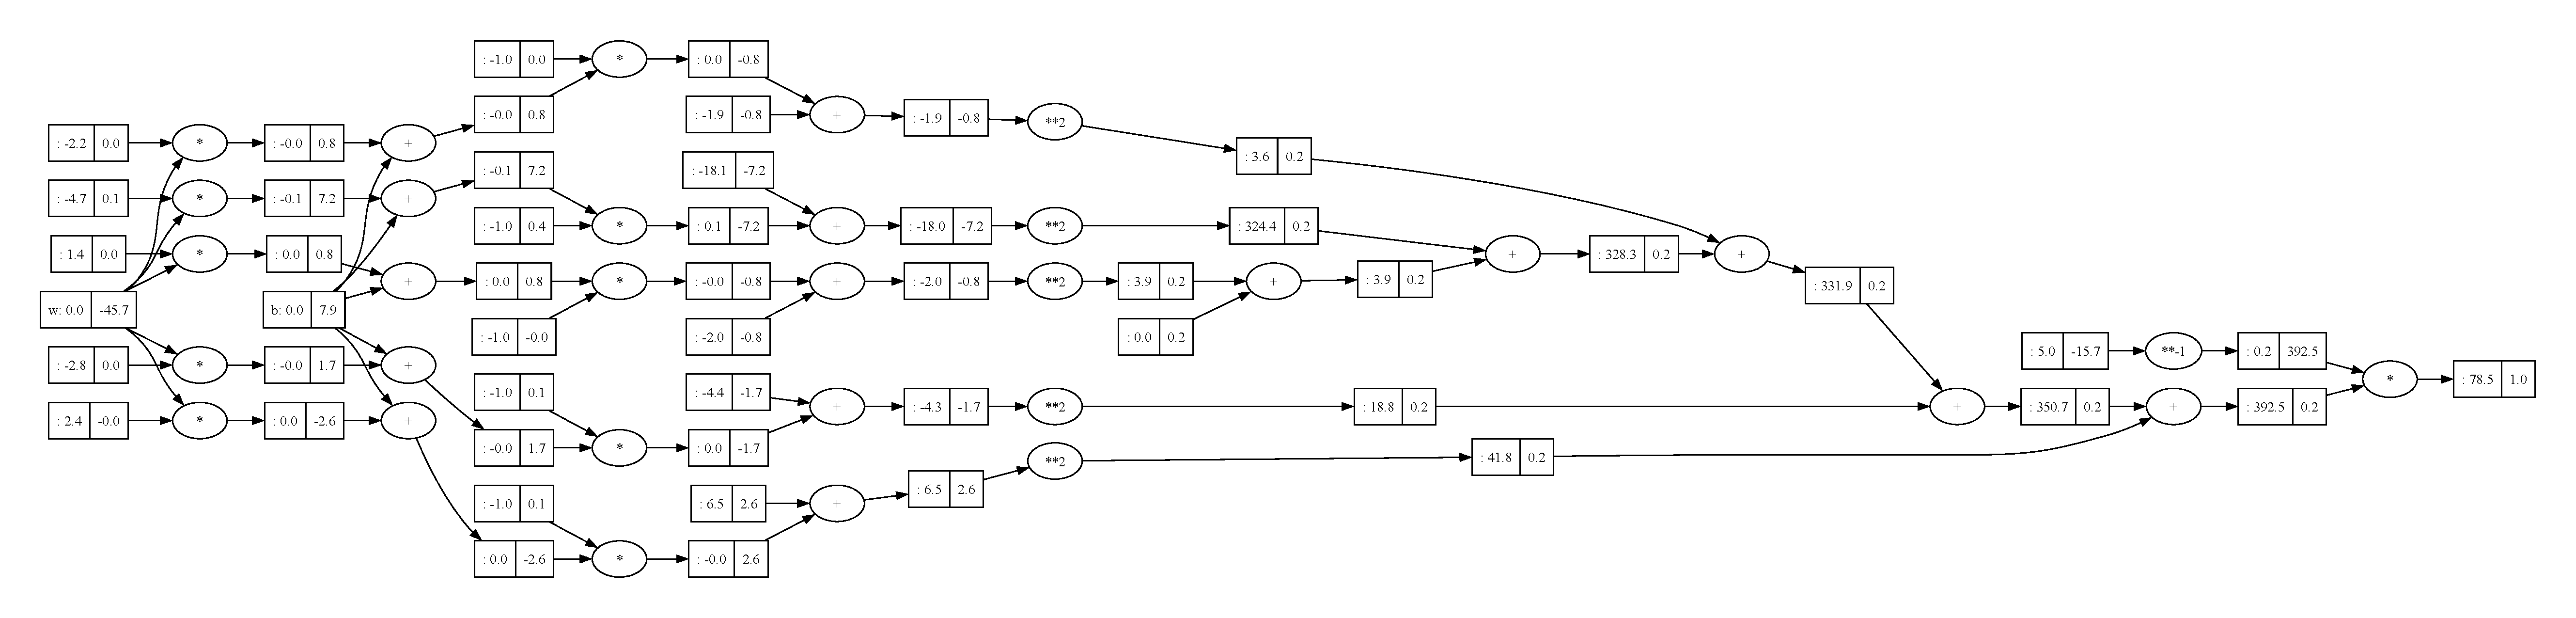
\includegraphics[width=\linewidth]{figs/030-linreg-graph.pdf}
\end{figure*}

\section{Učenje}

Ah, končno! Vse je nared, da iz primerov izračunamo {\em prave} vrednosti parametrov našega univariatnega modela. Spomnimo: z računskim grafom bomo računali parcialne odvode funkcije za parametre modela, te vsakič malo popravili in postopek ponavljali do konvergence oziroma za neko vnaprej dano število ponovitev.

Sestavimo sedaj funkcijo za učenje, ki implementira gradientni sestop. Spodnja optimizacijska funkcija je pravzaprav splošna, uporabili bi jo lahko za kakršenkoli model, ki pri učenju uporablja primere z razredom.

\vspace*{3mm}
\begin{lstlisting}
def train(model, xs, ys, learning_rate=0.001, n_epochs=1000):
    for k in range(n_epochs):
        # compute loss
        loss = model.loss(xs, ys)

        # compute gradients
        for p in model.parameters():
            p.grad = 0
        loss.backward()

        # update
        for p in model.parameters():
            p.data -= learning_rate * p.grad

        if k % 50 == 0:
            print(f"{k:3} Loss: {loss.data:5.3f} {model}")
    return model
\end{lstlisting}
%
V vsaki iteraciji smo zgradili računski graf za našo izgubo, gradiente parametrov modela nastavili na nič (k tem vrednostim izračunane gradiente prištevamo), nato gradiente izračunali, in popravili vrednost parametrov modela.

Čas je za učenje:

\vspace*{3mm}
\begin{lstlisting}
>>> model = train(LinReg(), xs, ys, learning_rate=0.01, n_epochs=500)
  0 Loss: 130.147 LinReg(w=-0.326, b=-0.102)
 50 Loss: 16.793 LinReg(w=2.578, b=-0.745)
100 Loss: 16.778 LinReg(w=2.566, b=-0.827)
150 Loss: 16.775 LinReg(w=2.560, b=-0.864)
200 Loss: 16.774 LinReg(w=2.558, b=-0.880)
250 Loss: 16.774 LinReg(w=2.557, b=-0.887)
300 Loss: 16.774 LinReg(w=2.556, b=-0.890)
350 Loss: 16.774 LinReg(w=2.556, b=-0.891)
400 Loss: 16.774 LinReg(w=2.556, b=-0.892)
450 Loss: 16.774 LinReg(w=2.556, b=-0.892)
\end{lstlisting}
%
Gradientni sestop je v nekaj sto iteracijah torej našel (skoraj) pravi model, torej ta s parametri \( w=2 \) in \( b=-1 \). Bralcu tu prepuščamo eksperimente s spremenjeno stopnjo učenja. Povejmo le, da za te podatke in ta model učenje lahko konvergira hitreje, lahko pa z večanjem stopnje učenja pridemo do napake tipa \texttt{`OverflowError: (34, 'Result too large')}. Zakaj?

\section{Paketno učenje}

Bralec teh zapiskov bi lahko pripomnil, da je primer v prejšnjem poglavju s samo petimi primeri bil preenostaven in da bi znali tako linearno regresijo narediti tudi "na roko". Morda, čeprav bi bilo računov že za tak majhen primer izjemno veliko. Zato pa je zdaj pravi trenutek, da preskusimo našo implementacijo na večji množici podatkov:

\vspace*{3mm}
\begin{lstlisting}
random.seed(42)
n = 1000
xs = [random.uniform(-10, 10) for _ in range(n)]
ys = [2*x + 1 + random.gauss(0, 5) for x in xs]
\end{lstlisting}

\begin{marginfigure}
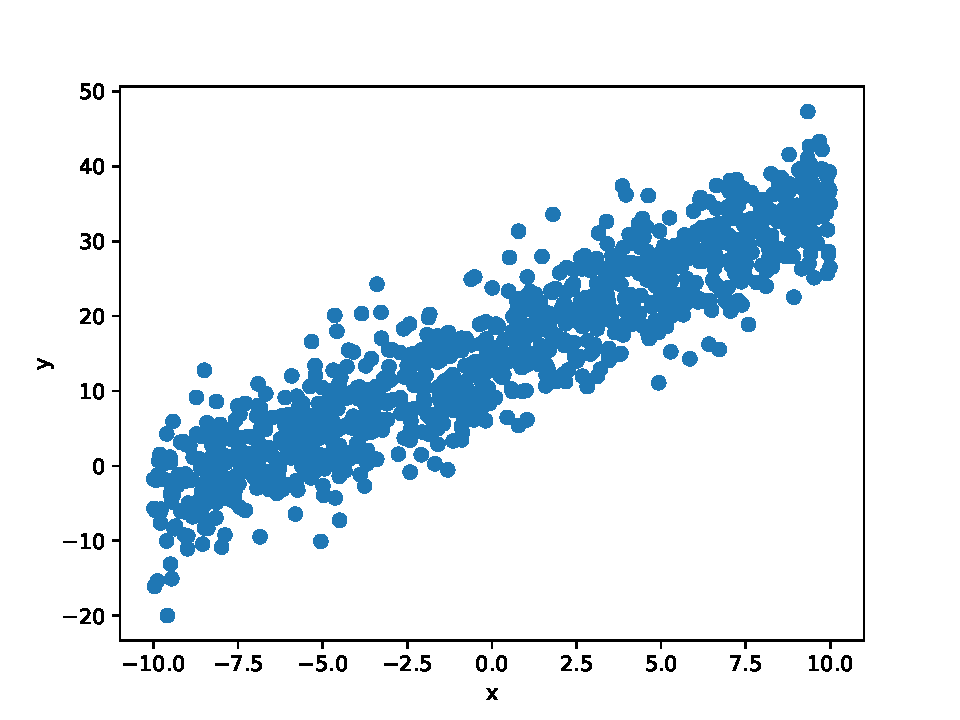
\includegraphics[width=\linewidth]{figs/030-unidata.pdf}
\end{marginfigure}

Pri velikem številu primerov računski graf za funkcijo izgube močno naraste in učenje lahko zato postane precej počasno. Primerov je morda dovolj za drugačen pristop, pri katerem lahko izgubo računamo samo iz vzorca učne množice. Takemu učenju pravimo paketno (angl. {\em batch learning}), preprosto pa ga implemenira spodnja funkcija, ki jo dodajmo razredu \texttt{LinReg}:

\vspace*{3mm}
\begin{lstlisting}
    def batch_loss(self, xs, ys, m=10):
        indices = random.sample(range(len(xs)), m)
        batch_xs = [xs[idx] for idx in indices]
        batch_ys = [ys[idx] for idx in indices]
        return self.loss(batch_xs, batch_ys)
\end{lstlisting}

Za paketno učenje moramo sedaj spremeniti le vrstico, ki vpelje funkcijo izgube. Ta je sedaj 

\vspace*{3mm}
\begin{lstlisting}
loss = model.batch_loss(xs, ys, batch_size)
\end{lstlisting}
%
predvideva pa, da meta-parametrom učne metode dodamo še \texttt{batch\_size} s privzeto vrednostjo, na primer 10.

Pri paketnem učenju izguba na celotni učni množici ne bo padala monotono:
\vspace*{3mm}
\begin{lstlisting}
>>> model = train(LinReg(), xs, ys, learning_rate=0.01, n_epochs=500)
  0 Loss: 442.514 LinReg(w=0.620, b=0.266)
 50 Loss: 111.536 LinReg(w=1.792, b=9.632)
100 Loss: 12.292 LinReg(w=1.868, b=12.622)
150 Loss: 24.878 LinReg(w=2.042, b=13.802)
200 Loss: 46.238 LinReg(w=1.705, b=14.689)
250 Loss: 30.237 LinReg(w=1.685, b=14.732)
300 Loss: 23.126 LinReg(w=2.113, b=14.865)
350 Loss: 29.744 LinReg(w=1.662, b=14.941)
400 Loss: 25.119 LinReg(w=2.435, b=14.894)
450 Loss: 10.819 LinReg(w=1.884, b=14.988)
\end{lstlisting}
%
Tudi naš model ni ravno najbolj idealen\marginnote{Kar naenkrat smo pridelali vrsto meta parametrov pri našem učenju. To so parametri, ki vplivajo na postopek učenja, vključujejo pa stopnjo učenja, število epoh, velikost paketa. Bralcu tu prepustimo razmislek, kako te parametre nastavimo, se bomo pa z njimi ukvarjali še v naslednjih poglavjih.}, so se pa parametri modela precej približali tem, s katerimi smo podatke generirali. Paketno učenje je sicer veliko hitrejše kot gradientni spust, kjer vsakič računamo izgubo na celotni učni množici, moramo pa biti pazljivi pri nastavitvah stopnje učenja in velikosti paketov podatkov.

\section{Multivariatna linearna regresija}

Razširimo naš model linearne regresije na multivariatno, to je, na modele, ki na vhodu sprejmemo več vhodnih, neodvisnih spremenljivk, ki jim v strojnem učenju pravimo tudi atributi. 

\vspace*{3mm}
\begin{lstlisting}
random.seed(42)
n = 1000
X = [[random.uniform(-10, 10) for _ in range(3)] for _ in range(n)]
ys = [2*x[0] + 3*x[1] - x[2] + 1 + random.gauss(0, 5) for x in X]
\end{lstlisting}

Prav velikih sprememb v kodi za učenje ne bi smelo biti\marginnote{Našo implementacijo bi se dalo izboljšati tudi tako, da bi shranili imena spremenljivk. Ta postanejo pomembna pri vsakem poskusu razumevanja modela.}. V razredu \texttt{LinReg} funkciji \texttt{loss()} in \texttt{batch\_loss()} ostaneta taki, kot sta bili, ostale pa malce spremenimo, 

\vspace*{3mm}
\begin{lstlisting}
class LinReg:
    def __init__(self, n_inputs):
        self.weights = [Value(random.uniform(-1,1), label=f'w{i}') 
                        for i in range(n_inputs)]
        self.b = Value(0.0, label='b')

    def __call__(self, x):
        # x is a list of input values
        return sum(w * xi for w, xi in zip(self.weights, x)) + self.b

    def parameters(self):
        return self.weights + [self.b]

    def __repr__(self):
        weights_str = ', '.join(f'w{i}={w.data:.3f}' 
                                for i, w in enumerate(self.weights))
        return f"LinReg({weights_str}, b={self.b.data:.3f})"
\end{lstlisting}

Učenje, kjer funkcija \texttt{train} ostane prav taka kot smo jo razvili v prejšnjih razdelkih, uspešno konvergira k pravi rešitvi:

\vspace*{3mm}
\begin{lstlisting}
>>> lr = LinReg(n_inputs=3)
>>> model = train(lr, X, ys, n_epochs=10000, batch_size=50, learning_rate=0.01)
   0 Loss: 863.724 LinReg(w0=1.623, w1=2.440, w2=-0.938, b=-0.068)
 500 Loss: 26.504 LinReg(w0=2.054, w1=2.709, w2=-0.993, b=0.805)
1000 Loss: 32.210 LinReg(w0=2.174, w1=2.939, w2=-0.932, b=0.787)
...
4500 Loss: 18.590 LinReg(w0=1.745, w1=2.719, w2=-0.993, b=0.832)
5000 Loss: 32.224 LinReg(w0=2.269, w1=2.903, w2=-1.074, b=0.841)
\end{lstlisting}

V bistvu je kar presenetljivo, s kakšno lahkoto smo našo implementacijo razširili na učenje iz podatkov s poljubnim številom atributov. Še vedno, da opozorimo, uporabljamo knjižnico za strojno odvajanje, ki smo jo razvili v prejšnjem poglavju in ki je tudi za ta naš zadnji ne prav majhnen primer čisto dovolj zmogljiva.

\section{Verjetje}

Čas je, da se malce posvetimo vprašanju, zakaj smo kriterijsko funkcijo določili kot minimizacijo vsote kvadratov napak. Čeprav je takšna izbira intuitivna, ima tudi jasno statistično razlago. Pri multivariatni linearni regresiji namreč predpostavimo, da opazovanja nastanejo po linearnem modelu
%
\[
y_i = \mathbf{w}^\top \mathbf{x}_i + b + \varepsilon_i ,
\]
%
kjer je \(\mathbf{x}_i = (x_{i1}, \dots, x_{id})\) vektor vhodnih atributov,  
\(\mathbf{w} = (w_1, \dots, w_d)\) vektor uteži, \(b\) prosti člen (angl. {\em intercept}),  
\(\varepsilon_i\) pa naključna napaka pri \(i\)-tem primeru. Predpostavimo še, da so napake \(\varepsilon_i\) med seboj neodvisne in enako porazdeljene\marginnote{To predpostavko v angleščini zapišejo kot i.i.d., in pravimo, da so napake \emph{independent and identically distributed}}. 

Poleg tega predpostavimo, da so napake normalno porazdeljene s povprečjem nič:
\[
\varepsilon_i \sim \mathcal{N}(0, \sigma^2).
\]
%
Predpostavka normalne porazdelitve je pogosto smiselna. Po centralnem limitnem izreku se namreč vsota velikega števila majhnih, med seboj neodvisnih vplivov približuje normalni porazdelitvi, zato je normalna porazdelitev pogosto dober model za merske napake.

Ker velja
%
\[
y_i = \mathbf{w}^\top \mathbf{x}_i + b + \varepsilon_i ,
\]
%
sledi, da je tudi \(y_i\) normalno porazdeljen okoli vrednosti, ki jo napove model:
%
\[
y_i \sim \mathcal{N}(\mathbf{w}^\top \mathbf{x}_i + b, \sigma^2).
\]

Gostota verjetnosti za opazovanje \(y_i\) je zato
%
\[
p(y_i \mid \mathbf{x}_i, \mathbf{w}, b)
=
\frac{1}{\sqrt{2\pi\sigma^2}}
\exp\left(
-\frac{\bigl(y_i - (\mathbf{w}^\top \mathbf{x}_i + b)\bigr)^2}{2\sigma^2}
\right).
\]
%

Določimo sedaj verjetje (angl. \emph{likelihood})\marginnote{Koncept verjetja se je pojavil v začetku 20. stoletja v statistiki, ko je Ronald A. Fisher razvil metodo največjega verjetja kot splošno pristop za ocenjevanje parametrov statističnih modelov. Ideja je preprosta: izberemo tiste parametre modela, pri katerih so opazovani podatki najbolj verjetni. V strojnem učenju je ta koncept postal osrednji v modernem probabilističnem strojnem učenju, saj omogoča sistematično izpeljavo učnih kriterijev. Pomemben je zato, ker daje statistično utemeljitev učenju modelov: namesto ad-hoc kriterijev optimiziramo funkcijo, ki neposredno meri, kako dobro model pojasnjuje opazovane podatke.} kot funkcijo parametrov modela, ki pove, {\em kako verjetni bi bili opazovani podatki, če bi bili ti podatki res generirani z modelom pri danih vrednostih parametrov}. Ker smo predpostavili, da so primeri med sabo neodvisni, za celotno učno množico dobimo verjetje kot produkt verjetnosti vseh primerov:
%
\[
L(\mathbf{w}, b)
=
\prod_{i=1}^{n}
p(y_i \mid \mathbf{x}_i, \mathbf{w}, b).
\]

Parametre modela izberemo tako, da je verjetje čim večje. Temu pristopu pravimo metoda največjega verjetja (angl. \emph{maximum likelihood}). Ker zna biti produkt mnogih členov neroden za računanje, običajno maksimiziramo logaritem verjetja:
%
\[
\log L(\mathbf{w}, b)
=
\sum_{i=1}^{n}
\log p(y_i \mid \mathbf{x}_i, \mathbf{w}, b).
\]
%
Če vstavimo izraz za normalno porazdelitev, dobimo
%
\[
\log L(\mathbf{w}, b)
=
-\frac{n}{2}\log(2\pi\sigma^2)
-
\frac{1}{2\sigma^2}
\sum_{i=1}^{n}
\bigl(y_i - (\mathbf{w}^\top \mathbf{x}_i + b)\bigr)^2 .
\]
%
Prvi člen je konstanta, ki ni odvisna od parametrov \(\mathbf{w}\) in \(b\).  
Tudi faktor \(1/(2\sigma^2)\) ne vpliva na maksimum. Maksimizacija logaritemskega verjetja je zato ekvivalentna minimizaciji izraza
%
\[
\sum_{i=1}^{n}
\bigl(y_i - (\mathbf{w}^\top \mathbf{x}_i + b)\bigr)^2 .
\]

To pa je natanko vsota kvadratov napak, ki smo jo uporabili kot kriterijsko funkcijo pri učenju linearne regresije.

Izkaže se torej, da minimizacija kvadratne napake ni le intuitivna izbira, temveč sledi neposredno iz predpostavke, da so merske napake v podatkih normalno porazdeljene. V tem okviru parametre linearnega modela ocenimo z metodo največjega verjetja.

\section{Razlaga}

Parametri modelov linearne regresije so pravzaprav uteži atributov, linearna regresija pa utežena vsota parametrov. Uteži so povezane z vlogo posameznega atributa, oziroma njegovega vpliva na izhodno vrednost linearne funkcije. Manjše uteži bodo pripadale manj pomembnim atributom, večje pa bolj pomembnim.\marginnote{Želeli bi tudi na primer določiti najmanjšo množico atributov, ki nam gradijo dober model, in ostale atribute zanemariti. A bo to predmet naslednjega poglavja.} Pomembno vlogo bo imel seveda tudi predznak uteži, ki nam pove, ali je atribut negativno ali pozitivno povezan z izhodom. Tu je prostora še za dodatno razmišljanje o razlagi, morda tudi o kakšni njeni zanimivi vizualizaciji, a lotimo se tega počasi in tu razmišljajmo samo o utežeh.

Začnimo s praktičnim primerom. Uporabili bomo podatkovno množico s telesnimi merami moških\marginnote{Podatki izhajajo iz podatkov \emph{Body Fat Prediction Dataset}, 
ki je javno dostopna na portalu Kaggle in izvirajo iz leta 1985. Vsebujejo 252 primerov, 14 atributov, in razredno spremenljivko, ki podaja delež telesne maščobe.}. Za vsak primer v podatkih imamo podatek o odstotku telesne maščobe, ki je bil s pomočjo Brožkove enačbe (za nas ta ni pomembna, a odtod ime razredni spremenljivki, angl. {\em Body Fat Brozek}) izračunan iz telesne gostote, izmerjene z metodo podvodnega tehtanja. Poleg tega podatki vsebujejo starost, težo, višino ter vrsto enostavno izmerljivih telesnih obsegov, kot so obseg vratu, prsnega koša, trebuha, in podobnih. Naš cilj bo iz teh preprostih meritev zgraditi model, ki zna napovedati odstotek telesne maščobe, zraven pa oceniti, katera od telesnih mer igra pri tem najbolj pomembno vlogo. Gre za tipičen regresijski problem: primere opiše več vhodnih atributov in ena zvezna izhodna spremenljivka.

Preberimo podatke, in za nekaj izbranih atributov izpišimo prvih pet primerov:

\vspace*{3mm}
\begin{lstlisting}
df = pd.read_csv("body-fat-brozek.csv")
feature_names = df.columns[1:].tolist()
ys = df.iloc[:, 0].tolist()
X = df.iloc[:, 1:].values.tolist()

preview = (
    df[["body fat brozek", "age", "weight", "ankle"]]
    .head()
)
print(preview.to_string(index=False))
\end{lstlisting}
%
Spodaj je tabela s prvimi petimi primeri z izbranimi atributi. V prvem stolpcu tabele je razred, v drugih treh pa nekaj atributov. Vidi se, da so domene atributov različne, kjer so vrednosti teže (očitno ne v kg) veliko večje kot vrednosti, v katerih zapišemo obseg gležnja. 

\begin{table}
\centering
\small
\caption{Prvih pet primerov iz podatkovne množice.}
\begin{tabular}{S[table-format=2.1] S[table-format=2.0] S[table-format=3.2] S[table-format=2.1]}
\toprule
{body fat brozek} & {age} & {weight} & {ankle} \\
\midrule
12.6 & 23 & 154.25 & 21.9 \\
 6.9 & 22 & 173.25 & 23.4 \\
24.6 & 22 & 154.00 & 24.0 \\
10.9 & 26 & 184.75 & 22.8 \\
27.8 & 24 & 184.25 & 24.0 \\
\bottomrule
\end{tabular}
\end{table}

Če bi podatke pustili v tej obliki, bi bile uteži seveda odvisne od zalog vrednosti atributa, in četudi bi bila za težo utež lahko manjša od te za obseg gležnja, bi bila ta atributa lahko enako pomembna. Da izločimo vpliv zaloge vrednosti atributov, podatke (atribute) normaliziramo:

\vspace*{3mm}
\begin{lstlisting}
X_arr = np.array(X)
mean = X_arr.mean(axis=0)
std = X_arr.std(axis=0)
X_norm = ((X_arr - mean) / std).tolist()
\end{lstlisting}

Vse je nared za gradnjo modela in analizo dobljenih uteži:
%
\vspace*{3mm}
\begin{lstlisting}
lr_norm = LinReg(n_inputs=len(feature_names))
model_norm = train(lr_norm, X_norm, ys, n_epochs=1000, batch_size=20, learning_rate=0.05)

def print_weights(model, feature_names):
    pairs = [(name, w.data) for name, w in zip(feature_names, model.weights)]
    pairs.sort(key=lambda p: abs(p[1]), reverse=True)
    for name, w in pairs:
        print(f"{w:6.3f} {name}")
\end{lstlisting}
%

Rezultat,
%
\vspace*{3mm}
\begin{lstlisting}
>>> print_weights(model_norm, feature_names)
9.433 abdomen
-2.489 weight
-1.519 hip
-1.498 wrist
 1.367 tight
 1.330 forearm
-1.121 neck
 0.767 age
 0.347 ankle
 0.284 adiposity
 0.229 biceps
-0.078 chest
-0.041 height
-0.024 knee
\end{lstlisting}
%
je pravzaprav skladen s pričakovanji: za oceno deleža telesnih maščob je najbolje poznati obseg trebuha.\marginnote{Bralcu tu prepuščamo poskus, kaj bi se zgodilo, če podatkov ne bi normalizirali. Samo namig: rezultati bi bili močno različni.} Sledijo teža, obseg bokov in obseg zapestja, ki pa imajo negativne uteži. Negativen predznak ne pomeni nujno, da večja teža ali večji boki zmanjšujejo telesno maščobo; pomeni le, da ob upoštevanju vseh drugih atributov model te spremenljivke uporablja kot korekcijo napovedi. Takšne situacije so pogoste, kadar so atributi med seboj močno povezan.
 
\chapter{Regularizacija in izbor značilk}

V prejšnjem poglavju smo uporabili računske grafe in gradientni sestop za implementacijo linearne regresije in zaključili pri razlagi. To je, skušali smo interpretirati model s stališča uteži, ki jih je ta dodeli posameznim atributom. Na primeru podatkov s področja zdravstva smo na primer ugotovili, da ima pričakovano najpomembnejši atribut dejansko najvišjo utež, a da hkrati model tudi kombinira vrsto drugih atributov tako, da ustrezno popravi model. Pri tem so nas vsekakor ``zmotile'' tudi visoke korelacije med atributi in pa morda to, da so pri utežeh upoštevani prav vsi atributi iz učne množice. To je, prav vsi atributi so imeli neničelne uteži oziroma smo za uporabo modela morali upoštevati vse atribute. Fino bi recimo bilo, če bi model vseboval samo nekatere atribute in bi ostali imeli utež nič ter bili na ta način izločeni iz modela. Tak model bi bil enostavnejši za uporabo (vanj bi ob uporabi lahko vnesli manj podatkov), morda razumljivši, vsekakor pa bi tudi informacija o tem, katerih atributov ne upošteva, bila lahko koristna.

\begin{margintable}
\begin{tabular}{S S}
\toprule
{$x$} & {$y$} \\
\midrule
0.19 & 0.28 \\
0.09 & 0.24 \\
0.16 & 0.48 \\
0.34 & 0.60 \\
0.59 & 0.71 \\
0.87 & 0.51 \\
0.89 & 0.37 \\
0.68 & 0.62 \\
0.36 & 0.51 \\
0.82 & 0.48 \\
\bottomrule
\end{tabular}
\vspace*{3mm}
\caption{Učni podatki.}
\label{t:poly}
\end{margintable}

Zgornjo idejo izločitve določenih vhodnih spremenljivk iz modela lahko implementiramo s pomočjo postopka, ki se imenuje {\em regularizacija}. A preden jo vpeljemo, začnimo s primerom, kjer lahko dodatni atributi močno škodijo učenju.

\section{Polinomska regresija}

Začnemo s podatki v tabeli~\ref{t:poly}. Ti podatki niso prav nič posebnega, razen po navidezni neprimernosti za linearno regresijo, kar kaže tudi spodnja slika.

\begin{figure}
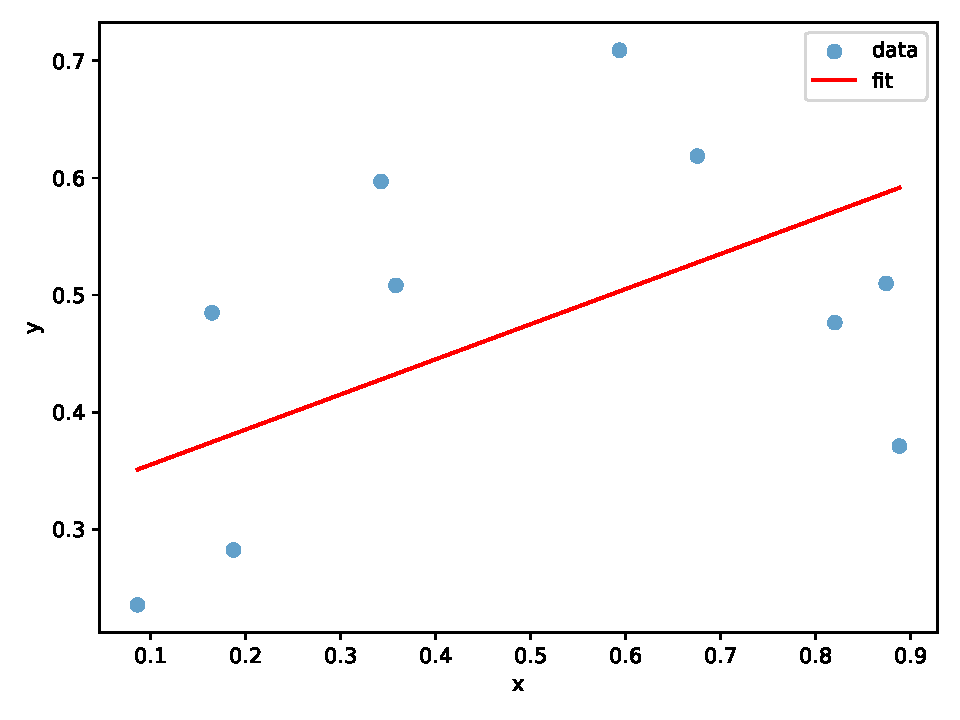
\includegraphics[width=.6\linewidth]{figs/040-lin-plot.pdf}
\caption{Linearna regresija naših začetnih podatkov iz tabele~\ref{t:poly} ne modelira najbolje.}
\end{figure}

Rekli bi lahko, da se te podatke ne da modelirati z linearno regresijo. Ali pač? V tabelo dodajmo nov, izvedeni atribut $x^2$ in naj bo tako dopolnjena tabela vhod za linearno regresijo. Ta bo poiskala uteži atributov za model
%
\begin{margintable}
\begin{tabular}{S S S}
\toprule
{x} & {$x^2$} & {y} \\
\midrule
0.19 & 0.04 & 0.28 \\
0.09 & 0.01 & 0.24 \\
0.16 & 0.03 & 0.48 \\
0.34 & 0.12 & 0.60 \\
0.59 & 0.35 & 0.71 \\
0.87 & 0.76 & 0.51 \\
0.89 & 0.79 & 0.37 \\
0.68 & 0.46 & 0.62 \\
0.36 & 0.13 & 0.51 \\
0.82 & 0.67 & 0.48 \\
\bottomrule
\end{tabular}
\vspace*{3mm}
\caption{Prejšnji tabeli podatkov (tabela~\ref{t:poly}) smo dodali novo kolono oziroma nov atribut, ki smo ga izračunali iz kolone $x$.}
\end{margintable}

\[
y = w_0 + w_1 x + w_2 x^2 .
\]

S tem smo v modelu linearne regresije dodali dodatni atribut. Po obliki naš model sicer ni več linearen v spremenljivki $x$, temveč je kvadraten polinom. Pomembno pa je, da je model še vedno linearen v parametrih ($w_0$, $w_1$, $w_2$), zato lahko zanj uporabimo povsem enak postopek učenja kot prej, torej linearno regresijo. 

Rezultate učenja takega modela lahko znova upodobimo v ravnini $(x,y)$, kot to kaže spodnji graf. Odlično! Model se sedaj dobro prilega učnim podatkom. 
%
\begin{figure}
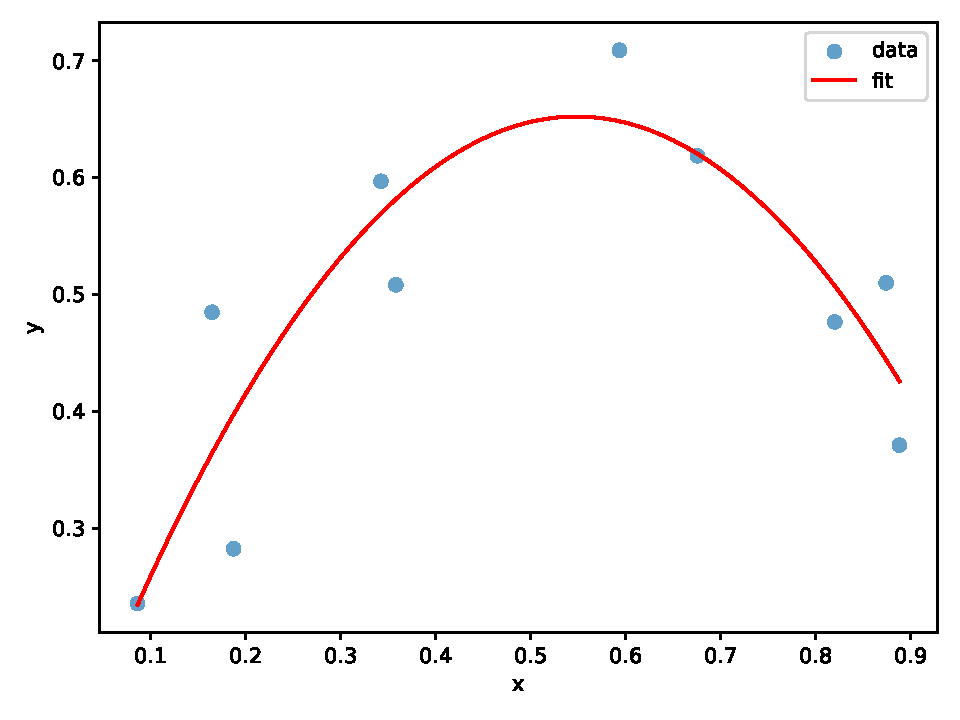
\includegraphics[width=.6\linewidth]{figs/040-poly-plot.pdf}
\caption{Tudi ta model je linearna regresija.}
\end{figure}
%
Tudi vrednost cenovne funkcije, ki jo v linearni regresiji minimiziramo (povprečna vsota kvadratov napak), je veliko manjša kot v primeru, ko v tabelo nismo dodali nove spremenljivke. In sicer se je iz $0.018$ za osnovne podatke zmanjšala na zgolj $0.005$.


Nihče nas sicer ne ovira\marginnote{Tovrstno razširitev učne množice imenujemo {\em polinomska razširitev}, trik, ko to združimo z linearno regresijo pa {\em polinomska regresija}}, da z dodajanjem atributov ne nadaljujemo. Lahko bi namreč dodali še potence višjega reda. Recimo $x^3$, $x^4$, vse do recimo $x^7$. Cenovno funkcijo smo uspeli še malo zmanjšati, tokrat na $0.003$. Uspešno, torej!? 

\begin{figure}
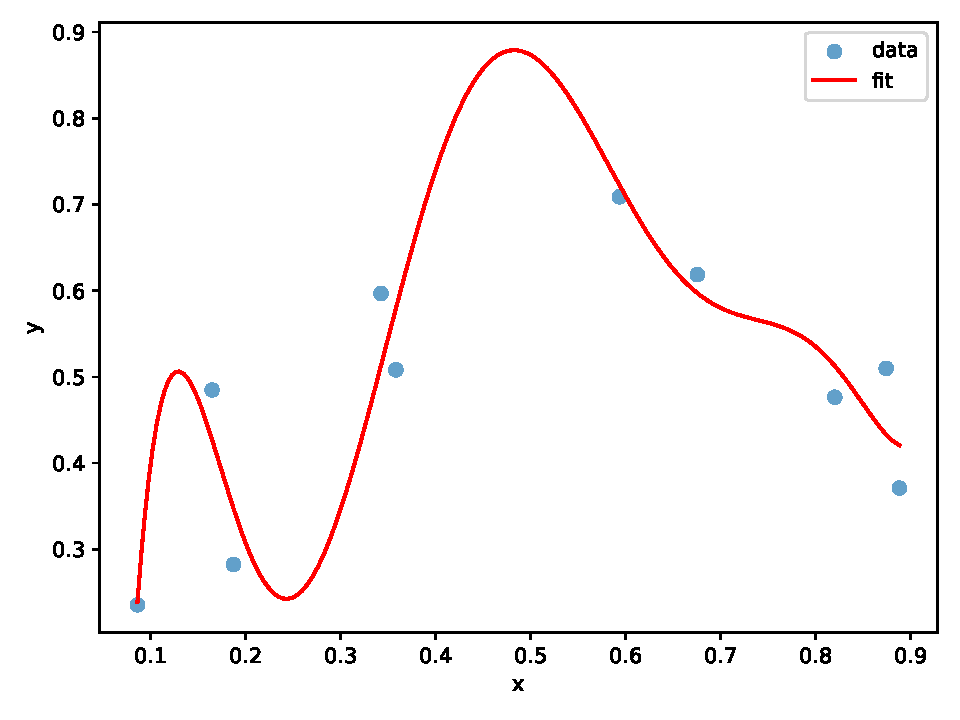
\includegraphics[width=.6\linewidth]{figs/040-poly-plot-7.pdf}
\caption{In tudi to je linearna regresija.}
\end{figure}

Želja po zmanjšanju cenovne funkcije\marginnote{Kaj bi se zgodilo pri dodajanju atributov do polinoma devete stopnje, torej do točke, ko bi vključili tudi $x^9$. Koliko bi bila vrednost kriterijske funkcije takrat? Zakaj?} nas je privedla (skoraj) do ekstrema. Model se je pričel popolnoma prilagajati učni množici in kot tak za napovedovanje ni več uporaben.

\section{Regularizacija L2}

Če si pri zgornjem primeru nekoliko podrobneje ogledamo uteži modela, opazimo zanimiv pojav. Pri modelu druge stopnje so uteži še razmeroma majhne. Ko pa začnemo dodajati nove atribute, torej potence $x^3$, $x^4$, $x^5$ in tako naprej, uteži hitro postanejo zelo velike. Nekatere so pozitivne, druge negativne, njihove absolutne vrednosti pa lahko postanejo tudi več tisočkrat, tudi desettisočkrat večje od vrednosti vhodnih spremenljivk.

To tudi pojasni, zakaj postaja funkcija $y(x)$ oziroma njena odvisnost od vhodne spremenljivke $x$ čedalje bolj zapletena. Velike uteži pomenijo, da lahko že zelo majhna sprememba vhodne spremenljivke $x$ povzroči veliko spremembo v napovedani vrednosti $y$. Model zato začne slediti vsaki malenkostni spremembi v učnih podatkih in s tem pravzaprav modelira tudi šum. Dobljeni model tako sicer zelo dobro prilega učni množici, a postaja za napovedovanje novih primerov neuporaben.

Opazovanje vrednosti uteži pri dodajanju atributov, kot smo jo opazili zgoraj, nas vodi k naslednji ideji. Poleg želje k dobremu prileganju učnim podatkom si pri gradnji linearnega modela lahko zaželimo tudi, da so uteži modela čim manjše ter da je model na ta način enostavnejši. V cenovno funkcijo moramo zato poleg napake modela vključiti še kazen za velike uteži. Ker nas pri tem ne zanima, ali je utež pozitivna ali negativna, uteži kvadriramo. Pri tem običajno izpustimo utež $w_0$, saj ta predstavlja zgolj začetno vrednost funkcije. Cenovna funkcija linearne regresije tako postane
%
\[
J(\mathbf{w}) =
\frac{1}{n} \sum_{i=1}^{n} (y_i - \hat{y}_i)^2
+
\lambda \sum_{j=1}^{p} w_j^2 .
\]

Prvi člen cenovne funkcije je enak temu, ki ga že poznamo, torej povprečni kvadrirani napaki napovedi. Drugi člen pa kaznuje  velike uteži. Ker gre za vsoto dveh členov, ki nista v enakih merskih enotah in tudi konceptualno različna, moramo drugi, novi člen ustrezno utežiti. To storimo s parametrom $\lambda$, ki mu pravimo \emph{stopnja regularizacije}. V implementaciji za regularizacijo torej spremenimo samo izračun funkcije izgube znotraj razreda \texttt{LinReg}, ki implementira linearno regresijo:

\vspace*{3mm}
\begin{lstlisting}
def loss(self, xs, ys):
    yhats = [self(x) for x in xs]
	loss = sum([(y - yhat)**2  for y, yhat in zip(ys, yhats)]) \
	       / Value(len(xs))
    loss += self.reg_strength * sum([w**2 for w in self.weights]) \
            / len(self.weights)
    return loss
\end{lstlisting}
%
Funkcija \texttt{loss} predpostavlja, da smo v razredu primerno inicializirali spremenljivko \texttt{self.reg\_strength}. Regularizacijski člen smo dodatno tudi delili s številom uteži modela, kjer se spomnimo, da sem ni vključenega člena \texttt{self.b}.

Pri stopnji regularizacije $\lambda = 0$ (to je, ko je \texttt{self.reg\_strength} enak 0.0) dobimo natanko isti model kot pri navadni linearni regresiji. Ko vrednost $\lambda$ povečujemo, začne kazen za velike uteži postajati vedno pomembnejša. Model zato raje izbira manjše uteži, posledično pa postaja funkcija $y(x)$ bolj gladka in enostavnejša. Kaj pa se zgodi, če stopnjo regularizacije povečamo na zelo veliko vrednost? V tem primeru drugi člen v cenovni funkciji prevlada in model teži k temu, da so vse uteži čim bližje nič. 

Kolikšna bo v tem primeru vrednost $w_0$? Cenovno funkcijo lahko takrat zapišemo kot
%
\[
J(w_0) = \frac{1}{n} \sum_{i=1}^{n} (y_i - w_0)^2 .
\]
%
Poiščimo minimum te funkcije. Odvajamo po $w_0$:
%
\[
\frac{\partial J}{\partial w_0}
=
\frac{1}{n} \sum_{i=1}^{n} 2(w_0 - y_i).
\]
%
Pri minimumu mora biti odvod enak nič:
%
\[
\sum_{i=1}^{n} (w_0 - y_i) = 0 .
\]
%
Od tod sledi
%
\[
n w_0 = \sum_{i=1}^{n} y_i ,
\]
%
oziroma
%
\[
w_0 = \frac{1}{n} \sum_{i=1}^{n} y_i .
\]

Vidimo torej, da bo model pri zelo veliki stopnji regularizacije napovedoval kar povprečno vrednost učnih podatkov $y$. Kar je silno zanimivo: popolnoma zglajeni model, oziroma najbolje enostaven model, je torej napoved s povprečno vrednostjo.

Postopek\marginnote{Ime izhaja iz oblike optimizacijskega problema: dodatek ($\lambda \sum_j w_j^2$) spremeni površino cenovne funkcije tako, da ima izrazit greben (angl. {\em ridge}) vzdolž smeri, kjer so parametri slabo določeni zaradi močne korelacije med atributi. Regularizacijski člen ta ``greben'' zaobli, zato ima problem enolično rešitev in uteži ostanejo omejene.}, ki smo ga pravkar opisali, imenujemo \emph{regularizacija}. Ker pri tem kvadriramo uteži, govorimo natančneje o \emph{L2 regularizaciji}. Ta pristop je v literaturi pogosto znan tudi kot grebenska regresija (angl. \emph{ridge regression}).

\section{Ocenjevanje točnosti modela z $R^2$}

Pomudimo se še malo pri napovedovanju s povprečno vrednostjo na učni množici. Oziroma, pri najenostavnejšem regresijskem modelu, ki ga torej zgradimo brez upoštevanja vrednosti atributov. Pričakujemo, da bodo modeli, ki bodo upoštevali te vrednosti bolj točni, oziroma da bo njihova napaka manjša. Smiselno bi zato bilo oceniti razmerje med napako, ki jo dobimo pri atributno informiranem modelu in našim osnovnim modelom, kjer napovedujemo s povprečno vrednostjo:

\[
\frac{\sum_{i=1}^{n}(y_i - \hat{y}_i)^2}
{\sum_{i=1}^{n}(y_i - \bar{y})^2},
\]

kjer je $\hat{y}_i$ napoved našega modela, $\bar{y} = \frac{1}{n}\sum_{i=1}^{n} y_i$ pa povprečna vrednost ciljne spremenljivke. Če je vrednost tega količnika blizu $0$, pomeni, da je naš model bistveno boljši od napovedovanja s povprečjem. Če je enaka $1$, je model enako dober kot osnovni model, če pa je večja od $1$, je celo slabši.

Ker si želimo mero, pri kateri večje vrednosti pomenijo boljši model (najbolje blizu $1$) in slabše vrednosti bližje $0$, ta količnik odštejemo od $1$ in dobimo mero $R^2$:

\[
R^2 = 1 - \frac{\sum_{i=1}^{n}(y_i - \hat{y}_i)^2}
{\sum_{i=1}^{n}(y_i - \bar{y})^2}.
\]

Mera $R^2$ je pogosto bolj primerna od mer, kot je RMSE, ker je brezrazsežna in vedno v enakem razponu, torej med 0 in 1\marginpar{Pa je to res? Je možno, da bi kakšen model napovedoval slabše od najenostavnejšega modela? Bo to tako na učni množici primerov ali na novih primerih?}, ter zato omogoča primerjavo točnosti med različnimi podatkovnimi množicami ali problemi. Medtem ko RMSE podaja napako v enotah ciljne spremenljivke, $R^2$ izraža, kolikšen delež variance podatkov pojasni model, kar je pogosto bolj intuitivno. Poleg tega $R^2$ neposredno primerja model z osnovnim pristopom napovedovanja s povprečjem, zato takoj pove, ali model dejansko prinaša izboljšavo.

\section{Regularizacija L1}

Pri L2 regularizaciji smo kaznovali velike uteži tako, da smo v cenovno funkcijo dodali vsoto njihovih kvadratov. Uteži so se zato sicer zmanjšale, vendar praviloma nobena od njih ni postala natanko enaka nič. Model je tako še vedno uporabljal vse atribute, le z nekoliko manjšimi utežmi. Če pa je naš cilj, da bi model nekatere atribute povsem izločil, potrebujemo nekoliko drugačen pristop. Namesto kvadratov uteži lahko v cenovno funkcijo vključimo vsoto njihovih absolutnih vrednosti. Dobimo cenovno funkcijo

\[
J(\mathbf{w}) =
\frac{1}{n} \sum_{i=1}^{n} (y_i - \hat{y}_i)^2
+
\lambda \sum_{j=1}^{p} |w_j|.
\]

Kaj se zgodi, ko povečujemo stopnjo regularizacije $\lambda$? Podobno kot prej začne model raje izbirati manjše uteži. A tokrat se zgodi še nekaj zanimivega: nekatere uteži postanejo natanko enake nič. Tak atribut model dejansko ne uporablja več. Lahko bi rekli, da smo ga iz modela izločili.

Zato ima L1 regularizacija zelo praktično lastnost: poleg omejevanja kompleksnosti modela hkrati opravlja tudi \emph{izbor značilk}. Model sam odloči, katere vhodne spremenljivke so za napoved pomembne in katere lahko mirno zanemari.

Če stopnjo regularizacije še naprej povečujemo, bo uteži, ki so različne od nič, vedno manj. Pri zelo velikih vrednostih $\lambda$ bo na koncu ostala le še utež $w_0$, model pa bo znova postal konstanta, ki napoveduje povprečno vrednost učnih podatkov.

Postopek, ki smo ga pravkar opisali, imenujemo \emph{L1 regularizacija}. V statistični literaturi je znan tudi pod imenom \emph{LASSO} (angl. \emph{Least Absolute Shrinkage and Selection Operator}). Njegova posebnost je prav v tem, da poleg regularizacije omogoča tudi avtomatski izbor atributov, kar je v praksi pogosto zelo uporabno. Implementacija te regularizacije v načelu spet spremeni samo izračun kriterijske funkcije. Spodaj je ta funkcija, ki implementira obe do sedaj omenjeni regularizaciji:

\vspace*{3mm}
\begin{lstlisting}
def loss(self, xs, ys):
    yhats = [self(x) for x in xs]

    loss = sum([(y - yhat)**2  for y, yhat in zip(ys, yhats)]) \
           / Value(len(xs))
    if self.reg == 'l1':
        loss += self.reg_strength * sum([abs(w) for w in self.weights]) \
                / len(self.weights)
    elif self.reg == 'l2':
        loss += self.reg_strength * sum([w**2 for w in self.weights]) \
                / len(self.weights)
    return loss
\end{lstlisting}

Za tipične primere je zgornje dovolj, če pa želimo prehod k ničelnim vrednostim uteži še dodatno spodbuditi, lahko to storimo neposredno v postopku gradientnega sestopa. Po posodobitvi parametrov dodamo še korak, kjer majhne vrednosti uteži postavimo na nič. Intuitivno gledano ta korak ``potisne'' uteži proti nič: če je njihova absolutna vrednost manjša od praga, jih nastavimo na nič. Ta postopek pogosto imenujemo \emph{krčenje} (angl.~\emph{shrinkage}) in še okrepi lastnost L1 regularizacije, da izloča nepomembne atribute.

\vspace*{3mm}
\begin{lstlisting}
if model.reg == 'l1':
    shrink = learning_rate * model.reg_strength
    for p in model.parameters():
        if abs(p.data) < shrink:
            p.data = 0
\end{lstlisting}


\section{Grafična primerjava regularizacij}

Regularizacijo lahko razumemo tudi nekoliko drugače. Namesto da regularizacijski člen dodamo cenovni funkciji, lahko problem zapišemo kot optimizacijo z omejitvijo:

\[
\min_{\mathbf{w}} 
\frac{1}{n}\sum_{i=1}^{n}(y_i-\hat{y}_i)^2
\qquad
\text{pri pogoju}
\qquad
R(\mathbf w) \le s .
\]

Pri tem funkcija $R(\mathbf w)$ določa velikost uteži, parameter $s$ pa omejuje, kako velike te uteži smejo biti.

Če imamo le dve uteži, $w_1$ in $w_2$, lahko ta problem prikažemo v ravnini $(w_1,w_2)$. Izolinije napake (brez regularizacije) so elipse. Rešitev dobimo v točki, kjer se najnižja elipsa prvič dotakne dovoljene množice uteži.

Pri L2 regularizaciji je omejitev

\[
w_1^2 + w_2^2 \le s ,
\]

kar v ravnini predstavlja krog. Dotik z elipso se zato običajno zgodi nekje na gladkem robu kroga, tako da so uteži sicer manjše, vendar praviloma nobena ni natanko enaka nič.

Pri L1 regularizaciji pa omejitev postane

\[
|w_1| + |w_2| \le s ,
\]

kar v ravnini $(w_1,w_2)$ tvori romb. Ker ima romb ostre vogale na koordinatnih oseh, se elipse pogosto dotaknejo prav v enem od teh vogalov. V takšni točki pa je ena od uteži natanko enaka nič.

\section{Regularizacija in točnost na učni in testni množici}

Zaenkrat smo točnost modelov ocenjevali le v postopku optimizacije, kjer smo si, nekoliko naivno, prizadevali, da učne podatke modeliramo čim bolj točno. Regularizacija seveda ta koncept ukine in doda ``potenciometer'', ki pove, kakšno naj bo razmerje med enostavnostjo in točnostjo. Na učni množici bo dvig stopnje regularizacije torej kvaril model s stališča točnosti na učnih podatkih. Kako pa bo regularizacija vplivala na točnost na testnih podatkih?

Opazujmo ta razmerja na poskusu. Množico podaktov o deležu telesne maščobe, ki smo jo uporabili že v prejšnjem poglavju, bomo tokrat razdelili na učne in testne podatke. Da bo vpliv regularizacije izrazitejši~\marginpar{Zakaj bi take delitev podatkov izraziteje pokazala na vpliv regularizacije?}, bomo iz podatkov vzorčili zelo majhno učno množico in vse ostale podatke pustili za testiranje:

\vspace*{3mm}
\begin{lstlisting}
df = pd.read_csv("body-fat-brozek.csv")
feature_names = df.columns[1:].tolist()
ys = df.iloc[:, 0].tolist()
X = df.iloc[:, 1:].values.tolist()

X_arr = np.array(X)
mean = X_arr.mean(axis=0)
std = X_arr.std(axis=0)
X_norm = ((X_arr - mean) / std).tolist()

X_train, X_test, y_train, y_test = 
   train_test_split(X_norm, ys, test_size=0.95, random_state=42)
\end{lstlisting}

Podatke smo, kot je razvidno iz zgornjega, pred učenjem tudi standardizirali. Tovrstna normalizacija podatkov nam omogoča hitrejšo konvergenco gradientnega sestopa, saj so vse značilke na po velikosti primerljive in je prostor optimizacije bolj enakomernen, kar preprečuje cik-cakasto napredovanje in pospeši približevanje minimumu. Sledi poskus, kjer model gradimo pri različnih stopnjah regularizacije in izpisujemo točnost tako na učni kot na testni množici:

\vspace*{3mm}
\begin{lstlisting}
reg_strengths = [0.001, 0.05, 0.01, 0.1, 0.5, 1, 5, 10, 20, 30]
for reg_strength in reg_strengths:
    lr = LinReg(n_inputs=len(feature_names), reg='l1',
                reg_strength=reg_strength)
    model = train(lr, X_train, y_train, n_epochs=1000, 
                  batch_size=None, learning_rate=0.01)
    # print("Weights (most to least important):")
    # print_weights(model, feature_names)

    # evaluate the model on the training and testing sets
    y_pred_train = [model(xi).data for xi in X_train]
    r2_train = r2_score(y_train, y_pred_train)

    y_pred_test = [model(xi).data for xi in X_test]
    r2_test = r2_score(y_test, y_pred_test)

    non_zero_weights = len([w for w in model.weights if w.data != 0])
    print(f"lambda: {reg_strength:5.2f}, R2: {r2_train:.3f} & " \
           "{r2_test:.3f}, non-zero weights: {non_zero_weights}")
\end{lstlisting}

Rezultat kaže monotono padanje točnosti na učni množici pri večanju stopnje regularizacije:
%
\vspace*{3mm}
\begin{lstlisting}
lambda:  0.00, R2: 0.925 & 0.493, non-zero weights: 14
lambda:  0.05, R2: 0.927 & 0.490, non-zero weights: 13
lambda:  0.01, R2: 0.933 & 0.398, non-zero weights: 14
lambda:  0.10, R2: 0.929 & 0.472, non-zero weights: 14
lambda:  0.50, R2: 0.898 & 0.518, non-zero weights: 7
lambda:  1.00, R2: 0.889 & 0.540, non-zero weights: 8
lambda:  5.00, R2: 0.756 & 0.484, non-zero weights: 2
lambda: 10.00, R2: 0.725 & 0.592, non-zero weights: 3
lambda: 20.00, R2: 0.564 & 0.453, non-zero weights: 1
lambda: 30.00, R2: 0.496 & 0.414, non-zero weights: 1
\end{lstlisting}
%
Popolnoma drugače pa je na testni množici, kjer je model najbolj točen pri regularizaciji z $\lambda=10$. Podobno obnašanje bi dobili tudi pri regularizaciji L2, a to in dodatne poskuse prepuščamo bralcu. Postavi pa se vprašanje, kako poiščemo stopnjo regularizacije tako, da bo ta vodila k modelu, ki bo kar najbolj primeren za nove podatke.

\section{Kako poiščemo pravo stopnjo regularizacije}

V bistvu težko in moramo pri tem biti zelo previdni, še posebej ker želimo poročati tako o ``pravi'' stopnji regularizacije kot tudi o oceni točnosti tako dobljenega modela. Tu bomo predpostavili, da iščemo stopnjo regularizacije tako, da to izbiramo iz nekega seznama in gledamo, kdaj naš model dosega najbolši rezultat na neki ločeni množici. Tako kot smo to storili v prejšnjem razdelku. Tam smo najbolši model dobili pri $\lambda=10$, njegova točnost na učni množici je bila $R^2=0.592$. Torej izberemo tako zgrajeni model in napovemo, da bo njegova točnost na novih primerih predvidoma $R^2=0.592$?

Ne. Ta ocena je pristranska, saj smo stopnjo regularizacije izbrali prav na podlagi testne množice, ki je bila s tem ``porabljena'' za učenje. Takšna ocena točnosti je zato preveč optimistična in ne odraža dejanske uspešnosti modela na novih podatkih.

Nadvse pomembno: učenje tokrat ni samo gradnja linearnega modela, ampak vključuje tudi izbor primerne stopnje regularizacije. Vse to skupaj moramo torej preveriti in točnost oceniti na neodvisni testni množici.

Da bi se torej pristranosti pri oceni točnosti izognili, moramo podatke razdeliti še na dodatno testno množico. Podatke bomo torej razdelili na tri disjunktne množice:
\begin{enumerate}
    \item \textbf{učna množica} (recimo 70\% podatkov), na kateri model, pri dani stopnji regularizacije naučimo,
    \item \textbf{validacijska množica} (npr. 15\%), na kateri opazujemo točnost modela pri dani stopnji regularizacije in ki nam omogoča izbor primerne stopnje, torej tiste, pri kateri je na validacijski množici regulariziran model najbolj točen,
    \item \textbf{testna množica} (npr. 15\%), na kateri na koncu ocenimo točnost modela.
\end{enumerate}

O katerem modelu potem poročamo? Tistemu, ki je bil na validacijski množici najboljši? Ne. Tak model je bil naučen le na učni množici in zato ne izkorišča vseh razpoložljivih podatkov. Za gradnjo končnega modela spet izhajamo iz vseh podatkov, te tokrat delimo samo na učno in validacijsko množico, ponovimo celotni postopek izbora stopnje regulacije in poročamo o modelu, ki je dal najboljši rezultat na valicijski množici.

Delitev na učno in valicijsko množico pri zadnjem koraku je potrebna zato, ker naš postopek gradnje modela temelji na taki delitvi. Da ponovimo: postopek gradnje našega modela tokrat ni samo linearna regresija, ampak vključuje tudi korake izbora stopnje regularizacije. Model, ki ga na koncu želimo uporabljati oziroma o katerem bomo poročali torej ni samo rezultat ene optimizacije, ampak rezultat celotnega postopka, ki vključuje tudi izbor stopnje regularizacije. Ta postopek pa po definiciji potrebuje delitev na učno in validacijsko množico.

Za konec, opišimo zgoraj predlagani postopek s pseudokodo:

\vspace*{3mm}
\begin{lstlisting}
# accuracy estimation
split data to train, validation, test
for reg in lambdas:
    model = fit(train, reg)
    score[reg] = evaluate(model, validation)
choose best reg
score = evaluate(fit(train, best_reg), test)

# derivation of final model
split data to train, validation
for reg in lambdas:
    model = fit(train, reg)
    score[reg] = evaluate(model, validation)
choose best reg
model = fit(train, best_reg)
\end{lstlisting}

Kar komplicirano je že zdaj. Je pa tu še en problem. Zgornje je namreč primerno za res velike podatke, pri manjših pa bo sama razdelitev na podmnožice lahko zelo vplivala na oceno točnosti. Pri slednji bi si lahko pomagali s prečnim preverjanjem, in podali oceno tako, da bi bila ta povprečje več eksperimentov. Bi znali zgornje spremeniti na ustrezen način in vključiti prečno preverjanje?




\chapter{Glavne komponente}

V prejšnjih dveh poglavjih smo spoznavali neposredne koristi pristopa k analizi podatkov, kjer za dani model in kriterijsko funkcijo uporabimo strojno odvajanje in gradientni sestop in potem uživamo v rezultatih. Model je bil v prejšnjih dveh poglavjih isti in silno enostaven. Linearna regresija ima prednost, da je model berljiv in podan z utežmi, z uporabo enostavnega trika, regularizacije, pa ga lahko še dodatno zgladimo (regularizacija L2) ali pa poenostavimo (regularizacija L1).

Lahko podoben pristop uporabimo za nek popolnoma drugačen model? Tu ne mislimo na napovedne modele, ampak, na primer, na model projekcije ali pa vložitve podatkov. Lahko, ampak da ne prehitevamo: v tem in naslednjem poglavju bo govora o zmanjšanju dimenzij. Tu, v tem poglavju, z iskanjem projekcij, v naslednjem pa z vložitvami. A začnimo na začetku, s primerom in motivacijo.

\section{Razpršenost in varianca}

Prikazana sta dva primera dvodimenzionalnih podatkov. Pri obeh primerih smo podatke standardizirali. Pri prvem so podatki razpršeni po vsem podatkovnem prostoru, pri drugem imajo strukturo, saj sta atributa korelirana, njuna kovarianca je -0.9.

\begin{figure}
    \centering
    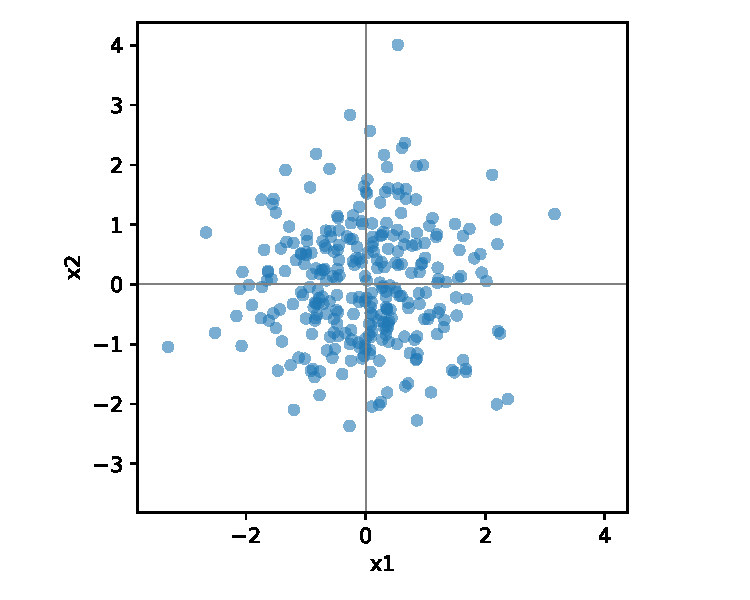
\includegraphics[width=0.48\linewidth]{figs/050-scatter-cor-zero.pdf}\hfill
    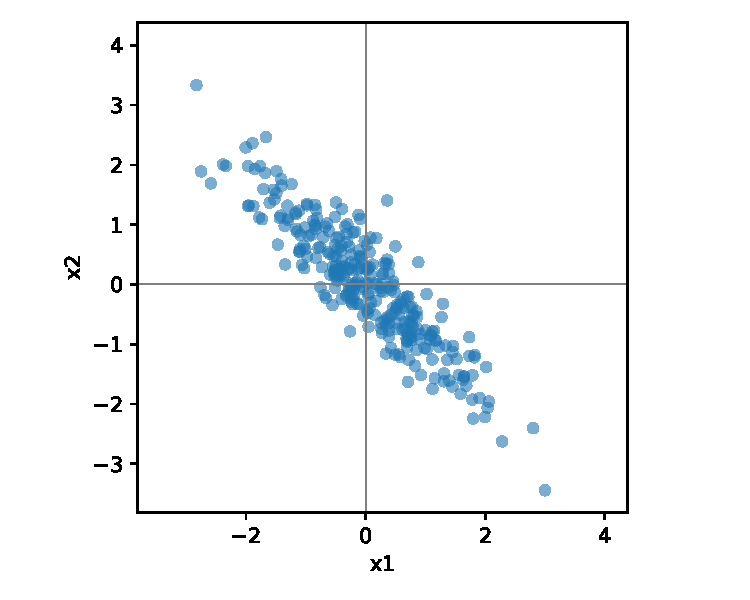
\includegraphics[width=0.48\linewidth]{figs/050-scatter-cor-high.pdf}
    \caption{Dva primera standardiziranih podatkov, prvi (levo) s kovarianco $0$ in drugi s kovarianco $-0,9$.}
    \label{fig:data}
\end{figure}

Pri generiranju dvodimenzionalnih normalno porazdeljenih podatkov z določeno kovarianco nam je pomagal \texttt{numpy}:
\vspace*{3mm}
\begin{lstlisting}
def generate_2d_normal(n, rho, rnd_seed=42):
    np.random.seed(rnd_seed)
    cov = np.array([[1.0, rho], [rho, 1.0]])
    data = np.random.multivariate_normal(mean=[0, 0], cov=cov, size=n)
    mean = data.mean(axis=0)
    std = data.std(axis=0)
    return (data - mean) / std
\end{lstlisting}

Želeli bi ugotoviti, v kateri smeri se podatki raztezajo, oziroma katera je smer, kjer so podatki najbolj razpršeni. Za naš primer s kovarianco $-0.9$ spodaj sta prikazani dve taki smeri, podani z dvema smernima vektorjema $a$ in $b$. 

\begin{figure}
    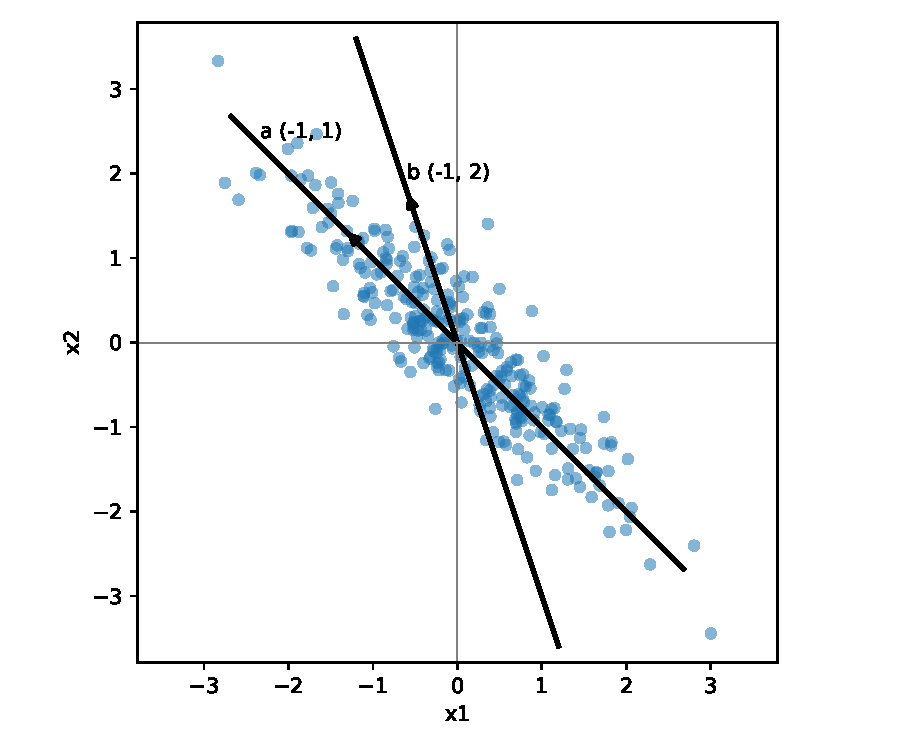
\includegraphics[width=0.5\textwidth]{figs/050-two-directions.pdf}
    \caption{Dve kandidatni smeri, po katerih lahko opazujemo razpršenost podatkov.}
    \label{fig:ab}
\end{figure}

Očitno so podatki bolj razpršeni v smeri vektorja $a$. A kako to pokažemo matematično? Razpršenost v statistiki merimo z varianco. Za enodimenzionalne podatke $z_1,\dots,z_n$ je varianca definirana kot
$$
\mathrm{Var}(z)=\frac{1}{n}\sum_{i=1}^n (z_i-\bar z)^2.
$$

Če želimo meriti razpršenost v določeni smeri, podatke projiciramo na enotni smerni vektor $u$, kjer velja $|u|=1$. Vektor $u$ izberemo kot smer v prostoru (npr. kandidatna smer $a$ ali $b$), ki jo želimo analizirati. Za smer $a$ bo smerni vektor $u=\frac{a}{|a|}$.

Naj bodo podatki zapisani v matriki $X\in\mathbb{R}^{n\times d}$, kjer vsaka vrstica predstavlja en primer. Ker so naši podatki dvodimenzionalni, ima matrika $X$ dve koloni. Projekcija podatkov na smer $u$ je potem podana kot
$$
X_u = X u,
$$
kjer $X_u\in\mathbb{R}^n$ predstavlja (enodimenzionalno) projekcijo naših podatkov. Smerni vektor\marginnote{Znova smo pri linearni kombinaciji atributov! Tudi tu ponovno srečamo uteži. Vodi to k interpretaciji rezultatov?} $u$ tudi določa uteži vhodnih atributov in torej njihovo linearno kombinacijo.

Za oba naša smerna vektorja lahko sedaj ugotovimo, kakšna je varianca, če podatke projiciramo na smeri, ki jih določata:
\vspace*{3mm}
\begin{lstlisting}
X = generate_2d_normal(n, rho=rho)
a = np.array([-1.0, 1.0])
b = np.array([-1.0, 3.0])
for v in [a, b]:
    var = projected_variance(X, v)
    print(f"Projected variance along ({v[0]}, {v[1]}): {var:.3f}")
\end{lstlisting}

Rezultat je pričakovan, podatki na projekciji na vektor $a$ so bolj razpršeni:
\vspace*{3mm}
\begin{lstlisting}
Projected variance along (-1.0, 1.0): 1.902
Projected variance along (-1.0, 3.0): 1.541
\end{lstlisting}

Lahko smerni vektor projekcije, kjer bi bili podatki najbolj razpršeni, poiščemo algoritmično? Lahko. Postopek se imenuje analiza glavnih komponent in jo bralec najbrž pozna, a bi jo tu (seveda) radi izvedli z gradientnim sestopom in z uporabo strojnega odvajanja.

\section{Iskanje glavne komponente}

Naj bo torej $u$ smer, na katero projiciramo podatke. Iščemo $u$, kjer so podatki najbolj razpršeni, torej kjer je varianca projekcije največja. Najprej zapišimo varianco projiciranih podatkov:
$$
\mathrm{Var}(X_u)=\frac{1}{n}\sum_{i=1}^n (x_i^\top u)^2,
$$
kjer smo upoštevali, da so podatki standardizirani in centrirani, zato je povprečje projekcije enako $0$. To lahko zapišemo v matrični obliki\marginnote{Pri tem zapisu smo si pomagali z dejstvom, da, če je $z$ skalar, velja $z=z\top$. Kako nam to pomaga?} kot
$$
\mathrm{Var}(X_u)=\frac{1}{n} u^\top X^\top X u.
$$

Določimo kriterijsko funkcijo
$$
J(u)=\frac{1}{n} u^\top X^\top X u,
$$
ki meri razpršenost podatkov v smeri $u$. Iščemo tak $u$, ki maksimizira $J(u)$, ob pogoju $|u|=1$. Tako dobimo optimizacijski problem
$$
\max_u J(u) \quad \text{pri pogoju} \quad |u|=1,
$$
ki ga lahko rešujemo z gradientnim sestopom (oziroma vzponom), pri čemer bomo morali po vsakem koraku vektor, ki osveži elemente vektorja $u$, ta vektor normirati, da zagotovimo, da ostane enoten.

Opisano funkcionalnost\marginnote{Malo nevšečno je, da moramo zato med parametre funkcije izgube vključiti \texttt{ys}, a spremembe funkcije \texttt{train}, ki bi omogočala klice brez \texttt{ys} in hkrati omogočala optimizacijo za linearno regresijo in iskanje glavne komponente prepuščamo bralcu.} implementirajmo v razredu \texttt{PCA1D}. Pri tem skušamo slediti strukturi implementacije linearne regresije, tako da ne spreminjamo ničesar v naši implementaciji gradientnega sestopa oziroma v funkciji \texttt{train}.

\vspace*{3mm}
\begin{lstlisting}
class PCA1D:
    def __init__(self, n_inputs, rnd_seed=42):
        rng = random.Random(rnd_seed)
        self.u = [Value(rng.uniform(-1, 1), label=f"u{i}") \
                  for i in range(n_inputs)]
        self.normalize_u()

    def parameters(self):
        return self.u

    def _dot(self, a, b):
        return sum(ai * bi for ai, bi in zip(a, b))

    def normalize_u(self, eps=1e-8):
        nrm = (self._dot(self.u, self.u) + eps) ** 0.5
        self.u = [ui / nrm for ui in self.u]

    def loss(self, xs, ys=None):
        self.normalize_u()
        total = Value(0.0, label="proj_var_sum")
        for x in xs:
            z = self._dot(x, self.u)
            total += z**2
        variance = total / len(xs)
        return -variance

    def batch_loss(self, xs, ys=None, m=20):
        indices = random.sample(range(len(xs)), m)
        batch_xs = [xs[idx] for idx in indices]
        return self.loss(batch_xs, ys=None)

    def explained_variance(self, xs):
        return -self.loss(xs, ys=None).data

    def __repr__(self):
        self.normalize_u()
        return "PCA1D(u=[" + \
               ", ".join(f"{ui.data:.3f}" for ui in self.u) + "])"
\end{lstlisting}

V kodi smo kriterijsko funkcijo obrnili v izgubo tako, da minimiziramo $-J(u)$ namesto da bi maksimizirali $J(u)$. To nam omogoča, da brez sprememb uporabimo isti postopek učenja kot prej. Ker mora biti $u$ enotni smerni vektor, ga v funkciji \texttt{normalize\_u} po vsakem osveževanju normiramo. Metoda \texttt{loss} tako izračuna negativno varianco projekcij podatkov na smer $u$, gradientni sestop pa naj bi nato poiskal smer, v kateri je ta varianca največja.

Uporabimo sedaj našo zgornjo implementacijo:

\vspace*{3mm}
\begin{lstlisting}
X = generate_2d_normal(n, rho=rho)
pca = PCA1D(n_inputs=X.shape[1], rnd_seed=42)
train(pca, X, None, learning_rate=0.05, n_epochs=50, report_every=5, batch_size=None)
pca.normalize_u()

var = -pca.loss(X, ys=None).data
print(f"u: [{', '.join(f'{ui.data:.3f}' for ui in pca.u)}]")
print(f"variance: {var:.3f}")
\end{lstlisting}

Naš primer podatkov je očitno precej enostaven, zato postopek iskanja glavne komponente hitro konvergira:
%
\vspace*{3mm}
\begin{lstlisting}
   5 Loss: -1.769 PCA1D(u=[0.523, -0.853])
  10 Loss: -1.875 PCA1D(u=[0.629, -0.777])
  15 Loss: -1.897 PCA1D(u=[0.674, -0.739])
  20 Loss: -1.901 PCA1D(u=[0.693, -0.721])
  25 Loss: -1.902 PCA1D(u=[0.701, -0.713])
  30 Loss: -1.902 PCA1D(u=[0.704, -0.710])
  35 Loss: -1.902 PCA1D(u=[0.706, -0.708])
  40 Loss: -1.902 PCA1D(u=[0.707, -0.708])
  45 Loss: -1.902 PCA1D(u=[0.707, -0.707])
  50 Loss: -1.902 PCA1D(u=[0.707, -0.707])
u: [0.707, -0.707]
variance: 1.902
\end{lstlisting}
%
Smerni vektor glavne komponente sovpada s smernim vektorjem $a$ na sliki~\ref{fig:ab} in tudi izračunana varianca podatkov je enaka. 

Vektor $u$ imenujemo \emph{glavna komponenta}, ker določa tisto smer v prostoru podatkov, vzdolž katere je razpršenost projekcij največja, torej smer, ki iz podatkov zajame največ informacije v smislu variance. Beseda ``komponenta'' tu poudari, da gre za novo os oziroma novo koordinato, ki jo sestavimo kot linearno kombinacijo izvornih atributov, beseda ``glavna'' pa, da je med vsemi možnimi smermi prav ta najpomembnejša. Prav na odkrivanju takih, glavnih komponent gradi istoimenska tehnika, a tja še pridemo.

\section{Primer uporabe}

Je tako enostavna metoda sploh uporabna? Je. Kdo pravi, da jo moramo uporabiti samo na sintetičnih dvodimenzionalnih podatkih? Ilustrirajmo njeno uporabo na malo bolj kompleksnem primeru. Zbrali smo podatke o hibridnih avtomobilih in bi jih radi, morda zaradi preglednosti, nekako uredili na enodimenzionalni osi. Vzorec podatkov kaže tabela~\ref{t:cars}, v učno množico pa smo sicer vključili 15 avtomobilov.

\begin{table}[ht]
\centering
\small
\begin{tabular}{lccccc}
\toprule
\textbf{Car} & \textbf{Type} & \textbf{kWh/100 km} & \textbf{HP} & \textbf{0--100 km/h (s)} & \textbf{Trunk (L)} \\
\midrule
Toyota Yaris Hybrid        & 0  & 18 & 116 & 9.7 & 286 \\
Nissan Qashqai e-POWER     & 0  & 21 & 190 & 7.9 & 504 \\
Lexus NX 450h+             & 1  & 24 & 309 & 6.3 & 520 \\
Renault Clio E-Tech Hybrid & 0  & 18 & 145 & 9.9 & 301 \\
Volkswagen Golf eHybrid    & 1  & 21 & 204 & 7.4 & 273 \\
\bottomrule
\end{tabular}
\caption{Podatki z vzorcem sodobnih hibridnih vozil z zmogljivostnimi in uporabnimi značilnostmi. Tip 0 so hibridi, 1 pa priključni hibridi.}
\label{t:cars}
\end{table}

Podatke preberemo, si zapomnimo imena avtomobilov, podatke standardiziramo in izračunamo glavno komponento.

\vspace*{3mm}
\begin{lstlisting}
df = pd.read_excel("cars.xlsx")
labels = df.iloc[:, 0].astype(str).to_list()
feat_names = df.columns[1:].to_list()
X = df.iloc[:, 1:].astype(float).to_numpy()
X = (X - X.mean(axis=0)) / X.std(axis=0)

pca = PCA1D(n_inputs=X.shape[1], rnd_seed=42)
train(pca, X, None, learning_rate=0.05, n_epochs=30, report_every=5, batch_size=None)
pca.normalize_u()
\end{lstlisting}

Konvergenca je tudi tu hitra, gradientni sestop najde rešitev v nekaj deset korakih. Na koncu izračunamo še varianco projekcij, uteži atributov (angl. \texttt{loadings}) ter projekcije posameznih avtomobilov na glavno komponento (angl. \texttt{scores}).

\vspace*{3mm}
\begin{lstlisting}
var = -pca.loss(X, ys=None).data
loadings = sorted(((n, u.data) for n, u in zip(feat_names, pca.u)), key=lambda t: abs(t[1]), reverse=True)
scores = X @ np.array([u.data for u in pca.u])
\end{lstlisting}

Pozicijo avtomobilov na linearni osi lahko sedaj izrišemo:

\begin{figure*}
    \centering
    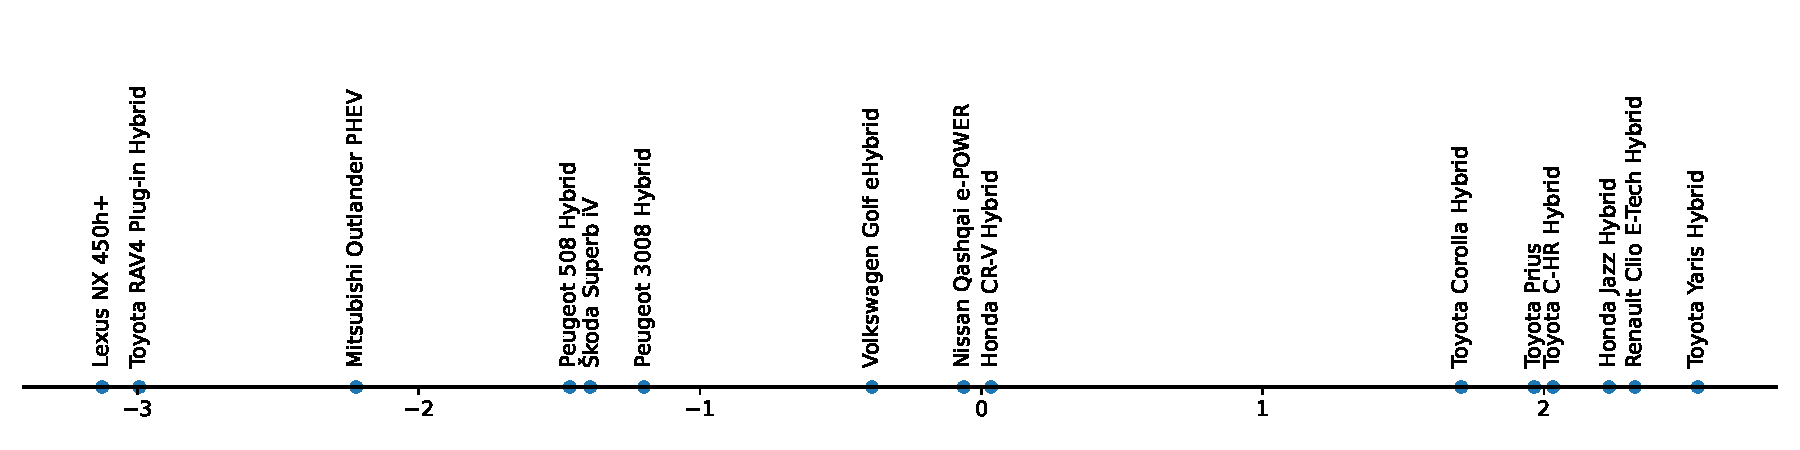
\includegraphics[width=\linewidth]{figs/050-cars.pdf}
    \caption{Rangiranje avtomobilov z metodo glavne komponente.}
    \label{fig:cars-rank}
\end{figure*}

Avtomobili v našem majhnem podatkovnem naboru razpadejo na nekaj skupin. Na desni so manjši, bolj ekonomični avtomobili, na levi pa bolj napredni, večji in najbrž tudi precej dražji. Cena ni bila vključena v tabelo, dodatno interpretacijo rezultatov pa predajamo bralcu. A očitno je, da je tudi tako preprosta tehnika in vizualizacija njenih rezultatov koristna in nudi številne možnosti njene interpretacije. Seveda bi nas pri interpretaciji zanimalo tudi, kakšen je vpliv posameznih atributov, oziroma kakšne so njihove uteži (angl. {\em loadings}). Tu so:

\vspace*{3mm}
\begin{lstlisting}
-0.501: Horsepower
-0.476: kWh/100 km
 0.454: 0-100 km/h (s)
-0.449: Type
-0.339: Trunk Size (L)
\end{lstlisting}

Največji vpliv ima moč motorja (\texttt{horsepower}), tesno ji sledi poraba električne energije (\texttt{kWh/100 km}), nato pa še pospešek, tip pogona in velikost prtljažnika. Negativni predznaki pri moči, porabi in tipu nakazujejo, da večji, zmogljivejši in praviloma priključni hibridi ležijo na enem koncu osi, medtem ko pozitivni prispevek časa pospeška pomeni, da počasnejši, manj zmogljivi avtomobili ležijo na drugem. Glavna komponenta tako v veliki meri pojasni prehod od manjših, manj zmogljivih in varčnejših vozil k večjim, zmogljivejšim in energijsko zahtevnejšim.

\section{Varianca v večrazsežnih prostorih}

Doslej smo razpršenost podatkov merili v eni dimenziji, kjer je varianca določena kot povprečje kvadratov odklonov od centra podatkov. Kako pa merimo razpršenost, kadar so podatki večrazsežni? Naj bodo podatki $x_1, \dots, x_n \in \mathbb{R}^d$. Predpostavimo, da so centrirani, torej $\bar{x} = 0$. Naravna posplošitev variance v večrazsežnem prostoru je
\[
\mathrm{Var}(X) = \frac{1}{n} \sum_{i=1}^n \|x_i\|^2,
\]
kjer $\|x_i\|$ označuje evklidsko normo vektorja $x_i$. Ta definicija ima smisel le, če predpostavimo, da je prostor $\mathbb{R}^d$ evklidski, torej opremljen z evklidsko geometrijo in z običajnim skalarnim produktom
\[
x^\top y = \sum_{j=1}^d x_j y_j,
\]
in pripadajočo normo $\|x\|^2 = x^\top x$. V takem prostoru veljajo znani geometrijski zakoni, med drugim Pitagorov izrek.

\medskip

\textbf{Trditev.} Če so podatki zapisani po koordinatah $x_i = (x_{i1}, \dots, x_{id})$, potem velja
\[
\mathrm{Var}(X) = \sum_{j=1}^d \mathrm{Var}(X^{(j)}),
\]
kjer $X^{(j)}$ označuje $j$-to koordinato podatkov.

\medskip

\textbf{Dokaz.} Začnimo z definicijo večrazsežne variance:
\[
\mathrm{Var}(X) = \frac{1}{n} \sum_{i=1}^n \|x_i\|^2.
\]
Ker uporabljamo evklidsko normo, lahko kvadrat norme razpišemo po koordinatah:
\[
\|x_i\|^2 = \sum_{j=1}^d x_{ij}^2.
\]
Vstavimo:
\[
\mathrm{Var}(X) = \frac{1}{n} \sum_{i=1}^n \sum_{j=1}^d x_{ij}^2.
\]
Zamenjamo vrstni red seštevanja:
\[
\mathrm{Var}(X) = \sum_{j=1}^d \left( \frac{1}{n} \sum_{i=1}^n x_{ij}^2 \right).
\]
Izraz v oklepaju pa je natanko varianca $j$-te koordinate:
\[
\mathrm{Var}(X^{(j)}) = \frac{1}{n} \sum_{i=1}^n x_{ij}^2.
\]
S tem dobimo
\[
\mathrm{Var}(X) = \sum_{j=1}^d \mathrm{Var}(X^{(j)}).
\]
\hfill $\square$

\medskip

Rezultat pove, da se v evklidskem prostoru skupna razpršenost podatkov razstavi na prispevke posameznih koordinat. To je neposredna posledica Pitagorovega izreka: kvadrat dolžine vektorja je vsota kvadratov njegovih projekcij na ortogonalne osi.

Ker se variance
%
\marginnote{Delež razložene variance (angl.~\emph{explained variance}) pove, kolikšen del celotne variance podatkov zajamemo z izbrano projekcijo. Če je skupna varianca podatkov $\mathrm{Var}(X)$, varianca projekcije na smer $u$ pa $\mathrm{Var}(Xu)$, potem je delež razložene variance enak $\mathrm{Var}(Xu) / \mathrm{Var}(X)$. Ta količina meri, koliko informacije (v smislu razpršenosti) ohranimo po projekciji.}
%
seštevajo po oseh, in ker so bili podatki na sliki~\ref{fig:data} standardizirani, lahko zaključimo, da je skupna varianca obeh teh podatkovnih naborov enaka 2. Projekcije na smer $a$ s slike~\ref{fig:ab} potem razložijo $1,902/2,0=95\%$ variance v podatkih, te na smer $b$ pa samo $1,541/2,0=77\%$. Z {\em razložijo} smo mislili, kolikšen delež celotne razpršenosti podatkov zajamemo, če podatke predstavimo le z njihovo projekcijo na izbrano smer. 

\section{Analiza glavnih komponent}

Zgornja lastnost, to je, da lahko v evklidskem prostoru skupno varianco razstavimo na vsoto varianc po posameznih koordinatnih oseh, je ključna tudi za razumevanje analize glavnih komponent. Cilj je poiskati nov koordinatni sistem, kjer so osi med seboj ortogonalne, in kjer se bo skupna varianca ponovno razdelila na vsoto varianc po teh novih oseh. Metoda glavnih komponent je tehnika, kjer izbere tak koordinatni sistem, kjer je večina variance zbrana v čim manjšem številu osi, tako da prva os zajame največji možni delež variance, druga os največji možni delež preostale variance, in tako naprej.

Analizo glavnih komponent 
%
\marginnote{Analizo glavnih komponent (PCA) je uvedel Karl Pearson leta 1901 kot nadaljevanje svojega dela na področju korelacij in kovariančne strukture podatkov, kjer je iskal načine za opis večrazsežnih podatkov z manjšim številom spremenljivk. Harold Hotelling pa je metodo v 1930-ih sistematiziral, uvedel njeno ime ter jo formalno povezal z lastnim razcepom kovariančne matrike in zaporednim iskanjem ortogonalnih komponent.}
%
(angl. PCA, {\em principal component analysis}) mnogokrat uporabimo za iskanje dvodimenzionalne projekcije, saj lahko podatke nato prikažemo v razsevnem diagramu. Naš razred \texttt{PCA1D} lahko razširimo v razred \texttt{PCA2D}, kjer istočasno iščemo dva smerna vektorja $u_1$ in $u_2$, ki sta enotska, med seboj pravokotna, in določata smeri največje skupne variance projekcij. Pri tem mora postopek zagotoviti, da $u_1$ zajame največjo varianco, $u_2$ pa največjo varianco med vsemi smermi, ki so ortogonalne na $u_1$.

Pri tem velja opozoriti, da optimizacija vsote varianc po dveh ortogonalnih smereh določi dvodimenzionalni podprostor največje razložene variance. Posamezni komponenti znotraj tega podprostora pa nista nujno enolično določeni, razen če dodatno zahtevamo, da je prva smer tista z največjo varianco, druga pa pravokotna nanjo in med takimi najbolj variabilna.

Da ohranimo ortogonalnost med vektorjema med optimizacijo, uporabimo Gram--Schmidtovo ortogonalizacijo. Najprej predpostavimo, da imamo dva vektorja $v_1$ in $v_2$, ki ju želimo pretvoriti v ortonormiran par $u_1, u_2$. Postopek poteka v dveh korakih, in sicer z normalizacijo prvega vektorja:
\[
u_1 = \frac{v_1}{\|v_1\|}.
\]
%
in odštevanje projekcije in normalizacija drugega vektorja, kjer najprej iz $v_2$ odstranimo komponento v smeri $u_1$,
\[
\tilde{v}_2 = v_2 - (v_2^\top u_1)\, u_1,
\]
% nato pa dobljeni vektor normiramo:
\[
u_2 = \frac{\tilde{v}_2}{\|\tilde{v}_2\|}.
\]
%
S tem zagotovimo, da velja $u_1^\top u_2 = 0$ in $\|u_1\| = \|u_2\| = 1$. Intuitivno drugi vektor ``očistimo'' komponente v smeri prvega, kar je neposredna posledica Pitagorovega izreka: preostanek leži v pravokotni smeri.


Naša implementacija sledi tej, ki smo jo uporabili za razred \texttt{PCA1D}:
\vspace*{3mm}
\begin{lstlisting}
class PCA2D:
    def __init__(self, n_inputs, rnd_seed=42):
        rng = random.Random(rnd_seed)
        self.v1 = [Value(rng.uniform(-1, 1), label=f"v1_{i}") for i in range(n_inputs)]
        self.v2 = [Value(rng.uniform(-1, 1), label=f"v2_{i}") for i in range(n_inputs)]

    def parameters(self):
        return self.v1 + self.v2

    def _dot(self, a, b):
        return sum(ai * bi for ai, bi in zip(a, b))

    def _norm(self, v, eps=1e-8):
        return (self._dot(v, v) + eps) ** 0.5

    def orthonormal_basis(self):
        # Gram-Schmidt orthonormalization
        nrm1 = self._norm(self.v1)
        u1 = [vi / nrm1 for vi in self.v1]

        proj_v2_on_u1 = self._dot(self.v2, u1)
        v2_orth = [v2i - proj_v2_on_u1 * u1i for v2i, u1i in zip(self.v2, u1)]
        nrm2 = self._norm(v2_orth)
        u2 = [v / nrm2 for v in v2_orth]
        return u1, u2

    def loss(self, xs, ys=None):
        # Maximize projected variance on two orthonormal axes.
        u1, u2 = self.orthonormal_basis()
        total = Value(0.0, label="proj_var_sum_2d")
        for x in xs:
            z1 = self._dot(x, u1)
            z2 = self._dot(x, u2)
            total += z1**2 + z2**2
        explained_var = total / len(xs)
        return -explained_var

    def batch_loss(self, xs, ys=None, m=20):
        indices = random.sample(range(len(xs)), m)
        batch_xs = [xs[idx] for idx in indices]
        return self.loss(batch_xs, ys=None)
\end{lstlisting}

V primerjavi z razredom \texttt{PCA1D} je ključna razlika ta, da tukaj optimiziramo dva smerna vektorja hkrati. Namesto enega vektorja $u$ imamo dva kandidata $v_1$ in $v_2$, ki ju med vsakim izračunom pretvorimo v ortonormirano bazo $(u_1, u_2)$ z Gram--Schmidtovim postopkom. Funkcija izgube tako ne meri več variance projekcije na eno smer, temveč vsoto varianc projekcij na obe smeri. S tem zajamemo skupno razpršenost podatkov v dvodimenzionalni podprostor. Pomembno je tudi, da ortogonalizacijo izvajamo sproti (znotraj metode \texttt{orthonormal\_basis}), zato ni treba eksplicitno omejevati parametrov — pogoj pravokotnosti in enotske dolžine je zagotovljen konstrukcijsko. Tako razširjena metoda dejansko išče prvi dve glavni komponenti hkrati.

Program tudi tu konvergira hitro. V namene analize izpišemo deleže razložene variance
%
\vspace*{3mm}
\begin{lstlisting}
Total variance: 5.000
Explained variance (PC1): 2.413 (48.3%)
Explained variance (PC2): 2.102 (42.0%)
Total explained variance (PC1+PC2): 4.515 (90.3%)
\end{lstlisting}
%
ter pojasnimo sestavo posameznih komponent,
\vspace*{3mm}
\begin{lstlisting}
Loadings, PC1:
 -0.630: Type
  0.444: 0-100 km/h (s)
 -0.392: Horsepower
 -0.370: kWh/100 km
  0.339: Trunk Size (L)

Loadings, PC2:
 -0.881: Trunk Size (L)
 -0.313: Horsepower
 -0.299: kWh/100 km
  0.187: 0-100 km/h (s)
  0.028: Type
\end{lstlisting}
% 
ter te uporabimo pri interpretaciji dobljene projekcije.

\begin{figure}
    \centering
    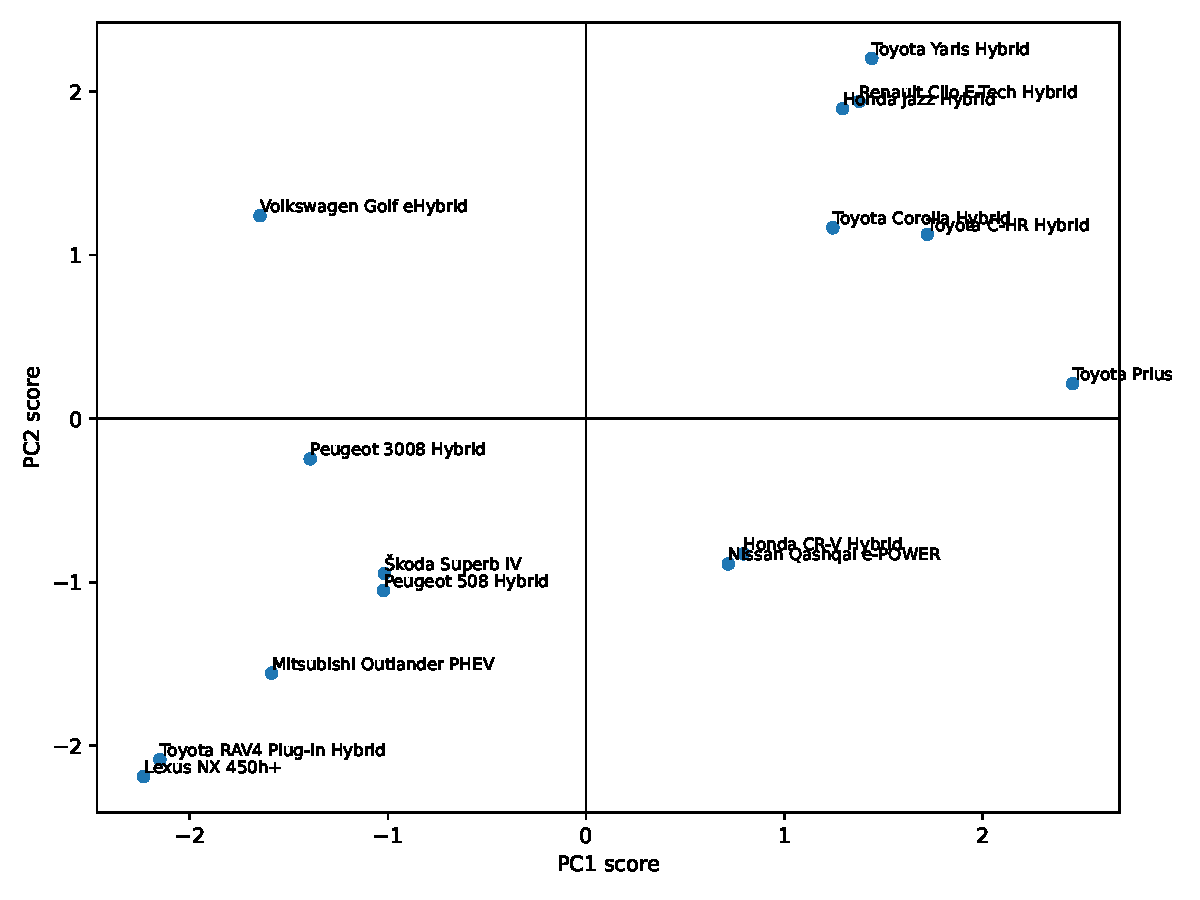
\includegraphics[width=\linewidth]{figs/050-cars-2d.pdf}
    \caption{Dvodimenzionalna projekcija podatkov o avtomobilih.}
    \label{fig:cars-2d}
\end{figure}

Prvi dve glavni komponenti torej zajameta več kot 90\% celotne variance. Dvodimenzionalna projekcija podatkov zato dobro ohranja strukturo podatkov. Prva komponenta (PC1) v največji meri ločuje vozila glede na zmogljivost in tip pogona, kar se kaže v večjih absolutnih utežeh pri atributih \texttt{Type}, \texttt{Horsepower} in \texttt{kWh/100 km}. Druga komponenta (PC2) pa je izrazito povezana z velikostjo vozila (predvsem \texttt{Trunk Size}), zato v vertikalni smeri razporeja avtomobile glede na prostornost. Na sliki~\ref{fig:cars-2d} tako jasno opazimo skupine vozil: manjši, varčnejši modeli se pojavljajo v zgornjem delu prostora, večji in zmogljivejši (pogosto priključni hibridi) pa v drugem, spodnjem, kar potrjuje, da PCA uspešno razkrije glavne vzorce v podatkih.

\section{Nekaj lastnosti v povezavi s korelacijami atributov}

Ponovimo na kratko: v evklidskem prostoru se variance po ortogonalnih oseh seštevajo. Če so atributi standardizirani, je varianca po vsaki osi enaka \(1\), zato je skupna varianca podatkov enaka številu atributov, \(d\). Prva glavna komponenta bo zato pojasnila več kot \(1/d\) celotne variance le tedaj, ko v podatkih obstaja neka struktura, to je, ko podatki niso zgolj naključno razmetani po prostoru.

To je intuitivno že v dveh dimenzijah. Pri podatkih s slike~\ref{fig:data} levo, kjer sta atributa nekorelirana in so podatki približno enakomerno razpršeni v vse smeri, lahko prvo komponento poljubno obračamo, pa bo vedno zajela približno polovico variance. Nobena smer namreč ni posebej izstopajoča. Za pojasnitev celotne variance zato nujno potrebujemo še drugo, pravokotno komponento. Podobno velja tudi v večrazsežnem prostoru: če so podatki približno sferično razporejeni, nobena komponenta ne bo izrazito pomembnejša od drugih.

PCA je zato najbolj uporabna takrat, ko med atributi obstajajo korelacije oziroma, širše, kadar podatki ležijo blizu nekega manjrazsežnega podprostora, recimo neke podravnine. V takem primeru glavne komponente kažejo v smeri največje razpršenosti podatkov, torej v smeri, kjer podatki nosijo največ informacije v smislu variance. Delež razložene variance po posamezni komponenti bo toliko večji od \(1/d\), kolikor izrazitejša je ta struktura.

Če želimo pojasniti prav vso varianco osnovnega prostora, moramo uporabiti vse glavne komponente. To pa navadno ni smiselno, saj s tem dimenzije sploh ne zmanjšamo. Namen PCA namreč ni modelirati prav vsega, tudi ne vsega šuma, ki je prisoten v podatkih. Pogosto nas zanima kompromis: obdržati le toliko komponent, da pojasnijo, denimo, \(80\%\) ali \(90\%\) celotne variance, preostanek pa zanemariti.

Pri tem velja nekaj previdnosti. Smeri z majhno varianco pogosto res ustrezajo šumu, vendar ne nujno vedno; v posameznih problemih lahko tudi te vsebujejo pomembno informacijo. PCA je zato predvsem uporabna metoda za stiskanje podatkov, vizualizacijo in odkrivanje strukture, ne pa nujno avtomatičen kriterij za ločevanje med signalom in šumom.

Pomembna lastnost PCA je tudi ta, da so glavne komponente med seboj ortogonalne, projekcije podatkov nanje pa nekorelirane. S tem dobimo nov koordinatni sistem, v katerem so informacije po posameznih oseh ločene oziroma nepodvojene.

S tem pridemo do glavnih uporab PCA: (1) vizualizacija podatkov v eni ali dveh dimenzijah, (2) zmanjšanje dimenzionalnosti in pogosto tudi delno odstranjevanje šuma ter (3) prehod v nov, dekoreliran prostor atributov. Kakšna enostavna linearna tehnika za analizo podatkov in tako zelo široko uporabo! In sploh še nismo na koncu. :)

\section{Regularizacija}

Predvsem pri podatkih v visokorazsežnih prostorih nas bo motilo to, da so uteži atributov za vsako od glavnih komponent neničelne. Želeli bi si namreč, da lahko vsako od osi pojasnimo le z manjšim delom atributov. Rešitev: L1 regularizacija! To že poznamo, in ker imamo tudi pri odkrivanju glavnih komponent opravka s cenovno funkcijo, lahko tudi v to dodamo regularizacijo. Dodatek je preprost, izgubi, ki smo jo izrazili kot delež razložene variance (z negativnim predznakom) dodamo še vsoto kvadriranih (L2) ali absolutnih (L1) vrednosti parametrov. Tu je dodatek:

\vspace*{3mm}
\begin{lstlisting}
params = self.parameters()
if self.reg == "l1":
    loss += self.reg_strength * sum([abs(p) for p in params]) / len(params)
elif self.reg == "l2":
    loss += self.reg_strength * sum([p**2 for p in params]) / len(params)
return loss
\end{lstlisting}

Pri postavitvi modela moramo zdaj dodati regularizacijske parametre, na primer z
%
\vspace*{3mm}
\begin{lstlisting}
pca = PCA2D(n_inputs=X.shape[1], reg="l1", reg_strength=3)
\end{lstlisting}
%
vse ostalo pa ostane popolnoma enako. Seveda bo na ta način model, torej naši glavni osi in nastala projekcija, drugačen od neregulariziranega. Konkretno, pri zgornjih nastavitvah, bodo uteži atributov, kot kaže spodnji izpis,
%
\vspace*{3mm}
\begin{lstlisting}
Loadings for PC1:
 -0.541: Horsepower
 -0.533: Type
 -0.532: kWh/100 km
 -0.323: Trunk Size (L)
 -0.188: 0-100 km/h (s)

Loadings for PC2:
  0.865: 0-100 km/h (s)
 -0.502: Trunk Size (L)
  0.000: Type
  0.000: kWh/100 km
  0.000: Horsepower
\end{lstlisting}
%
projekcija podatkov pa nekoliko drugačna:

\begin{figure}
    \centering
    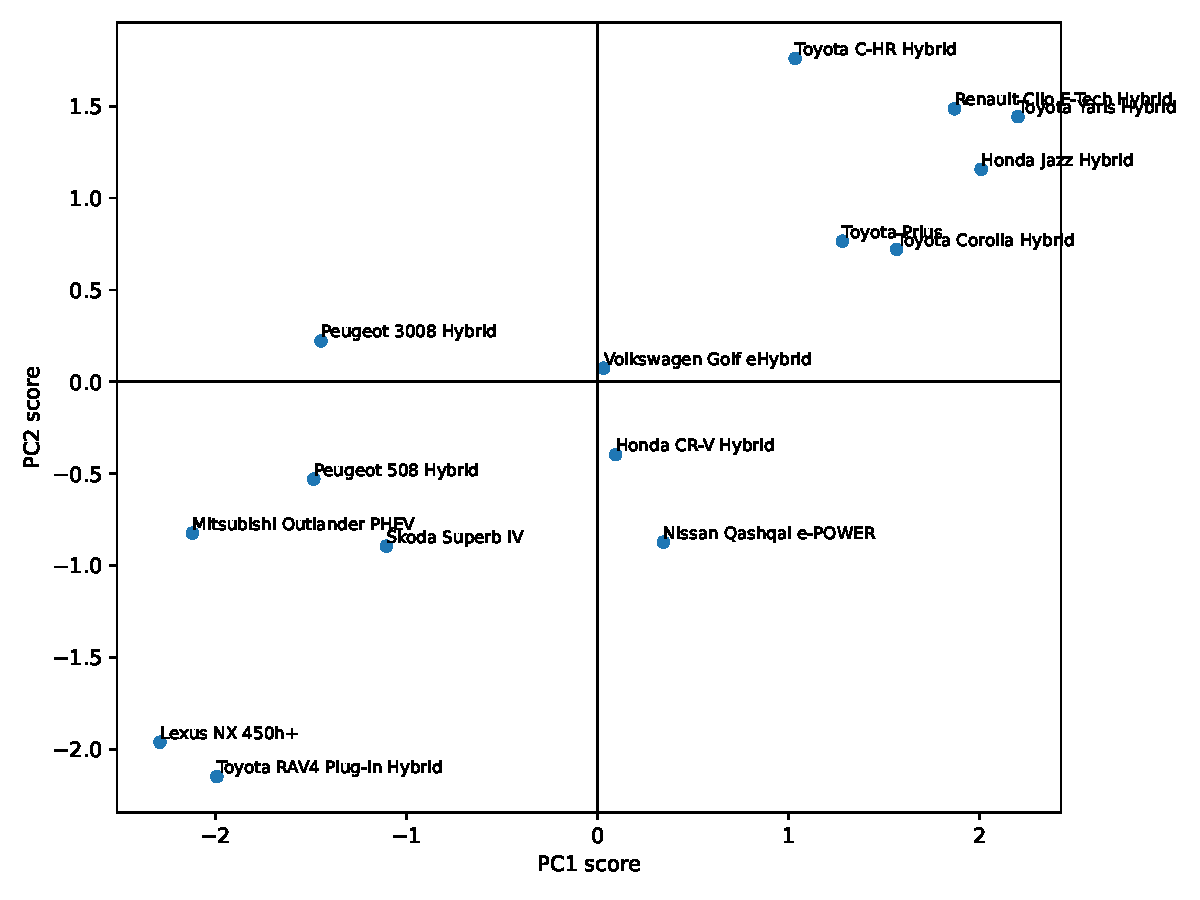
\includegraphics[width=\linewidth]{figs/050-cars-2d-reg.pdf}
    \caption{Dvodimenzionalna projekcija podatkov o avtomobilih, dobljena z regularizacijo L1 ($alpha=3$).}
    \label{fig:cars-2dr}
\end{figure}

Tu morda preseneča lahkota, s katero smo regularizacijo uvedli v metodo analize glavnih komponent. Klasična PCA sicer ima elegantno analitično rešitev\marginnote{PCA, klasično, temelji na lastnem razcepu kovariančne matrike $\Sigma = \tfrac{1}{n}X^\top X$: glavne komponente so lastni vektorji, pripadajoče lastne vrednosti pa podajajo razloženo varianco po posameznih smereh.}, a tak pristop je hkrati precej tog, saj je vezan na točno določeno kriterijsko funkcijo in ortogonalnost komponent. Ko želimo v model vključiti dodatne zahteve, na primer L1- ali L2-regularizacijo, analitična rešitev praviloma ni več na voljo in se moramo vrniti k numerični optimizaciji.

Analizo glavnih komponent lahko razumemo ne le kot zaprto matematično konstrukcijo, temveč tudi kot optimizacijski problem. S tem sicer izgubimo pot do klasične rešitve, a pridobimo tudi precej več svobode: kriterijski funkciji lahko dodajamo člene, ki spodbujajo gladkost, redkost ali druge želene lastnosti komponent. Gradientni sestop zato tu ni le didaktičen približek analitične rešitve, ampak splošnejši okvir, v katerem klasična PCA nastopa le kot njen najpreprostejši primer.

Zgoraj smo uporabili L1 regularizacijo kot primer načina izbora atributov, zmanjšanja kompleksnosti in pomoči pri lažji interpretaciji pomena komponent (uteži). Kako pa je lahko koristna regularizacija L2? Ne pozabimo: podatki, iz katerih gradimo nove, glavne komponente, so lahko šumni
%
\marginnote{Primer takih podatkov so lahko na primer meritve iz molekularne biologije, kjer nam sodobna tehnologija omogoča sočasno izmero več tisoč ali desettisoč spremenljivk (npr. genski izrazi), a bo zaradi cene in manjšega števila vzorcev (npr. merjenih tkiv) podatkov malo, možnost prevelike prilagoditve modela podatkom pa zato ogromna.}
%
. Tudi ta naš, sicer zelo enostaven model, se lahko preveč prilagodi šumu. Regularizacija L2 lahko to prilagoditev ublaži in razvije model, ki je bolj robusten. Za razliko od L1 regularizacije, ki spodbuja redkost in vodi do ničelnih uteži, L2 regularizacija uteži ne izniči, temveč jih enakomerno zmanjša. S tem prepreči, da bi posamezni atributi preveč dominirali pri določanju smeri glavnih komponent. Posledično dobimo bolj stabilne komponente, ki so manj občutljive na majhne spremembe v podatkih.

Intuitivno lahko rečemo, da L2 regularizacija nekoliko ``zgladi'' prostor rešitev: namesto da bi model izbral smer z maksimalno možno varianco, ki je lahko deloma posledica šuma, raje izbere bolj uravnoteženo smer, ki bolje odraža splošno strukturo podatkov. V tem smislu L2 regularizacija uvaja kompromis med maksimalno razloženo varianco in robustnostjo modela.


\section{Točnost, metaparametri učenja}

Zgoraj smo tudi v analizi glavnih komponent uvedli regularizacijo in s tem metaparameter stopnje regularizacije, parameter, katerega vrednost moramo oceniti. A kako? PCA ne napoveduje, kako lahko potem ocenimo kakovost modela in na tej osnovi izberemo primerno stopnjo regularizacije?

O ocenjevanju točnosti in izboru metaparametrov smo pisali že na koncu prejšnjega poglavja. Kvaliteto modela moramo vedno oceniti na ločeni, testni množici. Kvaliteta pri PCA ni vezana na napovedovanje, a smo tudi pri razvoju PCA določili kriterijsko funkcijo — stopnjo razložene variance — ki nam lahko služi za oceno, kako dober je naš model.

Postopek je zato močno podoben, ali bolj rečeno, v osnovni enak kot pri linearni regresiji: podatke razdelimo na učno in testno množico. Na učni množici zgradimo model (določimo glavne komponente), nato pa testne podatke projiciramo na te komponente in na tej projekciji izračunamo razloženo varianco. S tem ocenimo, kako dobro naučene komponente zajamejo strukturo novih podatkov. Pri tem moramo biti pozorni, da vse korake, kot je standardizacija podatkov, izvedemo na učni množici in nato enake transformacije uporabimo na testni množici. V nasprotnem primeru bi lahko nehote uporabili informacijo iz testnih podatkov. Pri tem razloženo varianco na testni množici vedno računamo glede na standardizacijo, naučeno na učni množici, saj bi sicer v oceno nehote vključili informacijo iz testnih podatkov.

Za ocenjevanje primerne vrednosti stopnje regularizacije lahko uporabimo isti trik kot pri linearni regresiji: celotno metodo (standardizacijo, izbor stopnje regularizacije na validacijski množici in gradnjo končnega modela s tako ocenjeno stopnjo regularizacije) zapremo v škatlo, in to v namene neodvisne ocene uspešnosti validiramo na testni množici. Za bolj robustno validacijo lahko tudi tu uporabimo prečno preverjanje. In za končni model celotno škatlo z našo metodo poženemo na vseh podatkih.

\section{Dodatek: glavne komponente so lastni vektorji kovariančne matrike}

V tem razdelku smo se metode PCA lotili z optimizacijo kriterijske funkcije, torej na nekonvencionalen način, tudi zato, ker se bomo s številnimi drugimi tehnikami, kjer nas bo zanimalo modeliranje in razlaga podatkov, spoprijeli prav na ta način. A ima PCA tudi lepo matematično in statistično izpeljavo in podlago in najbrž ne bi bilo prav, če je vsaj ne omenimo. Poteka po naslednjih korakih.

\begin{enumerate} 

\item {\bf Osrediščenje podatkov} Naj bodo \( X \) podatki dimenzij \( n \times d \), kjer je \( n \) število primerov in \( d \) število značilk. Privzamemo, da so podatki osrediščeni, kar pomeni, da za vsako značilko velja:
\[
\frac{1}{n} \sum_{i=1}^{n} X_{i,j} = 0, \quad \text{za vsak } j = 1, 2, \dots, d
\]

\item {\bf Iskanje prve komponente \( \mathbf{u}_1 \)}. Iščemo vektor \( \mathbf{u}_1 \) (dimenzije \( d \times 1 \)), ki določa prvo glavno komponento — smer v prostoru značilk, na katero, če projiciramo podatke, bo varianca projekcij največja. Projekcija podatkovne matrike \( X \) na \( \mathbf{u}_1 \) je:
\[
z = X \mathbf{u}_1
\]
Varianca projekcije \( z \) je:
\[
\mathrm{Var}(z) = \frac{1}{n} \| X \mathbf{u}_1 \|^2 = \frac{1}{n} \mathbf{u}_1^T X^T X \mathbf{u}_1
\]
Ker želimo poiskati smer $\mathbf{u}_1$ z maksimalno varianco, je naša kriterijska funkcija:
\[
\max_{\mathbf{u}_1} \mathbf{u}_1^T S \mathbf{u}_1
\]
kjer malce podrobnejši pogled na zgornjo strukturo pokaže, da je \( S = \frac{1}{n} X^T X \) kovariančna matrika podatkov. Pri tem omejimo dolžino vektorja \( \mathbf{u}_1 \) na 1. To je tudi pogoj, ki mu mora zadostiti kriterijska funkcija:
\[
\mathbf{u}_1^T \mathbf{u}_1 = 1
\]

\item {\bf Optimizacija.} Rešitev problema poiščemo z uporabo Lagrangeovih multiplikatorjev. Postavimo Lagrangeovo funkcijo:
\[
L(\mathbf{u}_1, \lambda) = \mathbf{u}_1^T S \mathbf{u}_1 - \lambda (\mathbf{u}_1^T \mathbf{u}_1 - 1)
\]
in poiščemo stacionarne točke:
\[
\frac{\partial L}{\partial \mathbf{u}_1} = 2 S \mathbf{u}_1 - 2 \lambda \mathbf{u}_1 = 0
\]
\[
S \mathbf{u}_1 = \lambda \mathbf{u}_1
\]
Zgornja enačba je lastna enačba kovariančne matrike. Torej je \( \mathbf{u}_1 \) lastni vektor kovariančne matrike \( S \), pripadajoča lastna vrednost \( \lambda \) pa je:
\[
S \mathbf{u}_1 = \lambda_1 \mathbf{u}_1
\]

\item {\bf Rešitev}. Varianca projekcije je torej podana z:
\[
\mathrm{Var}(z) = \frac{1}{n} \| X \mathbf{u}_1 \|^2 = \mathbf{u}_1^T S \mathbf{u}_1
\]
Ker pa iz lastne enačbe velja:
\[
S \mathbf{u}_1 = \lambda_1 \mathbf{u}_1
\]
sledi:
\[
\mathbf{u}_1^T S \mathbf{u}_1 = \mathbf{u}_1^T \lambda_1 \mathbf{u}_1 = \lambda_1 (\mathbf{u}_1^T \mathbf{u}_1) = \lambda_1
\]
ker smo predpostavili, da je \( \mathbf{u}_1^T \mathbf{u}_1 = 1 \). Zato velja:
\[
\mathrm{Var}(z) = \lambda_1
\]
kar pomeni, da je lastna vrednost \( \lambda_1 \) enaka varianci podatkov v smeri prve glavne komponente \( \mathbf{u}_1 \).

Ker želimo maksimizirati varianco projekcije, med vsemi možnimi lastnimi vektorji kovariančne matrike za prvo komponento vzamemo tisti lastni vektor, ki ustreza največji lastni vrednosti \( \lambda_1 \). Varianca v smeri \( \mathbf{u}_1 \) je enaka tej lastni vrednosti:
%
\[
\mathrm{Var}(z) = \lambda_1
\]
Vse ostale komponente so torej lastni vektorji, urejeni po padajočih lastnih vrednostih, ki podajajo razloženo varianco po posameznih komponentah.
\end{enumerate}

Zgornja izpeljava je elegantna in vzpostavi povezavo med glavnimi komponentami in prostorom lastnih vektorjev kovariančne matrike. Tu tudi postane jasno, zakaj so glavne komponente povezane s korelacijami med atributi. A kljub eleganci rešitve ta ne omogoča razširitev tehnike z regularizacijo, kjer je pristop, ki uporablja gradientni sestop, kot smo ga razvili v poglavju, prava rešitev.
\chapter{Dvodimenzionalne vložitve podatkov}

V tem poglavju obravnavamo metode, ki primere vložijo v dvodimenzionalni prostor, tako da geometrijski odnosi med točkami čim bolje odražajo odnose med primeri v izvirnem prostoru. Takšne vložitve uporabljamo predvsem za prikaz strukture podatkov v namene odkrivanja zanimivih vzorcev in skupin, pa tudi v namene rangiranja in odkrivanja odnosov med posameznimi primeri iz učne množice.

Analiza glavnih komponent, o kateri smo govorili v prejšnjem poglavju, ni vložitev v istem smislu kot metode, obravnavane v tem poglavju. Metoda glavnih komponent je projekcijska metoda, ki oblikuje matematični predpis, recimo \( U \) (matrika, sestavljena iz smernih vektorjev glavnih komponent \( u_1 \) in \( u_2 \)), ki podatke \( X \) projicira v dve dimenziji, torej \( Z = XU \). Projekcija v splošnem ni isto kot vložitev. Pri PCA iščemo preslikavo \( f(x) \), ki podatke projicira v nov koordinatni sistem, pri metodah, obravnavanih v tem poglavju, pa iščemo neposredno postavitev točk \( y_1, \dots, y_n \in \mathbb{R}^2 \),
%
\marginnote{Oznaka $y_i$ tu ne predstavlja razreda (kot pri napovednih modelih), temveč koordinate točke v vložitvi primera $x_i$ oziroma položaj tega primera v dvodimenzionalnem prostoru.}
%
ki čim bolje ohranja izbrane odnose med primeri. Zato takšne metode praviloma ne podajo enostavne preslikave za nove podatke v isti prostor.

Ogledali si bomo tri pristope k dvodimenzionalnim vložitvam podatkov: večrazsežno lestvičenje (MDS), metodo t-SNE in vložitve s silami. Prva je pomembna z zgodovinskega vidika, druga poudarja lokalno strukturo podatkov, tretja pa izhaja iz vizualizacije omrežij. Pri majhnih podatkovnih množicah so lahko vložitve MDS, t-SNE in metod s silami podobne, pri večjih in visokorazsežnih podatkih pa pridejo razlike med pristopi precej bolj do izraza.

Skupen vsem trem opisanim metodam je osnovni pristop vložitve primerov v dve dimenziji. Uporabili bomo kriterijsko funkcijo, ki izhaja iz razdalj med primeri v izvornem prostoru in jih na ustrezen način poveže s položaji točk v vložitvenem prostoru. Začetno vložitev dobimo tako, da točke (primere) v ravnini razporedimo naključno, nato pa njihove položaje postopoma popravljamo v smeri gradienta kriterijske funkcije glede na koordinate teh točk. Tokrat torej model ne predstavljajo uteži ali parametri preslikave, temveč kar same koordinate točk v vložitvi, zato je število parametrov enako $2n$, kjer je $n$ število primerov.

\section{Podatki}


Začnimo kar s podatki.
%
\marginnote{Podatke lahko v tem poglavju opišemo zgolj z razdaljami med primeri, brez eksplicitnega atributnega zapisa. Tak opis pa ni neposreden vhod za PCA, saj ta metoda potrebuje predstavitev primerov z atributi.}
%

Vse metode, ki jih bomo v tem poglavju predstavili, lahko izhajajo iz razdalj ali podobnosti med primeri. Predpostavili bomo, da so ti odnosi že podani. Tokrat primerov torej ne bomo opisovali eksplicitno z atributi, kot smo bili vajeni v prejšnjih poglavjih, temveč zgolj z razdaljami med njimi. Te razdalje bi običajno zapisali v (simetrični) matriki, lahko pa jih predstavimo tudi s spodnjim slovarjem:

\vspace*{3mm}
\begin{lstlisting}
distances = {
    ("Novo Mesto", "Maribor"): 170,
    ("Novo Mesto", "Celje"): 83,
    ("Novo Mesto", "Koper"): 169,
    ("Novo Mesto", "Kranj"): 99,
    ("Novo Mesto", "Ljubljana"): 72,
    ("Novo Mesto", "Postojna"): 116,

    ("Maribor", "Celje"): 55,
    ("Maribor", "Koper"): 232,
    ("Maribor", "Kranj"): 156,
    ("Maribor", "Ljubljana"): 128,
    ("Maribor", "Postojna"): 178,

    ("Celje", "Koper"): 183,
    ("Celje", "Kranj"): 105,
    ("Celje", "Ljubljana"): 77,
    ("Celje", "Postojna"): 130,

    ("Koper", "Kranj"): 128,
    ("Koper", "Ljubljana"): 107,
    ("Koper", "Postojna"): 58,

    ("Kranj", "Ljubljana"): 30,
    ("Kranj", "Postojna"): 77,

    ("Ljubljana", "Postojna"): 53,
}
\end{lstlisting}

\section{Večrazsežno lestvičenje}

Zapišimo 
%
\marginnote{Večrazsežno lestvičenje (angl.~\emph{multidimensional scaling}, MDS) so razvili Torgerson (1952), Shepard (1962) in Kruskal (1964) v okviru psihometrije, področja, ki se ukvarja z merjenjem psiholoških lastnosti (npr. zaznav, podobnosti med dražljaji in preferenc) z uporabo statističnih metod.}
%
razdaljo med primeroma \( i \) in \( j \) z \( d_{ij} \). V večrazsežnem lestvičenju želimo primere urediti v dvodimenzionalnem prostoru tako, da vsak primer \( i \) opišemo s koordinatama \( y_i = (y_{i1}, y_{i2}) \in \mathbb{R}^2 \). V tem ciljnem prostoru naj bo razdalja med primeroma evklidska,
\[
\|y_i - y_j\| = \sqrt{(y_{i1} - y_{j1})^2 + (y_{i2} - y_{j2})^2},
\]
torej takšna, kot bi jo dobili pri običajnem razsevnem diagramu.

Cilj večrazsežnega lestvičenja 
%
\marginnote{Izraz \emph{lestvičenje} (angl. \emph{scaling}) pomeni razporejanje objektov na lestvico tako, da razdalje med njimi odražajo njihove medsebojne razlike ali podobnosti. Pridevnik \emph{večrazsežno} (angl.~\emph{multidimensional}) poudarja, da te lestvice ne tvorimo le v eni dimenziji, temveč v večrazsežnem prostoru, najpogosteje v dveh ali treh dimenzijah.}
%
je čim bolje ohraniti dane razdalje, torej naj bodo razdalje \( \|y_i - y_j\| \) v vložitvenem prostoru čim bližje izhodiščnim razdaljam \( d_{ij} \). Skladno s tem večrazsežno lestvičenje minimizira kriterijsko funkcijo
\[
J(Y) = \sum_{i < j} \bigl( \|y_i - y_j\| - d_{ij} \bigr)^2,
\]
kjer \( Y = \{y_1, \dots, y_n\} \) predstavlja iskano postavitev točk v ravnini.

Evklidska razdalja v vložitvenem prostoru je torej v celoti odvisna od položajev točk, ki predstavljajo primere; ti položaji pa so tudi parametri našega modela. Te bomo iskali z gradientnim sestopom, pri čemer bomo uporabili strojno odvajanje. Knjižnico za strojno odvajanje in učenje z gradientnim sestopom smo že zgradili v prejšnjih poglavjih, zato tu podajamo le kodo razreda za predstavitev modela večrazsežnega lestvičenja.

\vspace*{3mm}
\begin{lstlisting}
class MDS:
    def __init__(self, items):
        random.seed(100)
        self.pos = {i: [Value(random.uniform(-1, 1)) for _ in range(2)]
                    for i in sorted(items)}
    
    def parameters(self):
        return [p for pos in self.pos.values() for p in pos]
    
    def d(self, a, b):
        return sum([(ai - bi) ** 2 for ai, bi in \
                    zip(self.pos[a], self.pos[b])]) ** 0.5

    def loss(self, xs, ys):
        n = len(xs)
        return sum((self.d(*pair) - y) ** 2 \
                   for pair, y in zip(xs, ys)) / Value(n)
\end{lstlisting}

Razred \texttt{MDS} zgradi računski graf kriterijske funkcije za večrazsežno lestvičenje za dane vhodne podatke (razdalje). Vsakemu primeru priredimo naključno začetno pozicijo v ravnini (\texttt{self.pos}), te koordinate pa predstavljajo parametre modela. Metoda \texttt{d} izračuna evklidsko razdaljo med dvema primeroma v trenutni vložitvi, \texttt{loss} pa meri odstopanje med temi razdaljami in podanimi razdaljami \( d_{ij} \). 

Z gradientnim sestopom nato popravljamo položaje točk tako, da se ta napaka čim bolj zmanjša:

\vspace*{3mm}
\begin{lstlisting}
items = sorted(list(set(i for pair in distances.keys() for i in pair)))
pairs = list(distances.keys())
targets = [distances[p] for p in pairs]

model = MDS(items)
model = train(model, pairs, targets, n_epochs=1000, 
              learning_rate=0.1, report_every=100)
\end{lstlisting}

Mest je v naši učni množici malo, optimizacija pa konvergira hitro. Namesto izpisa pozicij posameznih mest je tu seveda bolj na mestu izris podatkovne karte:

\vspace*{3mm}
\begin{lstlisting}
plt.figure(figsize=(4, 4))
for city in sorted(items):
    x, y = model(city)
    plt.scatter(x.data, y.data, color="k", s=10)
    plt.annotate(
        city,
        (x.data, y.data),
        xytext=(0, 4),
        textcoords="offset points",
        ha="center",
        va="bottom",
    )
plt.savefig("mds-cities.pdf")
\end{lstlisting}

Karto mest prikazuje slika~\ref{fig:mds}.
%
\marginnote{Našo karto slovenskih mest bi lahko za lažjo primerjavo s geografskimi kartami, na katere smo navajeni, zasukali za 180 stopinj.}
%
Malce je zasukana in narobe obrnjena, a kdo pravi, da mora biti sever na vrhu in da gledamo od zgoraj. Relacije med mesti so sicer kar prave. Maribor, Celje, Ljubljana, Postojna in Koper so na glavni diagonali v pravem vrstnem redu, Kranj malce stran, Novo mesto na drugi strani. Vhodni podatki so vsebovali cestne razdalje med mesti, ki niso enake zračnim; evklidska razdalja v prostoru vložitve pa ustreza zračni. Najbrž je to glavni izvor za kakšne manjše napake, a v splošnem nam je rekonstrukcija pozicije slovenskih mest iz cestnih razdalj dobro uspela.

\begin{marginfigure}
    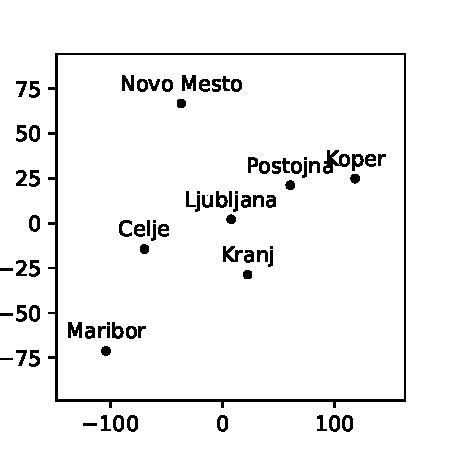
\includegraphics[width=\linewidth]{figs/060-mds-cities.pdf}
    \caption{Dvodimenzionalna vložitev z večrazsežnim lestvičenjem.}
    \label{fig:mds}
\end{marginfigure}

Opozorilo sicer: MDS-vložitev z enako dobro vrednostjo kriterijske funkcije $J(Y)$ je nešteto. Pri nespremenjeni vrednosti kriterijske funkcije vložitve lahko poljubno rotiramo in zrcalimo. Vse te transformacije ohranjajo razdalje in pravzaprav samo te nastopajo v kriterijski funkciji. Dobljene osi zato nimajo pomena in jih kot takih ne moremo povezati s kakšno razlago. Drugače kot pri PCA torej. A spomnimo: pri PCA izhajamo iz atributno predstavljenih primerov, tu pa, pri MDS, iz razdalj.

\begin{exercise}{Ista struktura, drugačen zemljevid.}
Isto podatkovno množico večkrat vloži z različnimi naključnimi začetnimi položaji ter primerjaj končne vložitve, njihove vrednosti izgube in medsebojne razdalje, da ugotoviš, koliko je rezultat odvisen od inicializacije.
\end{exercise}

\begin{exercise}{Koliko razdalj potrebujemo za zemljevid?}
Vzemi podatke o slovenskih mestih iz poglavja. Najprej uporabi vse podane razdalje in z MDS rekonstruiraj zemljevid. Nato naključno odstranjuj vedno več razdalj (npr.\ 10\%, 25\%, 50\%, 75\%) in opazuj, kako se spreminja kakovost vložitve. Kdaj postane problem premalo določen? Ali obstajajo razdalje, katerih odstranitev bistveno bolj škodi kot odstranitev drugih? Kakovost vložitve lahko opazuješ izkustveno, s karto, lahko pa uporabiš tudi isto metriko kot pri ocenjevanju izgube pri MDS, le da to oceno izračunaš iz celotne množice podatkov (torej ne samo iz te, iz katerih iz vzorčil učno množico).
\end{exercise}

\begin{exercise}{Odpornost vložitev na šum.}
    Na podatkih o cestnimi razdaljami slovenskih mest izberi eno od razdalj ter njej umetno dodaj veliko napako (npr.\ razdaljo Ljubljana--Koper povečaj za 100~km). Nato ponovno izračunaj MDS-vložitev in primerjaj položaje mest pred in po spremembi. Poskus ponovi za več velikosti napake in kasneje na več različnih parov mest. Kako se na napake odziva večrazredno lestvičenje? Katere napačne meritve najbolj pokvarijo vložitev?
\end{exercise}
    

\section{Vložitve sosedov}

Večrazsežno lestvičenje ima skriti problem: kriterijska funkcija kvadrira razliko razdalj iz vhodnih podatkov in vložitvenega prostora. Učenje modela z gradientnim sestopom se bo zato bolj ``potrudilo'' pri zmanjševanju večjih odstopanj. Če odstopanja merimo v deležih, na primer v odstotkih, in če na primer na vložitvi razdalje odstopajo od vhodnih za $10\%$, bo odstopanje med Ljubljano in Kranjem imelo dosti manjši vpliv na učenje kot odstopanje med Koprom in Mariborom. MDS torej teži k ohranjanju predvsem tistih večjih razdalj. Vpliv krajših razdalj med sosednjimi primeri je veliko manjši.

Ohranjanje večjih razdalj je seveda zaželeno, če želimo pridobiti podatkovne karte s primernimi globalnimi ureditvami. A mnogokrat nas pri podatkovni analitiki zanimajo predvsem soseščine in na podatkovnih kartah morda iščemo samo skupine podatkov ter jih skušamo interpretirati, pri čemer nas globalni odnosi oziroma skupine, ki so oddaljene druga od druge, ne zanimajo. Tako bi nas zanimale vizualizacije, kjer so izražene skupine primerov, ki so si med sabo podobni, in nas sama interpretacija razdalje med skupinami, ki so si med seboj oddaljene, ne zanima. Taka vizualizacija je na primer prikazana na sliki~\ref{fig:mds-tsne} na desni strani in je očitno zelo različna od vizualizacije istih podatkov, kot jo pridela MDS.

\begin{figure}
    \centering
    \fbox{%
        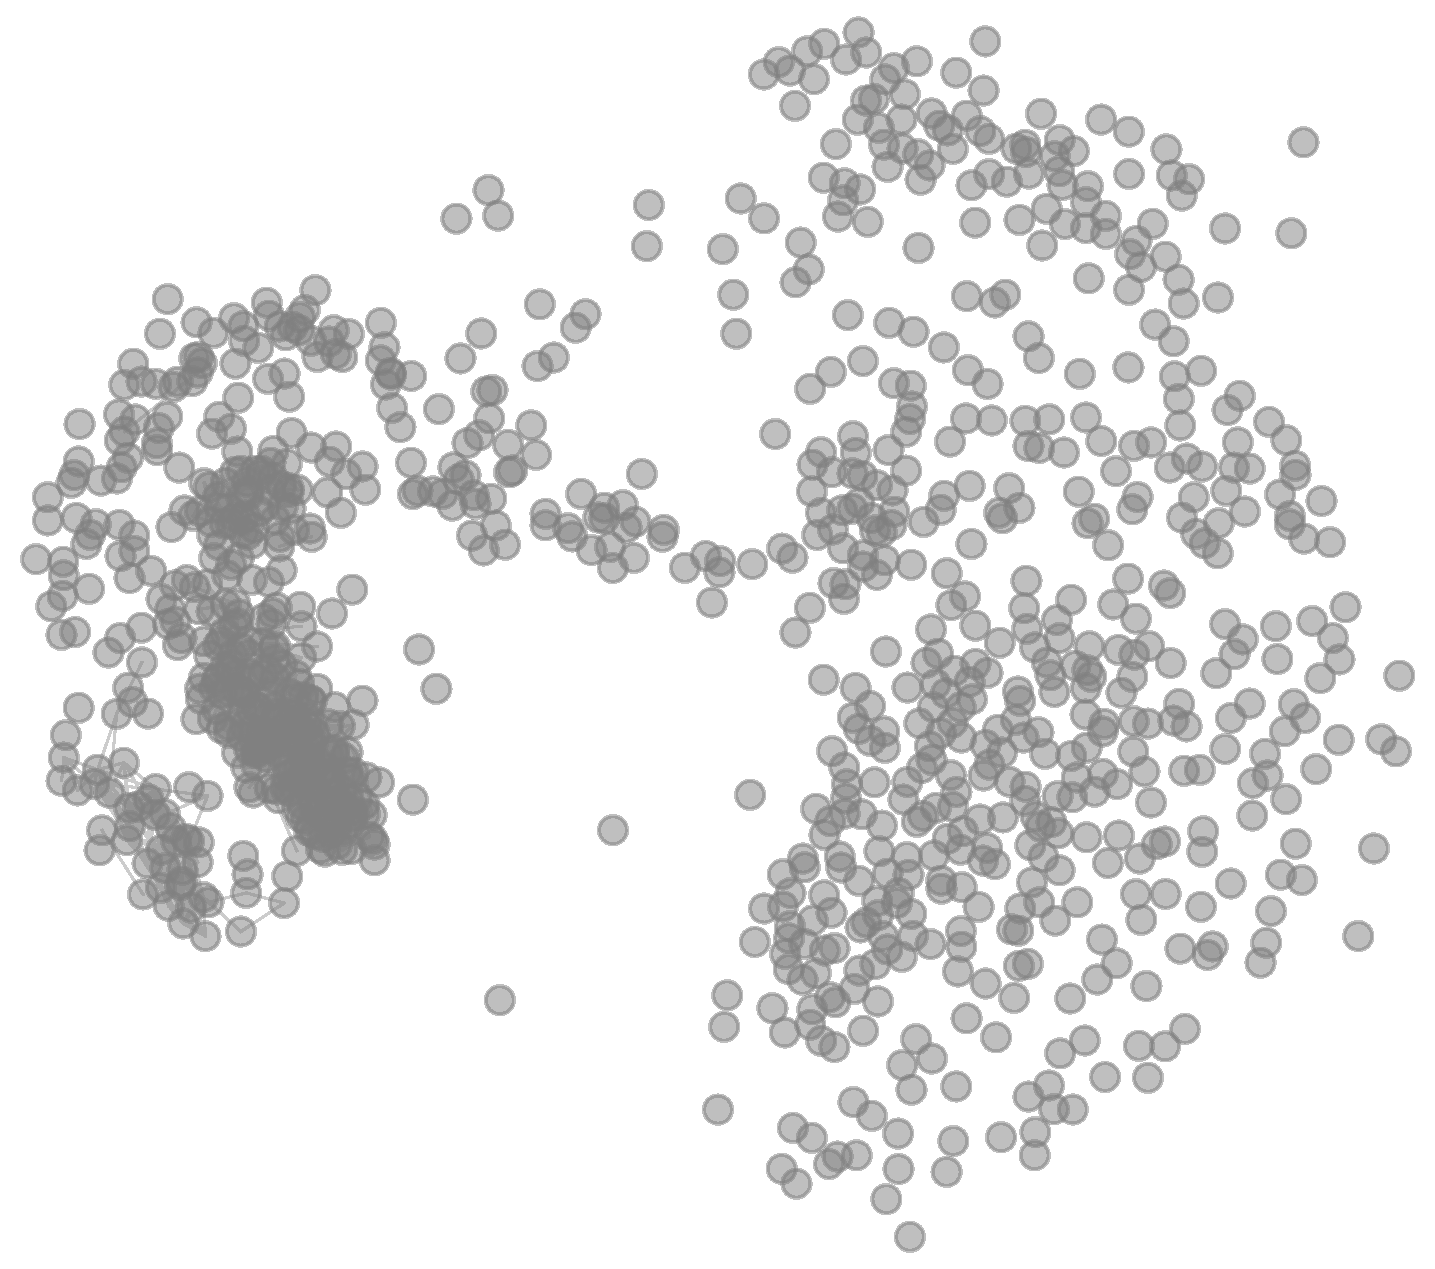
\includegraphics[width=0.45\textwidth]{figs/060-mds-bone-marrow.pdf}
    }
    \hfill
    \fbox{%
        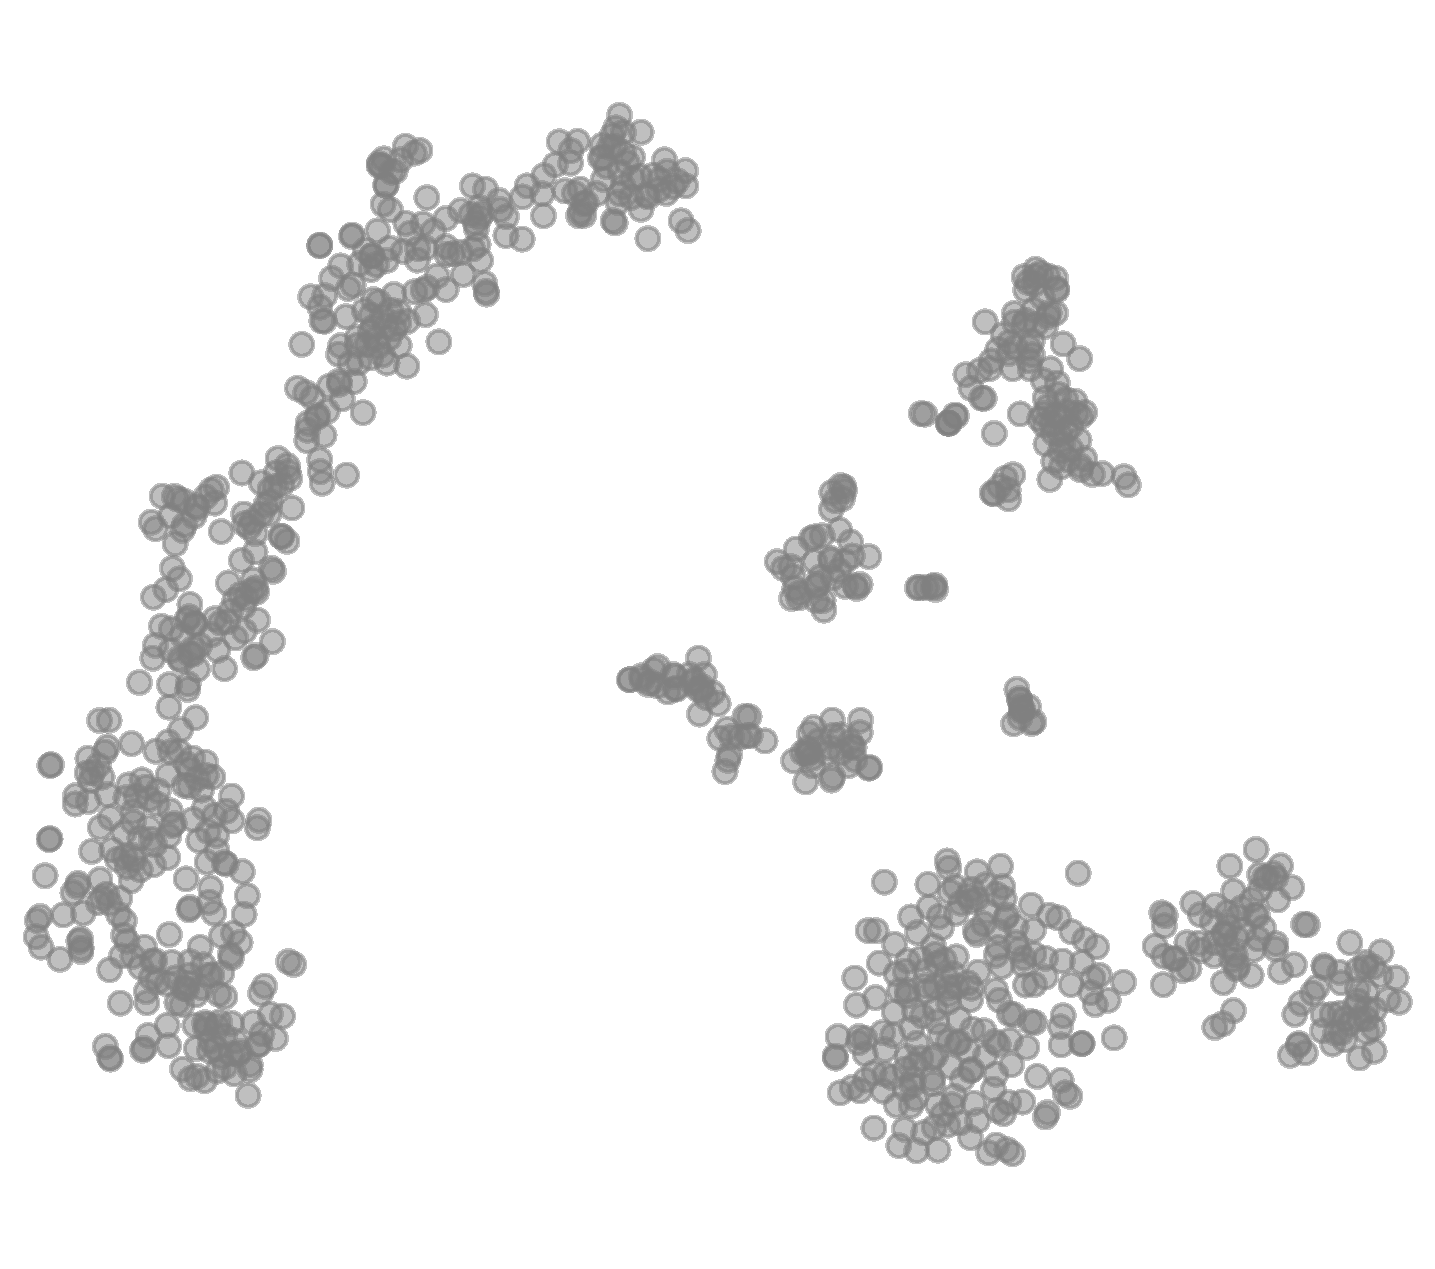
\includegraphics[width=0.45\textwidth]{figs/060-t-sne-bone-marrow.pdf}
    }
    \caption{Primerjava vložitev MDS (levo) in t-SNE (desno) na podatkih o izražanju genov v celicah kostnega mozga (vzorec tisoč celic in izrazi tisoč genov). Skupine točk naj bi pripadale posameznim celičnim tipom.}
    \label{fig:mds-tsne}
\end{figure}

Zanima nas torej ohranjanje soseščine. Za to potrebujemo mero, ki pove, kako blizu so si primeri v izvornem prostoru, in mero, ki pove, kako blizu so si v prostoru vložitev. Ti meri morata zanemariti primere, ki so si daleč, in se osredotočiti le na bližnje primere. Tu lahko uporabimo trik: namesto razdalje bomo ocenili verjetnost, da sta si dva primera blizu, v izvornem prostoru in prostoru vložitev, kot kriterijsko funkcijo pa ocenili podobnost med tema vektorjema verjetnosti, kjer z vektorjema mislimo seznama verjetnosti bližine vseh parov primerov.

Lotimo se tega bolj formalno. Kot pri MDS naj bo $x_i$ primer v izvornem prostoru in $y_i$ njegova predstavitev v vložitvi. Za vsak par primerov $(i,j)$ določimo podobnost v izvornem prostoru kot pogojno verjetnost
\[
p_{j|i} = \frac{\exp\!\left(-\frac{\|x_i - x_j\|^2}{2\sigma_i^2}\right)}{\sum_{k \ne i} \exp\!\left(-\frac{\|x_i - x_k\|^2}{2\sigma_i^2}\right)}.
\]
Ta verjetnost pove, kako verjetno bi izbrali primer $j$ kot soseda primera $i$. Pri tem parameter $\sigma_i$ določa ``širino'' okolice okoli $x_i$. Ker pogojne verjetnosti \( p_{j \mid i} \) na splošno niso simetrične, torej praviloma ne velja \( p_{j \mid i} = p_{i \mid j} \), ju pri t-SNE združimo v simetrično skupno verjetnost
\[
p_{ij} = \frac{p_{j \mid i} + p_{i \mid j}}{2n},
\]
kjer je \( n \) število vseh primerov.

V prostoru vložitev podobno določimo verjetnosti bližine, vendar uporabimo porazdelitev z debelejšimi repi (Studentovo $t$-porazdelitev z eno stopnjo prostosti):
\[
q_{ij} = \frac{\left(1 + \|y_i - y_j\|^2\right)^{-1}}{\sum_{k \ne l} \left(1 + \|y_k - y_l\|^2\right)^{-1}}.
\]
Ta izbira zmanjša problem zgoščanja, saj omogoča izrazitejšo predstavitev večjih razdalj v vložitvi kot pri Gaussovi porazdelitvi.

Cilj tega pristopa je poiskati takšne vložitve $y_i$, da so porazdelitve $p_{ij}$ in $q_{ij}$ čim bolj podobne. To dosežemo z minimizacijo Kullback-Leiblerjeve divergence:
\[
\mathcal{L}(Y) = \sum_{i \ne j} p_{ij} \log \frac{p_{ij}}{q_{ij}}.
\]
Ta kriterijska funkcija kaznuje predvsem primere, kjer sta si točki v izvornem prostoru blizu (velik $p_{ij}$), v vložitvi pa daleč narazen (majhen $q_{ij}$), zato spodbuja ohranjanje lokalne strukture podatkov.

Kriterijsko funkcijo,
%
\marginnote{Metodo SNE sta predlagala Geoffrey E. Hinton in Sam T. Roweis (2002), t-SNE pa Hinton in Laurens van der Maaten (2008). Hinton je tudi eden od očetov sodobne umetne inteligence in je leta 2024 za svoje raziskovalno delo prejel Nobelovo nagrado.}
%
kot je določena zgoraj, uporablja metoda t-SNE (angl.~\emph{t-distributed Stochastic Neighbor Embedding}). Ta pristop je nadgradil starejšo metodo SNE, ki je prav tako temeljila na primerjavi verjetnostnih porazdelitev bližin med pari primerov v izvornem prostoru in prostoru vložitev. A je imel SNE nekaj pomembnih pomanjkljivosti. Prvič, uporabljal je nesimetrične verjetnosti $p_{j|i}$ in $q_{j|i}$, kar je otežilo optimizacijo in interpretacijo. Drugič, zaradi uporabe Gaussove porazdelitve tudi v prostoru vložitev je trpel za t.~i.\ problemom ``zgoščanja'' (angl.~\emph{crowding problem}), kjer se večje razdalje težko ustrezno predstavijo v nizkodimenzionalnem prostoru, zato se točke pogosto preveč nagnetejo skupaj.

Metoda t-SNE odpravi glavni pomanjkljivosti metode SNE na dva načina: uporabi simetrično podobnost \( p_{ij} \) in v prostoru vložitve uvede Studentovo \( t \)-porazdelitev.

V nadaljevanju ne bomo implementirali celotne standardne različice metode t-SNE, temveč poenostavljeno različico, ki ohrani osnovno idejo: bližnji pari v izvornem prostoru naj imajo visoko verjetnost tudi v prostoru vložitve, kriterijska funkcija pa naj meri razliko med obema porazdelitvama. 

\vspace*{3mm}
\begin{lstlisting}
class tSNE:
    def __init__(self, items, sigma=40.0, eps=1e-12):
        random.seed(100)
        self.pos = {
            i: [Value(random.uniform(-1, 1)) for _ in range(2)]
            for i in sorted(items)
        }
        self.sigma = sigma  # constant bandwidth of the Gaussian
        self.eps = eps  # parameter for numerical stability

    def parameters(self):
        return [p for pos in self.pos.values() for p in pos]

    def p_distribution(self, pairs, distances):
        unnorm = []
        for d in distances:
            pij = math.exp(-(d ** 2) / (2 * self.sigma ** 2))
            unnorm.append(pij)

        z = sum(unnorm) + self.eps
        return [p / z for p in unnorm]

    def sqdist(self, a, b):
        return sum((ai - bi) ** 2 \
                   for ai, bi in zip(self.pos[a], self.pos[b]))

    def q_distribution(self, pairs):
        numerators = []
        for a, b in pairs:
            numerators.append((Value(1.0) + self.sqdist(a, b)) ** -1)

        z = sum(numerators)
        return [q / z for q in numerators]

    def loss(self, pairs, distances):
        p = self.p_distribution(pairs, distances)
        q = self.q_distribution(pairs)

        loss = Value(0.0)
        for pij, qij in zip(p, q):
            loss = loss + Value(pij) * \
              (math.log(pij + self.eps) - (qij + self.eps).log())

        return loss
\end{lstlisting}

Razred `tSNE` v konstruktorju `\_\_init\_\_` najprej za vsak primer naključno inicializira dvodimenzionalno vložitev `self.pos`. Metoda `p\_distribution` iz podanih razdalj v izvornem prostoru izračuna porazdelitev podobnosti $p_{ij}$ tako, da vsako razdaljo pretvori v utež z Gaussovo funkcijo in nato vse uteži normalizira v verjetnosti. Za prostor vložitev metoda `sqdist` izračuna kvadrat evklidske razdalje, `q\_distribution` pa to uporabi tako da iz trenutnih položajev točk izračuna porazdelitev $q_{ij}$. Pri tem uporabi jedro oblike
\[
(1 + \|y_i - y_j\|^2)^{-1}.
\]
Kriterijsko funkcijo smo implementirali v metodi `loss`, ki najprej določi porazdelitvi `p` in `q`, potem pa za izračun Kullback-Leiblerjeve divergence za vse pare sešteje $p_{ij}\log(p_{ij}/q_{ij})$.

Tu uporabljamo poenostavljeno različico metode t-SNE. V standardni izvedbi se širina Gaussovega jedra ne določi z enim samim parametrom, temveč se za vsako točko posebej prilagodi tako, da ustreza izbrani perpleksnosti (angl.~\emph{perplexity}). Pogosto se uporablja tudi zgodnje pretiravanje (angl.~\emph{early exaggeration}), pri katerem v začetnih iteracijah povečamo vrednosti $p_{ij}$ in s tem poudarimo oblikovanje lokalnih skupin.

\marginnote{V naši poenostavljeni implementaciji parameter $\sigma$ nadomesti perpleksnost standardnega t-SNE. Ta poskus eksperimentalno pokaže njegovo vlogo: z njim uravnavamo, koliko lokalne ali globalne strukture vložitev ohranja.}
\begin{exercise}{Kakšna je vloga parametra $\sigma$?}
Na podatkih z več jasno ločenimi skupinami izvedi t-SNE za različne vrednosti $\sigma$. Opazuj, kako se spreminja oblika vložitve. Pri majhnih vrednostih bo metoda poudarjala zelo lokalne sosede, pri velikih pa se bo približevala globalni strukturi. Poskusi najti vrednost, pri kateri so skupine najbolj jasno ločene.
\end{exercise}

\begin{exercise}{t-SNE z razredno informacijo.}
Izberi podatkovno množico za klasifikacijo in kriterijski funkciji t-SNE dodaj člen, ki spodbuja, da so primeri istega razreda v vložitvi bližje skupaj, primeri različnih razredov pa bolj narazen; nato postopoma povečuj utež tega člena in opazuj, kako se spreminjata geometrija vložitve ter ločenost razredov.
\end{exercise}

Uporaba zgornje implementacije od tu dalje ni prav nič drugačna kot za MDS:
\vspace*{3mm}
\begin{lstlisting}
model = tSNE(items, sigma=40.0)
model = train(model, pairs, targets, 
              n_epochs=3000, learning_rate=0.05, report_every=100)
\end{lstlisting}
Tudi tu so na vhodu razdalje, na izhodu pa vložitve primerov. Te znova lahko prikažemo na razsevnem diagramu (slika~\ref{fig:tsne}). Dobljena vložitev ni bistveno drugačna od tiste pri MDS. Kar je sicer zanimivo, saj gre za metodi, ki imata popolnoma drugačno kriterijsko funkcijo. Razlike med MDS in t-SNE se zares pokažejo pri večjih in visokorazsežnih podatkih. Tam je lokalna soseščina pogosto informativnejša od globalne geometrije, zato t-SNE bolje izpostavi skupine podobnih primerov, medtem ko MDS še naprej sledi predvsem globalnim razdaljam. Primer take, zelo različne vložitve kaže slika~\ref{fig:mds-tsne}, kjer je pri MDS težko med sabo ločiti skupine, ki so jasno razvidne v prikazu vložitev t-SNE.

\marginnote{Pri majhnih množicah, kot so mesta v tem poglavju, sta vložitvi MDS in t-SNE pogosto skoraj enaki, zato razlika med globalno in lokalno strukturo ostane abstraktna. Poskus na visokorazsežnih podatkih to ilustrira neposredno: ko skupine v izvornem prostoru približujemo, MDS zlije vložitev, t-SNE pa naj bi ohranjal ločene gruče.}
\begin{exercise}{Kaj vidi posamezna metoda?}
Na majhnih množicah sta MDS in t-SNE pogosto podobni; zato ustvari tri dobro ločene skupine točk v desetdimenzionalnem prostoru, izračunaj vse medsebojne razdalje in jih vloži z MDS ter t-SNE. Nato postopoma zmanjšuj razdaljo med skupinami. Primerjaj, pri kateri stopnji prekrivanja posamezna metoda še uspe ločiti skupine. Kaj ohranja MDS in kaj ohranja t-SNE?
\end{exercise}

\begin{exercise}{Ali lahko zaupamo razdaljam na sliki?}
Za izbrane pare točk primerjaj njihove razdalje v izvirnem visokorazsežnem prostoru z razdaljami v dvodimenzionalni vložitvi ter poišči primere, kjer bližina ali oddaljenost na sliki daje posebej zavajajoč vtis. Kako bi na vizualizaciji izpostavil ``napačne'' razdalje? Kako bi zgradil uporabniški vmesnik za iskanje teh?
\end{exercise}

\begin{marginfigure}
    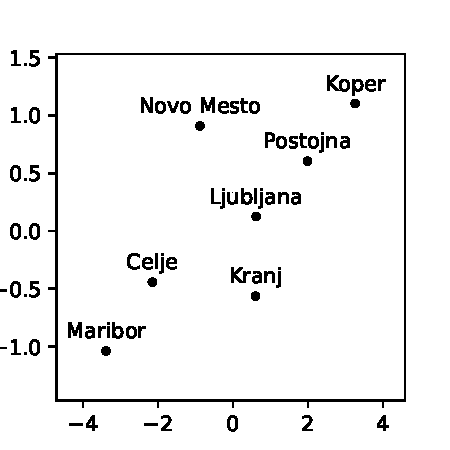
\includegraphics[width=\linewidth]{figs/060-tsne-mesta.pdf}
    \caption{Dvodimenzionalna vložitev s t-SNE.}
    \label{fig:tsne}
\end{marginfigure}

\section{Vložitve s silami}

Oglejmo si še tretji pristop. Obravnavamo ga zato, ker se po izhodišču precej razlikuje od prejšnjih dveh in ker je zelo uveljavljen na področju vizualizacije omrežij. Pristop predpostavi, da so primeri točke, med katerimi delujejo sile. Pari primerov, za katere poznamo razdalje,
%
Tu uvedemo še pomembno razliko glede na prejšnje primere: doslej smo obravnavali podatke, pri katerih so bile razdalje podane za vse pare primerov, kar pa za metode s silami ni nujno. Pogosto namreč zadošča, da poznamo razdalje ali povezave le za izbrane pare.
%
povežemo z ``vzmetmi'', ki skušajo ohranjati predpisano dolžino, hkrati pa med vsemi pari deluje še odbojna sila, ki preprečuje, da bi se točke preveč zgostile. Položaj točk v ravnini nato dobimo z iskanjem ravnovesja sil, ki ga poiščemo z minimizacijo ustrezne energijske funkcije. Čeprav je tak pristop bil razvit na področju vizualizacije omrežij, kjer želimo pregledno razporediti vozlišča grafa, ga enako uspešno uporabimo tudi za vložitve podatkov.

Kot prej, naj bo $y_i \in \mathbb{R}^2$ znova položaj primera $i$ v ravnini. Za pare primerov $(i,j)$, za katere poznamo razdaljo $d_{ij}$, uvedemo ``vzmetno'' energijo
\[
E_{\text{vzmeti}} = \frac{1}{|E|} \sum_{(i,j)\in E} \bigl( \|y_i - y_j\| - d_{ij} \bigr)^2,
\]
kjer $E$ označuje množico parov z znanimi razdaljami. Ta člen sili povezane pare, da v vložitvi ohranjajo predpisane razdalje.

Med vsemi pari primerov hkrati deluje še odbojna sila, ki jo opišemo z energijo
\[
E_{\text{odboj}} = \frac{1}{\binom{n}{2}} \sum_{i<j} \frac{1}{\|y_i - y_j\|},
\]

Skupno energijo zapišemo kot vsoto obeh členov
\[
E = E_{\text{vzmeti}} + C \, E_{\text{odboj}},
\]
kjer konstanta \(C\) določa relativni vpliv odbojnega člena. Rešitev so takšni položaji točk $y_i$, ki to skupno energijo minimizirajo.

Zgornja kriterijska funkcija je na prvi pogled še najbolj podobna tej, ki jo uporablja MDS. A podobnost je zgolj navidezna in velja le, ko so razdalje podane za vse pare. Pri MDS en sam člen enakovredno obravnava vse pare primerov in skuša globalno ohraniti vse razdalje. Pri silno vodenih vložitvah pa se kriterijska funkcija razcepi na več delov: vzmeti delujejo le med izbranimi pari (npr.\ povezanimi v omrežju) in skrbijo za lokalno strukturo, odboj pa deluje med vsemi pari in preprečuje zgoščanje točk. S tem dobimo ravnovesje med lokalnim ohranjanjem razdalj in globalnim razmikom točk, kar vodi do bistveno drugačnih vložitev kot pri MDS.

Tokrat je implementacijska koda, pač zaradi dveh členov kriterijske funkcije in potrebnih normalizacij, malce daljša:

\vspace*{3mm}
\begin{lstlisting}
class ForceDirectedLayout:
    def __init__(self, items, rep_strength=5000.0):
        random.seed(100)
        self.items = sorted(items)
        self.rep_strength = rep_strength

        self.pos = {
            i: [Value(random.uniform(-1, 1)) for _ in range(2)]
            for i in self.items
        }

    def parameters(self):
        return [p for pos in self.pos.values() for p in pos]

    def d(self, a, b):
        dx = self.pos[a][0] - self.pos[b][0]
        dy = self.pos[a][1] - self.pos[b][1]
        return (dx ** 2 + dy ** 2 + Value(1e-6)) ** 0.5

    def loss(self, edges, target_lengths):
        # springs between connected pairs
        E = edges
        L = target_lengths
        spring = Value(0.0)
        nE = len(E)

        for (a, b), t in zip(E, L):
            dist = self.d(a, b)
            spring += (dist - Value(t)) ** 2

        spring = spring / Value(nE)

        # repulsion between all pairs
        rep = Value(0.0)
        N = len(self.items)
        cnt = 0

        for i in range(N):
            for j in range(i + 1, N):
                a = self.items[i]
                b = self.items[j]
                dist = self.d(a, b)
                rep +=  dist ** (-1)
                cnt += 1

        rep = rep * self.rep_strength / cnt
        
        return spring + rep
\end{lstlisting}

Na prav enak način kot pri MDS in t-SNE pridobimo tudi vložitve s silami. Tudi tu je konvergenca hitra, dobljena vizualizacija pa presenetljivo podobna tistim, ki jih dobimo s prejšnjima metodama:
\vspace*{3mm}
\begin{lstlisting}
model = ForceDirectedLayout(items, rep_strength=5000.0)
model = train(model, pairs, targets, n_epochs=3000,
    learning_rate=0.05, report_every=100)
\end{lstlisting}

Če želimo dodatno preprečiti, da bi celotna konfiguracija ``odplavala'' stran od izhodišča, dodamo še šibek centrirni člen
\marginnote{Smo tak centrirni člen v prejšnjih poglavjih že omenjali? Na primer pri linearni regresiji? Regularizacija!}
\[
E_{\text{center}} = \frac{1}{n} \sum_{i=1}^n \|y_i\|^2,
\]
Skupno energijo zdaj zapišemo kot vsoto vseh treh členov
\[
E = E_{\text{vzmeti}} + C\,E_{\text{odboj}} + \lambda\,E_{\text{center}},
\]
kjer z nastavitvijo vrednosti konstante $\lambda$ določimo vpliv centrirnega člena. V kodi spremenimo le zadnji del metode \texttt{loss}
\vspace*{3mm}
\begin{lstlisting}
        # centering loss
        cent = Value(0.0)
        for i in self.items:
            x, y = self.pos[i]
            cent += x * x + y * y

        cent = self.cent_strength * cent / N

        return spring + rep + cent
\end{lstlisting}
in k inicializaciji razreda dodamo nastavitev \texttt{self.cent\_strength}. V naši implementaciji smo njeno vrednost nastavili na $0.001$ in pri tako določenem problemu prav velikega vpliva ni imela.

\section{Povezava t-SNE z vložitvami s silami}

Tehniko t-SNE smo predstavili kot pristop, ki minimizira Kullback-Leiblerjevo divergenco med porazdelitvama podobnosti v izvornem prostoru in prostoru vložitve:
\[
\mathcal{L}(Y) = \sum_{i \ne j} p_{ij} \log \frac{p_{ij}}{q_{ij}},
\]
kjer velja
\[
q_{ij} = \frac{(1 + \|y_i - y_j\|^2)^{-1}}{\sum_{k \ne l} (1 + \|y_k - y_l\|^2)^{-1}}.
\]
Za razumevanje dinamike optimizacije izračunamo gradient kriterijske funkcije glede na položaje točk \( y_i \). Po odvajanju (tu predstavljamo samo rezultat) dobimo
\[
\frac{\partial \mathcal{L}}{\partial y_i}
=
4 \sum_{j \ne i}
(p_{ij} - q_{ij})
\frac{(y_i - y_j)}{1 + \|y_i - y_j\|^2}.
\]
Ta izraz lahko interpretiramo kot vsoto sil, ki delujejo na točko \( y_i \). Gradient lahko razcepimo na dva člena:
\[
\frac{\partial \mathcal{L}}{\partial y_i}
=
4 \sum_{j \ne i}
p_{ij} \frac{(y_i - y_j)}{1 + \|y_i - y_j\|^2}
-
4 \sum_{j \ne i}
q_{ij} \frac{(y_i - y_j)}{1 + \|y_i - y_j\|^2}.
\]
Prvi člen lahko v interpretaciji predstavlja privlačne sile med točkama \( i \) in \( j \), katerih jakost je sorazmerna podobnosti \( p_{ij} \) v izvornem prostoru. Te sile so največje za pare, ki so si v izvornem prostoru blizu, in vlečejo ustrezne točke v vložitvi skupaj. Drugi člen predstavlja odbojne sile, ki delujejo med vsemi pari točk in preprečujejo njihovo zgoščanje. Njihova jakost izhaja iz porazdelitve \( q_{ij} \), ki je odvisna od trenutne razporeditve točk v vložitvi.

Gradient t-SNE lahko interpretiramo kot ravnovesje med privlačnimi in odbojnimi silami. V tem smislu je t-SNE soroden vložitvam s silami, le da so interakcije določene posredno prek verjetnostnega modela. Razlika je v tem, da so pri pristopu s silami te interakcije podane neposredno z vzmetnimi in odbojnimi členi, medtem ko pri t-SNE izhajajo iz verjetnostnega modela. \marginnote{Pristop t-SNE lahko zato razumemo kot verjetnostno utemeljeno vložitev s silami, kjer ravnovesje med privlačnimi in odbojnimi silami določa končno razporeditev točk v prostoru.}
Privlačne sile pri t-SNE izrecno poudarjajo lokalne sosede preko uteži \( p_{ij} \), medtem ko oblika odbojnega člena z imenovalcem \( 1 + \|y_i - y_j\|^2 \) zagotavlja dolg doseg odboja in s tem preprečuje zgoščanje točk.

\section{O implementacijah vložitvenih metod}

Implementacije v tem poglavju so namenoma poenostavljene. Njihov namen ni numerična učinkovitost, temveč jasen prikaz povezave med kriterijsko funkcijo, gradientom in končno vložitvijo. Pri tem nismo ponudili numerično najučinkovitejših rešitev. To še posebej velja za metodo t-SNE, kjer smo uporabili precej poenostavljeno različico: širino Gaussove porazdelitve smo določili z enim samim parametrom $\sigma$, enakim za vse točke, medtem ko se v praksi $\sigma_i$ prilagaja za vsak primer posebej tako, 
%
\marginnote{Parametru, ki določa število sosedov pri t-SNE-ju, v angleščini pravimo {\em perplexity}.}
da imajo vsi primeri v originalnem prostoru ``enako'' število sosedov. Poleg tega sodobne implementacije vključujejo številne izboljšave, kot so pametnejša inicializacija ter približni izračuni sil (npr. z Barnes--Hutovo aproksimacijo, kjer oddaljene točke nadomestimo z eno samo, povprečno), ki bistveno pohitrijo izvajanje pri večjih množicah podatkov. Dodaten trik je tudi zgodnje pretiravanje (angl.~\emph{early exaggeration}), kjer v začetnih iteracijah umetno povečamo vrednosti $p_{ij}$, s čimer okrepimo privlačne sile med bližnjimi točkami. Tako se skupine najprej jasno oblikujejo in ločijo, šele nato pa se njihova medsebojna razmerja natančneje uravnajo.

Podobno velja tudi za večrazsežno lestvičenje. Čeprav lahko kriterijsko funkcijo minimiziramo z gradientnim sestopom, se v praksi najpogosteje uporablja algoritem SMACOF (angl.~\emph{Scaling by MAjorizing a COmplicated Function}). Ta pristop temelji na ideji majorizacije: namesto da neposredno optimiziramo zahtevno kriterijsko funkcijo, v vsakem koraku zgradimo njeno enostavnejšo zgornjo aproksimacijo, ki jo lahko minimiziramo v zaprti obliki. Tako dobimo iterativen postopek, ki monotonno zmanjšuje vrednost kriterijske funkcije in je praviloma stabilnejši ter hitrejši od preprostega gradientnega sestopa.

Še najbliže praktični rabi je zato morda pristop z vložitvami s silami, kjer že osnovni modeli z vzmetmi in odbojem pogosto dajo uporabne rezultate. A tudi tam v praksi srečamo dodatne izboljšave, kot so uteževanje povezav, prilagajanje jakosti sil skozi čas (t.~i.\ ``ohlajanje'') in hitrejši približni izračuni odbojnih interakcij. Za praktično uporabo je pomembno predvsem to, da posamezni pristopi izhajajo iz različnih ciljev: MDS skuša ohraniti razdalje, t-SNE lokalne soseščine, metode s silami pa ravnovesje med privlačnimi in odbojnimi interakcijami.

\begin{exercise}{Vložitev novih točk.}
Razširi implementacijo vložitve tako, da pri že naučenih položajih obstoječih primerov poišče položaj nove točke zgolj iz (nekaterih) njenih razdalj oziroma podobnosti do obstoječih primerov, nato pa preveri kakovost postopka tako, da posamezne znane primere začasno odstraniš, jih ponovno vložiš kot nove in primerjaš dobljeni položaj z izvirnim.
\end{exercise}


\chapter{Gručenje in razlaga gruč}

Začnimo s primerom. Imam podatke o večini držav sveta, njih skoraj 200, ki jih popišemo s socioekonomskimi značilkami. Značilk imamo, recimo, veliko, vsaj nekaj deset. Vzorec takih podatkov je na primer v tabeli spodaj, a dejansko je naša podatkovna matrika veliko večja.

\begin{table}[htbp]
\caption{Primer profiliranja držav s socioekonomskimi podatki.}
\small
\centering
\renewcommand{\arraystretch}{1.2}
\begin{tabular}{
l
S[table-format=2.1]
S[table-format=2.1]
S[table-format=5.1]
S[table-format=2.1]
S[table-format=2.1]
}
\toprule
\makecell[l]{Država} &
{\makecell[b]{Pričakovana \\ življenjska \\ doba}} &
{\makecell[b]{Povprečno \\ število let \\ šolanja}} &
{\makecell[b]{BDP na \\ prebivalca}} &
{\makecell[b]{Delež \\ urbanega \\ prebivalstva}} &
{\makecell[b]{Necepljeni \\ dojenčki \\ (ošpice)}} \\
\midrule
Avstralija & 82.5 & 13.2 & 42822.0 & 89.4 & 7.0 \\
Čile       & 82.0 & 9.9  & 21665.0 & 89.5 & 6.0 \\
Kuba       & 79.6 & 11.8 & 7455.0  & 77.1 & 1.0 \\
Danska     & 80.4 & 12.7 & 44519.0 & 87.7 & 10.0 \\
Grčija     & 81.1 & 10.5 & 24808.0 & 78.0 & 3.0 \\
Slovenija  & 80.6 & 12.1 & 28664.0 & 49.7 & 6.0 \\
Švica      & 83.1 & 13.4 & 56364.0 & 73.9 & 7.0 \\
Venezuela  & 74.4 & 9.4  & 15129.0 & 89.0 & 11.0 \\
\bottomrule
\end{tabular}
\label{tab:podatki-drzave}
\end{table}

Nad takimi podatki lahko izvedemo gručenje, torej postopek, kjer podatke razdelimo v skupine (gruče) glede na njihovo podobnost. V tem poglavju bomo postopke gručenja skušali predstaviti sistematično, a šele kasneje, saj jih je, prvič, bralec skozi svoje dosedanje šolanje najbrž že spoznal, in drugič, ker se bomo najprej posvetili postopkom razlage gruč. Tretjič pa zato, ker smo nekatere postopke za iskanje gruč že spoznali v prejšnjem poglavju, ko smo gradili podatkovne karte oziroma smo podatke skušali predstaviti v dvorazsežnem razsevnem diagramu. Primer takšne podatkovne karte je prikazan na sliki~\ref{fig:tsne-izbor}.

\begin{marginfigure}
    \centering
    \includegraphics[width=0.8\linewidth]{figs/070-tsne-izbor.pdf}
    \caption{Države v grafu t-SNE. Za gradnjo grafa smo uporabili podatkovni nabor {\em Human Development Index} iz leta 2014 z 50 značilkami. Med državami na grafu smo izbrali manjšo skupino.}
    \label{fig:tsne-izbor}
\end{marginfigure}

Na podatkovni karti s slike~\ref{fig:tsne-izbor} lahko razberemo nekaj skupin. Izbrali smo eno izmed njih, z osmimi državami, in želimo vedeti, kaj je tem državam skupnega. Imamo nekaj možnosti:
\begin{itemize}
\item Imena držav lahko izpišemo. To bo za osem držav najbrž prva stvar, ki jo lahko naredimo, problem pa bi bil, če bi bila izbrana skupina večja in manj pregledna.
\item Pogledamo, kje so te države na zemljevidu. Zemljevid nam ponuja dodatno informacijo, ki sicer ni vsebovana v podatkih, a nam pride prav, sploh če nam geografija ni tuja.
\item Lahko si pomagamo s podatki o skupinah držav, na primer mediteranske, azijske, južnoameriške, in potem ugotovimo, ali večina držav, ki smo jih izbrali, pripada kakšni od teh skupin.
\item Razmišljamo lahko, v katerih značilnostih so izbrane države različne od vseh ostalih. Še najbolj prav bi nam tu prišel urejen seznam atributov, od atributov, kjer se izbrane države najbolj ločijo od vseh ostalih, do atributov, kjer je ta ločitev slabša ali pa je ni. Seveda nam bodo tu pomagala socioekonomska znanja za razumevanje tega urejenega seznama.
\item Če imamo atributov veliko, bi nam lahko pomagala ureditev atributov v skupine. Recimo, določili bi lahko atribute, ki so povezani z zdravstvom, pa s finančnimi kazalci, šolstvom in podobnim. Potem bi morda lahko za izbrane države ugotovili, da so to med najpremožnejšimi državami na svetu ali pa med državami z najbolj razvitim šolstvom in podobno.
\end{itemize}

Zgoraj našteti so različni načini razlage skupin. Pri nekaterih smo uporabili vedenje o (izbranih) primerih, pri drugih pa smo skušali izbrane primere (diferencialno) opisati z uporabo podatkov. Pri večini nekoliko boljših razlag nam je prav prišlo neko dodatno znanje oziroma informacije, ki niso bile prisotne v sami tabeli podatkov. Takemu znanju pravimo tudi domensko znanje. Pri vseh zgornjih idejah, razen morda pri prvih dveh, bomo sicer morali uporabiti neke računske postopke za rangiranje atributov ali pa ugotavljanje obogatenosti skupin. In prav o teh bo govor v nadaljevanju besedila.

\section{Analiza obogatenosti skupin}

Poenostavimo zgornji primer in predpostavimo, da smo v podatkih imeli samo 12 držav in med njimi našli skupino petih, kot to kaže tabela~\ref{tab:drzave-izbor}. Opazimo, da je med izbranimi državami kar nekaj mediteranskih.
%
\marginnote{Pojavu, da se neka skupina v izboru pojavlja pogosteje, kot bi pričakovali pri naključnem izboru iz celotne množice, pravimo obogatenost skupine.}
%
Pravzaprav je v tabeli pet mediteranskih držav (Francija, Grčija, Hrvaška, Italija, Španija), med njimi pa so kar štiri države iz našega izbora. V našem izboru je tudi Portugalska, ki ni mediteranska država. Vprašamo se, ali bi tako veliko (ali večje) število mediteranskih držav v našem izboru dobili tudi po naključju. Torej, kakšna je verjetnost, da bi pri naključnem izboru petih držav izmed vseh dvanajstih izbrali vsaj štiri mediteranske države?

Pomagajmo si s kombinatoriko. Naši podatki vsebujejo končno množico $N=12$ držav, med katerimi je $K=5$ mediteranskih držav. Iz te množice smo izbrali $n=5$ držav, pri čemer je bilo $k=4$ mediteranskih. Verjetnost, da v izboru dobimo natanko \(k\) mediteranskih držav, je enaka
\[
P(X=k)=\frac{\binom{K}{k}\binom{N-K}{n-k}}{\binom{N}{n}}.
\]
Ta izraz je znan kot hipergeometrična porazdelitev, ki opisuje verjetnosti pri vzorčenju brez vračanja iz končne množice. V našem primeru slučajna spremenljivka \(X\), ki šteje število mediteranskih držav v izboru, sledi hipergeometrični porazdelitvi s parametri \(N\), \(K\) in \(n\).

\begin{margintable}
\caption{Države in njihov izbor. Izbrane države so označene v koloni ``Izbor'' z 1, ostale z 0.}
\vspace{2mm}
\begin{tabular}{lc}
\toprule
Država & Izbor \\
\midrule
Avstrija     & 0 \\
Francija     & 1 \\
Grčija       & 1 \\
Hrvaška      & 0 \\
Italija      & 1 \\
Nemčija      & 0 \\
Nizozemska   & 0 \\
Portugalska  & 1 \\
Poljska      & 0 \\
Španija      & 1 \\
Švedska      & 0 \\
Švica        & 0 \\
\bottomrule
\end{tabular}
\label{tab:drzave-izbor}
\end{margintable}

V hipergeometrični porazdelitvi je \(\binom{K}{k}\) število načinov, kako izmed vseh \(K\) mediteranskih držav izberemo \(k\) držav, \(\binom{N-K}{n-k}\) število načinov, kako izmed vseh nemediteranskih držav izberemo preostalih \(n-k\) držav, \(\binom{N}{n}\) pa število vseh možnih izborov \(n\) držav iz celotne množice \(N\) držav. Ulomek tako predstavlja delež vseh možnih izborov, v katerih je natanko \(k\) mediteranskih držav.

V našem primeru smo opazili \(X=4\), saj so med petimi izbranimi državami štiri mediteranske. Ker nas zanima, ali je to nenavadno velik delež, računamo verjetnost, da bi po naključju dobili vsaj štiri mediteranske države:
\[
P(X\ge 4)=P(X=4)+P(X=5).
\]

Dobimo
\[
P(X=4)=\frac{\binom{5}{4}\binom{7}{1}}{\binom{12}{5}}
=\frac{5\cdot 7}{792}
=\frac{35}{792},
\]
in
\[
P(X=5)=\frac{\binom{5}{5}\binom{7}{0}}{\binom{12}{5}}
=\frac{1\cdot 1}{792}
=\frac{1}{792}.
\]
Skupaj je torej
\[
P(X\ge 4)=\frac{35}{792}+\frac{1}{792}
=\frac{36}{792}
=\frac{1}{22}
\approx 0{,}0455.
\]

To pomeni, da bi pri povsem naključnem izboru petih držav izmed dvanajstih dobili vsaj štiri mediteranske države z verjetnostjo približno \(4{,}5\%\). Tak rezultat je torej razmeroma malo verjeten in kaže na to, da so mediteranske države v našem izboru obogatene glede na to, kar bi pričakovali po naključju.

Za dodatno orientacijo lahko pogledamo še pričakovano število mediteranskih držav v naključnem izboru petih držav. Za hipergeometrično porazdelitev velja, da je pričakovana vrednost enaka
\[
E(X)=n\frac{K}{N}=5\cdot\frac{5}{12}=\frac{25}{12}\approx 2{,}08.
\]
V naključnem izboru bi torej v povprečju pričakovali nekaj več kot dve mediteranski državi, opazili pa smo kar štiri. Tudi tako vidimo, da je naš rezultat drugačen od pričakovanega pri naključnem izboru.

Seveda bi namesto mediteranske skupine lahko vzeli tudi kakšno drugo skupino držav. Recimo, države evrobmočja. Med dvanajstimi državami v naših podatkih je takih držav devet, med petimi izbranimi državami pa so vse članice evroobmočja. Če označimo z \(X\) število držav evroobmočja v izboru, velja \(N=12\), \(K=9\), \(n=5\) in \(k=5\). Verjetnost, da bi pri naključnem izboru petih držav dobili same države evroobmočja, je
\[
P(X=5)=\frac{\binom{9}{5}\binom{3}{0}}{\binom{12}{5}}
=\frac{126}{792}
\approx 0{,}159.
\]
Tak rezultat torej ni posebno malo verjeten, zato v tem primeru ne bi mogli govoriti o izraziti obogatenosti.

Obogatenost je torej pojav, ko se elementi določene skupine v izboru pojavljajo pogosteje, kot bi pričakovali po naključju. Analiza obogatenosti pa je postopek, s katerim to odstopanje kvantitativno ovrednotimo in preverimo, ali ga lahko pripišemo naključju ali pa kaže na dejanski vzorec v podatkih.

\section{Analiza obogatenosti v kodi}

Z analizo obogatenosti lahko torej razložimo, kateri skupini primerov pripadajo izbrani primeri tako, da je ta pripadnost (močno) drugačne od naključne. Za to poleg podatkov pripravimo domensko znanje v obliki skupin, za naš primer na primer v zapisu, kot je prikazan na sliki~\ref{fig:skupine-drzav}.

\begin{marginfigure}
\caption{Zapis v obliki YAML s primerom določitve skupin držav.}
\label{fig:skupine-drzav}
\footnotesize
\begin{verbatim}
Mediteranske:
  - Francija
  - Grčija
  - Hrvaška
  - Italija
  - Španija

Balkanske:
  - Grčija
  - Hrvaška

Zahodnoevropske:
  - Francija
  - Nemčija
  - Nizozemska
  - Avstrija
  - Švica
\end{verbatim}
\end{marginfigure}

Za izračun obogatenosti bomo uporabili funkcijo \texttt{hypergeom.sf} iz knjižnice \texttt{scipy.stats}, kjer je \texttt{sf} tako imenovana funkcija preživetja (angl. {\em survival function}) in nam vrne verjetnost, da je slučajna spremenljivka $X$ večja od določene vrednosti $k$. 
%
\vspace*{3mm}
\begin{lstlisting}
def enrichment(all_items, selected_items, group):
    group = set(group) & all_items

    N = len(all_items)
    n = len(selected_items)
    K = len(group)
    k = len(group & selected_items)

    p_value = hypergeom.sf(k - 1, N, K, n) if K > 0 else 1.0
    expected = n * K / N if N > 0 else 0.0
    fold = (k / expected) if expected > 0 else float("nan")

    return {
        "K": K,
        "k": k,
        "expected": expected,
        "fold": fold,
        "p_value": p_value,
    }
\end{lstlisting}
%
Vhod v našo funkcijo obogatenosti \texttt{enrichment} 
%
\marginnote{Statistična značilnost opisuje, kako verjetno je, da bi opažen rezultat nastal zgolj zaradi naključja. To ocenimo s $p$-vrednostjo: manjša kot je, manj verjetno je, da je rezultat posledica naključnega izbora.}
%
so množica vseh objektov, množica izbranih objektov in skupina, za katero računamo obogatenost oziroma verjetnost, da bi izbrani objekti pripadali tej skupini, če bi bil izbor naključen. Funkcija vrne parametra porazdelitve $K$ in $k$, pričakovano vrednost (koliko elementov iz dane skupine bi pričakovali med izbranimi objekti pri naključnem izboru) faktor obogatenosti (razmerje dejanske in pričakovane vrednosti), in končno še $p$-vrednost, ki ocenjuje statistično značilnost opaženega prekrivanja.

\begin{marginfigure}
    \centering
    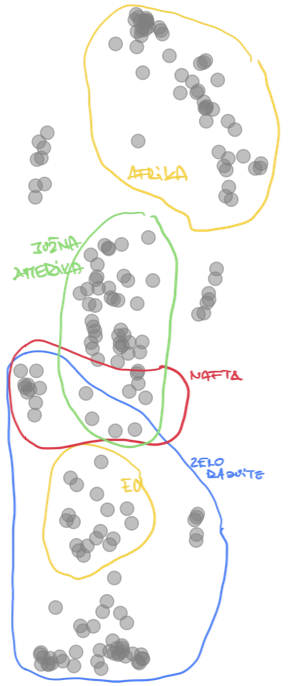
\includegraphics[width=0.8\linewidth]{figs/070-tsne-anotacija.png}
    \caption{Primer možne anotacije t-SNE razporeditve držav v dvodimenzionalno karto. Bi znali tako razlago karte sprogramirati?}
    \label{fig:tsne-anotacija}
\end{marginfigure}


V glavnem delu naše implementacije preberemo podatke o izboru, podatke o skupinah držav, izračunamo obogatenost in izpišemo rezultate:
\vspace*{3mm}
\begin{lstlisting}
import yaml
import pandas as pd

df = pd.read_excel("izbrane-države.xlsx")

all_items = set(df["Država"].astype(str).str.strip())
selected_items = set(
    df.loc[df["Izbor"] == 1, "Država"].astype(str).str.strip()
)

with open("skupine-držav.yaml", "r", encoding="utf-8") as f:
    groups = yaml.safe_load(f)

results = []
for name, group in groups.items():
    r = enrichment(all_items, selected_items, group)
    r["group"] = name
    results.append(r)

results.sort(key=lambda x: x["p_value"])

for r in results:
    print(
        f"{r['group']+":":20s} "
        f"k={r['k']:2d}, K={r['K']:2d}, "
        f"E={r['expected']:.2f}, "
        f"fold={r['fold']:.2f}, "
        f"P={r['p_value']:4f}"
    )
\end{lstlisting}

Analiza obogatenosti za naš izbor držav in skupine držav, s katerimi predstavimo domensko znanje, torej vrne po $p$-vrednosti urejen seznam skupin:
%
{\small
\begin{verbatim}
Mediteranske:        k= 4, K= 5, E=2.08, fold=1.92, P=0.0455
Evroobmočje:         k= 5, K= 9, E=3.75, fold=1.33, P=0.1591
Obmorske:            k= 5, K=10, E=4.17, fold=1.20, P=0.3182
Balkanske:           k= 1, K= 2, E=0.83, fold=1.20, P=0.6818
Zahodnoevropske:     k= 1, K= 5, E=2.08, fold=0.48, P=0.9735
\end{verbatim}
}
%
Pravzaprav nas zanimajo samo skupine, ki so statistično značilne in kjer je njihova naključna verjetnost zelo majhna. Za to pa rabimo določiti prag, 
%
\marginnote{Parameter $\alpha$ določa verjetnost napake tipa I, torej da napačno razglasimo rezultat za statistično značilen, čeprav je v resnici posledica naključja.}
%
običajno označen z $\alpha$ (npr. $\alpha = 0{,}05$), pod katerim $p$-vrednost štejemo kot dovolj majhno. Skupine z $p < \alpha$ tako obravnavamo kot obogatene, ostale pa kot posledico naključnega izbora.

Kako se potem lotim razlage morebitnih skupin s slike~\ref{fig:tsne-izbor}? Lahko z izdelavo interaktivne vizualizacije, kjer bi uporabniku omogočili izbor točk oziroma držav iz vizualizacije in potem prikazali obogatene skupine. Še boljša pa bi bila avtomatična prepoznava gruč točk na vizualizaciji in potem anotacija teh gruč z imeni obogatenih skupin. Nekaj podobnega (sicer izmišljeni) razlagi s slike~\ref{fig:tsne-anotacija}.

\begin{exercise}{Preveč skupin, premalo statistike.}
  Ustvari $100$ primerov in jih naključno razdeli v dve skupini po $50$; eno skupino obravnavaj kot izbor (\texttt{selected\_items}), drugo kot preostanek. Nato generiraj $m$ naključnih skupin (vsaka je naključna podmnožica vseh primerov) in za vsako izračunaj obogatenost z \texttt{enrichment}. Preštej, koliko skupin ima $p<0{,}05$. Ponovi za $m=100$ in $m=1000$ (z istim izborom ali z več ponovitvami). Kaj se zgodi s številom obogatenih skupin, ko povečuješ $m$?
\end{exercise}  

\section{Večkratno testiranje}

V zgornjem primeru smo testirali le nekaj skupin držav. Število skupin pa je pogosto precej večje. Države iz našega primera bi lahko bile na primer označene z mnogimi geografskimi, političnimi, gospodarskimi, kulturnimi in zgodovinskimi oznakami. Če je teh testiranih skupin veliko, se lahko zgodi, da so nekatere skupine videti statistično značilne zgolj po naključju.

Gre za {\em problem večkratnega testiranja} (angl. {\em multiple testing problem}): če izvedemo veliko ločenih testov, bodo nekateri rezultati videti statistično značilni že zaradi naklučja. Predpostavimo, da testiramo 100 skupin in uporabimo prag $\alpha = 0.05$. Tudi če nobena skupina v resnici ni obogatena, bi s to izbiro $\alpha$ zaradi naključja pričakovali približno pet skupin značilno obogatenih skupin ($p < 0.05$). Zato so lahko pri velikem številu testov izvedene vrednosti $p$ zavajajoče.

Ena najbolj znanih popravkov je te meje je Bonferronijev popravek.
%
\marginnote{Bonferronijev popravek je poimenovan po Carlu Emiliu
Bonferroniju, njegova osnova pa izhaja iz njegovega dela o verjetnostnih
neenakostih iz leta 1936.}
%
Po njem, ko izvedemo $m$ testov, prag $\alpha$ nadomestimo z
\[
\alpha' = \frac{\alpha}{m}.
\]
Bonferronijev popravek je zelo konservativen: močno zmanjša verjetnost lažnih odkritij, vendar lahko hkrati prikrije tudi nekatere dejansko obogatene skupine.

Manj konservativen in pogosto uporabnejši pristop je nadzorovanje {\em stopnje lažnih odkritij} ({\em false discovery rate}, FDR).
%
\marginnote{Stopnjo lažnih odkritij (FDR) sta leta 1995 uvedla Yoav Benjamini in Yosef Hochberg v članku ``Controlling the False Discovery Rate: A Practical and Powerful Approach to Multiple Testing'' v reviji {em Journal of the Royal Statistical Society: Series B}.}
%
FDR predstavlja pričakovani delež lažnih odkritij med vsemi rezultati, ki jih razglasimo za statistično značilne. Če na primer nadzorujemo FDR na ravni $\alpha = 0.05$, sprejmemo možnost, da je med skupinami, ki jih razglasimo za obogatene, približno $5\,\%$ lažnih odkritij. Popravek lahko razumemo kot način prilagajanja vrednosti $p$. Najprej vseh $m$ vrednosti $p$ uredimo od najmanjše do največje:
\[
p_{(1)} \le p_{(2)} \le \cdots \le p_{(m)}.
\]
Vsako urejeno vrednost $p$ nato pomnožimo s faktorjem, ki je odvisen od
njenega ranga:
\[
p_{(i)}^\ast = p_{(i)}\frac{m}{i}.
\]
Tako najmanjšo vrednost $p$ pomnožimo z $m$, drugo najmanjšo z $m/2$, tretjo z $m/3$ in tako naprej. Nato prilagojene vrednosti dodatno popravimo, da so monotono naraščajoče in se pri prehodu od manjših proti večjim izvirnim vrednostim $p$ ne zmanjšujejo. Tako dobljene prilagojene vrednosti $p$ lahko primerjamo z običajnim pragom $\alpha$. Skupine, katerih prilagojena vrednost $p$ je manjša od $\alpha$, označimo kot statistično značilne.

V primerjavi z Bonferronijevim popravkom je Benjamini--Hochbergov popravek običajno manj strog, zato pogosto odkrije več obogatenih skupin, hkrati pa še vedno omejuje pričakovani delež lažnih odkritij med prijavljenimi rezultati.

V praksi bi morala analiza obogatitve zato poročati ne le o surovih vrednostih $p$, temveč tudi o popravljenih vrednostih $p$ oziroma o oceni FDR, zlasti kadar testiramo veliko število skupin. Pri majhnem številu skupin popravek morda ne bo bistveno spremenil sklepov. Pri tisočih testiranih skupinah pa lahko popolnoma spremeni, katerim razlagam lahko zaupamo.

\section{S skupinami povezane zvezne značilke}

Vrnimo se k našemu izboru skupine držav s slike~\ref{fig:tsne-izbor}, a se tokrat osredotočimo na njihove lastnosti. Radi bi ugotovili, v katerih značilkah se izbrana skupina razlikuje od vseh drugih. V podatkih, iz katerih smo zgradili vizualizacijo, je bilo 50 značilk, zato bi bilo smiselno dobiti urejen seznam, kjer so na vrhu tiste, ki so z našim izborom najbolj povezane. Potrebujemo torej neko cenilko povezanosti skupine z informativnostjo značilke, ki zavzame večje vrednosti za značilke, pri katerih se izbrane države najbolj razlikujejo od preostalih.

Začnimo sicer s hipotetičnim primerom in za tri značilke, imenovali smo jih kar $A$, $B$, in $C$, prikažimo, kakšna je njihova porazdelitev vrednosti v izbrani množici držav in kako so te vrednosti porazdeljene v vseh ostalih državah (slika~\ref{fig:porazdelitve}). Katera značilka je najbolj informativna? Katera torej najbolje loči primere iz izbrane gruče od vseh ostalih primerov? Porazdelitvi sta ločeni pri značilkah $A$ in $B$, a je prekrivanje pri značilki $B$ manjše. Prekrivanje je veliko pri značilki $C$. 

Očitno nam o izbrani skupini
%
\marginnote{Statistiko $t$ je uvedel William Sealy Gosset leta 1908.
Objavil jo je pod psevdonimom Student v članku ``The probable error of a mean'', saj je delal za pivovarno Guinness, ki svojim zaposlenim ni dovoljevala objavljanja znanstvenih del pod lastnim imenom. Zato danes govorimo o Studentovi t-porazdelitvi in t-testu.}
%
največ informacij poda značilka $B$. Intuitivno lahko rečemo, da so boljše tiste značilke, pri katerih sta porazdelitvi čim bolj odmaknjeni druga od druge in hkrati čim manj razpršeni. Odmaknjenost lahko ocenimo z razliko med povprečnima vrednostma obeh skupin, razpršenost pa z varianco. Ker želimo eno samo cenilko, ki upošteva oboje, lahko uporabimo $t$-statistiko. Ta meri razliko med povprečjema glede na razpršenost podatkov v obeh skupinah. Za značilko $X$ jo zapišemo kot
\[
t = \frac{\bar{x}_1 - \bar{x}_2}{\sqrt{\frac{s_1^2}{n_1} + \frac{s_2^2}{n_2}}},
\]
kjer sta $\bar{x}_1$ in $\bar{x}_2$ povprečji v izbrani in preostali skupini, $s_1^2$ in $s_2^2$ varianci, $n_1$ in $n_2$ pa velikosti obeh skupin. Večja absolutna vrednost $t$ pomeni večjo ločljivost med skupinama in s tem večjo informativnost značilke.

\begin{marginfigure}
    \caption{Porazdelitev spremenljivk $A$, $B$ in $C$ v izbrani skupini primerov (oranžna) in v vseh ostalih primerih (modra).}
    \centering
    \includegraphics[width=0.7\linewidth]{figs/070-porazdelitve.pdf}
    \label{fig:porazdelitve}
\end{marginfigure}

Za rangiranje značilk bo absolutna vrednost $t$ dovolj, če pa želimo oceniti tudi statistično značilnost opažene razlike, $t$ pretvorimo v $p$-vrednost. To dobimo iz $t$-porazdelitve kot verjetnost, da bi ob predpostavki, da razlike med skupinama ni, dobili tako veliko ali še večjo vrednost $|t|$. Pri tem predpostavimo, da $t$ sledi $t$-porazdelitvi z ustreznim številom prostostnih stopenj (npr. $\nu \approx n_1 + n_2 - 2$) in izračunamo repno verjetnost. Za dvostranski test velja
\[
p = 2 \cdot P(T \ge |t|).
\]
Manjša kot je $p$-vrednost, manj verjetno je, da je opažena razlika posledica naključja. V Pythonu to izračunamo kot:

\vspace*{3mm}
\begin{lstlisting}
from scipy.stats import t
p_value = 2 * t.sf(abs(t_stat), df)
\end{lstlisting}

S kodo, ki bi primerno prebrala podatke, nam omogočila izbor neke skupine držav in potem izračunala $t$-statistiko oziroma njeno pripadajočo $p$-vrednost bi lahko dobili izpis, katerega primer je na primer spodaj:
\vspace*{3mm}
\begin{lstlisting}
0.0000 v Neenakost v življenjski dobi (%)
0.0000 v Umrljivost dojenčkov (na 1000 rojstev)
0.0006 v Mladi brez šole in zaposlitve (%)
0.0012 v Dojenčki izključno dojeni (%)
0.0014 v Neenakost v dohodku (%)
0.0294 ^ Delež žensk v parlamentu (%)
0.0769 ^ Plačan porodniški dopust (dni)
\end{lstlisting}
Ta poleg $p$-vrednosti tudi pove, ali je vrednost značilke v izbrani skupini manjša ali večja. Seveda bi bilo zelo primerno, če bi za tako analizo razvili primerni uporabniški vmesnik, ki bi nam na enostaven način omogočil raziskovanje podatkov in njihovih skupin.

\section{Kaj pa, če so spremenljivke kategorične?}

Zgornje predpostavlja, da so vse značilke zvezne. Kaj pa, če so te kategorične (recimo spol, regija ali tip države)? V tem primeru lahko namesto cenilke $t$ uporabimo $\chi^2$-statistiko, ki meri odstopanje med opaženimi in pričakovanimi frekvencami v kontingenčni tabeli.

Predpostavimo, da je med 12 državami 8 članic OECD, 4 pa niso, in da tabela podatkov (glej tabelo~\ref{tab:podatki-drzave}) vsebuje značilko, ki o tem članstvu poroča. Naj bodo v izbrani skupini petih držav, kjer so 4 članice OECD in 1 ni. Ta razmerja lahko predstavimo v kontingenčni tabeli~\ref{tab:oecd}.

\begin{margintable}
\caption{Kontingenčna tabela članstva v OECD.}
\begin{center}
\small
\begin{tabular}{lcc}
\toprule
 & Izbrane & Ostale \\
\midrule
OECD     & 4 & 4 \\
Ne-OECD  & 1 & 3 \\
\midrule
Skupaj   & 5 & 7 \\
\bottomrule
\end{tabular}
\end{center}
\label{tab:oecd}
\end{margintable}

Če članstvo v OECD z izborom ne bi bilo povezano, bi pričakovane frekvence izračunali kot
\[
E_{ij}=\frac{(\text{vsota vrstice})\cdot(\text{vsota stolpca})}{\text{skupna vsota}}.
\]

Tako za članice OECD v izbrani skupini dobimo
\[
E=\frac{8\cdot 5}{12}=3{,}33,
\]
za nečlanice OECD pa
\[
E=\frac{4\cdot 5}{12}=1{,}67.
\]

Odstopanje med opaženimi in pričakovanimi frekvencami bomo kvantitativno izmerili s statistiko \(\chi^2\), ki združuje prispevke vseh celic kontingenčne tabele. Statistiko \(\chi^2\) 
%
\marginnote{Statistiko $\chi^2$ je uvedel Karl Pearson leta 1900 in jo predstavil v članku {\em On the criterion that a given system of deviations...} kot metodo za preverjanje ujemanja med opaženimi in pričakovanimi frekvencami.
}
%
izračunamo kot
\[
\chi^2=\sum_{i,j}\frac{(O_{ij}-E_{ij})^2}{E_{ij}},
\]
kjer je \(O_{ij}\) opažena, \(E_{ij}\) pa pričakovana frekvenca. V našem primeru dobimo
\[
\chi^2 = \frac{(4-3{,}33)^2}{3{,}33}
       + \frac{(4-4{,}67)^2}{4{,}67}
       + \frac{(1-1{,}67)^2}{1{,}67}
       + \frac{(3-2{,}33)^2}{2{,}33}
\approx 0{,}69.
\]
Večja kot je vrednost \(\chi^2\), večje je odstopanje med opaženimi in pričakovanimi frekvencami, in s tem močnejša povezanost med kategorično značilko in izbrano skupino. Če želimo oceniti še statistično značilnost, vrednost \(\chi^2\) pretvorimo v \(p\)-vrednost s porazdelitvijo \(\chi^2\) z ustreznim številom prostostnih stopenj, a to načeloma smemo storiti le, če so pričakovane frekvence v vseh celicah dovolj velike (praviloma vsaj okoli 5).

V Pythonu se za izračun našega primera poslužimo naslednje kode:
\vspace*{3mm}
\begin{lstlisting}
import numpy as np
from scipy.stats import chi2_contingency

O = np.array([
    [4, 4],
    [1, 3]
])

chi2_stat, p_value, df, E = chi2_contingency(O, correction=False)
print(f"chi2 = {chi2_stat:.4f}")
print(f"p    = {p_value:.4f}")
\end{lstlisting}
%
Funkcija \texttt{chi2\_contingency} vrne vrednost \(\chi^2\), njeno pripadajočo \(p\)-vrednost, število prostostnih stopenj ter matriko pričakovanih frekvenc. Program vrne,
\vspace*{3mm}
\begin{lstlisting}
chi2 = 0.6857
p    = 0.4076
\end{lstlisting}
in lahko sklepamo, da članstvo v OECD ni značilka, ki bi bila povezana z našim izborom držav.

\section{Tudi spremenljivke lahko razvrstimo v skupine}

Razlaga skupine z rangiranjem spremenljivk zahteva seveda interpretacijo. Dobro moramo poznati pomen spremenljivk in vedeti, na kaj se te nanašajo ter interpretirati rezultate skladno z $p$-vrednostmi in vrstnim redom spremenljivk v rangu. Huh, že prejšnji stavek je precej dolg in morda kompliciran. Interpretacija torej ni enostavna.

\begin{marginfigure}
\caption{Socioekonomske značilke razvrščene v skupine.}
\label{fig:skupine-znacilk}
\footnotesize
\begin{verbatim}
Otroci in mladina:
  - Otroško delo (%)
  - Mladi brez šole in zaposlitve (%)
  - Podhranjenost otrok(%)
  - Umrljivost otrok do 5 let (na 1000)
  - Dojenčki izključno dojeni (%)
  - Dojenčki brez cepljenja (DTP) (%)
  - Dojenčki brez cepljenja (ošpice) (%)

Zdravje in neenakost:
  - Neenakost v življenjski dobi (%)
  - Indeks življenjske dobe

Gospodarska struktura:
  - Zaposleni v kmetijstvu (%)
  - Zaposleni v storitvah (%)
  - Delež mestnega prebivalstva (%)
\end{verbatim}
\end{marginfigure}

Kaj pa, če si tudi tu pomagamo z domenskim znanjem, in na primer spremenljivke uredimo v skupine? Na primer tako, kot je to prikazano na sliki~\ref{fig:skupine-znacilk}. Naš cilj je tu ugotoviti, ali so za skupino izbranih držav značilne značilke, ki pripadajo določeni skupini značilk, in potem poročamo o obogatenosti teh skupin. Pri tem združimo vse, kar smo že uvedli v tem poglavju, torej rangiranje značilk, njihov izbor (glede na neko zgornjo mejo $\alpha$ za $p$-vrednost), in izračun obogatenosti skupin značilk. Izhod postopka so torej verjetnosti, da so izbrane skupine značilk v opazovani gruči zastopane bolj, kot bi pričakovali po naključju.

V zgornjem postopku smo uvedli nov parameter, mejo $\alpha$. Temu se lahko izognemo. Namesto izračuna obogatenosti na zgornji način lahko za dano skupino značilk opazujemo, kje v seznamu rangiranih značilk se pojavljajo značilke iz te skupine. Zanimajo nas primeri, kjer je večina značilk iz skupine pri vrhu urejenega seznama (prisotnost) ali pa pri dnu (odsotnost).

Cenilka, ki jo uvedemo za tak izračun, 
%
\marginnote{Mann--Whitneyjev test in pripadajočo statistiko sta leta 1947 predlagala Henry B. Mann in Donald R. Whitney kot neparametrično alternativo $t$-testu, ki ne predpostavlja normalnosti podatkov in temelji na rangih.}
%
se imenuje Mann--Whitneyjeva statistika, ki je sicer sorodna iz strojnega učenja bolj znani površini pod ROC krivuljo (t. i. {\em area under the curve}, oz. AUC). Ta meri, kako pogosto so značilke iz dane skupine uvrščene višje od značilk izven skupine, in jo lahko interpretiramo kot verjetnost, da bo naključno izbrana značilka iz skupine rangirana višje od naključno izbrane značilke izven skupine. Vrednosti statistike blizu 1 pomenijo koncentracijo značilk na vrhu seznama, vrednosti blizu 0 na dnu, vrednost okoli $0{,}5$ pa ustreza naključni razporeditvi.

Poglejmo kratek primer. Recimo, da imamo osem rangiranih značilk,
\[
x_1,\ x_2,\ x_3,\ x_4,\ x_5,\ x_6,\ x_7,\ x_8,
\]
urejenih od najbolj do najmanj informativne. Imejmo skupino značilk
\[
G=\{x_1, x_3, x_4\},
\]
preostale značilke pa označimo z $\bar G=\{x_2, x_5, x_6, x_7, x_8\}$.

Mann--Whitneyjeva statistika primerja vse pare $(g, o)$, kjer je $g \in G$ in $o \in \bar G$, ter šteje, kolikokrat je značilka iz skupine uvrščena višje (ima manjši rang) kot značilka izven skupine. V našem primeru je takih parov $3 \cdot 5 = 15$. Število ``zmag'' skupine je
\[
U = 5 + 4 + 4 = 13,
\]
saj je $x_1$ pred vsemi petimi, $x_3$ pred štirimi (ne pa pred $x_2$), in $x_4$ prav tako pred štirimi. Število zmag normaliziramo z številom vseh možnih parov, in dobimo
\[
\mathrm{AUC}=\frac{U}{|G|\cdot |\bar G|}=\frac{13}{15}\approx 0{,}867.
\]
To pomeni, da je verjetnost, da bo naključno izbrana značilka iz skupine rangirana više od naključno izbrane značilke izven skupine približno $86{,}7\%$, kar kaže na izrazito prisotnost skupine na vrhu seznama. Implementacija AUC ima linearno kompleksnost (sprehod po urejenem seznamu), če ne upoštevamo sortiranja, lahko pa uporabimo tudi tudi implementacijo iz knjižnice \texttt{scipy.stats}:

\begin{lstlisting}
from scipy.stats import mannwhitneyu

group_ranks = [1, 3, 4]
other_ranks = [2, 5, 6, 7, 8]

U, p = mannwhitneyu(group_ranks, other_ranks, alternative="less")
auc = 1 - U / (len(group_ranks) * len(other_ranks))

print(f"U = {U}")
print(f"AUC = {auc:.3f}")
print(f"p = {p:.4f}")
\end{lstlisting}
Zgornja koda vrne tudi $p$-vrednost, ki pove, kako verjetno je, da bi tako ugoden razpored značilk dobili po naključju.

\begin{margintable}
\caption{Obogatenost skupin značilk v socioekonomskih podatkih.}
\centering
\small
\begin{tabular}{lcl}
\toprule
AUC & $p$ & Skupina \\
\midrule
1.000 & 0.0008 & zdravje\_in\_neenakost \\
0.738 & 0.0434 & neenakost \\
0.721 & 0.0321 & demografija \\
0.678 & 0.0846 & izobraževanje \\
\bottomrule
\end{tabular}
\label{tab:auc}
\end{margintable}

Možen izhod take analize bi bil seznam, kot je prikazan v tabeli~\ref{tab:auc}. Ta na primer pokaže, da so izbrane države posebne z vidika zdravja, neenakosti, demografije in izobraževanja, kar je sicer precej abstraktna, a morda primerna razlaga. Za njeno razumevanje pa vsekakor potrebujemo dodatno znanje, predvsem o tem, ali so ta področja zastopana pozitivno ali negativno in na kakšen način. 

Analiza 
%
\marginnote{Tak pristop je skladen z načeli FAIR (angl. {\em Findable, Accessible, Interoperable, Reusable}), ki poudarjajo preglednost, dostopnost in ponovno uporabnost podatkov ter analiz. Več o FAIR v Wilkinson MD in sod. (2016). The FAIR Guiding Principles for scientific data management and stewardship. {\em Scientific Data}.}
%
te vrste bi morala vključevati tudi informacijo o zaželeni smeri značilk (npr. višji BDP je boljši, nižja stopnja brezposelnosti je boljša ipd.), vse to pa bi morali smiselno vključiti v uporabniški vmesnik, ki omogoča sledljivost oziroma ``vrtanje v globino'' --- od abstraktnih rezultatov do konkretnih podatkov, s katerimi lahko pojasnimo, zakaj in kako smo do teh rezultatov prišli.
%

%
\marginnote{S to vajo preveriš, da postopki razlage gruč niso vezani na konkreten algoritem gručenja---delujejo za poljuben, tudi ročno izbran izbor. Problem je sicer tudi ta, da če je izbor naključen, se zna zgoditi, da tudi zanj najdemo pojasnilo in da bo vešč domenski ekspert tudi zanj našel ustrezno domensko razlago. Tipa: zazri se v nočno nebo in najdi strelca.}
%
\begin{exercise}{Izmisli si gručo.}
Izberi poljuben javni podatkovni nabor. Ne uporabi nobene metode gručenja: namesto tega ročno izberi 10--20 primerov, ki se ti zdijo zanimivi, in jih obravnavaj kot gručo. Nato uporabi postopke iz tega poglavja za \emph{razlago} te skupine: rangiranje atributov (zvezne značilke), analizo kategoričnih spremenljivk (npr.\ \(\chi^2\)-test) in obogatenost skupin atributov. Pri interpretaciji preveri, ali rangirane značilke povejo smiselno zgodbo, ali so obogatene skupine značilk skladne s tvojim domenskim znanjem o izbranih primerih, in ali razlage povedo kaj smiselnega. 
\end{exercise}

\begin{exercise}{Razlaga gruč na podatkih o prekinitvi dela.}
  Uporabi podatkovni nabor IBM HR Analytics Employee Attrition s Kaggle-a. Zaposlene razvrsti v gruče (npr.\ metodo voditeljev, brez ciljne spremenljivke \texttt{Attrition}). Izberi gručo in z ustreno statistiko rangiraj značilke (te so tako zvezne kot diskretne, uporabi primerne pristope), ki jo najbolj ločijo od preostalih zaposlenih. Z domenskim znanjem oblikuj vsaj tri smiselne skupine značilk (npr.\ zadovoljstvo, plače, delovne obremenitve) in za vsako izračunaj obogatenost po Mann--Whitneyjevi statistiki. Kateri domenski vidiki najbolj opisujejo izbrano gručo? Ali je razlaga skladna s tem, kar bi pričakoval od podatkov o odlivu zaposlenih?
\end{exercise}  

\section{Kaj pa gručenje?}

Zgoraj smo se razpisali o razlagah gruč in malce tudi o za to potrebnih uporabniških vmesnikih. Za slednje naj sicer pripomnimo, da so taki, ki bi zares dovoljevali odlično razlago gruč, precej redki in jih najdemo bolj v specialističnih orodjih, torej teh, ki so namenjeni analizam podatkov iz izbranih domen. A nazaj na gručenje. Predpostavili bomo, da bralec področje dobro pozna, tudi iz prejšnjih predmetov, in tu samo omenili ključne pristope. Zato tu samo podamo tabelo~\ref{tab:grucenje-skupine} glavnih pristopov, in opišemo nekaj izbranih metod.

\begin{table*}
  \caption{{\bf Glavne skupine metod gručenja.} Pregled ključnih pristopov z značilnimi metodami ter njihovimi osnovnimi prednostmi in slabostmi.}
  \vspace{2mm}
  \centering
  \small
  \renewcommand{\arraystretch}{1.3}
  \begin{tabular}{
    @{}
    >{\raggedright\arraybackslash}p{0.14\linewidth}
    >{\raggedright\arraybackslash}p{0.22\linewidth}
    >{\raggedright\arraybackslash}p{0.28\linewidth}
    >{\raggedright\arraybackslash}p{0.28\linewidth}
    @{}
  }
  \toprule
  \textbf{Skupina} &
  \textbf{Metode} &
  \textbf{Prednosti} &
  \textbf{Slabosti} \\
  \midrule
  
  \textbf{Particijske} &
  k-means, k-medoids &
  hitre, preproste, lahko za zelo veliko primerov &
  določitev $k$, občutljive na inicializacijo, sferične gruče \\
  
  \textbf{Hierarhične} &
  aglomerativno, delitveno &
  vizualizacija z dendrogramom &
  počasne, primerne samo za manjše podatke \\
  
  \textbf{Gostotne} &
  DBSCAN, OPTICS &
  gruče so poljubne oblike, obravnavajo šum, izločijo osamelce &
  močno občutljive na meta-parametre metode \\
  
  \textbf{Modelne} &
  Gaussove mešanice &
  probabilistične, primeri so lahko uvrščeni v več gruč &
  predpostavke porazdelitve podatkov, lokalni optimumi \\
  
  \textbf{Na omrežjih} &
  Louvain, Leiden &
  primerne za omrežja, skupnosti &
  odvisne od konstrukcije grafa \\
  
  \textbf{Projekcijske / vgraditvene} &
  t-SNE, PCA, spektralno gručenje &
  zaznajo lahko kompleksno strukturo, vizualizacija &
  niso neposredno namenjene iskanju gruč, potrebna je dodatna analiza \\
  
  \bottomrule
  \end{tabular}
  \label{tab:grucenje-skupine}
\end{table*}

\section{Hierarhično gručenje}

Hierarhično gručenje gradi hierarhijo gruč iz podatkov. V najpogostejši, t. im. združevalni različici vsak primer na začetku tvori
svojo lastno gručo, nato pa se gruče postopoma združujejo, dokler vsi primeri
ne pripadajo eni sami gruči. Vhod v metodo predstavlja množica primerov skupaj z:
\begin{itemize}
\item mero razdalje med primeri (npr.\ evklidska, manhattanska, kosinusna);
\item kriterijem povezovanja gruč (angl. {\em linkage criterion}), s katerimi določimo razdaljo med gručami.
\end{itemize}
%
Najbolj pogosto uporabljeni kriteriji podobnosti gruč so:
\begin{itemize}
\item najmanjša razdalja med katerim koli parom primerov
      iz obeh gruč (angl. {\em single linkage}),
\item največja razdalja med katerim koli parom primerov
      iz obeh gruč (angl. {\em complete linkage}),
\item povprečna razdalja med vsemi pari primerov
      iz obeh gruč (angl. {\em average linkage}),
\item povečanje variance znotraj gruč, ki bi nastalo
      zaradi združitve obeh gruč (t. im. {\em Wardova metoda}).
\end{itemize}

Hierhično gručenje poteka po naslednjih korakih:
\begin{enumerate}
\item Začnemo z $n$ gručami, pri čemer vsaka vsebuje natanko en primer.
\item Izračunamo razdalje med vsemi pari gruč glede na izbrani kriterij povezovanja.
\item Poiščemo gruči z najmanjšo razdaljo in ju združimo v novo gručo.
\item Posodobimo razdalje med novo gručo in vsemi preostalimi gručami.
\item Ponavljamo koraka 3--4, dokler vsi primeri ne pripadajo eni sami gruči.
\end{enumerate}

Zaporedje združevanj lahko prikažemo z {\em dendrogramom}, drevesom, v katerem listi ustrezajo primerom, notranja vozlišča pa združitvam gruč. Višina združitve označuje razdaljo, pri kateri je do združitve prišlo. Če dendrogram ``prerežemo'' na izbrani višini, dobimo razdelitev podatkov v več gruč.

Za razliko od metod, kot je na primer metoda voditeljev (glej naslednje poglavje), hierarhično gručenje ne optimizira ene same globalne ciljne funkcije. Namesto tega gradi zaporedje lokalno optimalnih združitev glede na izbrani kriterij povezovanja. Pri Wardovi metodi pa odločitev o združitvi temelji na minimizaciji povečanja vsote kvadratov odstopanj znotraj gruč.

Glavna prednost hierarhičnega gručenja je, da števila gruč ni treba določiti vnaprej, hkrati pa omogoča jasno hierarhično predstavitev podatkov. Poleg tega lahko razkrije strukturo gruč na različnih ravneh podrobnosti. Njegove slabosti so razmeroma visoka računska zahtevnost ter občutljivost na izbiro mere razdalje, kriterija povezovanja in skaliranja atributov.

\section{Metoda voditeljev}
Metoda voditeljev (k-means) 
%
\marginnote{Metodo voditeljev je v danes znani obliki predstavil James MacQueen
leta 1967 v prispevku {\em Some Methods for Classification and Analysis of
Multivariate Observations}, objavljenem v zborniku {\em Fifth Berkeley
Symposium on Mathematical Statistics and Probability}.}
%
je particijska metoda gručenja, ki podatke razdeli v vnaprej določeno število $K$ gruč. Vsako gručo predstavlja njen voditelj, to je centroid oziroma povprečni vektor primerov v gruči. Vhod v metodo je množica primerov, opisanih s številskimi atributi, izbrano število gruč $K$ in mera razdalje (najpogosteje evklidska). Algoritem začne z izbiro začetnih voditeljev, nato pa iterativno ponavlja dva koraka: vsak primer priredi najbližjemu voditelju, nato pa voditelje posodobi kot centroidne vrednosti pripadajočih gruč. Postopek se konča, ko se razbitje ne spreminja več oziroma se spremembe ustalijo.

Izhod metode je razbitje primerov na $K$ gruč in pripadajoči voditelji. Metoda optimizira kompaktnost gruč, to je vsoto kvadratov razdalj primerov do njihovih voditeljev (SSE):
\[
\frac{1}{n}\sum_{i=1}^n \min_{k=1,\ldots,K}\|x_i-v_k\|^2 
\]
pri čemer so optimalni voditelji tudi centroidi gruč. Algoritem praviloma hitro konvergira, vendar le do lokalnega optimuma, zato je rezultat odvisen od začetne izbire voditeljev.

Prednost metode je njena učinkovitost in primernost za velike podatkovne množice, slabosti pa so potreba po vnaprejšnji določitvi $K$, občutljivost na inicializacijo in mera razdalje ter dejstvo, da metoda najbolje deluje za približno kroglaste in po velikosti primerljive gruče.

\begin{exercise}{Metoda voditeljev z gradientnim sestopom.}
  Implementiraj poenostavljeno metodo voditeljev, kjer so parametri modela koordinate voditeljev \(v_1,\ldots,v_K\). Za kriterijsko funkcijo uporabi povprečno kvadratno razdaljo vsakega primera do najbližjega voditelja,
  \[
  J(v_1,\ldots,v_K)=
  \frac{1}{n}\sum_{i=1}^n \min_{k=1,\ldots,K}\|x_i-v_k\|^2 .
  \]
  Ustvari nekaj dvodimenzionalnih podatkov z znanimi gručami, voditelje inicializiraj naključno in jih uči z gradientnim sestopom. Po nekaj korakih izriši podatke in trenutne položaje voditeljev. Primerjaj rezultat s klasičnim postopkom metode voditeljev, kjer v vsakem koraku primere najprej dodelimo najbližjemu voditelju, nato pa voditelje nastavimo na povprečja pripadajočih primerov.
\end{exercise}

\section{Silhueta}
Silhueta je cenilka kakovosti razbitja podatkov na skupine, ki hkrati upošteva kohezijo znotraj gruč in ločljivost med njimi. 
%
\marginnote{Silhuetni koeficient je predlagal Peter J. Rousseeuw leta 1987
v članku {\em Silhouettes: A graphical aid to the interpretation and
validation of cluster analysis}, objavljenem v reviji {\em Journal of
Computational and Applied Mathematics}. Kljub, ali pa morda ravno zaradi izjemne preprostosti je tehnika zelo uporabljana.}
%
Uporabimo jo lahko za oceno kakovosti razvrstitve pri danem številu skupin $K$, ali pa za izbor ustreznega $K$ pri metodah, kot sta metoda voditeljev ali hierarhično gručenje. Vhod v metodo je razbitje podatkov na skupine in izbrana mera razdalje med primeri, izhod pa je silhuetni koeficient $s$, ki zavzame vrednosti približno med $-1$ in $1$.

Silhueto izračunamo za vsak primer $x^{(i)}$ iz povprečne razdalje do vseh primerov v njegovi skupini, $a_i$, ter najmanjšo povprečno razdaljo do primerov v kateri koli drugi skupini, $b_i$. Silhueta primera je nato določena kot
\[
s_i = \frac{b_i - a_i}{\max(a_i, b_i)}.
\]
Vrednosti blizu $1$ pomenijo, da je primer dobro umeščen v svojo skupino, vrednosti okoli $0$ nakazujejo na prekrivanje skupin, negativne vrednosti pa na napačno razvrstitev.

Silhueta razbitja je povprečje silhuet vseh primerov.

Pri izbiri števila skupin izračunamo silhueto za različne vrednosti $K$ in izberemo tisto, ki daje največjo vrednost $s$. Uporabimo jo lahko tako pri hierarhičnih metodah kot pri metodi voditeljev. Pristop ne optimizira razbitja neposredno, temveč služi kot zunanja cenilka kakovosti. Njena prednost je intuitivna interpretacija in upoštevanje dveh ključnih vidikov gručenja, slabost pa občutljivost na izbrano mero razdalje ter manjša zanesljivost v primerih, kjer so razlike med možnimi razbitji majhne ali kjer gruče niso jasno ločene.

\begin{exercise}{Lov na največjo silhueto.}
Ustvari dvodimenzionalne podatke brez prave strukture (npr.\ 200 točk iz ene Gaussove porazdelitve). Za $K=2,3,\ldots,8$ izvedi metodo voditeljev, za vsako vrednost izračunaj silhueto in izberi $K$ z največjo vrednostjo. Dobljeno razbitje predstavi v razsevnem diagramu. Ali metoda kljub odsotnosti prave strukture vedno predlaga neko število gruč? Kaj to pove o silhueti kot dokazu obstoja gruč?
\end{exercise}

\section{Gručenje s tehniko DBSCAN}

DBSCAN (angl. {\em Density-Based Spatial Clustering of Applications with Noise}) 
%
\marginnote{DBSCAN so predlagali Martin Ester in sod. leta 1996 v članku, predstavljenem na konferenci {\em KDD}. Članek je pozneje na isti konferenci prejel nagrado {\em Test of Time Award} za izjemen vpliv na področju podatkovnega rudarjenja.}
%
poišče območja v podatkovnem prostoru, kjer je veliko primerov. Za razliko od metode voditeljev nam tu ni potrebno vnaprej določiti števila gruč, a je metode namesto tega odvisna od dveh kritičnih parametrov: polmera $\varepsilon$, ki opredeljuje okolico primera, in $minPts$, ki poda najmanjše število primerov, ki morajo biti v tej okolici, da območje štejemo za gosto.

Za primer $x$ naj bo $N_\varepsilon(x)$ množica primerov, katerih razdalja od $x$ je največ $\varepsilon$. DBSCAN razlikuje med tremi vrstami primerov:
\begin{itemize}
\item {\em jedrna točka} ({\em core point}), za katero velja $|N_\varepsilon(x)| \ge minPts$;
\item {\em robna točka} ({\em border point}), ki ni jedrna točka, vendar leži v okolici jedrne točke;
\item {\em osamelec} oziroma {\em šumna točka} ({\em outlier}, {\em noise point}), ki ni ne jedrna ne robna točka.
\end{itemize}

Postopek iskanja gruč z algortmom DBSCAN je naslednji:
\begin{enumerate}
\item Za vsak primer $x$ izračunamo njegovo $\varepsilon$-okolico $N_\varepsilon(x)$.
\item Primer $x$ označimo kot {\em jedrno točko}, če velja $|N_\varepsilon(x)| \ge minPts$.
\item Iz jedrnih točk zgradimo gruče. Začnemo z eno jedrno točko in jo postavimo v novo gručo. Nato dodamo vse jedrne točke, ki so od katere koli jedrne točke v gruči oddaljene največ $\varepsilon$. Postopek ponavljamo, dokler v gručo ne moremo dodati nobene nove jedrne točke. Nato začnemo novo gručo iz druge še neuporabljene jedrne točke.
\item Vsako nejedrno točko dodamo v gručo, če leži znotraj razdalje $\varepsilon$ od jedrne točke te gruče. Takšne točke imenujemo {\em robne točke}.
\item Točke, ki niso ne jedrne ne robne, označimo kot {\em šum}.
\end{enumerate}

DBSCAN lahko odkrije gruče nepravilnih oblik in prepozna osamelce. Glavna slabost te tehnike pa je velika občutljivost rezultatov na izbor parametrov $\varepsilon$ in $minPts$: če je $\varepsilon$ premajhen, tehnika veliko točk prepozna kot osamelce, če je prevelik, pa pride do zduževanja gruč, ki bi morale ostati ločene. DBSCAN deluje slabše tudi takrat, ko imajo različni deli podatkovnega prostora zelo različne gostote.

\section{Gručenje na omrežjih}

Pri gručenju na omrežjih podatke najprej predstavimo kot graf. Vozlišča
grafa predstavljajo primere, ki so paroma povezani, če je razdalja med primeri manjša od izbranega praga. Seveda lahko to gručenje uporabljamo tudi takrat, če je graf že podan in ne izhajamo iz podatkov in nad njimi določenih mer podobnosti.

Primer preproste metoda za iskanje skupin v takem grafu je postopek razširjanja oznak (angl. {\em label propagation}):
\begin{enumerate}
\item Vsakemu vozlišču priredimo svojo oznako.
\item Vozlišča obiskujemo v nekem (naključnem) vrstnem redu.
\item Za vsako vozlišče pregledamo oznake njegovih sosedov, in oznako vozlišča zamenjamo z oznako, ki se med njegovimi sosedi pojavlja najpogosteje. Če se pri tem določene oznake pojavljajo enako pogosto, med njimi eno izberemo naključno.
\item Postopek ponavljamo, dokler se oznake vozlišč ne spreminjajo več, ali pa se oznake spremenijo le manjšemu delu vozlišč.
\end{enumerate}

\begin{exercise}{Gruče držav na mreži podobnosti}
Uporabi podatkovni nabor Human Development Index iz repozitorija Kaggle (880 značilk). Ustrezno pripravi podatke in za podobnost med državami uporabi kosinusno razdaljo na standardiziranih značilkah; kratko utemelji, zakaj je pri takšnem številu značilk ta mera smiselnejša od evklidske, lahko pa tudi primerjaš rezultate z obema značilkama. Z uporabo smiselno izbranega praga za razdaljo (predlagaj ustrezni postopek) zgradi omrežje (dve državi sta povezani, če je podobnost večja od pražne). Na omrežju izvedi gručenje z razširjanjem oznak. Prag izberi tako, da dobiš od tri do pet skupin. Rezultate lahko prikažeš na barvni karti sveta, omrežje pa lahko tudi narišeš (primerna knjižnica je na primer \texttt{networkx}). Ali so odkrite skupine smiselne z vidika geografije ali razvoja?
\end{exercise}

%
\marginnote{Louvainovo metodo so predlagali Blondel in sodelavci leta 2008
v reviji {\em Journal of Statistical Mechanics: Theory and Experiment}. Ime
je dobila po Univerzi v Louvainu. Njen najbolj znan sodobni naslednik je
Leidenski algoritem, ki so ga predlagali Traag in sodelavci leta 2019 v
reviji {\em Scientific Reports}. Ta izboljša Louvainovo metodo z dodatnim
izpopolnjevanjem skupnosti in zagotavlja bolj povezane gruče. Druge različice
te ideje prilagajajo uteženim, usmerjenim, večplastnim, časovno spreminjajočim
se ali z ločljivostnim parametrom določenim omrežjem.}
%
Vozlišča z enako končno oznako tvorijo gručo oziroma skupnost. Metoda je zelo hitra in ne zahteva, da bi število gruč določili vnaprej. Njena slabost je, da je rezultat lahko odvisen od vrstnega reda obiskovanja vozlišč in od načina reševanja neodločenih primerov, ko se več oznak pojavlja enako pogosto.

Pogosteje uporabljena metoda je metoda {\em Louvain}. Ta metoda išče skupnosti z maksimizacijo {\em modularnosti}, mere, ki je visoka, kadar je znotraj skupnosti veliko povezav, med skupnostmi pa razmeroma malo. Algoritem izmenično izvaja dva koraka:
\begin{enumerate}
\item Posamezna vozlišča premika med sosednjimi skupnostmi, kadar s tem poveča modularnost.
\item Vsako odkrito skupnost nadomesti z enim novim vozliščem in zgradi manjši graf, katerega vozlišča predstavljajo te skupnosti.
\end{enumerate}
Ta koraka se ponavljata na vedno manjših grafih, dokler postopek modularnost ne more več izboljšati.

Gručenje na omrežjih je zato uporabno takrat, ko je podobnost med primeri najbolje izražena prek njihovih medsebojnih povezav. Njegove prednosti so, da lahko odkrije skupine nepravilnih oblik in da dobro deluje na velikih grafih. Njegove slabosti pa so, da je rezultat odvisen od načina konstrukcije grafa ter, pri metodah, kot je Louvainova, od parametrov, ki vplivajo na velikost in število skupnosti.

\section{Verjetnostno gručenje}

Večina metod gručenja, ki smo jih doslej omenili, vsak primer razvrsti v natanko eno gručo. Takšno gručenje imenujemo ostro (angl. {\em crisp}) ali trdo gručenje. Pri verjetnostnem gručenju pa je rezultat drugačen: za vsak primer ocenimo verjetnost, da pripada posamezni gruči. Primerek lahko zato delno pripada več gručam hkrati.

Tipična metoda verjetnostnega gručenja je {\em model mešanice Gaussovih porazdelitev} ({\em Gaussian mixture model}). Predpostavlja, da so bili podatki generirani iz mešanice več Gaussovih porazdelitev. Vsaka Gaussova porazdelitev ustreza eni gruči. Model zato za vsako gručo vsebuje vektor povprečij, kovariančno matriko in utež, ki pove, kako pogosta je ta gruča v podatkih.

Algoritem, ki se najpogosteje uporablja za prilagajanje takšnega modela, je
algoritem pričakovanja in maksimizacije (angl. {\em expectation maximization},
EM). Kot pri metodi voditeljev moramo tudi tu izbrati število gruč $K$, nato pa je potek algoritma naslednji:
\begin{enumerate}
\item Inicializiramo parametre $K$ Gaussovih porazdelitev za naš večrazsežni prostor podatkov,
\item Za vsak primer ocenimo verjetnost, da pripada posamezni Gaussovi komponenti. To je korak pričakovanja (angl. {\em expectation step}).
\item Verjetnosti pripadnosti skupinam uporabimo kot uteži za posodobitev povprečij, kovariančnih matrik in uteži mešanice Gaussovih komponent. To je korak maksimizacije (angl. {\em maximization step}).
\item Koraka pričakovanja in maksimizacije ponavljamo, dokler se parametri ne prenehajo bistveno spreminjati.
\end{enumerate}

Rezultat ni le razdelitev podatkov na gruče, temveč tudi verjetnostna porazdelitev po gručah za vsak posamezen primer. Če potrebujemo ostro gručenje, lahko vsak primer dodelimo gruči z največjo verjetnostjo.

Prednost modelov mešanice Gaussovih porazdelitev je, da omogočajo mehkejše in informativnejše gručenje kot metode, kot na primer z metodo voditeljev. S pomočjo kovariančnih matrik lahko modelirajo tudi eliptično oblikovane gruče. Slabosti te metode pa je, damoramo število gručdoločiti vnaprej,
da je rezultat lahko odvisen od začetne (naključne) nastavive parametrov modela ter da tehnika predpostavlja, da je gruče moč dobro opisati z Gaussovimi porazdelitvami.

\section{Od gruč do razlag}

Gručenje je uporabno le, če lahko odkrite skupine tudi interpretiramo. Gruče moramo zato obravnavati kot hipoteze: nakazujejo, da nekateri primeri spadajo skupaj, vendar moramo še vedno pojasniti, zakaj.

V poglavju smo obravnavali več načinov za takšno razlago. Preverimo lahko, ali so v gruči nadpovprečno zastopane znane skupine, zvezne značilke lahko razvrstimo glede na to, kako močno ločujejo gručo od preostalih primerov, kategorične značilke lahko analiziramo s kontingenčnimi tabelami, razlage pa lahko povzamemo tudi prek skupin sorodnih spremenljivk. V vseh teh primerih je ključna uporaba domenskega znanje.

Različne metode gručenja določajo skupine na različne načine. Nekatere poiščejo razdelitve skladne z jedri gruč, druge iščejo gosta območja, nekatere delujejo na omrežjih... Očitno bodo rezultati zelo odvisni od izbranega algoritma ter izbranih parametrov tehnike gručenja. Tudi zaradi tega se gručenje ne bi smelo končati zgolj s seznamom oznak ali z vizualizacijo, marveč z razlago, kaj posamezne skupine predstavljajo.

Do razlag gruč se morda najbolj enostavno dokopljemo v interaktivnih okolju za analizo podatkov, kjer, idealno, lahko izbiramo skupine, pregledujemo značilke, pregledujemo sestavo gruč, in preko izbora tehnike gručenja in njenih parametrov opazujemo, kako se razlaga spreminja. Takšno raziskovanje podaktov pa lahko vodi tudi do izbiranja le ugodnih primerov (angl. {\em cherry-picking}), prekomernega prileganja (angl. {\em overfitting}) in pretirano priročnih interpretacij, ki so lahko podvržene subjektivnemu uporabniku orodja. Vendar je tako raziskovanje tudi postopek, kjer se pogosto porodijo dobra vprašanja, navkljub ali pa morda ravno zaradi subjektivnosti opazovalca. Zanimivost tako pogosto izvira iz načina odkrivanja in opazovanja vzorcev v podatkih, robustnost odkritij pa iz primerno uporabljenih statističnih prijemom.
\chapter{Nomogrami in posplošeni linearni modeli}

Na področju odkrivanja znanj iz podatkov gradimo modele, ki jih je treba -- z namenom razumevanja odkritih vzorcev -- ustrezno predstaviti uporabniku. Eden najučinkovitejših načinov predstavitve je grafični, saj lahko v dvodimenzionalnih vizualizacijah preprosto primerjamo vpliv (moč) različnih dejavnikov in njihove medsebojne interakcije. V preteklih poglavjih smo grafične predstavitve uporabljali predvsem za prikaz podatkovnih primerov, ne pa samih modelov, v tem poglavju pa se osredotočamo prav na grafične prikaze modelov. Pri tem se bomo omejili na modele, pri katerih so vhodne značilke med seboj linearno povezane, ter na posebno obliko njihove predstavitve, imenovano nomogrami. \marginnote{Beseda {\em nomogram} izhaja iz grških besed {\em nomos} (zakon) in {\em gramme} (črta) ter označuje grafični prikaz matematičnih zakonitosti.}

Nomograme so začeli graditi že ob koncu 18.~stoletja, če ne še prej. Njihov namen je bil predvsem poenostaviti izračun sicer kompleksnih matematičnih zvez. Nomograme so uporabljali na številnih področjih, kot so elektronika, balistika, prenos toplote, radioaktivnost, medicina, biomehanika, živilska tehnologija, inženirstvo ter fizikalne, biološke in poslovne vede. Za ilustracijo slika~\ref{fig:primeri} prikazuje nomogram za Ohmov zakon ter nomogram za izračun poti pri enakomerno pospešenem gibanju oziroma v balističnem modelu s težnostnim pospeškom.


\begin{figure*}
  \centering
  \includegraphics[width=0.48\linewidth]{figs/080-ohm.pdf}
  \hfill
  \includegraphics[width=0.48\linewidth]{figs/080-pot.pdf}

  \caption{Nomograma za Ohmov zakon ($V = IR$, levo) in za izračun poti pri enakomerno pospešenem gibanju ($d = vt - \tfrac{1}{2}gt^2$, desno).}
  \label{fig:primeri}
\end{figure*}

Nomografija je bistveno bolj pestra in zanimiva veda, kot jo bomo uporabili in predstavili v tem poglavju. 
%
\marginnote{Izjemno zanimiv in celovit pregled področja nomografije podaja članek Martínez-Pagán \& Roschier (2022) Nomography: A renewed pedagogical tool to sciences and engineering high-education studies. {\em Heliyon}, 8(6), e09731.} 
%
Osredotočili se bomo predvsem na linearne kombinacije značilk ter transformacije njihovih uteženih vsot, kot se pojavljajo v določenih napovednih modelih. Te modele označujemo s skupnim izrazom posplošeni linearni modeli (angl. generalized linear models). Čeprav temeljijo na linearnih kombinacijah vhodnih spremenljivk, so zaradi svoje robustnosti, enostavnosti interpretacije in možnosti učinkovite grafične predstavitve z nomogrami izjemno uporabni v praksi. 

Nomogrami omogočajo intuitivno pretvorbo matematičnega modela v vizualno orodje za odločanje, kar je še posebej pomembno v aplikativnih vedah, kot je medicina. Med najbolj znanimi primeri je t. i. Kattanov nomogram, ki se uporablja za napoved verjetnosti kliničnih izidov (npr. preživetja ali ponovitve bolezni) na podlagi več kliničnih dejavnikov; konkretno se pogosto uporablja za napoved 12-letne verjetnosti preživetja brez ponovitve raka prostate po kirurškem zdravljenju. Primer takšnega nomograma je prikazan na sliki~\ref{fig:kattan}, kjer posamezne vrednosti vhodnih spremenljivk prispevajo točke, katerih vsota se nato preslika v končno napovedno verjetnost.

\begin{figure}[ht]
  \centering
  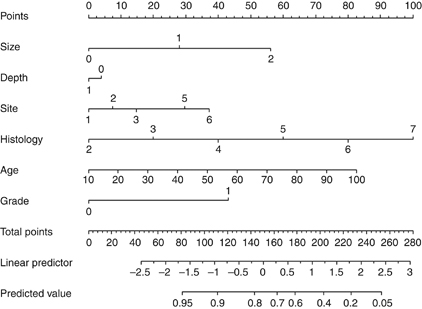
\includegraphics[width=.8\linewidth]{figs/080-kattan.jpeg}
  \caption{Pooperativni nomogram (Kattan in sod. (1999) {\em Journal of Clinical Oncology} 17(5).) za napoved 12-letne verjetnosti preživetja brez ponovitve raka prostate po radikalni prostatektomiji. Nomogram uporabimo tako, da za vsako vrednost klinične značilke odčitamo pripadajoče število točk na zgornji lestvici, točke seštejemo, nato pa skupno vsoto na spodnji lestvici preslikamo v napovedano verjetnost. Nomogram nam poleg pomoči za napoved grafično predstavi tudi pomembnost posameznih značilk.}
  \label{fig:kattan}
\end{figure}

V tem poglavju si bomo ogledali vrsto napovednih modelov, ki jih lahko učinkovito predstavimo z nomogrami, zlasti v njihovi preprostejši obliki, kot jo ponazarja Kattanov nomogram. Začnemo z linearno regresijo, nato pa preidemo na širši razred modelov, ki kljub morebitni nelinearni transformaciji ohranjajo linearno strukturo v parametrih, ter raziščemo, v kolikšni meri jih lahko enotno obravnavamo v okviru posplošenih linearnih modelov. Čeprav nomografija kot disciplina ponuja bistveno širši nabor pristopov in konstrukcij, se njena sodobna uporaba pri napovednih modelih večinoma omejuje prav na takšne, pregledne in interpretabilne oblike, ki omogočajo neposredno povezavo med vhodnimi značilkami in končno napovedjo, kot je razvidno na sliki~\ref{fig:kattan}.

\section{Nomogram za model linearne regresije}

Tole bo kar precej enostavno. Linearna regresija je utežena vsota. Vsak del utežene vsote lahko obravnavamo kot točke, ki se na koncu seštejejo in pretvorijo v končno napoved. Točkovanje lahko poenostavimo tako, da so točke celoštevilske in jih je na koncu enostavneje sešteti, vendar potrebujemo pretvorbo v končno veličino, ki pa je linearna. Primer takega nomograma prikazuje slika~\ref{fig:bodyfat} z nam že znanim primerom izračuna deleža telesnih maščob.

\begin{figure}[ht]
\centering
\includegraphics[width=\linewidth]{figs/080-lin.pdf}
\caption{Nomogram linearne regresije za izračun deleža telesnih maščob (t. i. {\em body fat Brozek}). Iz grafa je jasno razvidno, da je ključna spremenljivka obseg trebuha, veliko manjšo vlogo ima teža, medtem ko je vpliv starosti in mer bicepsa skoraj zanemarljiv. Vpliv začetne vrednosti funkcije smo upoštevali pri pretvorbi zbranih točk v vrednost razreda.}
\label{fig:bodyfat}
\end{figure}

Z nomogramom smo model grafično predstavili tako, da ga lahko sedaj uporabljamo tudi brez računalnika, zgolj z odčitavanjem in seštevanjem točk. Takšen prikaz obenem jasno poudari pomen posameznih značilk oziroma njihovo ``moč'' v modelu, saj se njihov vpliv neposredno odraža v razponu točk, ki jih prispevajo k skupni napovedi.

Postavlja se vprašanje, ali obstajajo tudi drugi, podobno enostavni modeli za nekoliko drugačne napovedne naloge, torej takšni, pri katerih značilke prav tako povežemo z uteženo vsoto, nato pa dobljeno vrednost preoblikujemo z ustrezno (nelinearno) povezovalno funkcijo, tako da lahko modeliramo tudi diskretne ali kako drugače omejene ciljne spremenljivke. V nadaljevanju začnemo s primerom takšnega modela, ki ga bomo uporabili za razvrščanje, nato pa se vprašamo, ali so tovrstne razširitve dovolj splošne za širši razred modelov, kaj pri njih pravzaprav predpostavimo, od kod izhajajo njihove kriterijske funkcije in ali gre pri tem za zanimiv razred modelov s skupnimi lastnostmi.

\section{Uvod v logistično regresijo}

Začnimo z (izmišljenim) primerom. V tabeli s slike~\ref{tab:bled} so zbrani kopalci na Bledu, ki smo jih vprašali, koliko ur na teden se ukvarjajo s športom in koliko ur so prejšnjo noč spali. Zabeležili smo tudi, ali so v dnevu intervjuvanja uspeli odplavati na otok. Ta je od bližnjega kopališča oddaljen več kot pol kilometra v eni smeri, zato je plavanje na otok in nazaj kar zalogaj, ki ne bi bil ravno primeren za slabše kopalce. Cilj je razviti aplikacijo, ki bi kopalcem svetovala, seveda glede na fizično pripravljenost in spočitost, ali naj se napotijo na tak podvig. Aplikacija seveda potrebuje napovedni model, tega pa lahko zgradimo iz naših podatkov.



\begin{marginfigure}
\caption{Primer klasifikacijskih podatkov z meta atributum, neodvisnima spremenljivkama in razredom (Otok).}
\label{tab:bled}
\footnotesize
\centering
\begin{tabular}{lccc}
\toprule
Ime & Vadba & Spanje & Otok \\
\midrule
Alenka     & 7  & 8 & 1 \\
Ana        & 2  & 8 & 0 \\
Andrej     & 5  & 5 & 0 \\
Blaž       & 5  & 9 & 1 \\
Boštjan    & 7  & 5 & 0 \\
Goran      & 12 & 6 & 1 \\
Gregor     & 10 & 9 & 1 \\
Helena     & 4  & 9 & 1 \\
Irena      & 9  & 3 & 0 \\
Janez      & 5  & 6 & 0 \\
Jure       & 8  & 4 & 0 \\
Katarina   & 4  & 3 & 0 \\
Klara      & 3  & 9 & 1 \\
Luka       & 5  & 4 & 0 \\
Maja       & 9  & 6 & 0 \\
Marko      & 4  & 7 & 0 \\
Matej      & 4  & 8 & 1 \\
Miha       & 6  & 4 & 0 \\
Mojca      & 11 & 5 & 1 \\
Nika       & 2  & 5 & 0 \\
Nina       & 8  & 6 & 1 \\
Petra      & 3  & 6 & 0 \\
Polona     & 9  & 8 & 1 \\
Rok        & 10 & 6 & 1 \\
Sara       & 6  & 7 & 1 \\
Sašo       & 10 & 7 & 1 \\
Sebastjan  & 12 & 5 & 1 \\
Tatjana    & 12 & 9 & 1 \\
Tjaša      & 11 & 3 & 0 \\
Tomaz      & 12 & 5 & 1 \\
\bottomrule
\end{tabular}
\end{marginfigure}

Ker so podatki dvodimenzionalni, jih je najbolje izrisati v razsevnem diagramu. Označimo tudi razred. Že prvi pogled na izris kaže, da je morda mogoče dobre plavalce in tiste, ki se bolj kopajo, ločiti s črto oziroma odločitveno mejo. Ta je linearna, zato jo lahko zapišemo kot $x^T\theta = 0$. Izris vključuje tudi tri nove obiskovalce: Saro, Martina in Leona. Kateremu izmed njih bo naša aplikacija oziroma model svetovala, da lahko odplava do otoka in priplava nazaj?

Sara je na strani plavalcev. Je daleč od odločitvene meje ki loči med obema razredoma. Prav gotovo lahko plava do otoka in nazaj. Martin je zelo na drugi strani, nikakor naj se ne oddalji od obale. Leon je, kar se tiče odločitvene meje, na strani plavalcev, a za las. Svetovati mu da naj poskusi plavati do otoka bi bilo zelo narobe. Naš problem je sicer klasifikacijski, želimo napovedati enega od dveh možnih razredov, a bolje bi bilo to narediti previdno, z uporabo verjetnosti. Ker je Sara zelo oddaljena od odločitvene meje, je prav gotovo kandidatka za odhod na otok, Martin nikakor ne, Leon pa je nekje na maje, njegova verjetnos ``plavalnega'' razreda je okoli 50\%.

Postaja nam jasno: oddaljenost od odločitvene meje moramo pretvoriti v verjetnosti. Kar seveda ne bo problem. Linearna kombinacija $z = x^T\theta$ je pravzaprav proporcionalna oddaljenosti od premice, ki jo določajo parametri $\theta$. Za pretvorbo lahko uporabimo funkcijo, katere zaloga vrednosti je med $0$ in $1$. Primer take funkcije je sigmoida $\sigma(z)$, naša verjetnost pa je potem
\[
P(y = 1 \mid x) = \sigma(z) = \frac{1}{1 + e^{-z}}.
\]

\begin{figure}[ht]
    \centering
    \includegraphics[width=0.8\linewidth]{figs/080-bled-scatter.pdf }
    \caption{Učni podatki, možna ločitvena meja med razredoma, in novi (imenovani) primeri, ki jih moramo še razvrstiti.}
    \label{fig:bled}
\end{figure}

\begin{marginfigure}
    \centering
    \includegraphics[width=\linewidth]{figs/080-sigmoid.pdf}
    \caption{Sigmoidna funkcija.}
    \label{fig:sigmoida}
\end{marginfigure}
%
Odločitvena meja s slike~\ref{fig:bled} ima parametre parametre $\theta_0=-15.6$, $\theta_1=0.8$ in $\theta_2=1.6$, zato lahko odločitveno enačbo za oddaljenost od te meje zapišemo kot
\[
z = -15.6 + 0.8 \cdot \text{vadba} + 1.6 \cdot \text{spanje}.
\]
Za nove primere dobimo: Sara ima $z=5.5$ in $P(\text{otok}=1)\approx 1.0$, zato je zelo primerna kandidatka za plavanje do otoka; Martin ima $z=-6.7$ in $P(\text{otok}=1)\approx 0.0$, zato mu to odsvetujemo; Leon pa ima $z=0.6$ in $P(\text{otok}=1)\approx 0.6$, kar pomeni, da je blizu odločitvene meje in je odločitev precej negotova.

Dobljeni model lahko predstavimo z nomogramom (slika~\ref{fig:bled-nnomogram}).

\begin{figure}[ht]
    \centering
    \includegraphics[width=0.8\linewidth]{figs/080-bled-nomogram.pdf }
    \caption{Nomogram za napovedovanja verjentosti plavanja na Blejski otok.}
    \label{fig:bled-nnomogram}
\end{figure}

Dobljeni model lahko predstavimo z nomogramom (slika~\ref{fig:bled-nnomogram}). Pri tem vsakemu vhodnemu atributu (vadba, spanje) priredimo svojo lestvico, na kateri posamezna vrednost atributa prispeva določeno število točk, sorazmerno z utežjo v linearni kombinaciji. Te točke nato seštejemo v skupni rezultat, ki ustreza vrednosti linearnega napovednega dela $z = x^T\theta$. Ker pa nas pri logistični regresiji ne zanima neposredno $z$, temveč verjetnost, se v naslednjem koraku skupni rezultat preslika še skozi sigmoidno funkcijo, kar v nomogramu običajno ponazorimo z dodatno, nelinearno lestvico na dnu grafa. Tako dobimo celovit vizualni pripomoček, ki omogoča, da brez eksplicitnega računanja najprej ocenimo prispevek posameznih dejavnikov, nato njihovo vsoto in končno še pripadajočo verjetnost razreda. Takšna predstavitev je posebej uporabna v praksi, saj združuje interpretabilnost linearnega modela z intuitivnim razumevanjem verjetnosti: uporabnik lahko neposredno vidi, kako sprememba ene spremenljivke vpliva na končni izid, hkrati pa ohrani občutek za negotovost napovedi, zlasti v bližini odločitvene meje.

Model, ki smo ga precej na hitro in morda malo površno uvedli na našem primeru se imenuje logistična regresija. Pomembno je, da tako kot linearna regresija tudi ta model uporablja linearno kombinacijo neodvisnih spremenljivk, katere rezultat pa tokrat, čisto zato, da lahko vrnemo verjetnosti, transformiramo z sigmoidno funkcijo. A postavlja se vprašanje: kako se sploh naučimo ``pravih'' parametrov našega modela, toej vektorja $\theta$? Kakšno kriterijsko funkcijo za to optimiziramo? Iz kakšnih predpostavk ta izhaja? Poznamo poleg linearne in logistične regresije še kakšne druge modele te vrste? In končno, je tudi to moč uporabiti strojno odvajanje in gradientni sestop za učenje modela?

Čas je za malce teorije.

\section{Eksponentna družina porazdelitev}

Od kod torej izhajajo modeli, kot sta linearna in logistična regresija? Kakšne predpostavke sploh pri tem naredimo o podatkih? Uberemo podoben pristop kot ga že poznamo pri linearni regresiji: namesto, da bi si izmislili kriterijsko funkcijo (npr. vsota kvadratov napak na učni množici), bomo izhajali iz verjetnostnega modela, torej modela, ki generira podatke v učno množico, in iz te predpostavke izpeljali kriterijsko funkcijo.

Razred porazdelitev, ki se za naš namen izkaže še posebej uporaben, je \emph{eksponentna družina}. Porazdelitev spada v to družino, če njeno verjetnostno funkcijo (ali gostoto) za spremenljivko $y$ lahko zapišemo v obliki
\[
p(y \mid \eta) = h(y)\,\exp\left(\eta\,T(y) - A(\eta)\right),
\]
kjer je $\eta = \eta(\theta)$ naravni parameter, $T(y)$ zadostna statistika,
$A(\eta)$ normalizacijska funkcija, $h(y)$ pa od parametra neodvisen del. Torej:
\begin{itemize}
  \item $\theta$ so parametri modela,
  \item $\eta$ je naravni parameter porazdelitve; v posplošenih linearnih modelih predpostavimo, da velja $\eta(x)=x^T\theta$, zato je model linearen v~$\eta$,
%
\marginnote{
Izpeljimo povezavo med $A(\eta)$ in pričakovano vrednostjo naključne spremenljivke $y$. Ker je integral gostote verjetnosti po definiciji enak 1, velja
\[
\int h(y)\,\exp\big(\eta T(y) - A(\eta)\big)\,dy = 1.
\]
Odvajanje zgornje enačbe po $\eta$ da
\[
\mathbb{E}[T(y)] - A'(\eta) = 0,
\]
zato
\[
\mathbb{E}[T(y)] = A'(\eta).
\]
V številnih primerih velja $T(y)=y$, zato je tedaj $A'(\eta)$ enak pričakovani vrednosti naključne spremenljivke $y$.
}
%
  \item $A(\eta)$ je normalizacijska funkcija, za katero velja $\mathbb{E}[T(y)] = A'(\eta)$,
  \item $\mu(x)=\mathbb{E}[T(y)\mid x]$ je povezana z $\eta$ prek zveze $\mu = A'(\eta)$; v primeru $T(y)=y$ to ustreza $\mathbb{E}[y \mid x]$.
\end{itemize}

Ker nas bo pri strojnem učenju zanimal logaritem verjetja, je smiselno izraz za verjetnostno funkcijo za eksponentno družino logaritmirati:
\[
\log p(y \mid \eta) = \eta T(y) - A(\eta) + \log h(y).
\]

V razdelkih, ki sledijo, si bomo ogledali tri primere porazdelitev,
ki sodijo v to družino in iz katerih izhajajo linearna, logistična
in Poissonova regresija. Vsak primer bomo analizirali v naslednjih korakih:

\begin{enumerate}
\item \textbf{Privzeta porazdelitev}: zapišemo verjetnostno porazdelitev
      za naključno spremenljivko $y$ (oziroma njen logaritem) ter jo
      preuredimo v obliko eksponentne družine,

\item \textbf{Pričakovana vrednost}: izračunamo pričakovano vrednost
      \[
      \mu(x)=\mathbb{E}[y\mid x],
      \]
      in preverimo, da se ujema z zvezo $\mu = A'(\eta)$. Ta korak bi
      sicer lahko pri spodnji obravnavi posameznih modelov tudi
      izpustili, vendar se ga splača izvesti, saj nam pomaga bolje
      razumeti entitete, ki nastopajo v eksponentni družini, hkrati pa
      se ob tem spomnimo tudi izrazov za pričakovano vrednost pri
      posameznih porazdelitvah.

\item \textbf{Povezava med povprečjem in linearnim napovednikom}: 
      v tem poglavju se bomo omejili na modele, pri katerih naravni
      parameter porazdelitve določimo z linearno kombinacijo značilk,
      torej
      \[
      \eta(x)=x^T\theta.
      \]
      Nato bomo poiskali, kako je povprečna vrednost
      \[
      \mu(x)=\mathbb{E}[y\mid x]
      \]
      povezana s tem linearnim napovednikom. To zvezo opišemo s
      povezovalno funkcijo $g$, za katero velja
      \[
      g(\mu(x)) = x^T\theta.
      \]

\item \textbf{Verjetje}: zapišemo logaritemsko verjetje, iz katerega dobimo kriterijsko funkcijo za učenje modela. Ker smo v prvi točki že zapisali verjetnostno funkcijo ciljne spremenljivke, je ta korak skoraj nepotreben, a ne škodi zapisati kriterijsko funkcijo, ki jo bomo optimizirali pri učenju modela, da bo pri roki za implementacijo.
\end{enumerate}

\subsection{Verjetje in učenje modela}

Tu naj samo spomnimo, da bomo za določitev parametrov modela potrebovali kriterijsko funkcijo, za to pa potrebujemo verjetje oziroma njegov logaritem. Pravzaprav imamo za to že vse pripravljeno. Predpostavimo, da so učni primeri med seboj neodvisni, in ko se še odločimo za ciljno  porazdelitev razredov, lahko zapišemo verjetje za učne podatke
\[
p(\mathbf{y} \mid X, \theta) = \prod_{i=1}^n p(y_i \mid x_i, \theta).
\]
Za učenje parametrov maksimiziramo logaritemsko verjetje
\[
\ell(\theta) = \sum_{i=1}^n \log p(y_i \mid x_i, \theta),
\]
kar je ekvivalentno minimizaciji negativnega log-verjetja, ki ga lahko razumemo kot kriterijsko funkcijo.

Na tej točki postane povezava s strojnim učenjem očitna: različne izbire porazdelitev vodijo do različnih kriterijskih funkcij, optimizacija pa poteka enako, npr.\ z gradientnim sestopom.

\section{Linearna regresija je poseben primer eksponentne družine}

Na uporabnost eksponentne družine porazdelitev moramo šele pokazati.
Pričnimo z najpreprostejšim primerom: linearno regresijo, ki jo bomo
obdelali po zgoraj opisanih korakih.

\begin{enumerate}

\item \textbf{Privzeta porazdelitev.}
Predpostavimo, da je izhodna spremenljivka pri danih značilkah $x$
normalno porazdeljena:
\[
y \mid x \sim \mathcal{N}(\mu(x), \sigma^2),
\]
z gostoto
\[
p(y \mid x) = \frac{1}{\sqrt{2\pi\sigma^2}}
\exp\!\left(-\frac{(y - \mu(x))^2}{2\sigma^2}\right).
\]

Logaritem gostote je
\[
\log p(y \mid x) =
-\frac{(y - \mu)^2}{2\sigma^2}
- \frac{1}{2}\log(2\pi\sigma^2),
\]
kar po razvoju da
\[
\log p(y \mid x)
= \frac{\mu}{\sigma^2} y
- \frac{\mu^2}{2\sigma^2}
- \frac{y^2}{2\sigma^2}
- \frac{1}{2}\log(2\pi\sigma^2).
\]

To je oblike eksponentne družine
\[
\log p(y \mid \eta)
= \eta\,T(y) - A(\eta) + \log h(y),
\]
kjer prepoznamo
\[
T(y)=y, \qquad
\eta = \frac{\mu}{\sigma^2},
\]
\[
A(\eta) = \frac{\sigma^2}{2}\eta^2, \qquad
\log h(y)= -\frac{y^2}{2\sigma^2} - \frac{1}{2}\log(2\pi\sigma^2).
\]

\item \textbf{Pričakovana vrednost.}
Za eksponentno družino velja $\mathbb{E}[T(y)] = A'(\eta)$, zato
\[
\mathbb{E}[y \mid x] = A'(\eta).
\]

Ker je
\[
A(\eta) = \frac{\sigma^2}{2}\eta^2,
\]
dobimo
\[
A'(\eta) = \sigma^2 \eta.
\]

Ker velja $\eta = \frac{\mu}{\sigma^2}$, sledi
\[
A'(\eta) = \mu,
\]
torej
\[
\mu(x) = \mathbb{E}[y \mid x].
\]

\item \textbf{Povezava med $\mu$ in linearnim napovednikom.}
Iz zveze $\eta = \frac{\mu}{\sigma^2}$ (pri konstantni varianci)
sledi $\eta \propto \mu$, zato lahko $\eta$ obravnavamo kot $\mu$.
Če predpostavimo
\[
\eta(x) = x^T\theta,
\]
dobimo
\[
\mu(x) = x^T\theta,
\]
torej je povezovalna funkcija identiteta.

\item \textbf{Verjetje.}
Logaritemsko verjetje za en primer je
\[
\log p(y \mid x, \theta) =
-\frac{1}{2\sigma^2}(y - x^T\theta)^2
- \frac{1}{2}\log(2\pi\sigma^2).
\]

Logaritemsko verjetje na učni množici, kjer predpostavimo neodvisnost učnih primerov, je
\[
\ell(\theta)
=
\sum_{i=1}^n
\left[
-\frac{1}{2\sigma^2}(y_i - x_i^T\theta)^2
- \frac{1}{2}\log(2\pi\sigma^2)
\right].
\]

Drugi člen ne zavisi od $\theta$, zato ga pri optimizaciji lahko
zanemarimo. Parametre modela določimo kot
\[
\theta^*
=
\arg\min_\theta L(\theta)
=
\arg\min_\theta
\sum_{i=1}^n (y_i - x_i^T \theta)^2.
\]

\end{enumerate}


\section{Tudi logistična regresija je primer eksponentne družine}

Podobno kot pri linearni regresiji bomo tudi logistično regresijo
analizirali v okviru eksponentne družine porazdelitev.

\begin{enumerate}

\item \textbf{Privzeta porazdelitev.}
Pri binarni klasifikaciji predpostavimo, da ciljna spremenljivka
pri danih značilkah $x$ sledi Bernoullijevi porazdelitvi:
\[
y \mid x \sim \mathrm{Bernoulli}(p(x)),
\]
kjer velja $y \in \{0,1\}$ in
\[
P(y=1 \mid x) = p(x), \qquad P(y=0 \mid x) = 1 - p(x).
\]

Gostoto zapišemo kot
\[
p(y \mid x) = p^y (1-p)^{1-y}.
\]

Logaritem gostote je
\[
\log p(y \mid x) = y \log p + (1-y)\log(1-p),
\]
kar preuredimo v
\[
\log p(y \mid x)
= y \log \frac{p}{1-p} + \log(1-p).
\]

To je oblike eksponentne družine
\[
\log p(y \mid \eta)
= \eta\,T(y) - A(\eta) + \log h(y),
\]
kjer prepoznamo
\[
T(y)=y, \qquad
\eta = \log\frac{p}{1-p}.
\]

Funkcijo $A$ izrazimo kot funkcijo $\eta$:
\[
A(\eta) = \log(1 + e^\eta), \qquad h(y)=1.
\]

\item \textbf{Pričakovana vrednost.} Ker je
\[
A(\eta) = \log(1 + e^\eta),
\]
dobimo
\[
A'(\eta) = \frac{e^\eta}{1 + e^\eta}.
\]

Ker velja $\eta = \log\frac{p}{1-p}$, sledi $e^\eta = \frac{p}{1-p}$ in zato
\[
A'(\eta) = \mathbb{E}[y \mid x] = p.
\]

\item \textbf{Povezava med $\mu$ in linearnim napovednikom.}
Naravni parameter je
\[
\eta = \log \frac{p}{1-p}.
\]

Ker je $\mu = p$, dobimo povezovalno funkcijo (logit)
\[
g(\mu(x)) = \log \frac{\mu(x)}{1-\mu(x)}.
\]

Če predpostavimo
\[
\eta(x) = x^T\theta,
\]
sledi
\[
\log \frac{p(x)}{1-p(x)} = x^T\theta,
\]
od koder dobimo
\[
p(x) = \frac{1}{1 + e^{-x^T\theta}}.
\]

\item \textbf{Verjetje.}
Logaritemsko verjetje za en primer je
\[
\log p(y \mid x, \theta)
= y \log p(x) + (1-y)\log(1-p(x)).
\]

Če predpostavimo neodvisnost primerov v učni množici, je logaritemsko verjetje:
\[
\ell(\theta)
= \sum_{i=1}^n \left[
y_i \log p(x_i) + (1-y_i)\log(1-p(x_i))
\right].
\]

Parametre modela določimo z minimizacijo negativnega log-verjetja:
\[
\theta^*
=
\arg\min_\theta
\left(
-\sum_{i=1}^n \left[
y_i \log p(x_i) + (1-y_i)\log(1-p(x_i))
\right]
\right),
\]
kar ustreza kriterijski funkciji, ki jo poznamo kot križna entropija.

\end{enumerate}

\section{Poissonova regresija}

Pri številnih praktičnih problemih nas ne zanima napoved zvezne količine ali verjetnosti, temveč število dogodkov v nekem časovnem ali prostorskem intervalu. Takšni primeri so na primer število prihodov strank v trgovino na uro, število prometnih nesreč na določenem odseku ceste, število klicev v klicni center ali število pojavitev določene bolezni v populaciji. Za takšne podatke je značilno, da so nenegativna cela števila in pogosto asimetrično porazdeljeni, zato linearna regresija ni primerna: lahko bi napovedovala negativne vrednosti, poleg tega pa predpostavlja konstantno varianco, kar pri štetjih običajno ne drži (varianca pogosto narašča s povprečjem). V takih primerih je smiselno uporabiti model, ki upošteva naravo podatkov, zato uporabimo Poissonovo porazdelitev, ki je v splošnem
\[
p(y) = \frac{\lambda^y e^{-\lambda}}{y!},
\]
kjer je parameter $\lambda > 0$ intenziteta procesa, torej pričakovano število dogodkov v danem intervalu, za katerega velja
\[
\mathbb{E}[y] = \lambda.
\]

\begin{enumerate}

\item \textbf{Privzeta porazdelitev.}
Predpostavimo, da ciljna spremenljivka pri danih značilkah $x$ sledi
Poissonovi porazdelitvi:
\[
y \mid x \sim \mathrm{Poisson}(\lambda(x)),
\]
kjer velja $y \in \{0,1,2,\dots\}$ in
\[
p(y \mid x) = \frac{\lambda^y e^{-\lambda}}{y!}.
\]
Parameter $\lambda(x) > 0$ predstavlja intenziteto oziroma pričakovano število dogodkov pri danih značilkah $x$, zato velja
\[
\mu(x) = \mathbb{E}[y \mid x] = \lambda(x).
\]

Logaritem gostote je
\[
\log p(y \mid x)
= y \log \lambda - \lambda - \log(y!).
\]
in če ga primerjamo z obliko eksponentne družine
\[
\log p(y \mid \eta)
= \eta\,T(y) - A(\eta) + \log h(y),
\]
lahko prepoznamo
\[
T(y)=y, \qquad
\eta = \log \lambda.
\]

Funkcijo $A$ izrazimo kot funkcijo $\eta$:
\[
A(\eta) = e^\eta, \qquad
h(y) = \frac{1}{y!}.
\]

\item \textbf{Pričakovana vrednost.} Ker je
\[
A(\eta) = e^\eta,
\]
dobimo
\[
A'(\eta) = e^\eta.
\]

Ker velja $\eta = \log \lambda$, sledi $e^\eta = \lambda$ in zato
\[
A'(\eta) = \lambda.
\]

Torej
\[
\mu(x) = \mathbb{E}[y \mid x] = \lambda(x).
\]

\item \textbf{Povezava med $\mu$ in linearnim napovednikom.}
Naravni parameter je
\[
\eta = \log \lambda.
\]

Ker je $\mu = \lambda$, dobimo povezovalno funkcijo (log)
\[
g(\mu(x)) = \log \mu(x).
\]

Če predpostavimo
\[
\eta(x) = x^T\theta,
\]
sledi
\[
\log \lambda(x) = x^T\theta,
\]
od koder dobimo
\[
\lambda(x) = e^{x^T\theta}.
\]

\item \textbf{Verjetje.}
Logaritemsko verjetje za en primer je
\[
\log p(y \mid x, \theta)
= y x^T\theta - e^{x^T\theta} - \log(y!).
\]

Logaritemsko verjetje na učni množici, kjer predpostavimo neodvisnost primerov, je:
\[
\ell(\theta)
= \sum_{i=1}^n \left[
y_i x_i^T\theta - e^{x_i^T\theta} - \log(y_i!)
\right].
\]

Ker člen $\log(y_i!)$ ne zavisi od $\theta$, ga pri optimizaciji
lahko zanemarimo. Parametre modela zato določimo z minimizacijo
negativnega log-verjetja:
\[
\theta^*
=
\arg\min_\theta
\sum_{i=1}^n \left[
e^{x_i^T\theta} - y_i x_i^T\theta
\right].
\]

\end{enumerate}

\begin{table}[htb]
\centering
\small
\renewcommand{\arraystretch}{1.4}
\begin{tabularx}{\linewidth}{X X X X}
\toprule
Porazdelitev & Tip izhoda & Kaj modeliramo & Tipične uporabe \\
\midrule
Normalna & zvezna vrednost & simetrične zvezne meritve & linearna regresija \\
Bernoullijeva & 0/1 & verjetnost dogodka & klasifikacija \\
Poissonova & cela števila & število dogodkov & prihodi, klici, nesreče \\
Gamma & pozitivna zvezna vrednost & trajanje ali strošek & čakalni časi, zavarovanja \\
Negativna binomska & cela števila & preveč razpršena štetja & epidemiologija, biologija \\
\bottomrule
\end{tabularx}
\caption{Primeri porazdelitev v posplošenih linearnih modelih.}
\label{tab:glm}
\end{table}

\section{Kaj pa ostale porazdelitve iz eksponentne družine?}

Zgoraj opisane porazdelitve nikakor niso edine, ki jih uporabljamo pri gradnji posplošenih linearnih modelov. Poleg normalne, Bernoullijeve in Poissonove porazdelitve poznamo še vrsto drugih modelov iz eksponentne družine, ki so primerni za različne tipe podatkov in napovednih nalog. Posebej uporabne so takrat, ko ciljna spremenljivka ni zvezna, ni simetrično porazdeljena ali pa je omejena na pozitivne vrednosti oziroma števila dogodkov.

Tabela~\ref{tab:glm} podaja nekaj najpogosteje uporabljenih porazdelitev v posplošenih linearnih modelih ter tipične probleme, pri katerih jih uporabimo. Poleg treh zgoraj podrobneje obravnavanih smo vključili še porazdelitev Gamma, ki jo pogosto uporabljamo za modeliranje pozitivnih zveznih količin, kot so trajanja, čakalni časi ali stroški, ter negativno binomsko porazdelitev, ki je posebej uporabna pri modeliranju štetij z veliko razpršenostjo podatkov.

\section{Primer implementacije}

Zgornje besedilo je vključevalo veliko teorije in malo primerov. Za (bolj računalniški) premor implementirajmo logistično regresijo. Tako kot pri linearni regresiji iz prejšnjega poglavju, začnemo s razredom, ki razvije kriterijsko funkcijo nad vhodnimi podatki.

\vspace*{3mm}
\begin{lstlisting}
class LogReg:
    def __init__(self, n_inputs, reg=None, reg_strength=0.0):
        self.weights = 
          [Value(random.uniform(-1, 1), label=f"w{i}")
           for i in range(n_inputs)]
        self.b = Value(0.0, label="b")
        self.reg = reg
        self.reg_strength = reg_strength

    def linear(self, x):
        return sum(w * xi for w, xi in zip(self.weights, x)) + self.b

    def __call__(self, x):
        return self.linear(x).sigmoid()

    def parameters(self):
        return self.weights + [self.b]

    def loss(self, xs, ys):
        eps = 1e-8
        losses = []
        for x, y in zip(xs, ys):
            yhat = self(x)
            y_val = Value(float(y))
            term = -(y_val * (yhat + eps).log() + \
              (1 - y_val) * (1 - yhat + eps).log())
            losses.append(term)
        data_loss = sum(losses) / Value(len(xs))

        if self.reg == "l2" and self.reg_strength > 0:
            l2_penalty = self.reg_strength * sum(w * w for w in self.weights)
            return data_loss + l2_penalty
        return data_loss

    def __repr__(self):
        weights_str = ", ".join(f"w{i}={w.data:.3f}" \
          for i, w in enumerate(self.weights))
        return f"LogReg({weights_str}, b={self.b.data:.3f})"
\end{lstlisting}

Koda implementira logistično regresijo v duhu posplošenih linearnih modelov.
%
\marginnote{Podoben razred bi lahko zapisali tudi za Poissonovo regresijo ali druge posplošene linearne modele. Pravzaprav bi bilo smiselno definirati splošen razred za take modele, ki implementira skupno strukturo (linearni napovednik in učenje), posamezni modeli pa bi podedovali le ustrezno povezovalno funkcijo in kriterijsko funkcijo. To posplošitev prepuščamo bralcu.}
%
Metoda \texttt{linear} izračuna linearni napovednik $x^T\theta$, metoda \texttt{\_\_call\_\_} pa ga preslika skozi sigmoidno funkcijo in tako vrne verjetnost razreda. Funkcija \texttt{loss} ustreza negativnemu log-verjetju (križni entropiji), ki smo ga izpeljali zgoraj, in jo minimiziramo pri učenju modela. V implementacijo smo vključili tudi možnost regularizacije. Če izberemo L2-regularizacijo, se kriterijski funkciji prišteje kazenski člen, ki zavira prevelike vrednosti uteži in tako pomaga preprečevati prenaučenost modela.

Sledi koda za učenje, kjer smo kot funkcijo za učenje uporabili kar to že razvito in zapisano v knjižnica \texttt{agrad}:

\marginnote{Podatki za naš primer so na voljo na 
\href{https://file.biolab.si/datasets/bled-plavanje.xlsx}
{\texttt{bled-plavanje.xlsx}}.
}
%
\vspace*{3mm}
\begin{lstlisting}
df = pd.read_excel("bled-plavanje.xlsx")
feature_names = ["vadba", "spanje"]
xs = df[feature_names].values.tolist()
ys = df["otok"].astype(int).tolist()

print(df[["vadba", "spanje", "otok"]].head().to_string(index=False))

model = LogReg(n_inputs=len(feature_names), reg="l2", reg_strength=0.01)
model = train(model, xs, ys, learning_rate=0.1, n_epochs=10000, batch_size=None)
\end{lstlisting}

Optimizacija konvergira sorazmerno hitro, pridobljeni parametri pa se dobro ujemajo s tistimi iz slike~\ref{fig:bled}.

\vspace*{3mm}
\begin{lstlisting}
>>> model
LogReg(w0=0.756, w1=1.566, b=-14.822)
\end{lstlisting}

% \section{Multinomna logistična regresija}

% Logistična regresija, kot smo jo uvedli zgoraj, obravnava binarni, torej dvovrednostni klasifikacijski problem. A tipično se pri klasifikaciji s problemi, kjer je razredov več. Pri klasifikaciji slik želimo na primer določiti, kateri predmet je na sliki, pri obdelavi besedil pa napovedujemo temo dokumenta ali naslednji zlog ali besedo v stavku. V takih primerih je število možnih izhodov (veliko) večje od dveh, zato potrebujemo modele, ki znajo napovedovati porazdelitev verjetnosti čez več razredov. Eden najpogosteje uporabljenih modelov za ta namen je multinomna logistična regresija, znana tudi kot \emph{softmax regresija}, ki se zelo pogosto pojavi kot izhodna plast nevronskih mrež.

% Naj bo ciljna spremenljivka $y \in \{1,2,\dots,m\}$, kjer je $m$ število razredov. Za vsak razred $j$ definiramo linearni napovednik
% \[
% z_j = x^T \theta_j.
% \]

% Ker želimo dobiti verjetnosti, ki so nenegativne in seštejejo v~1, uporabimo funkcijo
% \[
% P(y = j \mid x) = \frac{e^{z_j}}{\sum_{l=1}^m e^{z_l}},
% \]
% ki ji pravimo \emph{softmax}. Ta funkcija preslika vektor realnih vrednosti $(z_1,\dots,z_m)$ v verjetnostni vektor.

% Model ni enolično določen, saj lahko vsem $z_j$ prištejemo isto konstanto, ne da bi se verjetnosti spremenile. Zato običajno en razred izberemo kot referenčni razred in njegov linearni napovednik nastavimo na nič:
% \[
% z_m = 0.
% \]

% Model ima tako $(m-1)$ vektorjev parametrov. Multinomna logistična regresija je posplošeni linearni model, kjer ciljna spremenljivka sledi kategorični porazdelitvi, je linearni napovednik $z_j = x^T \theta_j$, je povezovalna funkcija posplošeni logit, katere inverz je funkcija softmax.

% Model lahko zapišemo tudi kot
% \[
% y \mid x \sim \mathrm{Categorical}(p_1(x), \dots, p_m(x)),
% \]
% kjer velja
% \[
% p_j(x) = \frac{e^{x^T \theta_j}}{\sum_{l=1}^m e^{x^T \theta_l}}.
% \]

% Če imamo le dva razreda ($m=2$), se softmax poenostavi v sigmoidno funkcijo in dobimo običajno logistično regresijo. 

% Parametre modela ocenimo z maksimizacijo logaritemskega verjetja
% \[
% \ell(\theta) = \sum_{i=1}^n \log P(y_i \mid x_i),
% \]
% kar vodi do kriterijske funkcije, ki jo poznamo kot večrazredno križno entropijo. Tako kot pri logistični regresiji analitične oblike rešitve ni, zato parametre ocenjujemo numerično, npr.\ z gradientnim sestopom.

\section{Posplošeni linearni modeli in nomogrami danes}

Posplošeni linearni modeli se v praksi zelo pogosto uporabljajo, zlasti v medicini, epidemiologiji, ekonomiji in drugih aplikativnih vedah. Združujejo preprostost, interpretabilnost in dovolj veliko izrazno moč, da jih lahko uspešno uporabimo pri številnih napovednih nalogah. Pomembni so tudi zato, ker jih lahko zelo učinkovito predstavimo z nomogrami. Njihova struktura — linearna kombinacija značilk in enostavna nelinearna preslikava — omogoča neposredno pretvorbo modela v grafično orodje, kjer posamezne spremenljivke prispevajo točke, te pa vodijo do končne napovedi.

Pomembni so tudi pri oblikovanju sodobne umetne inteligence. Izhodne plasti nevronskih mrež so praviloma posplošeni linearni modeli: pri regresiji linearni model, pri dvorazredni klasifikaciji logistična regresija, pri večrazredni klasifikaciji pa multinomna logistična regresija (softmax). Podobno velja za notranje enote nevronskih mrež: vsaka najprej izračuna linearno kombinacijo vhodov, nato pa jo preslika skozi nelinearno funkcijo, kot je logistična funkcija ali njene preprostejše alternative (npr.\ ReLU). O tem več v naslednjih poglavjih.
\chapter{Nevronske mreže in poskusi razlag kompleksnih modelov}

Primer posplošenih linearnih modelov, ki smo ga obravnavali v prejšnjem poglavju, je bila logistična regresija. Ta zgradi model, katerega odločitvena meja je linearna. Oglejmo si dva primera podatkov z binarnim razredom (slika~\ref{fig:logreg}). Pri prvem primeru logistična regresija uspešno loči oba razreda, pri drugem pa popolnoma odpove. Bi lahko v drugem primeru preoblikovali prostor značilk tako, da bi logistični regresiji uspelo?


\begin{figure*}[ht]
    \centering
    \includegraphics[width=0.49\linewidth]{figs/090-logreg-line.pdf}
    \hfill
    \includegraphics[width=0.49\linewidth]{figs/090-logreg-v.pdf}
    \caption{Linearno in nelinearno ločljiva množica podatkov ter rezultat modeliranja z logistično regresijo.
    \protect\label{fig:logreg}
    }
\end{figure*}

Očitno tudi v drugi množici podatkov s slike~\ref{fig:logreg} obstajajo segmenti, kjer bi razreda lahko ločili z linearno ločnico. Če bi podatke opazoval človek, bi morda lahko začrtal dve premici in območje pod njima razglasil za področje ciljnega razreda. A za to bi morali torej postaviti dve ločeni odločitveni meji, nato pa dodati še nekaj, kar bi oddaljenost od njiju povezalo v končni klasifikator. Lahko torej na vhodu uporabimo dve logistični regresiji (za dve ločitveni meji), nato pa še eno logistično regresijo, ki združi njuna izhoda?

\section{Kombinacije logističnih regresij}

Raziščimo to zadnjo idejo kombiniranja logističnih regresij.
%
\marginnote{Opozorilo: bralec naj naše kombiniranje logističnih regresij razume predvsem kot konceptualni korak, ki nam bo omogočil razumeti nevronske mreže. V sodobnih nevronskih mrežah notranje računske enote praviloma uporabljajo enostavnejše aktivacijske funkcije, o katerih bomo govorili nekoliko kasneje.}
%
Zgradimo lahko sistem oziroma arhitekturo z dvema logističnima regresijama v vhodni plasti. Njuna izhoda označimo z $a_{00}$ in $a_{01}$, kjer prvi indeks označuje številko plasti, drugi pa številko računske enote (logistične regresije) znotraj te plasti. Ker imamo dve plasti, bi lahko aktivacijo v drugi plasti označili z $a_{10}$, a ker ta že predstavlja naš izhod $P(y=1)$, jo bomo na diagramu preprosto označili z $y$. Arhitektura takšnega sistema je prikazana na sliki~\ref{fig:three-logregs}.

\begin{marginfigure}
    \centering
    \includegraphics[width=\linewidth]{figs/090-three-logregs.pdf}
    \caption{Kombinacija treh logističnih regresij.
    \protect\label{fig:three-logregs}}
\end{marginfigure}

Naj samo spomnimo: za izračun aktivacij, to je, izhodnih vrednosti posameznih enot (torej, naših logističnih regresij) najprej izračunamo uteženo vsoto vhodov, $z = w \cdot x + b$, nato pa to vsoto pretvorimo z aktivacijsko funkcijo, to je, pri logistični regresiji z
$a = \sigma(z)$. Pri logistični regresiji smo sigmoidno preslikavo uporabili zato, da uteženo vsoto pretvorimo v verjetnost. A ker verjetnosti rabimo le na izhodu našega (kombiniranega) modela, bi lahko v vseh ostalih računskih enotah naše nastajajoče arhitekture uporabili tudi kakšne druge
%
\marginnote{Transformacijske funkcije morajo biti nelinearne. Če bi bile linearne, njihova uporaba ne bi imela smisla, saj so kombinacije linearnih funkcij še vedno linearne in bi se tako vrnili k enemu samemu računskemu vozlišču z logistično regresijo, ki ne bi moglo tvoriti nelinearnih odločitvenih mej.}
%
nelinearne transformacijske funkcije.

Predlagana arhitektura našega modela lepo reši klasifikacijski problem, kot prikazuje slika~\ref{fig:nn-v}. Ampak, ali ta res zgradi odločitvene meje tako, kot bi pričakovali? Ne povsem. Dve notranji računski vozlišči imata svoji ``odločitveni meji'' postavljeni v pričakovani smeri (slika~\ref{fig:nn-v}, desno), a zamaknjeno.

\begin{figure*}[ht]
    \centering
    \includegraphics[width=0.49\linewidth]{figs/090-nn-v.pdf}
    \hfill
    \includegraphics[width=0.49\linewidth]{figs/090-two-lines.pdf}
    \caption{Odločitvena meja in izolinije verjetnosti za celoten model (levo) in za logistični regresiji na vhodu modela (desno).
    \protect\label{fig:nn-v}
    }
\end{figure*}

Seveda bi se zmotili, če bi pričakovali, da bosta ``odločitveni meji'' obeh vhodnih logističnih regresij naše arhitekture lokalno jasno ločevali primere različnih razredov. Izhodna logistična regresija namreč uteži oddaljenosti od teh premic in jih sešteje, ne pa denimo preveri, ali sta obe oddaljenosti pozitivni (kot bi to verjetno storil človek). Zanimivo pa je, da sta ti dve premici -- in to povsem pričakovano, če o tem nekoliko premislimo -- usmerjeni pravilno in ravno prav zamaknjeni, da ju lahko uporabi končna logistična regresija. Če bi želeli, bi lahko njune uteži (ne pa tudi njunega položaja) uporabili za nadaljnjo interpretacijo modela.

\marginnote{Omenjamo ``arhitekturo modelov'', torej način, kako so računske enote, torej naše logistične regresije, med seboj povezane. Arhitekturo bomo v splošnem določili s številom plasti (nivojev) in številom računskih enot v posamezni plasti ter med enotami sosednjih plasti.}
%
Tu se seveda ne smemo ustaviti. Nadaljujemo lahko s še bolj kompleksnimi in nelinearnimi klasifikacijskimi problemi, kot je denimo ta na sliki~\ref{fig:moons}. Za te nekoliko zahtevnejše podatke smo zasnovali dve alternativni arhitekturi modelov, ki sta v osnovi ponovno le kombinaciji logističnih regresij, a obe uspeta poiskati ustrezne (in pričakovane) odločitvene meje.

\begin{figure*}[ht]
    \centering
    \includegraphics[width=0.4\linewidth]{figs/090-moons-data.pdf}
    \hfil
    \includegraphics[width=0.25\linewidth]{figs/090-nn-6.pdf}
    \hfil
    \includegraphics[width=0.33\linewidth]{figs/090-nn-4-2.pdf}
    \caption{Nekoliko kompleksnejša množica podatkov in dve različici arhitekture modela, ki bi se z njo morda lahko uspešno spopadli.
    \protect\label{fig:moons}}
\end{figure*}

Opazimo, da smo v drugi varianti arhitekture modela s slike~\ref{fig:moons} uvedli dodatno plast računskih enot. Namenoma ta plast vsebuje le dve računski enoti, saj lahko njuni aktivaciji vizualiziramo v dvorazsežnem razsevnem diagramu. Ti dve aktivaciji nato pošljemo v končno enoto, logistično regresijo, ki vrača verjetnost ciljnega razreda. Ker imajo logistične regresije linearne odločitvene meje, bi torej moral biti razred točke v prostoru aktivacij predzadnje plasti naše arhitekture linearno ločljiv. In je res (slika~\ref{fig:moons-analysis})!

\begin{figure}[ht]
    \centering
    \includegraphics[width=0.45\linewidth]{figs/090-moons-boundary.pdf}
    \hfil
    \includegraphics[width=0.45\linewidth]{figs/090-moons-activations.pdf}
    \caption{Odločitvena meja dvoplastnega modela in prostor aktivacij predzadnje plasti, ki (zaradi tega, da lahko aktivacije izrišemo v dvodimenzionalnem razsevnem diagramu) vsebuje le dve računski enoti.
    \protect\label{fig:moons-analysis}}
\end{figure}

Kombinacije logističnih regresij, ki smo jih raziskovali zgoraj, so se zgodovinsko uveljavile pod imenom {\em nevronske mreže}. Izraz je star, saj te arhitekture prvotno niso bile zasnovane kot kombinacije logističnih regresij, kot smo jih predstavili tu, temveč kot računske enote, ki naj bi posnemale nevrone v možganih. O zgodovini morda nekoliko kasneje; zdaj je čas, da ta koncept formaliziramo in zapišemo nekaj kode za njegovo implementacijo.


\section{Nevronske mreže kot postopek preoblikovanja podatkov}

Preden se poglobimo v formalizem in implementacijo nevronskih mrež, še morda precej pomembna ugotovitev: zgoraj smo na koncu naših arhitektur modelov uporabili logistično regresijo. Končni model je bil torej eden od posplošenih linearnih modelov. Vse operacije pred to računsko enoto so potem služile pripravi podatkov za ta model, torej preoblikovanju podatkov tako, da jih lahko modeliramo s posplošenim linearnim modelom.

Nevronsko mrežo torej lahko obravnavamo kot transformacijo značilk za končni, posplošeni linearni model, uporabljen na teh novih značilkah. V nasprotju z ročno pripravo podatkov, kjer bi značilke torej oblikovali ročno oziroma za njihov izračun spisali neke funkcije, se te transformacije nevronska mreža nauči hkrati s končnim modelom, v enem samem optimizacijskem postopku. Mreža tako svojo notranjo transformacijo podatkov prilagodi zadnji plasti tako, da postane končna napovedna naloga čim enostavnejša oziroma da model čim bolj ustreže neki optimizacijski funkciji.

\section{Formalni zapis nevronskih mrež}

V svoji standardni usmerjeni obliki (t. im. {\em feedforward neural network}), kjer informacije tečejo od vhodnih spremenljivk do končne plasti nevronske mreže,
%
\marginnote{Druge arhitekture nevronskih mrež, med njimi konvolucijske, rekurentne in transformerske mreže, to osnovno obliko razširjajo, a za zdaj zadošča, da začnemo z osnovno, kanonično obliko, ki jo lahko kasneje poljubno nadgradimo.}
%
je nevronska mreža parametrična funkcija \( f_{\theta} : \mathbb{R}^d \to \mathbb{R}^k \), določena kot kompozicija afinih transformacij in po komponentah uporabljenih nelinearnih aktivacijskih funkcij. Mreža je urejena po plasteh in vsebuje vhodno plast (vhodne spremenljivke), eno ali več \emph{skritih plasti} ter izhodno plast. Vsaka skrita plast vsebuje \emph{skrite enote} (ali vozlišča), katerih aktivacije niso neposredno opazovane in služijo kot vmesne predstavitve vhodnih podatkov.

Za vhod \( x \in \mathbb{R}^d \) mreža z \(L\) plastmi izračuna zaporedje aktivacij
\[
a^{(0)} = x, \qquad 
z^{(\ell)} = W^{(\ell)} a^{(\ell-1)} + b^{(\ell)}, \qquad
a^{(\ell)} = \sigma^{(\ell)}\!\left(z^{(\ell)}\right), \quad \ell = 1, \dots, L,
\]
kjer so plasti \( \ell = 1, \dots, L-1 \) skrite plasti, plast \( \ell = L \) pa izhodna plast. Pri tem sta \( W^{(\ell)} \) in \( b^{(\ell)} \) parametra (uteži in odmiki) plasti \(\ell\), \( \sigma^{(\ell)} \) so nelinearne aktivacijske funkcije, parametri celotnega modela pa so
\[
\theta = \{W^{(\ell)}, b^{(\ell)}\}_{\ell=1}^L.
\]
Končni izhod \( f_{\theta}(x) = a^{(L)} \) interpretiramo glede na nalogo, ki jo rešujemo, npr.\ kot verjetnosti pri klasifikaciji ali kot številčne vrednosti pri regresijskih problemih.

Tako kot pri vseh drugih modelih, ki smo jih doslej obravnavali, bomo tudi tu parametre modela \(\theta\) določili iz učnih podatkov z minimizacijo izbrane kriterijske funkcije \( \mathcal{L}(f_{\theta}(x), y) \), ki bo skladna z naravo problema. Tipično bomo te funkcije izbirali med temi, ki smo jih spoznali pri posplošenih linearnih modelih, ali pa uporabili njihove razširitve za zahtevnejše in bolj strukturirane tipe podatkov.

\section{Implementacija}

Računsko pretvorbo vhodnih podatkov, ki jo določa nevronska mreža, lahko predstavimo kot računski graf in ga nato uporabimo za izračun gradientov parametrov modela. Pri tem velja vse, kar smo uvedli v prejšnjih poglavjih pri bolj enostavnih modelih: v implementaciji bomo za učenje uporabili že razvito funkcijo \texttt{train}. Uporabimo lahko tudi regularizacijo, podobno kot smo jo uporabili za glajenje posplošenih linearnih modelov. Z izrazom ``implementacija'' tu zato mislimo predvsem, ali pa morda celo samo na konstrukcijo računskega grafa, ki ustreza izbrani arhitekturi nevronske mreže.

Začnimo sicer s krajšo razpravo o aktivacijskih funkcijah. V zgornjih razdelkih smo uporabljali logistično funkcijo, a v notranjih vozliščih nevronskih mrež pogosteje uporabljamo enostavnejše nelinearnosti, ki omogočajo učinkovitejše učenje in hitrejšo konvergenco k optimalnim rešitvam. Tipično se za notranja vozlišča tako namesto logistične uporablja funkcija ReLU ({\em Rectified Linear Unit}), 
\[
\text{ReLU}(z) = \max(0, z),
\]
ki vrne vhodno vrednost, če je ta pozitivna, sicer pa vrednost nič. Gre za preprosto, a zelo učinkovito nelinearno funkcijo, ki omogoča hitrejše učenje in omili problem izginjajočih gradientov ({\em vanishing gradient problem}). Do teh pride, ko se gradienti pri povratnem širjenju skozi mrežo postopoma manjšajo, kar je značilno predvsem pri sigmoidnih ali \texttt{tanh} aktivacijah. Posledično zgodnejše plasti prejmejo le izjemno šibek učni signal in se njihovi parametri posodabljajo zelo počasi. Funkcija ReLU ta problem omili, saj ima za pozitivne vhode konstanten odvod (enak \(1\)), kar omogoča učinkovitejše širjenje gradientov ter hitrejše in stabilnejše učenje. Za podporo funkciji ReLU zato razširimo našo knjižnico za avtomatsko odvajanje (razred \texttt{Value}) z njenim izračunom v smeri naprej in povratnim širjenjem gradientov:

\vspace*{3mm}
\begin{lstlisting}
def relu(self):
    out = Value(0 if self.data < 0 else self.data, (self,), 'ReLU')

    def _backward():
        self.grad += (out.data > 0) * out.grad
    out._backward = _backward

    return out
\end{lstlisting}

Nevronsko mrežo zgradimo z uporabo treh razredov: nevrona (računske enote), plasti nevronske mreže, ki vsebuje nevrone na isti ravni, ter same nevronske mreže, ki te plasti povezuje med seboj. Začnimo z osnovno računsko enoto:

\vspace*{3mm}
\begin{lstlisting}
class Neuron:

    def __init__(self, nin, activation='relu'):
        self.w = [Value(random.uniform(-1,1)) for _ in range(nin)]
        self.b = Value(0)
        self.activation = activation
        self.out = None

    def __call__(self, x):
        act = sum((wi*xi for wi,xi in zip(self.w, x)), self.b)
        out = act.sigmoid() \
           if self.activation == 'sigmoid' else act.relu()
        self.out = out
        return out

    def parameters(self):
        return self.w + [self.b]

    def __repr__(self):
        return f"Neuron({len(self.w)})"
\end{lstlisting}

Razred \texttt{Neuron} implementira nevron, ki sprejme \texttt{nin} vhodov, izračuna njihovo uteženo vsoto, prišteje začetno vrednost ter rezultat pošlje skozi aktivacijsko funkcijo, ki je privzeto ReLU. Funkcija \texttt{parameters()} vrne seznam parametrov nevrona.

Nevrone posamezne plasti povežemo v razredu \texttt{Layer}:

\vspace*{3mm}
\begin{lstlisting}
class Layer:

    def __init__(self, nin, nout, **kwargs):
        self.neurons = [Neuron(nin, **kwargs) for _ in range(nout)]

    def __call__(self, x):
        out = [n(x) for n in self.neurons]
        return out[0] if len(out) == 1 else out

    def parameters(self):
        return [p for n in self.neurons for p in n.parameters()]

    def __repr__(self):
        return f"Layer of [{', '.join(str(n) for n in self.neurons)}]"
\end{lstlisting}

Razred \texttt{Layer} predstavlja en sloj mreže, torej plasti nevronov, ki pri polno povezani mreži, kot je ta, ki jo gradimo, vsi prejmejo isti vhod. Izračun v metodi \texttt{\_\_call\_\_} pokliče vsak nevron posebej, pri čemer vsak neodvisno izračuna svojo aktivacijo. Če plast vsebuje le en nevron (torej gre za izhodni nevron), klic vrne skalar, sicer pa seznam aktivacij. Parametre plasti dobimo tako, da združimo sezname parametrov vseh njenih nevronov.

Plasti v nevronsko mrežo poveže razred \texttt{NeuralNetwork}:

\vspace*{3mm}
\begin{lstlisting}
class NeuralNetwork:

    def __init__(self, nin, nouts):
        sz = [nin] + nouts
        self.layers = [Layer(sz[i], sz[i+1], \
            activation="sigmoid" if i == len(nouts)-1 else "relu") 
            for i in range(len(nouts))]

    def __call__(self, x):
        for layer in self.layers:
            x = layer(x)
        return x

    def parameters(self):
        return [p for layer in self.layers 
            for p in layer.parameters()]

    def loss(self, X, ys):
        eps = 1e-8
        yhats = [self(x) for x in X]
        return -sum(y * (yhat + eps).log() + \
           (1-y) * (1-yhat + eps).log() \
           for y, yhat in zip(ys, yhats)) / len(ys)

    def __repr__(self):
        return f"NN of [{', '.join(str(layer) 
            for layer in self.layers)}]"
\end{lstlisting}

Razred \texttt{NeuralNetwork} zgradi mrežo tako, da njene plasti zaporedno poveže med seboj. Uporabnik poda število vhodov ter v seznamu število nevronov v posamezni skriti plasti. Vsi nevroni v skritih plasteh uporabljajo funkcijo ReLU, medtem ko zadnja plast uporablja sigmoidno funkcijo za izračun verjetnosti razredov.
%
\marginnote{Velja pripomniti, da tu gradimo klasifikacijsko nevronsko mrežo. Našo implementacijo bi bilo mogoče enostavno spremeniti za kakšno drugo, recimo regresijsko nalogo, z uporabo drugačne aktivacijske funkcije v zadnji plasti.}
%
Funkcija \texttt{\_\_call\_\_()} implementira prehod informacij v smeri naprej (angl. {\em forward pass}). Vsaka plast sprejme aktivacije prejšnje plasti in svoj izhod posreduje naslednji, dokler izhodna plast ne vrne napovedi. Mreža svoje parametre zbere iz parametrov posameznih plasti, te pa jih zberejo iz svojih nevronov. Spomnimo, da se bodo ti parametri med gradientnim sestopom posodabljali glede na njihove gradiente.

V zgornjo implementacijo smo vključili tudi funkcijo \texttt{loss} za binarno klasifikacijo, ki ustreza negativnemu log-verjetju (križni entropiji), uporabljeni pri logistični regresiji. Bralec lahko ta del implementacije brez težav prilagodi za splošnejšo uporabo ali pa določi ustrezen nadrazred, iz katerega nato izpelje modele nevronskih mrež za različne analitske naloge.

Učenje modela z dvema skritima plastema, kot smo ga uporabili za prikaz rezultatov na sliki~\ref{fig:moons-analysis}, je nato povsem preprosto:

\vspace*{3mm}
\begin{lstlisting}
n_hidden = [4, 2]
model = NeuralNetwork(2, n_hidden + [1])
train(model, X, ys, learning_rate=0.2, n_epochs=2000, 
      batch_size=50, report_every=100)
\end{lstlisting}

Konvergenca je pri tej implementaciji in naših podatkih kljub naivni implementaciji računanja gradientov razmeroma hitra. Na tem mestu velja poudariti, da je naša implementacija z uporabo knjižnice za avtomatsko odvajanje iz prejšnjih poglavij namenjena predvsem učenju in razumevanju konceptov, za resnejšo uporabo pa bomo od tu dalje posegli po zmogljivejših Pythonovih knjižnicah, kot je \texttt{pytorch}.

\section{Regularizacija}

Modeli nevronskih mrež so lahko zelo prilagodljivi in tipično imajo veliko število parametrov, zato so še posebej nagnjeni k preveliki prilagoditvi učni množici. Tako kot pri modelih, ki smo jih obravnavali v prejšnjih poglavjih, lahko tudi tu uporabimo regularizacijske tehnike, s katerimi model omejimo, da se bolje posplošuje na nove, nevidene podatke.

Neposredna razširitev regularizacije iz posplošenih linearnih modelov je uporaba kazenskih členov nad parametri modela. Najpogostejša je kazen $\ell_2$, kjer, kot že sicer vemo, kriterijski funkciji dodamo člen, sorazmeren vsoti kvadratov uteži,
\[
\mathcal{L}_{\text{reg}} = \mathcal{L} + \lambda \sum_{\ell} \|W^{(\ell)}\|_2^2,
\]
pri čemer parameter $\lambda > 0$ določa moč regularizacije. Takšna regularizacija spodbuja mrežo, da ohranja majhne uteži, kar vodi do bolj gladkih preslikav in manjše občutljivosti na šum v podatkih. Kazen $\ell_1$, ki se nam je sicer zdela zelo uporabna pri posplošenih linearnih modelih zaradi izbora značilk,
\[
\mathcal{L}_{\text{reg}} = \mathcal{L} + \lambda \sum_{\ell} \|W^{(\ell)}\|_1,
\]
spodbuja redkost (angl. {\em sparsity}), a se v nevronskih mrežah uporablja precej redkeje oziroma skoraj nikoli. Nevronske mreže se namreč običajno zanašajo na porazdeljene predstavitve, kjer se veliko majhnih prispevkov združuje v uporabne značilke, poleg tega pa lahko negladka narava kazni $\ell_1$ oteži optimizacijo.

V praksi kazen $\ell_2$ pogosto implementiramo neposredno v optimizacijskem postopku kot t. im. \emph{weight decay}. Namesto da bi regularizacijski člen eksplicitno dodali kriterijski funkciji, prilagodimo pravilo za posodobitev parametra $w$:
\[
w \leftarrow (1 - \eta \lambda)\, w - \eta \nabla_w \mathcal{L},
\]
kjer je $\eta$ hitrost učenja, z $\lambda$ pa uravnavamo stopnjo regularizacije. Tu pri vsakem koraku gradientnega sestopa uteži nekoliko skrčimo proti nič. Prav zato je {\em weight decay} standardni način implementacije regularizacije $\ell_2$ v sodobnih knjižnicah za nevronske mreže, oba izraza pa se v praksi pogosto uporabljata skoraj kot sopomenki.

Tretja pogosto uporabljena regularizacijska tehnika pa je \emph{dropout}.
%
\marginnote{Dropout so leta 2014 predlagali Srivastava, Hinton, Krizhevsky, Sutskever in Salakhutdinov v članku, objavljenem v reviji {\em Journal of Machine Learning Research}.}
%
Med učenjem vsako aktivacijo $a_i^{(\ell)}$ neodvisno nastavimo na nič z verjetnostjo $p$, z verjetnostjo $1-p$ pa jo ohranimo. To lahko zapišemo kot
\[
\tilde{a}^{(\ell)} = m^{(\ell)} \odot a^{(\ell)}, \qquad m_i^{(\ell)} \sim \text{Bernoulli}(1-p),
\]
kjer $\odot$ označuje množenje po komponentah. S tem preprečimo, da bi se mreža preveč zanašala na posamezne računske enote, in jo prisilimo, da razvije redundantne in bolj robustne notranje predstavitve. Pristop izpuščanja povezav lahko razumemo tudi kot obliko ansambelskega učenja:
%
\marginnote{Dropout se je veliko uporabljal v zgodnjem obdobju učenja nevronskih mrež (približno med letoma 2012 in 2016), danes pa je v sodobnih arhitekturah manj pogost. Še vedno je uporaben pri manjših modelih ali kadar imamo malo podatkov, medtem ko sta regularizacija z {\em weight decay} in bogatenje podatkov ({\em data augmentation}) danes običajnejša izbira.}
%
pri vsaki iteraciji dejansko učimo nekoliko drugačno podmrežo, dobljeno z odstranitvijo naključne podmnožice enot, pri čemer vse te podmreže delijo iste parametre. Končni model lahko zato razumemo kot približek povprečenja napovedi velike množice takšnih podmrež. Med uporabo modela potem uporabimo vse enote. V sodobnih implementacijah se ustrezno skaliranje običajno izvede že med učenjem (t.\ i.\ ``inverted dropout''),
%
\marginnote{Večina sodobnih knjižnic za globoko učenje, kot je PyTorch, privzeto implementira ``inverted dropout''.}
%
zato med uporabo modela niso potrebne dodatne prilagoditve.

Posebej preprosta, a učinkovita oblika regularizacije je \emph{zgodnje ustavljanje} ({\em early stopping}). Namesto da kriterijsko funkcijo na učni množici minimiziramo neomejeno dolgo, spremljamo uspešnost na validacijski množici in učenje ustavimo pri iteraciji $t^\ast$, kjer je izguba na validacijski množici $\mathcal{L}_{\text{val}}^{(t)}$ najmanjša. Po tej točki nadaljnja optimizacija običajno še zmanjšuje napako na učni množici, a povečuje napako na validacijski množici, kar kaže na prenaučenost. Zgodnje ustavljanje lahko razumemo tudi kot implicitno omejevanje norme parametrov: gradientni sestop najprej zajame grobo strukturo podatkov, šele kasneje pa začne prilagajati tudi šum. Če učenje prekinemo dovolj zgodaj, preprečimo, da bi se model preveč prilagodil učni množici in postal pretirano kompleksen. V praksi je zgodnje ustavljanje zelo enostavno implementirati in pogosto pomembno izboljša sposobnost posploševanja.

Regularizacijo lahko dosežemo tudi na ravni podatkov z \emph{bogatenjem podatkov} ({\em data augmentation}). Namesto da spreminjamo model, razširimo učno množico tako, da iz obstoječih primerov ustvarimo dodatne primere, pri čemer ohranimo njihove razrede. V dvodimenzionalni množici podatkov lahko na primer točko \(x = (2,1)\) rahlo pošumimo in ustvarimo bližnje točke, kot sta \((2.1, 1.0)\) ali \((1.9, 1.2)\), ki obdržijo isti razred. S tem predpostavimo, da majhne spremembe vhoda ne bi smele vplivati na izhod modela. Takšen postopek poveča raznolikost učnih podatkov in zmanjša težnjo modela, da bi si zapomnil posamezne primere, kar poveča robustnost in splošnost.

\section{Inicializacija in normalizacija}

Učenje nevronskih mrež z gradientnimi metodami je zelo občutljivo na velikost vhodov, izbor aktivacij in parametrov. Če teh količin ustrezno ne nadzorujemo, lahko optimizacija postane zelo počasna ali celo povsem odpove.

Preprost, a zelo učinkovit korak je normalizacija vhodnih značilk. V praksi posamezno značilko običajno standardiziramo (povprečje nič in enotska varianca). S tem zagotovimo, da so vsi vhodi na primerljivi skali, kar vodi do stabilnejših gradientov in hitrejše konvergence gradientnega sestopa.

Enako pomembna je inicializacija parametrov mreže. Če uteži inicializiramo s prevelikimi vrednostmi, lahko aktivacije med širjenjem skozi plasti hitro narastejo, kar vodi do nestabilnega obnašanja in eksplodirajočih gradientov. Če pa so uteži premajhne, se aktivacije krčijo proti nič in gradienti lahko izginejo, zaradi česar se mreža ne more učinkovito učiti. Sodobne inicializacijske sheme ta problem rešujejo tako, da začetne uteži izberejo na način, ki ohranja varianco aktivacij približno konstantno skozi vse plasti. Pogosti izbiri
%
\marginnote{Inicializacija Xavier (Glorot) iz leta 2010 postavi $\operatorname{Var}(w)=\frac{2}{n_{\text{in}}+n_{\text{out}}}$ in je primerna za sigmoidne oziroma \texttt{tanh} aktivacije. Inicializacija He (2015) uporablja $\operatorname{Var}(w)=\frac{2}{n_{\text{in}}}$, kar bolje ustreza mrežam z ReLU, kjer je približno polovica aktivacij enaka nič. Obe metodi poskušata ohraniti aktivacije in gradiente na stabilni skali skozi vse plasti ter tako izboljšati učenje.}
%
sta inicializacija Xavier (primerna za sigmoidne ali \texttt{tanh} aktivacije) ter inicializacija He (namenjena mrežam z ReLU).

V zahtevnejših primerih lahko med učenjem normaliziramo tudi vmesne aktivacije, na primer z uporabo paketne normalizacije ({\em batch normalization}). Takšne tehnike dodatno stabilizirajo optimizacijo, vendar za potrebe tega poglavja že skrbna priprava vhodnih podatkov in smiselna inicializacija zagotovita večino praktičnih koristi.


\section{Globina, širina in kapaciteta modela}

Arhitekturo nevronske mreže določata njena \emph{globina} (število plasti) in \emph{širina} (število enot v posamezni plasti). Povečevanje ene ali druge omogoča mreži predstavitev kompleksnejših funkcij. Pravzaprav lahko že mreža z eno samo skrito plastjo aproksimira poljubno zvezno funkcijo na omejenem območju, če vsebuje dovolj veliko število enot. To opažanje, pogosto imenovano \emph{lastnost univerzalne aproksimacije},
%
\marginnote{Lastnost univerzalne aproksimacije sta dokazala Cybenko (Approximation by superpositions of a sigmoidal function, {\em Mathematics of Control, Signals, and Systems}, 1989) in Hornik (Approximation capabilities of multilayer feedforward networks, {\em Neural Networks}, 1991). Dostopnejšo razlago podajajo Goodfellow in sod.\ v knjigi \emph{Deep Learning} (2016), poglavje 6.}
%
nakazuje, da globina strogo gledano ni nujna za izrazno moč modela. Vendar pa lahko takšne plitve mreže za predstavitev funkcij, ki jih globlje arhitekture opišejo precej bolj kompaktno, zahtevajo nepraktično veliko število enot.
%
\marginnote{\emph{Globoka nevronska mreža} je nevronska mreža z več kot eno skrito plastjo. Izraz ``globoka'' se nanaša na nalaganje plasti, ki modelu omogoča učenje vedno abstraktnejših predstavitev. Izraz se je uveljavil v 2000-ih letih ob ponovnem vzponu večplastnih nevronskih mrež, predvsem po zaslugi dela Geoffreyja Hintona in sodelavcev.}

Globina omogoča nevronskim mrežam gradnjo \emph{kompozicijskih predstavitev}. Vsaka plast transformira izhod prejšnje plasti in iz vhodov postopoma gradi vedno abstraktnejše značilke. Takšna hierarhična struktura pogosto vodi do učinkovitejših predstavitev: funkcije, ki bi v plitvi mreži zahtevale veliko število enot, lahko globoka mreža implementira z bistveno manj parametri. Širina pa določa bogastvo predstavitev znotraj posamezne plasti, saj mreži omogoča učenje več različnih značilk na isti ravni abstrakcije. V praksi tako k izrazni moči modela prispevata tako globina kot širina, njuno ustrezno razmerje pa je odvisno od konkretnega problema.

Skupna \emph{kapaciteta} nevronske mreže, to je, njena sposobnost aproksimacije širokega razreda funkcij, je zato določena z arhitekturo in številom parametrov. Modeli s premajhno kapaciteto bodo preenostavni (angl. {\em underfitting}) in ne bodo zajeli pomembnih vzorcev, medtem ko se lahko preveliki modeli preveč prilagodijo učni množici (angl. {\em overfitting}). Tako kot pri drugih modelih je tudi pri nevronskih mrežah nadzor kapacitete s premišljeno izbiro arhitekture in regularizacijo ključen za dobro uspešnost. V praksi izbiro primerne globine in širine pogosto vodijo eksperimentiranje, domensko znanje in uspešnost na validacijski množici, ne pa stroga teoretična pravila.

\section{Hitrost učenja in njeno prilagajanje}

Medtem ko oblika modela določa, katere funkcije lahko predstavimo, hitrost učenja v veliki meri določa, ali bomo te funkcije v praksi sploh uspeli poiskati. Tudi ob pravilno izračunanih gradientih in dobro zasnovani arhitekturi lahko neustrezno veliki koraki povsem preprečijo konvergenco. Hitrost učenja je zato eden ključnih praktičnih parametrov: tudi s pravilnimi gradienti lahko neustrezna velikost koraka prepreči uspešno učenje modela.

\emph{Hitrost učenja} $\eta$ določa velikost posodobitev parametrov. Če je prevelika, lahko optimizacija postane nestabilna in ne konvergira; če je premajhna, učenje napreduje zelo počasi ali celo obstane. Pogosta strategija je zato, da začnemo z razmeroma veliko hitrostjo učenja in jo med učenjem postopoma zmanjšujemo. Takšni postopki spreminjanja hitrosti učenja (angl. {\em learning rate schedules}), na primer stopničasto ali eksponentno zmanjševanje, omogočajo hitro začetno napredovanje in nato natančnejše prilagajanje v bližini rešitve. V praksi običajno zadostujejo že preprosti urniki v kombinaciji s spremljanjem uspešnosti na učni in validacijski množici, skrbna nastavitev hitrosti učenja pa ima pogosto večji vpliv kot bolj zapletene spremembe same arhitekture modela.

\section{Nevronske mreže s knjižnico PyTorch}

Podobno implementacijo nevronske mreže, kot smo jo ``ročno'' zgradili v tem poglavju, gradi tudi knjižnica PyTorch. Seveda na veliko bolj premišljen način, saj pri tem uporablja vektorje in večrazsežne matrike, ki jim pravimo tudi tenzorji. Za podatke iz slike~\ref{fig:nn-v} lahko v PyTorchu zgradimo model tako, da sestavimo zaporedje plasti:
%
\vspace*{3mm}
\begin{lstlisting}
import torch.nn as nn

model = nn.Sequential(
    nn.Linear(2, 2),
    nn.ReLU(),
    nn.Linear(2, 1),
    nn.Sigmoid(),
)
\end{lstlisting}
%
Prva plast \texttt{nn.Linear(2, 2)} sprejme dve vhodni značilki in izračuna dve linearni kombinaciji vhodov, torej aktivaciji dveh skritih enot. Nato funkcija \texttt{nn.ReLU()} nad njima uporabi nelinearno transformacijo. Druga linearna plast \texttt{nn.Linear(2, 1)} ti dve aktivaciji združi v eno samo vrednost, funkcija \texttt{nn.Sigmoid()} pa jo pretvori v verjetnost ciljnega razreda.

Vhodne podatke za učenje lahko preberemo iz vhodne datoteke in jih pretvorimo v tenzorje.
%
\vspace*{3mm}
\begin{lstlisting}
import pandas as pd
import torch

df = pd.read_excel(path)
y = torch.tensor(df.iloc[:, 0].astype(float).values, dtype=torch.float32).view(-1, 1)
X = torch.tensor(df.iloc[:, 1:3].astype(float).values, dtype=torch.float32)
\end{lstlisting}
%
Prvi stolpec podatkovne tabele predstavlja razred \(y\), preostala dva stolpca pa vhodni značilki \(X\). Ker PyTorch pričakuje numerične tenzorje določene oblike, podatke pretvorimo v tip \texttt{float32}, pri ciljni spremenljivki pa z \texttt{view(-1, 1)} zagotovimo obliko stolpčnega vektorja.

Za učenje moramo določiti cenovno funkcijo in optimizacijski postopek, ki bo posodabljal parametre modela glede na izračunane gradiente. 
%
\vspace*{3mm}
\begin{lstlisting}
loss_fn = nn.BCELoss()
optimizer = torch.optim.Adam(model.parameters(), lr=0.2)
\end{lstlisting}
%
Kriterijska funkcija \texttt{BCELoss} 
%
\marginnote{Namesto optimizatorja \texttt{Adam} bi lahko uporabili tudi stohastični gradientni sestop \texttt{SGD}, ki smo ga uporabljali vse do sedaj in je konceptualno preprostejši, a bomo ostali pri postopku Adam, ki zahteva manj ročnega prilagajanja hitrosti učenja.}
%
implementira nam že znano križno entropijo za binarno klasifikacijo, optimizator \texttt{Adam} pa hitrost posodabljanja parametrov prilagaja posameznim utežem in zato pogosto omogoča hitrejše ter stabilnejše učenje.


Učenje implementiramo s spodnjo kodo:
\vspace*{3mm}
\begin{lstlisting}
n_epochs = 10000

for epoch in range(n_epochs):
    y_pred = model(X)
    loss = loss_fn(y_pred, y)

    optimizer.zero_grad()
    loss.backward()
    optimizer.step()

    if epoch % 100 == 0:
        print(f"epoch {epoch:4d} | loss {loss.item():.6f}")

print(f"Final loss: {loss.item():.6f}")
\end{lstlisting}
%
Koda je sicer silno podobna tej, ki smo jo sestavili v prejšnjih poglavjih in uporabljali z našo knjižnico za strojno računanje gradientov. V vsaki iteraciji zgradimo računski graf, ga s prehodom skozi mrežo z učnimi podatki opremimo z vrednostmi izračunanih tenzorjev (spremenljivk v računskem grafu), gradiente nastavimo na nič ter s klicem \texttt{backward()} izračunamo gradiente. Nato z \texttt{optimizer.step()} posodobimo parametre modela.

\section{Onkraj polno povezanih mrež}

Nevronske mreže, ki smo jih obravnavali doslej, so bile \emph{polno povezane} oziroma goste, saj je bila vsaka enota v posamezni plasti povezana z vsemi enotami prejšnje plasti. Takšne arhitekture so zelo splošne in lahko načeloma aproksimirajo zelo širok razred funkcij. Vendar pa imajo lahko vhodni podatki v številnih aplikacijah dodatno strukturo, ki jo lahko izkoristimo za gradnjo učinkovitejših in uspešnejših modelov. Če to strukturo vključimo v arhitekturo, v model vnesemo določeno induktivno pristranost (angl. {\em inductive bias}), ki lahko pomembno izboljša učenje.

Odličen primer so \emph{konvolucijske nevronske mreže} ({\em convolutional neural networks}, CNN),
%
\marginnote{Konvolucijske nevronske mreže je v poznih osemdesetih letih predstavil Yann LeCun s sodelavci. Ena prvih uspešnih aplikacij je bila mreža LeNet-5 (1998), razvita v laboratorijih AT\&T Bell Labs in objavljena v {\em Proceedings of the IEEE}, kjer so CNN uporabili za prepoznavanje ročno pisanih števk.}
%
ki so zasnovane za podatke s prostorsko strukturo, kot so slike, ali pa za zaporedne podatke. Namesto da bi vsak vhod povezali z vsako enoto, CNN uporabljajo lokalne povezave in deljene uteži: isti majhen filter uporabijo na različnih delih vhoda. S tem zmanjšajo število parametrov in omogočijo mreži, da zaznava lokalne vzorce (na primer robove ali teksture) ne glede na njihov položaj v sliki.

Drug pomemben razred so \emph{rekurentne nevronske mreže} ({\em recurrent neural networks}, RNN),
%
\marginnote{RNN so bile prav tako predstavljene zelo zgodaj, v osemdesetih letih, med drugim v delih Johna Hopfielda (1982) ter Davida Rumelharta, Geoffreyja Hintona in Ronalda Williamsa (1986).}
%
ki so prilagojene zaporednim podatkom. Pri teh modelih izračun poteka korak za korakom, mreža pa ohranja skrito stanje, ki povzema pretekle vhode, zato so primerne za naloge, povezane s časovnimi vrstami ali besedili. V zadnjem času so pri številnih nalogah modeliranja zaporedij prevlado prevzele \emph{transformerske} arhitekture
%
\marginnote{Transformerske arhitekture so bile predlagane nedavno, uvedli so jih Vaswani in sod.\ leta 2017. Zaradi sposobnosti učinkovitega modeliranja dolgoročnih odvisnosti s pomočjo mehanizmov pozornosti ({\em attention}) in vzporednega računanja so v številnih aplikacijah, zlasti pri obdelavi naravnega jezika, večinoma nadomestile rekurentne modele.}
%
ki temeljijo na mehanizmih pozornosti ({\em attention}), s katerimi lahko model neposredno povezuje različne dele vhodnega zaporedja med seboj in tako učinkovito modelira dolgoročne odvisnosti.

Nevronske mreže pa niso omejene zgolj na napovedovanje izhodov iz vhodov, temveč jih lahko uporabimo tudi za \emph{generiranje} podatkov. Pri \emph{generativnem strojnem učenju} želimo modelirati osnovno porazdelitev podatkov tako, da lahko iz nje vzorčimo nove primere. Primeri vključujejo modele, ki generirajo realistične slike, besedila ali zvok. V to skupino sodijo arhitekture, kot so avtokodirniki ({\em autoencoders}), ki se učijo stisnjenih predstavitev s pomočjo rekonstrukcije vhodov, generativne nasprotniške mreže ({\em generative adversarial networks}, GAN) ter jezikovni modeli, temelječi na transformerskih arhitekturah. Čeprav vsi ti modeli gradijo na istih principih, ki smo jih obravnavali v tem poglavju -- kompozicijah odvedljivih funkcij, učenih z gradientno optimizacijo -- so njihovi cilji in uporabe precej širši ter danes predstavljajo samo jedro sodobne umetne inteligence.

\section{Razložljivost nevronskih mrež}

%
\marginnote{Razložljivost je danes zelo aktivno raziskovalno področje. Metode, kot so pripisovanje pomembnosti značilkam ({\em feature attribution}), zemljevidi občutljivosti ({\em saliency maps}) in analiza mehanizmov pozornosti ({\em attention analysis}), poskušajo nevronske mreže narediti bolj razumljive, zlasti v aplikacijah z visokimi tveganji.}
%
Očitno vprašanje je, ali lahko nevronske mreže interpretiramo podobno kot preprostejše modele. Pri linearnih modelih lahko razlaga modelov izhaja neposredno iz modela samega: koeficienti linearne regresije opisujejo vpliv posamezne vhodne spremenljivke na izhod. Parametri nevronske mreže pa so porazdeljeni skozi več plasti in med seboj delujejo na izrazito nelinearen način. Posamezne uteži ali enote zato praviloma nimajo preproste, samostojne interpretacije. Model moramo razumeti predvsem kot sistem, ki se uči zaporedja transformacij, s katerimi vhodne podatke preslika v predstavitev, uporabno za končno nalogo.

Vsaj delni vpogled v delovanje nevronskih mrež pa lahko dobimo z analizo njihovih napovedi, opazovanjem, kako se izhodi spreminjajo glede na vhode, ali z vizualizacijo vmesnih predstavitev, kot smo to naredili že v preprostem primeru v tem poglavju. Takšni pristopi omogočajo bolj globalno razumevanje tega, česa se je model naučil, četudi preprosta interpretacija na ravni posameznih parametrov ni na voljo.

V nadaljevanju se zato lotimo dveh pristopov. Prvi bo neposreden: z računskim grafom lahko enostavno ugotovimo, kako vhodne spremenljivke vplivajo na vrednosti izhodnih. Gradiente, izračunane iz računskega grafa, smo do sedaj uporabljali pri osveževanju vrednosti parametrov, a prav tako jih lahko izračunamo za vhodne spremenljivke in s tem dobimo informacijo, kako spremembe vhodnih spremenljivk vplivajo na izhod mreže. Drugi pristop bo namesto gradientov raje spreminjal vhode, jih ``zamajal'', in pogledal, kako se spremeni izhod. Oba pristopa bomo uporabili za razlago vpliva atributov pri izbranem primeru, nekako tako, kot bi uporabili nomogram, le da ga, prvotno, zgradimo za en sam primer. Pregled čez celoten spekter primerov lahko seveda dobimo tako, da tovrstno razlago uporabimo za vse primere v (na primer) testni množici, in tovrstne ``razlage'' grafično prikažemo v vizualizaciji, ki bo za take kompleksnejše modele nadomestila nomogram.

\section{Shapleyjeve razlage s seštevanjem prispevkov}

Pričnimo z drugo omenjeno tehniko, kjer (za zdaj) predpostavimo, da lahko uporabimo modele tako, da iz njih izključimo izbran nabor spremenljivk in naročimo modelu, da upošteva samo vse ostale spremenljivke. Začnimo s primerom. Recimo, da opazujemo ceno enosobnih stanovanj v nekem malem mestecu, kjer uporabimo model, ki pravi, da je cena odvisna od oddaljenosti stanovanja od centra, starosti stanovanja in lege (osončenost). Model smo zgradili iz podatkov, zdaj pa za novo sončno stanovanje blizu centra, za katerega je model napovedal ceno 250,000 EUR, zanima, katera vhodna spremenljivka je k tej napovedi najbolj prispevala. 

Da bi pravično ocenili prispevek vrednosti vsakega vhodnega atributa, moramo njegov prispevek opazovati v kontekstu vseh ostalih spremenljivk, to je v kontekstu koalicij. Na primer, ko nekaj o stanovanju že vemo, recimo poznamo njegovo starost, nas zanima, koliko pri oblikovanju cene stanovanja prispeva vedenje o oddaljenosti stanovanja od centra? Ali pa, če o stanovanju ne vemo še ničesar (napoved modela bi takrat morala biti enaka povprečni ceni stanovanj v naši bazi podatkov), kako se napovedana cena spremeni, če zvemo za njegovo starost? In, na primer, če že vemo, da imamo opravka z novim stanovanjem v centru mesta, kakšna je sprememba napovedane cene, če zvemo, da je lega stanovanja sončna?

Za poenostavitev notacije naše atributne vrednosti poimenujmo:
\begin{itemize}
\item A: oddaljenost (blizu centra)
\item B: starost (novo stanovanje)
\item C: lega (sončna lega)
\end{itemize}
%
Model sedaj povprašajmo po napovedi vrednosti stanovanja pri vseh možnih kombinacijah atributov. Vrednosti teh, in spremembe pri dodajanju ene od atributnih vrednosti na vhod modela, lahko predstavimo z grafom s slike~\ref{fig:lattice-one}, ki ga lahko imenujemo mreža podmnožic (angl. {\em subset lattice}) ali pa kar mreža koalicij atributov (angl. {\em Shapley coalition lattice}).
%
\marginnote{
Lloyd Shapley je leta 1953 predstavil Shapleyjeve vrednosti v članku \emph{A Value for n-Person Games}, objavljenem v zborniku \emph{Contributions to the Theory of Games II}.
}
%
V tem grafu vsako vozlišče predstavlja možno kombinacijo, oziroma koalicijo atributov na vhodu modela, prehodi v grafu pa spremembe koalicij, ko zvemo za eno dodatno vrednost atributa.

\begin{marginfigure}
    \centering
    \includegraphics[width=\linewidth]{figs/090-shap-lattice-one.pdf}
    \vspace*{-10mm}
    \caption{Mreža koalicij za model napovedovanja vrednosti nepremičnine (A: stanovanje je blizu centra, B: je novo, C: na sončni legi.)
    \protect\label{fig:lattice-one}
    }
\end{marginfigure}

Če ne vemo ničesar o stanovanju (\(\varnothing\)), je napovedana vrednost 100{,}000~€ (recimo, malo je nizka, a za primer bo zadoščalo). Če zvemo, da je stanovanje blizu centra mesta (A), se vrednost poveča na 150{,}000~€, razlika, ki nam jo prinese vedenje o tem atributu, pa je +50{,}000~€. Če po drugi strani vemo, da gre za novo stanovanje v centru mesta (AB), za katerega nam model napove, da stane 180{,}000~€, nam dodatno vedenje o njegovi sončni legi (C) prispeva k ceni 70{,}000~€.

Shapleyjeve vrednosti razdelijo razliko med napovedjo, ko poznamo vrednosti vseh atributov, in napovedjo, ko vrednosti teh atributov ne poznamo. Zanima nas sedaj, od kod razlika pri novem sončnem stanovanju v centru oziroma kateri od atributov prispeva največ k tej razliki. Ta je po Shapleyju enaka povprečni dodani vrednosti cene stanovanja v kateri koli situaciji, torej pri vseh možnih koalicijah ostalih atributnih vrednosti.

Da bi jih opazovali, poglejmo, na koliko možnih načinov se skozi mrežo koalicij sprehodimo od popolne nevednosti (ne poznamo vrednosti nobenega atributa) do situacije, ko poznamo vrednosti vseh (\(ABC\)). Vseh možnih takšnih poti je šest, kar je enako tudi številu permutacij A, B in C (\(3! = 3 \times 2 = 6\)):

\begin{enumerate}
    \item A-B-C
    \item A-C-B
    \item B-A-C
    \item B-C-A
    \item C-A-B
    \item C-B-A
\end{enumerate}

Pri vsaki permutaciji lahko zdaj izračunamo robni (marginalni) doprinos posameznega atributa, torej kolikšen je skok v ceni, ko to značilnost dodamo že obstoječi ``koaliciji'' prejšnjih.

\paragraph{Permutacija 1: A \(\rightarrow\) B \(\rightarrow\) C}

\begin{itemize}
    \item \(\varnothing \rightarrow A\) (blizu): 100{,}000 \(\rightarrow\) 150{,}000 \(\rightarrow\) +50{,}000
    \item \(A \rightarrow B\) (novo): 150{,}000 \(\rightarrow\) 180{,}000 \(\rightarrow\) +30{,}000
    \item \(A,B \rightarrow C\) (sonce): 180{,}000 \(\rightarrow\) 250{,}000 \(\rightarrow\) +70{,}000
\end{itemize}

\paragraph{Permutacija 2: A \(\rightarrow\) C \(\rightarrow\) B}

\begin{itemize}
    \item \(\varnothing \rightarrow A\) (blizu): 100{,}000 \(\rightarrow\) 150{,}000 \(\rightarrow\) +50{,}000
    \item \(A \rightarrow C\) (sonce): 150{,}000 \(\rightarrow\) 190{,}000 \(\rightarrow\) +40{,}000
    \item \(A,C \rightarrow B\) (novo): 190{,}000 \(\rightarrow\) 250{,}000 \(\rightarrow\) +60{,}000
\end{itemize}

\paragraph{Permutacija 3: B \(\rightarrow\) A \(\rightarrow\) C}

\begin{itemize}
    \item \(\varnothing \rightarrow B\) (novo): 100{,}000 \(\rightarrow\) 140{,}000 \(\rightarrow\) +40{,}000
    \item \(B \rightarrow A\) (blizu): 140{,}000 \(\rightarrow\) 180{,}000 \(\rightarrow\) +40{,}000
    \item \(A,B \rightarrow C\) (sonce): 180{,}000 \(\rightarrow\) 250{,}000 \(\rightarrow\) +70{,}000
\end{itemize}

\paragraph{Permutacija 4: B \(\rightarrow\) C \(\rightarrow\) A}

\begin{itemize}
    \item \(\varnothing \rightarrow B\) (novo): 100{,}000 \(\rightarrow\) 140{,}000 \(\rightarrow\) +40{,}000
    \item \(B \rightarrow C\) (sonce): 140{,}000 \(\rightarrow\) 200{,}000 \(\rightarrow\) +60{,}000
    \item \(B,C \rightarrow A\) (blizu): 200{,}000 \(\rightarrow\) 250{,}000 \(\rightarrow\) +50{,}000
\end{itemize}

\paragraph{Permutacija 5: C \(\rightarrow\) A \(\rightarrow\) B}

\begin{itemize}
    \item \(\varnothing \rightarrow C\) (sonce): 100{,}000 \(\rightarrow\) 160{,}000 \(\rightarrow\) +60{,}000
    \item \(C \rightarrow A\) (blizu): 160{,}000 \(\rightarrow\) 190{,}000 \(\rightarrow\) +30{,}000
    \item \(A,C \rightarrow B\) (novo): 190{,}000 \(\rightarrow\) 250{,}000 \(\rightarrow\) +60{,}000
\end{itemize}

\paragraph{Permutacija 6: C \(\rightarrow\) B \(\rightarrow\) A}

\begin{itemize}
    \item \(\varnothing \rightarrow C\) (sonce): 100{,}000 \(\rightarrow\) 160{,}000 \(\rightarrow\) +60{,}000
    \item \(C \rightarrow B\) (novo): 160{,}000 \(\rightarrow\) 200{,}000 \(\rightarrow\) +40{,}000
    \item \(B,C \rightarrow A\) (blizu): 200{,}000 \(\rightarrow\) 250{,}000 \(\rightarrow\) +50{,}000
\end{itemize}

Za vsako značilnost izračunajmo povprečni doprinos:
%
\begin{table}[h]
\centering
\begin{tabular}{ccc}
\toprule
\textbf{Značilnost} & \textbf{Prispevki po permutacijah} & \textbf{Povprečni prispevek} \\
\midrule
A & 50, 50, 40, 50, 30, 50 \(\rightarrow\) 270 & 45{,}000~€ \\
B & 30, 60, 40, 40, 60, 40 \(\rightarrow\) 270 & 45{,}000~€ \\
C & 70, 40, 70, 60, 60, 60 \(\rightarrow\) 360 & 60{,}000~€ \\
\bottomrule
\end{tabular}
\end{table}
%
Največ je torej prispevala sončna lega (C), enako pa oddaljenost od centra in starost. Prispevki se tudi (priročno) seštejejo v napovedano vrednost, kjer je ta 100{,}000~€, ko o stanovanju ne vemo ničesar, in $100{,}000 + 45{,}000 + 45{,}000 + 60{,}000 = 250{,}000$~€, ko so nam znane vse tri vrednosti vhodnih atributov.

Za vajo še en primer, kjer tokrat upoštevamo, da je stanovanje daleč od centra, na vasi (A), staro (B) in s sončno lego (C). Mrežo koalicij kaže slika~\ref{fig:lattice-two}. Ker nam je postopek zdaj znan, lahko tokrat na hitro upoštevamo vse možne poti skozi graf in ugotovimo, da so spremembe takrat, ko zvemo za A (na vasi), enake -20, -20, -40, +10, -10, +10, oziroma je povprečna sprememba enaka -11,667 €. Za starost dobimo -31,667 €, za osončeno lego pa -33,333. Od tod razlika -10,000 € v primerjavi z napovedjo modela, ko ne vemo ničesar. Stanovanje je torej cenejše kot povprečno stanovanje, najbolj pa mu ceno zmanjšuje starost.

\begin{marginfigure}
    \centering
    \includegraphics[width=\linewidth]{figs/090-shap-lattice-two.pdf}
    \vspace*{-10mm}
    \caption{Mreža koalicij za model napovedovanja vrednosti starega (B), a lepo sončnega (C) stanovanja na vasi (A).
    \protect\label{fig:lattice-two}
    }
\end{marginfigure}

\section{Shapleyjeve razlage za modele strojnega učenja}

Kako zgornjo idejo Shapleyjevih razlag uporabimo v strojnem učenju? Problem je, da vsi modeli, ki smo jih gradili do sedaj, potrebujejo vrednosti vseh vhodnih spremenljivk za njihovo delovanje. Pri Shapleyjevih vrednostih pa moramo model večkrat vprašati po napovedi tudi takrat, ko poznamo le podmnožico atributov. V praksi spremenljivke ``odstranimo'' tako, da jih nadomestimo z njihovimi pričakovanimi vrednostmi oziroma opazujemo napoved modela pri različnih vrednostih, katerih porazdelitev dobimo iz učne množice.  Postopek je sicer računsko zahteven, saj moramo za dano koalicijo model uporabiti mnogokrat, da lahko ocenimo povprečno vrednost modela pri dani koaliciji in različnih ``manjkajočih'' vrednostih atributov. Dodaten problem predstavlja tudi eksponentna rast števila koalicij s številom atributov. V praksi zato uporabljamo različne približke in optimizacije, kot so vzorčenje permutacij, aproksimacije z lokalnimi modeli ali pa posebni algoritmi za posamezne vrste modelov (na primer drevesa odločanja), kjer lahko Shapleyjeve vrednosti izračunamo bistveno hitreje.

Oglejmo si primer uporabe te tehnike pri napovedovanju deleža telesne maščobe moških.
\marginnote{Podatki so na voljo \href{https://file.biolab.si/datasets}.} Podatke bomo prebrali, jih preoblikovali za uporabo s knjižnico PyTorch, si zapomnili imena atributov in razdelili na učno in testno množico:
\vspace*{3mm}
\begin{lstlisting}
import pandas as pd

d = pd.read_excel("body-fat-brozek.xlsx")
y = torch.tensor(d.iloc[:, 0].values, dtype=torch.float32).view(-1, 1)
X = torch.tensor(d.iloc[:, 1:].values, dtype=torch.float32)
feature_names = d.columns[1:]

n = int(0.7 * len(X))
perm = torch.randperm(len(X))
tr = perm[:n]
te = perm[n:]
\end{lstlisting}
%
Sledi standardizacija učnih podatkov,
\vspace*{3mm}
\begin{lstlisting}
m = X[tr].mean(0)
s = X[tr].std(0)
X = (X - m) / s
\end{lstlisting}
Bralec bo prav gotovo opazil, da smo standardizacijske parametre pridobili samo na učni množici, uporabili pa smo jih potem na celotni množici podatkov, torej ustrezno prilagodili tudi vhodne podatke testne množice. Gradnjo modela implementira spodnja koda:
\vspace*{3mm}
\begin{lstlisting}
net = nn.Sequential(
    nn.Linear(X.shape[1], 2),
    nn.ReLU(),
    nn.Linear(2, 1),
)

opt = torch.optim.Adam(net.parameters(), lr=0.1, weight_decay=1e-3)

for epoch in range(2000):
    pred = net(X[tr])
    loss = nn.functional.mse_loss(pred, y[tr])
    opt.zero_grad()
    loss.backward()
    opt.step()
    if epoch % 200 == 0:
        print(f"{epoch:5d} {loss.item():7.4f}")
\end{lstlisting}

Uspešnost učenja lahko ocenimo na testni množici:
\vspace*{3mm}
\begin{lstlisting}
net.eval()
with torch.no_grad():
    p = net(X[te])

r2 = 1 - (((y[te] - p) ** 2).sum() / ((y[te] - y[te].mean()) ** 2).sum())
print("test R2:", r2.item())
\end{lstlisting}
Metoda \texttt{net.eval()} model preklopi v način evalvacije, kjer se nekatere plasti, če te obstajajo (na primer \texttt{dropout} ali \texttt{batch normalization}), obnašajo drugače kot med učenjem. Blok \texttt{with torch.no\_grad():} izklopi računanje gradientov, saj pri napovedovanju na testni množici teh ne potrebujemo. S tem zmanjšamo porabo pomnilnika in pospešimo izvajanje.

Vrednotenje računa statistiko \(R^2\) na testni množici. Tu se je dobro prepričati, da je dobljena vrednost smiselna, saj je naša učna množica majhna in bi se nekoliko bolj kompleksni modeli lahko hitro preveč prilagodili učnim podatkom ({\em overfitting}). Primerno bi bilo rezultate primerjati tudi z navadno linearno regresijo, to pa lahko storimo (tudi) z uporabo zelo enostavnega nevronskega modela, kot je na primer:
%
\marginnote{
Razred \texttt{nn.Sequential} smo tu skoraj nekako zlorabili in ga uporabili kot nadomestek za linearno regresijo: model vsebuje le eno linearno plast brez aktivacijskih funkcij, zato je njegovo delovanje enakovredno navadnemu linearnemu modelu. Knjižnica \texttt{pytorch} ima seveda tudi primernejše klice za gradnjo linearnih modelov, kot je \texttt{torch.nn.Linear}, lahko pa bi za klasično linearno regresijo uporabili knjižnico \texttt{scikit-learn} in razred \texttt{LinearRegression}. Rezultat bi moral biti enak, a je na bralcu, da to preveri.
}
%
\vspace*{3mm}
\begin{lstlisting}
net = nn.Sequential(
    nn.Linear(X.shape[1], 1),
)
\end{lstlisting}

Ostane nam še izračun SHAPovih vrednosti. Te bomo izračunali za vse primere v testni množici in pri tem uporabili knjižnico \texttt{shap} ter funkcijo \texttt{DeepExplainer}, ki uporabi primere učne množice za oceno porazdelitev vrednosti atributov, s katerimi oceni pričakovano obnašanje modela pri ``manjkajočih'' atributih.

\vspace*{3mm}
\begin{lstlisting}
import shap

background = X[tr]
X_test = X[te]
explainer = shap.DeepExplainer(net, background)
shap_values = explainer.shap_values(X_test)

plt.figure()
shap.summary_plot(
    shap_values.squeeze(),
    X_test.numpy(),
    feature_names=feature_names,
    show=False,
)
plt.savefig("shap-summary.pdf", bbox_inches="tight")
plt.close()
\end{lstlisting}

Rezultat je podan na grafu na sliki~\ref{fig:shap-summary}, ki (pričakovano, in kot smo v prejšnjih analizah z linearno regresijo že pokazali) pokaže, da je za napoved deleža telesne maščobe daleč najpomembnejši atribut obseg trebuha (\texttt{abdomen}). Večje vrednosti tega atributa praviloma povečajo napoved modela, manjše pa jo zmanjšajo. Pomembni so tudi telesna teža, zamaščenost (adipioznost) in obseg bokov, medtem ko imajo na primer starost, obseg prsnega koša in bicepsa bistveno manjši vpliv na napoved modela.

\begin{figure}[ht]
    \centering
    \includegraphics[width=0.8\linewidth]{figs/090-shap-summary.pdf}
    \caption{
    Povzetek SHAPovih vrednosti za nevronski model napovedovanja deleža telesne maščobe. Vsaka točka predstavlja primer iz testne množice, njen položaj na osi \(x\) pa pove, koliko je posamezna značilnost prispevala k napovedi modela. Barva predstavlja vrednost atributa (modra: nizka vrednost, roza: visoka vrednost). Značilnosti so razvrščene po povprečnem absolutnem vplivu na napoved modela.
    \protect\label{fig:shap-summary}
    }
\end{figure}

\section{Gradientni prispevki}

Podobno analizo kot z vrednostmi SHAPa lahko izvedemo z gradientnim pristopom. Tu, kot smo že pisali, gradientov ne uporabimo za posodabljanje parametrov modela, temveč jih izračunamo glede na vhodne spremenljivke. Gradient \(\partial f(x) / \partial x_j\) pove, kako občutljiva je napoved modela na majhno spremembo \(j\)-te značilke pri izbranem primeru. Če je gradient velik, bi majhna sprememba te značilke močno spremenila napoved; če je blizu nič, je napoved v tej točki na značilko skoraj neobčutljiva.

Sam gradient nam poroča le o lokalni občutljivosti, ne poda pa nam prispevka dejanske vrednosti značilke pri danem primeru. Zato pogosto uporabimo produkt gradienta in vrednosti vhoda, torej
\[
x_j \frac{\partial f(x)}{\partial x_j}.
\]
Zgornje je približek k napovedi, kako vrednost atributa prispeva k odmiku značilke od referenčne vrednosti. Ker smo podatke standardizirali, je referenčna vrednost naravno enaka nič, zato produkt gradienta in vhoda smiselno meri prispevek posamezne značilke k napovedi za dani primer.

\vspace*{3mm}
\begin{lstlisting}
X_test_grad = X[te].clone().detach().requires_grad_(True)
preds = net(X_test_grad)
net.zero_grad()
preds.sum().backward()
grads_all = X_test_grad.grad.detach().numpy()
X_test_np = X_test_grad.detach().numpy()

grad_times_input = grads_all * X_test_np
\end{lstlisting}

Za prikaz rezultatov lahko tu uporabimo kar implementacijo iz knjižnice \texttt{shap}:
\vspace*{3mm}
\begin{lstlisting}
plt.figure()
shap.summary_plot(
    grad_times_input,
    X_test_np,
    feature_names=feature_names,
    plot_type="dot",
    show=False,
)
plt.savefig("gradient-times-input.pdf", bbox_inches="tight")
plt.close()
\end{lstlisting}

Pri našem izjemno enostavnem modelu so rezultati takšne analize zelo podobni rezultatom SHAPa (slika~\ref{fig:gradient-summary}). To ni presenetljivo. Uporabljena mreža je majhna, ima le eno ozko skrito plast, vhodni podatki so standardizirani, funkcija, ki se je model nauči, pa je zato razmeroma gladka in blizu linearni. V takih primerih lokalni gradienti pogosto dobro opišejo vpliv posameznih značilk.

\begin{figure}[ht]
    \centering
    \includegraphics[width=0.8\linewidth]{figs/090-gradient-summary.pdf}
    \caption{
    Analiza modela za napovedovanje deleža telesne maščobe z gradientno izračunanimi prispevki vrednosti atributov k napovedani vrednosti modela.
    \protect\label{fig:gradient-summary}
    }
\end{figure}

Prednost gradientnih prispevkov je predvsem računska učinkovitost. Za vse primere jih dobimo z enim samim povratnim prehodom skozi mrežo, zato so posebej priročni pri velikih nevronskih mrežah in velikih podatkovnih množicah. Njihova slabost pa je, da so izrazito lokalni: povedo, kaj se zgodi pri majhni spremembi vhoda v okolici opazovanega primera, ne pa nujno, kako bi se napoved spreminjala pri večjih spremembah ali pri (rahlo) drugačnih kombinacijah značilk.

SHAPove vrednosti so po drugi strani običajno interpretacijsko bolj privlačne, saj prispevke značilk opredelijo glede na razliko med osnovno napovedjo in napovedjo za konkretni primer ter pri tem upoštevajo različne koalicije značilk. Zaradi tega so pogosto stabilnejše in bližje intuiciji o ``prispevkih'' posameznih atributov, vendar so računsko veliko zahtevnejše in pri nevronskih mrežah pogosto temeljijo na približkih. V praksi zato izbira metode je odvisna od namena: za hitro diagnostiko nevronskih modelov so gradientni pristopi zelo uporabni, za poročanje in razlago posameznih napovedi uporabnikom pa se pogosto uporabljajo SHAPove ali sorodne perturbacijske metode.

\section{Od nevronskih mrež do generativne umetne inteligence}

Ideje, razvite v tem poglavju, vodijo tudi do mnogo večjih generativnih modelov, ki danes prevladujejo v sodobni umetni inteligenci. Čeprav so današnji sistemi, temelječi na nevronskih mrežah, po arhitekturi in obsegu bistveno kompleksnejši, so še vedno zgrajeni iz istih osnovnih gradnikov: kompozicij odvedljivih transformacij, učenih iz podatkov z gradientno optimizacijo, pri čemer gradiente izračunamo z avtomatskim odvajanjem. Pri sodobnih generativnih modelih se spreminjajo predvsem arhitektura, obseg računanja in cilj učenja. Kompleksne globoke mreže, kot so jezikovni modeli, na primer generirajo besedilo z napovedovanjem verjetnih nadaljevanj zaporedja, medtem ko modeli, temelječi na difuziji ({\em diffusion models}), generirajo slike, zvok ali video tako, da se naučijo obračati postopen proces dodajanja šuma. A kljub temu so vsi ti sistemi še vedno nevronske mreže, učene po istih osnovnih principih, ki smo jih obravnavali v tem poglavju.
\chapter{Vizualizacija podatkov}

V prejšnjih poglavjih smo obravnavali predvsem modeliranje podatkov in metode, s katerimi iz podatkov gradimo napovedne ali opisne modele. Pri tem smo se vizualizacije že večkrat, morda le bežno, dotaknili, na primer pri predstavitvi modelov (nomogrami), rezultatih zmanjšanja dimenzij (PCA in t-SNE) ter razlagah točkovnih grafov. A o vizualizaciji podatkov še nismo sistematično spregovorili in čas je, da to storimo, saj je vizualizacija ključna pri predstavitvi celotnega procesa in rezultatov tehnik odkrivanja znanja iz podatkov.

Vizualizacija podatkov je samostojno področje, ki raziskuje, kako podatke (in modele) predstaviti tako, da jih lahko zaznamo, razumemo in interpretiramo. Znanost grafične komunikacije podatkov (angl. \emph{visual data communication}) povezuje računalništvo, statistiko, kognitivno psihologijo, oblikovanje in raziskave človeške percepcije. Njeno osnovno vprašanje je presenetljivo preprosto: kako podatke prikazati tako, da bomo v njih čim hitreje in čim bolj pravilno opazili vzorce, razlike, povezave in odstopanja.

Dobro zasnovana vizualizacija temelji na dejstvu, da je človekov vidni sistem izjemno zmogljiv pri zaznavanju struktur, trendov in anomalij.
%
\marginnote{Naš vidni sistem je rezultat evolucijske prilagoditve na hitro zaznavanje struktur, kontrastov, gibanja in anomalij v prostoru. Prav zato lahko grafične predstavitve podatkov pogosto razumemo bistveno hitreje kot numerične tabele.
}
%
Pogosto lahko iz grafa skoraj v trenutku razberemo zakonitosti, ki bi jih iz tabelaričnih podatkov ali statističnih povzetkov težko opazili. Vizualizacija tako ni le sredstvo za prikaz rezultatov, ampak pomembno orodje analize podatkov. 

V podatkovni znanosti vizualizacijo uporabljamo v različnih fazah dela. Najprej kot orodje raziskovalne analize podatkov (angl. \emph{exploratory analysis} in \emph{exploratory visualization}), kjer podatkovni znanstveniki oziroma analitiki z grafičnimi prikazi preverjamo porazdelitve, iščemo osamelce, ocenjujemo povezave med atributi in odkrivamo morebitne napake v podatkih. Vizualizacija je pogosto tudi najhitrejši način za razhroščevanje podatkov, saj so napačno kodirani atributi, manjkajoče vrednosti ali nenavadne meritve na dobrem grafu pogosto takoj opazne. Pomembno vlogo ima tudi pri oblikovanju hipotez, saj nas vizualni vzorci pogosto usmerijo k vprašanjem, ki jih brez grafične predstavitve sploh ne bi zastavili. Druga pomembna vloga vizualizacije je komunikacija rezultatov, kjer je cilj podajanje naših ugotovitev, ki sledijo iz podatkov, drugim, torej ciljnemu občinstvu. Pojasnjevalna vizualizacija (\emph{explanatory visualization}) je namenjena občinstvu ter skuša jasno in učinkovito prenesti sporočilo. Dober raziskovalni graf je lahko neurejen, poln informacij in namenjen hitremu preverjanju idej; dober pojasnjevalni graf pa mora biti jasen, osredotočen in prilagojen ciljnemu občinstvu.

Raziskave na področju vizualizacije so pokazale, da različni grafični elementi niso enako učinkoviti. Človek na primer precej natančneje primerja položaje točk na osi kot pa površine krogov ali intenziteto barv. Zato izbira načina prikaza podatkov ni zgolj estetsko vprašanje, ampak neposredno vpliva na pravilnost interpretacije. Napačno izbrane vizualizacije lahko podatke popačijo, zavedejo opazovalca ali prikrijejo pomembne zakonitosti.

Tu bomo obravnavali osnovna načela vizualizacije podatkov in pregledali najpomembnejše tipe grafičnih prikazov. Zanimalo nas bo, kako različne vrste podatkov učinkovito predstaviti, katere vizualne elemente uporabljamo za prikaz vrednosti in odnosov med podatki ter kako izbrati prikaz, ki ustreza analitični nalogi. Posebej bomo poudarili tudi omejitve posameznih tipov grafičnih predstavitev, omenili nekaj pogostih napak pri načrtovanju vizualizacij in se na kratko posvetili interpretaciji kompleksnih vizualnih predstavitev. Učinkovite vizualizacije, predstavljene na računalnikih, podpirajo interaktivnost, zato bomo omenili tudi področje vizualne analitike (angl. \emph{visual analytics}). Poglavje zaključimo praktično, s pregledom nekaterih programskih pristopov za konstrukcijo vizualizacij.


\subsection{Tipi podatkov}

Pri načrtovanju vizualizacij je najprej potrebno razumeti, kakšne podatke sploh prikazujemo. Različni tipi podatkov zahtevajo različne tipe grafičnih predstavitev, prav tako pa niso vsi vizualni elementi enako učinkoviti pri prikazu posameznih vrst podatkov. Prav zaradi pravilne (ali napačne) uporabe vizualnih dokumentov so lahko nekateri grafi pregledni in informativni, drugi pa zavajajoči ali težko razumljivi.

V podatkovni znanosti običajno ločimo med kategoričnimi, numeričnimi, časovnimi in prostorskimi podatki. Kategorični podatki opisujejo pripadnost skupinam ali razredom. Primeri so spol, vrsta izdelka, država ali oznaka razreda. Pri takih podatkih nas pogosto zanimajo frekvence, deleži ali primerjave med skupinami. Numerični podatki predstavljajo merljive količine, kot so temperatura, dohodek, masa ali starost. Pri njih nas zanimajo porazdelitve, povprečja, korelacije in trendi. Posebna vrsta numeričnih podatkov so časovni podatki, kjer vrednosti opazujemo skozi čas. Takšne podatke pogosto predstavljamo z linijskimi grafi, saj želimo poudariti razvoj ali spremembo skozi čas. Prostorski podatki pa vključujejo geografsko ali drugo prostorsko komponento, zato jih pogosto prikazujemo na zemljevidih ali prostorskih mrežah.

\begin{figure}[t]
\centering
% sem pride slika različnih tipov podatkov
\includegraphics[width=.95\linewidth]{figs/100-viz-data-types.pdf}
\caption{Primeri različnih tipov podatkov: kategorični podatki (stolpčni graf), numerični podatki (histogram), časovni podatki (linijski graf) in prostorski podatki (zemljevid).
\protect\label{fig:data-types}}
\end{figure}

Slika~\ref{fig:data-types} prikazuje tipične primere vizualizacij za različne vrste podatkov. Že iz teh primerov je razvidno, da izbira grafične predstavitve ni naključna. Linijski graf je primeren za prikaz časovnih sprememb, histogram za prikaz porazdelitve numeričnih podatkov, zemljevid pa za prikaz prostorske razporeditve.

Pomembna je tudi dimenzionalnost podatkov. Pri enorazsežnih oziroma univariatnih podatkih (\emph{univariate data}) analiziramo eno samo spremenljivko. Zanima nas na primer porazdelitev starosti ali višine oseb. Pri dvodimenzionalnih oziroma bivariatnih podatkih proučujemo odnos med dvema spremenljivkama, na primer povezavo med višino in telesno maso. Večrazsežni oziroma multivariatni podatki vsebujejo več atributov hkrati in zahtevajo bolj kompleksne vizualizacije.

\begin{figure}[t]
\centering
% sem pride slika univariatnih, bivariatnih, trivariatnih in multivariatnih podatkov
\includegraphics[width=.95\linewidth]{figs/100-viz-dim.pdf}
\caption{Grafični prikazi za različne dimenzionalnosti vizualiziranih podatkov: histogram za univariatne podatke, razsevni diagram za bivariatne podatke, mehurčni diagram za trivariatne podatke in paralelne koordinate za multivariatne podatke.
\protect\label{fig:data-dimensionality}}
\end{figure}

Slika~\ref{fig:data-dimensionality} prikazuje vizualizacije prilagojene različnim dimenzionalnostim podatkov. Histogram omogoča vpogled v porazdelitev ene same spremenljivke, razsevni diagram prikazuje povezavo med dvema spremenljivkama, paralelne koordinate
%
\marginnote{Prikaz s paralelnimi koordinatami hitro postane nepregleden pri večjem številu primerov ali atributov, saj se črte prekrivajo in otežijo zaznavanje vzorcev ter povezav med spremenljivkami, sama vizualizacija in nje interpretacija pa postane močno odvisna od vrstnega reda atributov.}
%
pa omogočajo prikaz več atributov hkrati. Z naraščanjem števila dimenzij postaja interpretacija vizualizacij vse zahtevnejša, zato je pomembno izbrati prikaz, ki omogoča preglednost tudi pri večji kompleksnosti podatkov. 

\section{Vizualni elementi}

Vizualizacije temeljijo na preslikavi podatkov v vizualne elemente oziroma vizualne kanale. Ti določajo, kako bodo podatki predstavljeni opazovalcu. Najpomembnejši vizualni elementi so položaj, dolžina, kot, površina, barva, oblika in velikost.

Položaj je najpomembnejši in hkrati najnatančnejši vizualni element. Človek zelo dobro zaznava razlike v položaju točk na skupni osi, zato so razsevni diagrami, linijski grafi in stolpčni grafi pogosto zelo učinkoviti. Dolžina je prav tako zelo dobro zaznavna in jo uporabljamo predvsem pri stolpčnih grafih. Precej manj natančno zaznavamo kote in površine, zato so tortni diagrami pogosto slabša izbira od stolpčnih grafov. Barva je izredno uporabna za ločevanje skupin, označevanje intenzitete ali poudarjanje pomembnih delov podatkov, vendar človek razlik v intenziteti barv ne zaznava posebej natančno. Oblika in velikost sta predvsem pomožna vizualna elementa za razlikovanje kategorij ali poudarjanje posameznih primerov.

\begin{figure}[t]
\centering
% sem pride shema vizualnih kanalov
\includegraphics[width=.95\linewidth]{figs/100-viz-visual-channels.pdf}
\caption{Najpogostejši vizualni elementi za predstavitev podatkov: položaj, dolžina, kot, površina, barva, oblika in velikost. Vizualni elementi se razlikujejo po natančnosti, s katero človek zaznava kvantitativne razlike.
\protect\label{fig:visual-channels}}
\end{figure}

Na sliki~\ref{fig:visual-channels} so prikazani nekateri pogosti vizualni elementi. Pomembno je razumeti, da različni elementi niso enako učinkoviti. Položaj in dolžina omogočata zelo natančne primerjave med vrednostmi, medtem ko primerjava površin ali kotov pogosto vodi do napačnih ocen (tabela~\ref{tab:vis-elements}). Prav zato so nekateri tipi grafov bolj primerni za analitično delo kot drugi.

\begin{table}[t]
\centering
\caption{Vizualni elementi za predstavitev podatkov in njihove lastnosti.
\protect\label{tab:vis-elements}}
\footnotesize
\begin{tabular}{p{2.0cm}p{3.0cm}p{3.0cm}p{1.7cm}}
\toprule
\textbf{Vizualni element} & \textbf{Tipična uporaba} & \textbf{Primeri} & \textbf{Zaznavna natančnost} \\
\midrule
Položaj & Primerjava vrednosti & Razsevni diagrami & Zelo visoka \\
Dolžina & Primerjava količin & Stolpčni grafi & Visoka \\
Kot & Prikaz deležev & Tortni diagrami & Srednja \\
Velikost & Poudarjanje pomembnosti & Mehurčni diagrami & Srednja \\
Orientacija & Smer ali usmerjenost & Vektorska polja & Srednja \\
Oblika & Razlikovanje kategorij & Označevalci točk & Omejena \\
Tekstura & Razlikovanje področij & Kartografija & Omejena \\
Ukrivljenost & Prikaz trendov ali tokov & Diagrami povezav & Omejena \\
Barva & Skupine ali intenziteta & Toplotni zemljevidi & Nizka \\
Svetlost & Intenziteta ali gostota & Sivinske skale & Nizka \\
Površina & Velikost količine & Mehurčni diagrami & Nizka \\
Volumen & 3D prikazi količin & 3D stolpci & Zelo nizka \\
\bottomrule
\end{tabular}
\end{table}

Pri načrtovanju vizualizacij moramo zato razumeti tako podatke kot tudi način, kako ljudje zaznavamo vizualne elemente. Preden izberemo grafični prikaz, moramo vedeti, kakšne podatke imamo, kakšne odnose želimo prikazati in kako človek zaznava posamezne vizualne elemente. Šele nato lahko izberemo vizualizacijo, ki bo podatke predstavila jasno, učinkovito in brez zavajanja.

\section{Osnovni tipi grafov}

Izbira vizualizacije je seveda odvisna od vprašanja, na katerega želimo odgovoriti s podatki. Različni grafi poudarjajo različne lastnosti podatkov: porazdelitve, trende, povezave, negotovost ali strukturo. Univerzalno najboljši graf ne obstaja, obstajajo pa dobre in slabe vizualizacije. Vsak tip grafa je primeren za določen analitični cilj in lahko zavaja, če ga uporabimo v neprimernem kontekstu, po drugi strani pa ga lahko uporabimo tako, da primerno izpostavi idejo ali vzorec, zaradi katerega smo se odločili podatke grafično prikazati. 

V nadaljevanju predstavimo nekaj osnovnih tipov grafov. Pri vsakem tipu grafa bomo obravnavali:
\begin{itemize}
\item na kakšno vprašanje odgovarja,
\item kakšne so njegove prednosti in omejitve,
\item katere so tipične pogoste napake pri njegovi uporabi ali interpretaciji.
\end{itemize}

\vspace{1em}
\noindent {\bf Histogram.}
Histogram (slika~\ref{fig:histogram}) prikazuje porazdelitev numerične spremenljivke tako, da razdeli območje vrednosti v intervale (koše) in prikaže število primerov v posameznem intervalu. 
%
\begin{marginfigure}
\includegraphics[width=\linewidth]{figs/100-histogram-example.pdf}
\caption{Histogram porazdelitve rezultatov izpita. Graf razkrije asimetrijo in morebitno večvršnost porazdelitve.
\protect\label{fig:histogram}}
\end{marginfigure}
%
Histogrami odgovarjajo na vprašanja:
\begin{itemize}
\item Ali je porazdelitev simetrična ali asimetrična?
\item Ali vsebuje več vrhov?
\item Ali so prisotni osamelci?
\item Ali je porazdelitev približno normalna?
\end{itemize}

Histogrami omogočajo hiter vpogled v obliko porazdelitve podatkov. Primerni so za raziskovalno analizo in hitro razumevanje oblike podatkov. Pri histogramih rezultat močno vpliva izbira širine intervalov. Preširoki intervali skrijejo strukturo, preozki pa poudarijo šum v podatkih.

Pogosta napaka je primerjanje histogramov z različno velikimi intervali ali različnimi velikostmi vzorca brez ustrezne normalizacije. Histogrami tudi niso primerni za podatke z majhnim številom primerov, na primer, kadar imamo le nekaj deset opazovanj, saj lahko oblika porazdelitve tedaj močno zavisi od izbire intervalov in naključnih odstopanj v podatkih.

\vspace{1em}
\noindent {\bf Škatla z brki.}
Škatla z brki (angl. {\em box-and-whisker plot}, slika~\ref{fig:boxplot}) povzema porazdelitev numerične spremenljivke s kvartili in osamelci. Osamelci so podatkovne točke, ki ležijo več kot 1,5 medkvartilnega razmika nad tretjim kvartilom ali pod prvim kvartilom.
%
\begin{marginfigure}
\includegraphics[width=\linewidth]{figs/100-boxplot.pdf}
\caption{Škatlasti diagram z brki prikazuje porazdelitev odzivnih časov treh algoritmov. Črna črta v škatli označuje mediano, robova škatle predstavljata prvi in tretji kvartil, brki segajo do najbolj oddaljenih vrednosti brez osamelcev, krogi pa označujejo osamelce.
\protect\label{fig:boxplot}}
\end{marginfigure}
%
Odgovarja na vprašanja:
\begin{itemize}
\item Kakšna je mediana podatkov?
\item Kako velika je variabilnost?
\item Ali so prisotni osamelci?
\item Kako se porazdelitve razlikujejo med skupinami?
\end{itemize}
%
Škatlasti diagrami omogočajo kompaktno primerjavo več skupin hkrati. Pri tem pa izgubimo podrobnejši vpogled v obliko porazdelitve. Dve zelo različni porazdelitvi lahko ustvarita skoraj enako vizualizacijo. Pogosta napaka je interpretacija osamelcev kot napak merjenja. Osamelci lahko predstavljajo pomembne redke dogodke. Škatle z brki niso primerne za zelo majhne vzorce.

\vspace{1em}
\noindent {\bf Violinski diagram.}
Violinski diagram (angl. {\em violin plot}, slika~\ref{fig:violin}) razširi škatlasti diagram z brki z oceno gostote porazdelitve podatkov. Širina violine predstavlja gostoto podatkov pri posamezni vrednosti: širši deli označujejo območja z več opazovanji. V prikazu so posamezna opazovanja prikazana s točkami, črna črta pa označuje mediano.
%
\begin{marginfigure}
\includegraphics[width=\linewidth]{figs/100-violinplot.pdf}
\caption{Violinski diagram prikazuje porazdelitve čakalnih časov v različnih trgovinah. Širina violine predstavlja gostoto podatkov, točke posamezna opazovanja, črna črta pa mediano.
\protect\label{fig:violin}}
\end{marginfigure}
%
Odgovarja na enaka vprašanja kot škatla z brki, dodatno pa razkrije:
\begin{itemize}
\item večvršnost porazdelitve,
\item asimetrijo,
\item podrobnejšo strukturo podatkov,
\item območja z večjo koncentracijo opazovanj.
\end{itemize}

Violinski diagrami prikažejo tudi gostoto in strukturo porazdelitve. Prikaz je občutljiv na izbiro metode glajenja pri oceni gostote. Navidezni vrhovi ali doline so lahko posledica izbire parametrov glajenja in ne dejanske strukture podatkov. Pogosta napaka je uporaba violinskih diagramov pri zelo majhnih vzorcih, kjer ocena gostote ni zanesljiva.

\vspace{1em}
\noindent {\bf Razsevni diagram.}
Razsevni diagram (angl. {\em scatter plot}, slika~\ref{fig:scatter}) prikazuje odnos med dvema numeričnima spremenljivkama. Vsaka točka predstavlja eno opazovanje, njen položaj pa določata vrednosti obeh spremenljivk. Diagram omogoča vizualno prepoznavanje povezav, trendov, gruč in osamelcev.
%
\begin{marginfigure}
\includegraphics[width=\linewidth]{figs/100-scatterplot.pdf}
\caption{Razsevni diagram prikazuje povezavo med časom učenja in rezultatom izpita. Vsaka točka predstavlja posameznega študenta, črta pa linearni trend med obema spremenljivkama. Opazen je tudi osamelec, ki odstopa od splošnega vzorca podatkov.}
\protect\label{fig:scatter}
\end{marginfigure}
%
Odgovarja na vprašanja:
\begin{itemize}
\item Ali sta spremenljivki povezani?
\item Ali je povezava linearna ali nelinearna?
\item Ali obstajajo gruče ali podskupine?
\item Ali so prisotni osamelci?
\item Kako močna je povezanost med spremenljivkama?
\end{itemize}

Razsevni diagram neposredno pokaže odnos med spremenljivkama. Pogosto sodijo med najpomembnejša orodja raziskovalne analize podatkov, saj omogočajo hitro prepoznavanje trendov, vzorcev in nepravilnosti. Njihova glavna omejitev je prekrivanje točk pri velikih podatkovnih množicah, kjer gosta območja postanejo težko berljiva. Takrat si pogosto pomagamo s prosojnostjo točk, vzorčenjem ali alternativnimi prikazi gostote.

Pogosta napaka pri interpretaciji razsevnih diagramov je sklepanje o vzročnosti na podlagi korelacije. Diagram prikazuje povezanost med spremenljivkama, ne pa nujno vzročnega odnosa.

\vspace{1em}
\noindent {\bf Črtni diagram.}
Črtni diagram (angl. {\em line chart}, slika~\ref{fig:linechart}) prikazuje spremembe vrednosti vzdolž urejene osi, najpogosteje skozi čas. Posamezne meritve so predstavljene s točkami, ki so povezane s črto, kar omogoča vizualno spremljanje trendov, nihanj in sprememb skozi čas.
%
\begin{marginfigure}
\includegraphics[width=\linewidth]{figs/100-linechart.pdf}
\caption{Črtni diagram prikazuje obisk spletne strani skozi čas. Črta povezuje zaporedne meritve in omogoča prepoznavanje trendov ter nenadnih sprememb. Označena sta tudi dva posebna dogodka oziroma vpliv akcij.
\protect\label{fig:linechart}}
\end{marginfigure}
%
Odgovarja na vprašanja:
\begin{itemize}
\item Kako se količina spreminja skozi čas?
\item Ali obstajajo trendi ali sezonski vzorci?
\item Ali so prisotne nenadne spremembe?
\item Kako hitro ali pogosto se vrednosti spreminjajo?
\end{itemize}

Črtni diagrami so posebej primerni za prikaz časovnih trendov in sprememb. Posebej primerni so za prikaz časovnih vrst, kjer želimo poudariti razvoj podatkov skozi čas.

Njihova slabost je implicitna predpostavka zveznosti med zaporednimi točkami, ki ni vedno smiselna. Pri velikem številu serij ali zelo gostih meritvah lahko graf hitro postane nepregleden. Pogosta napaka pri uporabi tega grafa je povezovanje kategoričnih podatkov s črto, kar ustvarja vtis neobstoječe zveznosti. Težava je tudi prikaz preveč podatkovnih serij hkrati, saj to oteži primerjavo in interpretacijo.


\vspace{1em}
\noindent {\bf Stolpčni diagram.}
Stolpčni diagram (angl. {\em bar chart}, slika~\ref{fig:barchart}) primerja količine med kategorijami. Dolžina oziroma višina stolpcev predstavlja vrednost posamezne kategorije, kar omogoča hitro vizualno primerjavo med skupinami.
%
\begin{marginfigure}
\includegraphics[width=\linewidth]{figs/100-barchart.pdf}
\caption{Stolpčni diagram primerja prodajo med kategorijami izdelkov. Višina stolpcev predstavlja prodajo posamezne kategorije.
\protect\label{fig:barchart}}
\end{marginfigure}
%
Odgovarja na vprašanja:
\begin{itemize}
\item Katera kategorija ima največjo ali najmanjšo vrednost?
\item Kako velike so razlike med skupinami?
\item Kakšen je vrstni red kategorij?
\item Katere kategorije izstopajo?
\end{itemize}

Stolpčne diagrame običajno hitro in intuitivno razumemo. Posebej primerni so za predstavitev agregiranih podatkov in primerjanje kategorij širšemu občinstvu.

Njihova omejitev je, da prikazujejo predvsem povzetke podatkov in skrijejo variabilnost znotraj skupin. Pri večjem številu kategorij lahko diagram hitro postane nepregleden. Pogosta napaka je rezanje navpične osi, saj uporabniki primerjajo dolžine stolpcev. Že majhna sprememba začetka osi lahko močno pretirava ali zmanjša zaznane razlike med kategorijami.


\vspace{1em}
\noindent {\bf Toplotna karta.}
Toplotna karta (angl. {\em heatmap}, slika~\ref{fig:heatmap}) prikazuje vrednosti matrike s pomočjo barvne lestvice. Posamezne celice predstavljajo vrednosti med pari spremenljivk, pri čemer barva označuje velikost ali intenzivnost vrednosti. Toplotne karte omogočajo hitro prepoznavanje vzorcev, povezanosti, gruč in območij z izrazitimi vrednostmi.
%
\begin{marginfigure}
\includegraphics[width=\linewidth]{figs/100-heatmap.pdf}
\caption{Toplotna karta prikazuje korelacijsko matriko med številom ur učenja, prisotnostjo na vajah, številom oddanih nalog, kakovostjo spanja in rezultatom izpita. Vsaka celica predstavlja korelacijo med parom spremenljivk: temno modra označuje močno pozitivno korelacijo, temno rdeča močno negativno korelacijo, svetlejši odtenki pa šibkejšo povezanost. Diagonala vsebuje popolne korelacije spremenljivk s samimi seboj.
\protect\label{fig:heatmap}}
\end{marginfigure}
%
Odgovarja na vprašanja:
\begin{itemize}
\item Katere spremenljivke so močno povezane?
\item Ali obstajajo vzorci ali gruče?
\item Kje so skoncentrirane visoke ali nizke vrednosti?
\item Katere spremenljivke imajo podobno vedenje?
\end{itemize}

Toplotne karte omogočajo hkraten pregled velikega števila vrednosti in povezav med njimi. Posebej uporabne so pri analizi korelacijskih matrik, časovnih vzorcev in drugih strukturiranih podatkov.

Njihova slabost je odvisnost od izbire barvne lestvice in razvrstitve podatkov. Slabo izbrane barve lahko popačijo interpretacijo razlik med vrednostmi ali poudarijo navidezne vzorce. Pri podatkih z naravno sredinsko vrednostjo, kot so korelacije, je smiselna uporaba divergentnih barvnih lestvic z nevtralno sredinsko barvo, na primer modro--belo--rdeče lestvice.

Pogosta napaka je uporaba mavričnih barvnih lestvic, ki ustvarijo umetne kontraste in otežijo interpretacijo. Priporočljive so perceptualno enakomerne barvne lestvice, kjer spremembe v barvi ustrezajo spremembam v podatkih. Za sekvenčne podatke so pogosto primerne lestvice, kot je {\em viridis}, za korelacijske matrike pa divergentne lestvice, kot sta {\em coolwarm} ali {\em RdBu}. Pomembna je tudi zmerna nasičenost barv in dobra čitljivost pri sivinskem prikazu.



\vspace{1em}
\noindent {\bf Matrika razsevnih diagramov.}
Matrika razsevnih diagramov (angl. {\em scatterplot matrix} ali {\em pair plot}, slika~\ref{fig:pairplot}) prikazuje vse parne odnose med več numeričnimi spremenljivkami hkrati. Vsaka celica matrike vsebuje razsevni diagram za izbrani par spremenljivk, diagonala pa pogosto prikazuje porazdelitve posameznih spremenljivk.
%
\begin{marginfigure}
\includegraphics[width=\linewidth]{figs/100-pairplot.pdf}
\caption{Matrika razsevnih diagramov prikazuje parne odnose med številom ur učenja, prisotnostjo na vajah, kakovostjo spanja in rezultatom izpita. Vsaka celica vsebuje razsevni diagram za določen par spremenljivk, diagonala pa prikazuje porazdelitve posameznih spremenljivk. Vidna je pozitivna povezava med časom učenja in rezultatom izpita ter šibkejša povezanost drugih dejavnikov.
\protect\label{fig:pairplot}}
\end{marginfigure}
%
Odgovarja na vprašanja:
\begin{itemize}
\item Katere spremenljivke so povezane?
\item Ali obstajajo gruče ali ločeni razredi?
\item Katere spremenljivke so redundantne?
\item Ali so povezave linearne ali nelinearne?
\item Ali so prisotni osamelci ali nenavadni vzorci?
\end{itemize}

Matrike razsevnih diagramov omogočajo hiter pregled odnosov med več spremenljivkami. Omogočajo istočasno prepoznavanje korelacij, gruč, osamelcev in morebitnih nelinearnih povezav.

Njihova glavna slabost je slaba skalabilnost. Število grafov raste kvadratno s številom spremenljivk, zato matrike hitro postanejo nepregledne. Pri velikem številu primerov se pojavi tudi prekrivanje točk, kar oteži interpretacijo.

Pogosta napaka je uporaba matrik razsevnih diagramov pri zelo velikem številu spremenljivk ali opazovanj, kjer vizualizacija izgubi preglednost in informativnost.


%%%%

\section{Vizualizacija pri raziskovalni analizi podatkov}

Vizualizacija ima pomembno vlogo pri raziskovalni analizi podatkov (angl. \emph{exploratory data analysis}, EDA). Preden zgradimo modele ali izvedemo zahtevnejše analize, moramo podatke najprej razumeti. Vizualizacija nam omogoča hiter vpogled v strukturo podatkov, kakovost meritev, povezave med atributi in morebitne nenavadne vzorce. Pogosto lahko že preprost graf razkrije zakonitosti, ki jih iz tabelaričnih podatkov ali numeričnih povzetkov težko opazimo. Pri tem nas na primer zanimajo naslednja vprašanja:
%
\begin{itemize}

\item {\bf Kakšna je porazdelitev atributov?}
Za pregled porazdelitev numeričnih atributov uporabljamo predvsem histograme, gostotne diagrame in violinske diagrame. Takšni prikazi nam omogočajo oceno razpršenosti podatkov, večvršnosti porazdelitve ter prisotnosti dolgih repov. Pri kategoričnih podatkih pogosto uporabimo stolpčne diagrame.

\item {\bf Ali so podatki simetrični ali asimetrični?}
Asimetrijo porazdelitve lahko hitro opazimo na histogramih ali gostotnih diagramih. Močno desno asimetrične porazdelitve so pogoste pri finančnih podatkih, številu ogledov spletnih vsebin ali velikosti datotek.

\item {\bf Ali so prisotni osamelci oziroma anomalije?}
Osamelce pogosto odkrivamo s škatlami z brki, razsevnimi diagrami ali časovnimi prikazi. Nenavadne točke lahko predstavljajo napake meritev ali pomembne redke dogodke, kot so goljufive transakcije ali okvare sistemov.

%
\begin{marginfigure}
\includegraphics[width=\linewidth]{figs/100-eda-skewness.pdf}
\caption{Porazdelitev zneskov spletnih naročil je izrazito desno asimetrična: večina naročil ima nizke zneske, nekaj zelo velikih naročil pa tvori dolgi desni rep porazdelitve. Zaradi teh ekstremnih vrednosti je povprečje večje od mediane. Spodaj je prikazana ista porazdelitev po logaritemski transformaciji, ki zmanjša vpliv velikih vrednosti in porazdelitev naredi bolj simetrično ter primernejšo za nadaljnjo analizo in modeliranje.
\protect\label{fig:eda-skewness}}
\end{marginfigure}
%

\item {\bf Ali v podatkih manjkajo vrednosti?}
Manjkajoče vrednosti lahko prikažemo s posebnimi matrikami prisotnosti podatkov ali s toplotnimi kartami. Takšni prikazi pogosto razkrijejo sistemske težave pri zajemu podatkov ali manjkajoče meritve v določenih časovnih obdobjih.

\item {\bf Katere spremenljivke so med seboj povezane?}
Povezave med numeričnimi atributi najpogosteje raziskujemo z razsevnimi diagrami, matrikami razsevnih diagramov in korelacijskimi toplotnimi kartami. Takšni prikazi lahko razkrijejo linearne ali nelinearne povezave ter redundantne atribute.

\item {\bf Ali obstajajo gruče ali podskupine primerov?}
Gruče podobnih primerov lahko pogosto opazimo na razsevnih diagramih ali projekcijah večdimenzionalnih podatkov v ravnino. Takšni prikazi so pomembni pri segmentaciji uporabnikov, analizi dokumentov in bioinformatiki.

\item {\bf Ali podatki vsebujejo trende ali sezonske vzorce?}
Pri časovnih podatkih uporabljamo predvsem črtne diagrame in časovne toplotne karte. Ti omogočajo zaznavanje dolgoročnih trendov, sezonskih vzorcev, periodičnosti in nenadnih sprememb v podatkih.

\end{itemize}

Raziskovalna analiza podatkov ni le uvodni korak projekta, ampak spremlja skoraj celoten proces podatkovnega rudarjenja. Vizualizacijo uporabljamo pri preverjanju kakovosti podatkov, izbiri atributov, razumevanju modelov in interpretaciji rezultatov. Prav zato je vizualizacija eno ključnih orodij sodobne podatkovne znanosti.


%%%%%%%%%%

\section{Nekaj primerov kompleksnih vizualizacij}

V prejšnjih razdelkih smo obravnavali predvsem osnovne tipe grafičnih prikazov, ki jih pogosto uporabljamo pri raziskovalni analizi podatkov in predstavitvi rezultatov. Mnogi resnični podatkovni problemi pa vključujejo bolj kompleksne strukture: hierarhije, omrežja, prostorske tokove ali zelo goste časovne podatke. Pri takih podatkih osnovni grafi pogosto niso več dovolj učinkoviti, zato uporabljamo naprednejše vizualizacijske pristope, ki skušajo v omejenem prostoru prikazati več informacij hkrati.

Kompleksne vizualizacije praviloma niso namenjene zgolj estetskemu učinku. Večina jih nastane kot odgovor na konkreten problem predstavitve podatkov: kako prikazati veliko število časovnih vrst, kako predstaviti hierarhične odnose med objekti, kako razumljivo prikazati omrežje povezav ali kako hkrati prikazati geografski položaj, smer gibanja in količino podatkov. Takšne vizualizacije pogosto zahtevajo nekoliko več časa za razumevanje, vendar lahko po začetnem učenju omogočajo bistveno učinkovitejšo analizo kompleksnih podatkovnih struktur.

\vspace{1em}
\noindent {\bf Horizontni graf.}
Horizontni graf (angl. {\em horizon graph}, slika~\ref{fig:horizon}) je poseben način prikaza časovnih vrst, namenjen predvsem povečanju gostote prikazanih podatkov. Klasični črtni ali površinski graf pri večjem številu časovnih vrst hitro postane nepregleden, saj posamezna serija potrebuje precej navpičnega prostora. Horizontni graf skuša ta problem rešiti tako, da podatke razdeli v več pasov in jih nato zloži enega čez drugega. Osnovna ideja je, da negativne vrednosti zrcalimo nad osnovno os, nato pa višinske pasove zložimo enega čez drugega. S tem močno zmanjšamo potrebno višino grafa, pri čemer ohranimo časovno ločljivost podatkov. Takšni prikazi so posebej uporabni pri nadzornih ploščah in sistemih za spremljanje velikega števila časovnih signalov.
%
\begin{figure}[t]
\centering
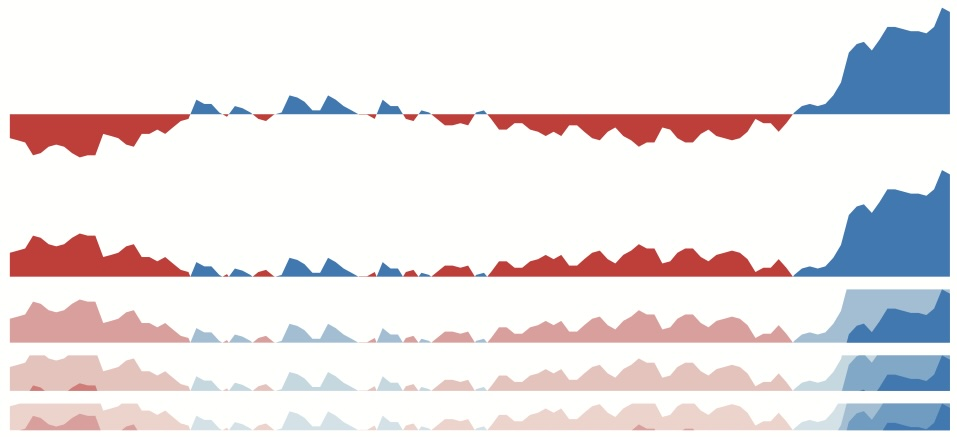
\includegraphics[width=.95\linewidth]{figs/100-horizon-graph.jpg}
\caption{Horizontni graf prikazuje časovno vrsto brezposelnosti skozi čas. Pozitivne in negativne vrednosti so prikazane z različnimi barvami, vrednosti pa so razdeljene v več pasov, ki se prekrivajo. Slika prikazuje tudi postopno transformacijo vizualizacije: od običajnega površinskega grafa, prek zrcaljenja negativnih vrednosti nad osnovno os, do razdelitve podatkov v več nivojev, ki so nato zloženi drug čez drugega. S tem se bistveno poveča gostota prikazanih podatkov, saj lahko enako časovno ločljivost prikažemo na precej manjši površini. Povzeto po Heer in sod. (2010).
\protect\label{fig:horizon}}
\end{figure}
%
Prednost horizontnih grafov je izjemna prostorska učinkovitost. V istem prostoru lahko prikažemo bistveno več podatkov kot s klasičnimi črtnimi diagrami. Slabost pa je nekoliko težje začetno razumevanje prikaza, saj mora opazovalec razumeti zlaganje pasov in pomen barvnih nivojev. Horizontni grafi zato niso najprimernejši za širše občinstvo, zelo uporabni pa so pri analitičnem delu strokovnjakov.

\vspace{1em}
\noindent {\bf Tokovni zemljevid.}
Tokovni zemljevid (angl. {\em flow map}) prikazuje gibanje količin skozi prostor. Takšne vizualizacije pogosto uporabljamo za prikaz migracij, trgovinskih tokov, transporta, širjenja bolezni ali zgodovinskih premikov vojska. Slika~\ref{fig:flow-map} prikazuje znameniti Minardov prikaz Napoleonovega pohoda na Moskvo. Vizualizacija velja za eno najboljših predstavitev podatkov vseh časov, saj v enem samem grafu združuje več različnih dimenzij podatkov. Debelina toka predstavlja velikost vojske, smer toka prikazuje gibanje, položaj predstavlja geografijo, dodatni graf pod zemljevidom pa prikazuje temperaturo med umikom vojske.
%
\begin{figure}[b]
\centering
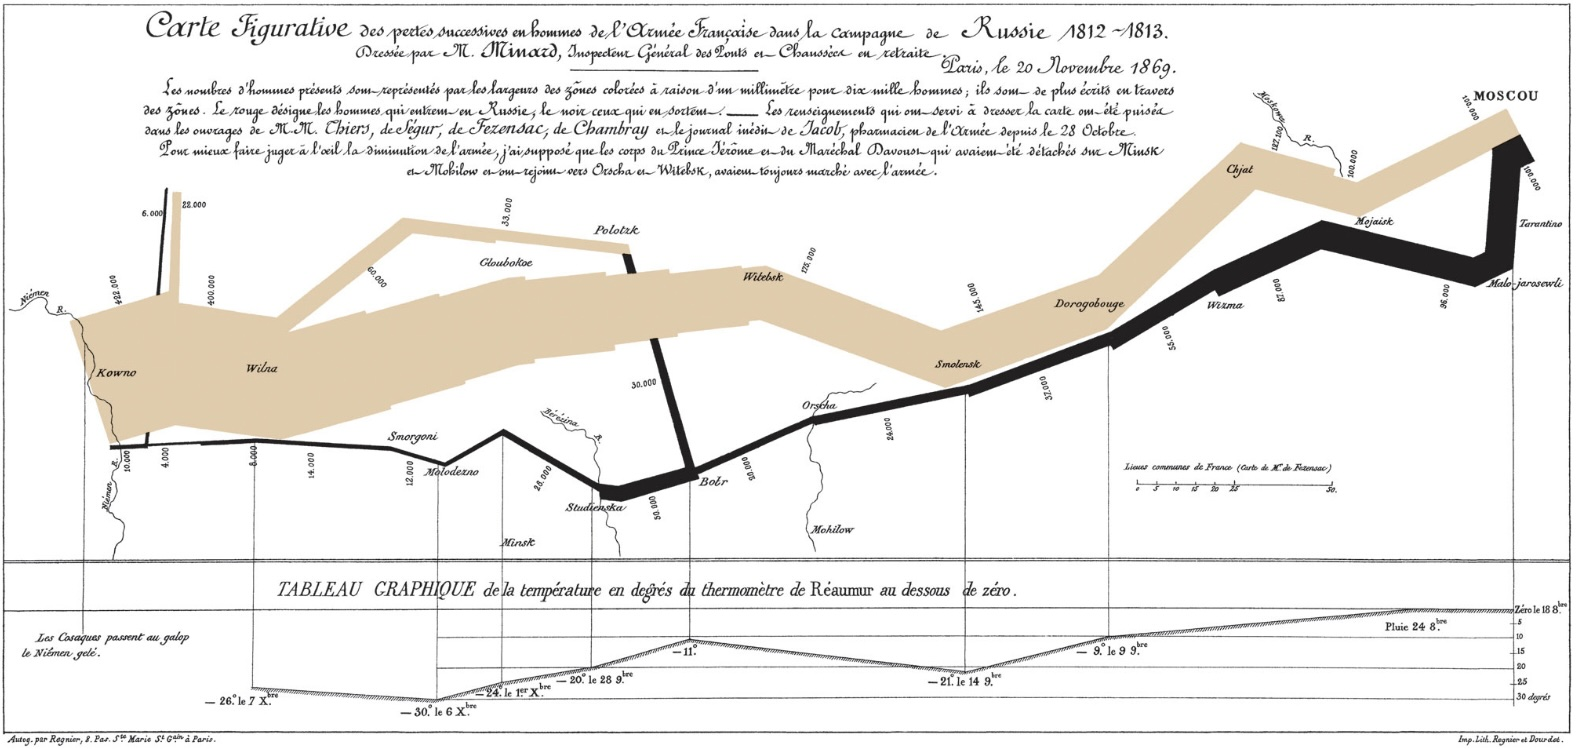
\includegraphics[width=.95\linewidth]{figs/100-flow-map.jpg}
\caption{Tokovni zemljevid Napoleonovega pohoda na Moskvo prikazuje gibanje vojske skozi prostor in čas. Debelina toka predstavlja velikost vojske, položaj označuje geografsko lokacijo, spodnji graf pa prikazuje temperaturo med umikom. Vizualizacija velja za eno najbolj znanih predstavitev večdimenzionalnih podatkov, ki jo je leta 1869 objavil francoski inženir Charles Joseph Minard v delu \emph{Carte figurative des pertes successives en hommes de l'Armée Française dans la campagne de Russie 1812--1813}.
\protect\label{fig:flow-map}}
\end{figure}
%
Tokovni zemljevidi so zanimivi predvsem zato, ker hkrati združujejo prostorske, časovne in količinske informacije. Dobro zasnovan tokovni zemljevid omogoča zelo intuitivno razumevanje kompleksnih procesov gibanja skozi prostor. Njihova slabost pa je možnost velike vizualne nepreglednosti pri večjem številu tokov, saj se poti hitro prekrivajo. Zato pogosto uporabljamo poenostavljanje poti, prosojnost ali interaktivno filtriranje.


\vspace{1em}
\noindent {\bf Drevesni zemljevid.}
Drevesni zemljevid (angl. {\em treemap}) je vizualizacija hierarhičnih podatkov, kjer so elementi predstavljeni z vgnezdenimi pravokotniki. Površina posameznega pravokotnika običajno predstavlja velikost ali pomembnost elementa, hierarhija pa je prikazana z vgnezdenostjo območij.
%
\begin{figure}[t]
\centering
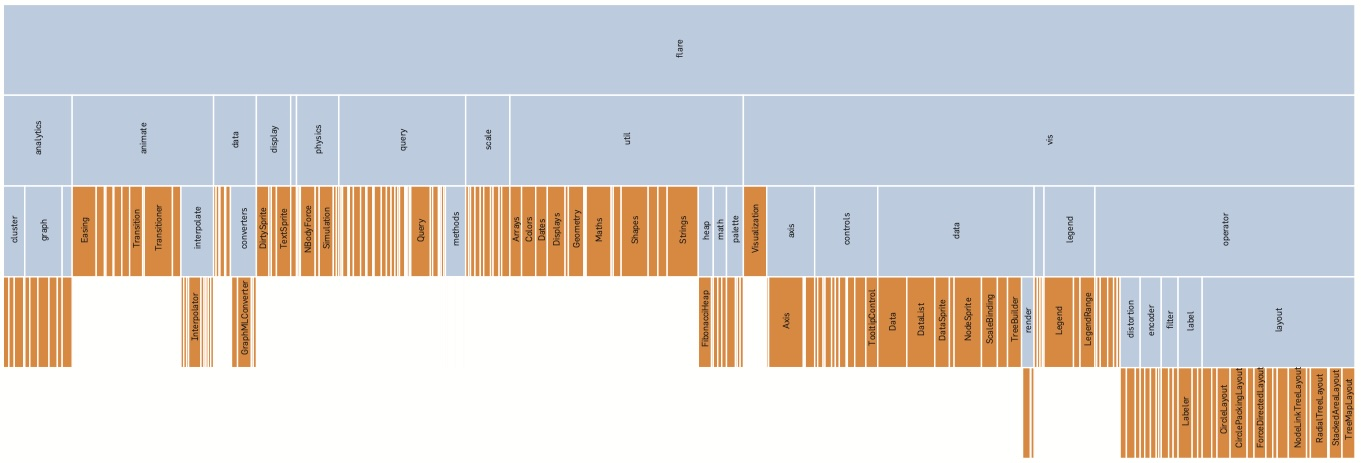
\includegraphics[width=.95\linewidth]{figs/100-treemap.jpg}
\caption{Drevesni zemljevid prikazuje hierarhijo programskih paketov. Posamezni pravokotniki predstavljajo razrede oziroma module, njihova površina pa velikost ali pomembnost posameznega elementa. Povzeto po Heer, Bostock in Ogievetsky, Figure~4f.
\protect\label{fig:treemap}}
\end{figure}
%
Na sliki~\ref{fig:treemap} je prikazan drevesni zemljevid hierarhije programskih paketov. Večji pravokotniki predstavljajo večje oziroma pomembnejše dele sistema. Ker drevesni zemljevid učinkovito izkorišča prostor, lahko na relativno majhni površini prikažemo zelo velike hierarhične strukture. 

Drevesne vizualizacije pogosto uporabljamo za prikaz uporabe diskovnega prostora, strukture finančnih trgov, organizacije datotek ali hierarhičnih klasifikacij. Ti prikazi so posebej uporabni, kadar želimo hitro oceniti relativne velikosti posameznih delov sistema. Njihova prednost je zelo učinkovita izraba prostora in dobra podpora primerjanju velikosti, slabost pa je nekoliko težje sledenje globlji hierarhični strukturi, saj pri zelo velikem številu nivojev vgnezdenost postane nepregledna. Prav tako primerjanje zelo podolgovatih pravokotnikov ni vedno intuitivno.

\vspace{1em}
\noindent {\bf Sončni izsek.}
Sončni izsek (angl. {\em sunburst diagram}) je radialna različica prostorsko zapolnjujoče predstavitve hierarhij. Hierarhija je prikazana s koncentričnimi krožnimi pasovi, kjer notranji krogi predstavljajo višje nivoje hierarhije, zunanji pa nižje nivoje. Na sliki~\ref{fig:sunburst} je prikazan sončni izsek iste hierarhične strukture kot pri drevesnem zemljevidu. V primerjavi z drevesnim zemljevidom sončni izsek pogosto bolj jasno poudari globino hierarhije, saj se nivoji naravno širijo navzven iz središča.

Vizualizacije tega tipa so lahko estetsko zelo privlačne in pogosto uporabljene v interaktivnih sistemih za raziskovanje podatkov. Posebej primerne so za prikaz hierarhičnih struktur, kjer nas zanima predvsem organizacija podatkov in odnosi med nivoji hierarhije. Njihova slabost je nekoliko slabša natančnost pri primerjanju površin in kotov, posebej pri zunanjih segmentih diagrama. Pri zelo globokih hierarhijah postanejo zunanji deli hitro preozki za učinkovito prikazovanje oznak.
%
\begin{marginfigure}
\centering
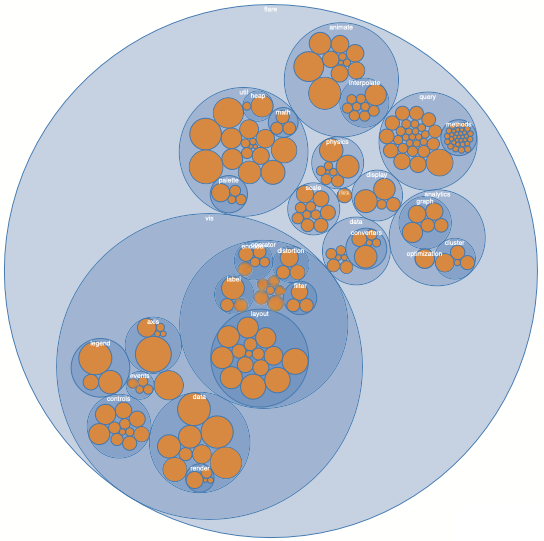
\includegraphics[width=1.0\linewidth]{figs/100-sunburst.png}
\caption{Sončni izsek prikazuje hierarhijo programskih paketov v radialni obliki. Notranji krogi predstavljajo višje nivoje hierarhije, zunanji pa podrobnejše podstrukture. Povzeto po Heer, Bostock in Ogievetsky, Figure~4e.
\protect\label{fig:sunburst}}
\end{marginfigure}
%

\vspace{1em}
\noindent {\bf Vizualizacija omrežij s silami.}
Veliko podatkovnih struktur lahko predstavimo kot omrežje povezav med objekti. Primeri vključujejo socialna omrežja, povezave med spletnimi stranmi, citatne mreže znanstvenih člankov ali biološke interakcije med proteini. Eden najpogostejših pristopov za prikaz takšnih podatkov so razporeditve na osnovi sil (angl. {\em force-directed layouts}).
%
\begin{figure}[t]
\centering
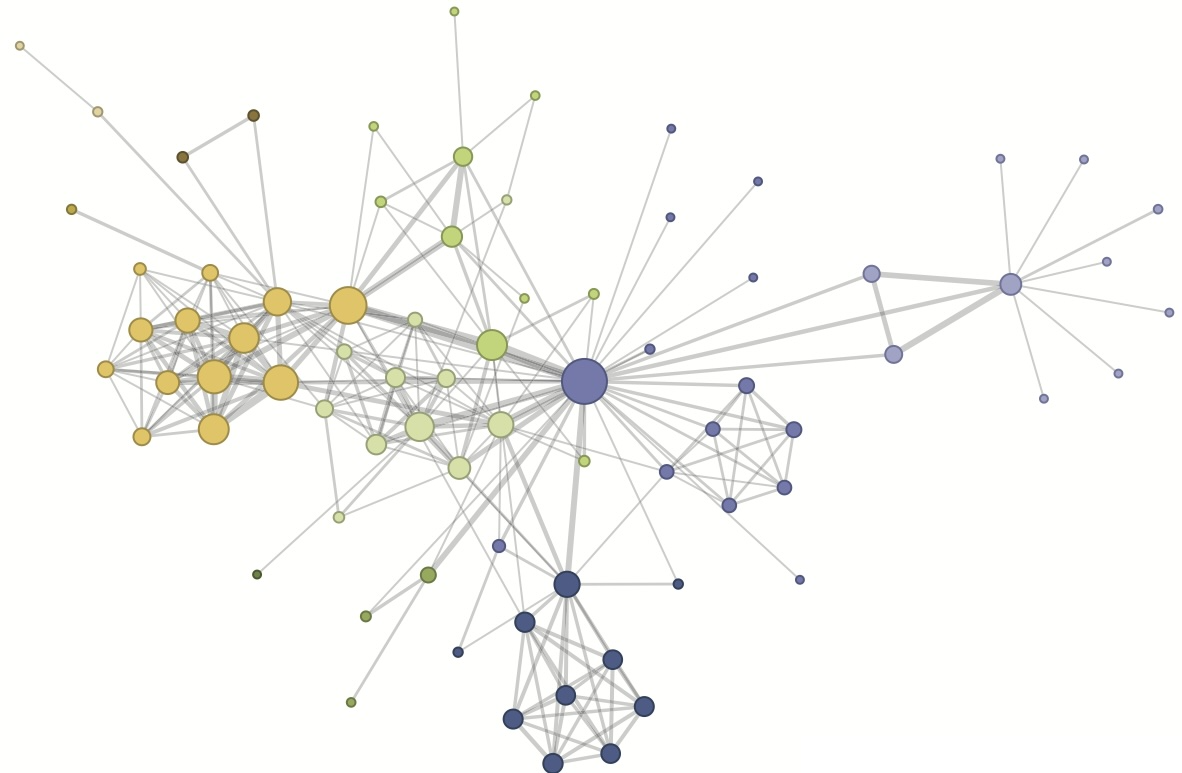
\includegraphics[width=.9\linewidth]{figs/100-force-layout.png}
\caption{Vizualizacija omrežja z razporeditvijo na osnovi sil. Vozlišča predstavljajo literarne like, povezave pa njihove skupne pojavitve v poglavjih romana. Položaj vozlišč je določen s simulacijo privlačnih in odbojnih sil. Povzeto po Heer, Bostock in Ogievetsky, Figure~5a.
\protect\label{fig:force-layout}}
\end{figure}
%
Na sliki~\ref{fig:force-layout} je prikazan primer omrežja likov iz romana \emph{Les Misérables}. Vozlišča predstavljajo posamezne like, povezave pa njihovo skupno pojavljanje v besedilu. Razporeditev vozlišč nastane s simulacijo fizikalnega sistema: povezani elementi se privlačijo, nepovezani pa odbijajo. Posledica je organska razporeditev, kjer se močno povezane skupine naravno združijo v gruče.  Vizualizacije tovrstnih grafov lahko omogočajo hitro prepoznavanje skupin, osrednjih vozlišč in mostov med različnimi deli omrežja. So med najpomembnejšimi pristopi pri analizi socialnih omrežij in kompleksnih grafov. Njihova glavna težava je uporaba na velikih podatkih. Pri zelo velikih omrežjih postanejo povezave nepregledne in vizualizacija se spremeni v tako imenovani klobčič povezav (angl. {\em hairball}), kjer posameznih struktur ni več mogoče razločiti. Zato pri večjih omrežjih pogosto uporabljamo filtriranje, združevanje vozlišč ali alternativne matrične predstavitve omrežij.

Pri sodobni podatkovni analizi pogosto uporabljamo tudi kompleksnejše vizualizacijske pristope. Njihov cilj ni zgolj estetska predstavitev podatkov, ampak učinkovito razkrivanje struktur, odnosov in vzorcev, ki jih z osnovnimi grafi težko opazimo. Pri njihovi uporabi pa moramo biti posebej pozorni na ravnotežje med informativnostjo in razumljivostjo. Če v isti prikaz vključimo preveč informacij, lahko vizualizacija hitro postane nepregledna. Zato je pri načrtovanju kompleksnih vizualizacij še posebej pomembno razumevanje podatkov, naloge analize in omejitev človekovega zaznavanja.



%%%%%%%%%%%%%%%

\section{Načela učinkovitega vizualnega oblikovanja}

Dobra vizualizacija mora opazovalcu omogočiti hitro, pravilno in čim manj naporno razumevanje podatkov. Zato pri načrtovanju grafov ni pomembna le izbira tipa vizualizacije, ampak tudi način uporabe barv, organizacija informacij, poudarjanje ključnih podatkov in odstranjevanje nepomembnih elementov.
%
\marginnote{Nekateri primeri v tem razdelku so povzeti po članku Jonathana Schwabisha \emph{The Practice of Visual Data Communication: What Works} iz revije \emph{Psychological Science in the Public Interest} (2021), ki na praktičnih primerih prikazuje vpliv oblikovnih odločitev na učinkovitost vizualizacij.}
%
Raziskave na področju vizualne percepcije kažejo, da lahko že majhne oblikovne odločitve močno vplivajo na interpretacijo podatkov. Vizualizacija mora zato podpirati človekove zaznavne sposobnosti in zmanjševati kognitivno obremenitev opazovalca. Cilj ni ustvarjanje vizualno spektakularnih grafov, ampak jasna in učinkovita komunikacija podatkov.

\vspace{1em}
\noindent {\bf Preprostost in jasnost.}
%
\begin{figure}[tb]
\centering
% Figure 1 iz Schwabish (2021): redesign slabega stolpčnega diagrama
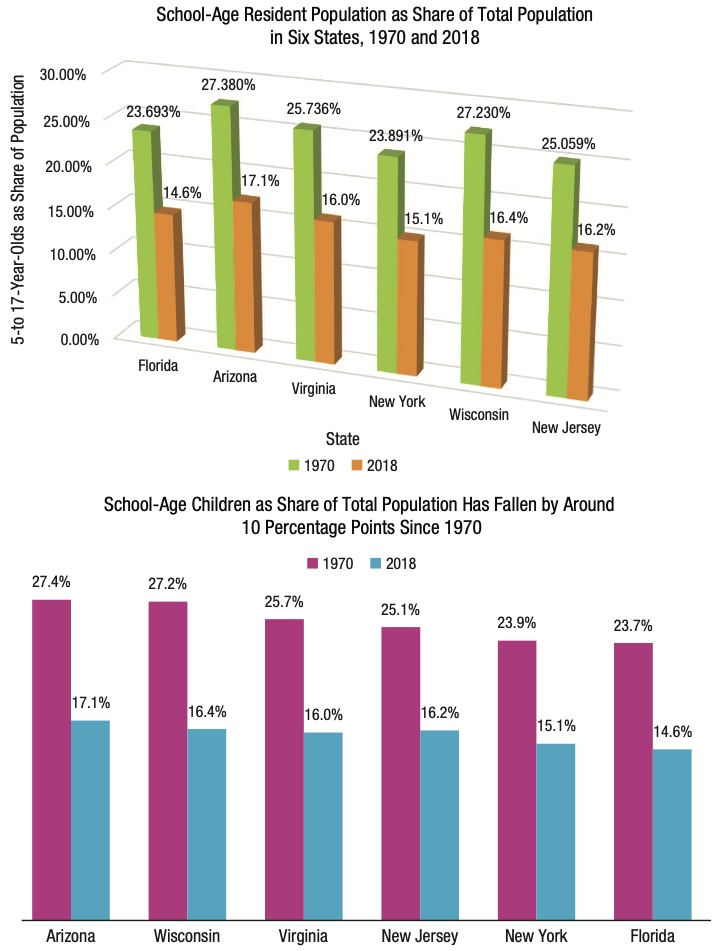
\includegraphics[width=.8\linewidth]{figs/100-barchart-redesign.jpg}
\caption{Primer izboljšanja stolpčnega diagrama. Zgornji graf uporablja tridimenzionalni prikaz, močne mreže in nepregledne oznake, spodnji pa enostavnejšo postavitev, neposredno označevanje podatkov in bolj pregledno uporabo barv. Povzeto po Schwabish (2021). Odstranitev nepotrebnih grafičnih elementov bistveno izboljša preglednost in usmeri pozornost na podatke namesto na dekoracijo. Takšni odvečni elementi so pogosto označeni z izrazom \emph{chartjunk}, ki opisuje grafične dodatke brez analitične vrednosti.
\protect\label{fig:design-bar-redesign}}
\end{figure}
%
Graf naj vsebuje le elemente, ki prispevajo k razumevanju podatkov. Nepotrebni dekorativni učinki, tridimenzionalni prikazi, ogromna omrežja ali pretirano število oznak pogosto zmanjšajo preglednost in otežijo interpretacijo. Glavno sporočilo vizualizacije mora biti razvidno takoj. Opazovalec ne bi smel ugibati, kaj graf prikazuje ali kateri podatki so pomembni. Ključne informacije morajo biti vizualno poudarjene, manj pomembni elementi pa umaknjeni v ozadje.

\vspace{1em}
\noindent {\bf Vizualna hierarhija in usmerjanje pozornosti.}
Dobra vizualizacija mora opazovalca usmerjati k najpomembnejšim informacijam. Vizualna hierarhija določa, katere elemente zaznamo najprej in katere kasneje. To dosežemo z uporabo kontrasta, velikosti, debeline črt, položaja ali barve. Pogosto želimo poudariti le manjši del podatkov, medtem ko preostale informacije ostanejo v ozadju. Zato številni sodobni grafi uporabljajo nevtralne sive tone za večino elementov, ključne podatke pa poudarijo z izrazitejšo barvo. Tak pristop zmanjša vizualni šum in omogoči hitrejše razumevanje bistvenih informacij. Vizualna hierarhija je posebej pomembna pri kompleksnih grafih, kjer bi enakovredno poudarjanje vseh elementov povzročilo nepreglednost in povečalo kognitivno obremenitev opazovalca.
%
\begin{figure}[htb]
\centering
% Figure 6 iz Schwabish (2021): uporaba dot plota in vizualne hierarhije
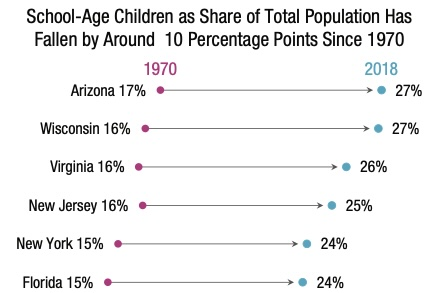
\includegraphics[width=.6\linewidth]{figs/100-design-dotplot.jpg}
\caption{Točkovni prikaz uporablja nevtralne elemente in poudarjene oznake za usmerjanje pozornosti opazovalca na ključne razlike med podatki. Neposredno označevanje podatkov zmanjšuje potrebo po ločenih legendah in izboljša preglednost vizualizacije. Povzeto po Schwabish (2021).
\protect\label{fig:design-dotplot-highlight}}
\end{figure}
%

\vspace{1em}
\noindent {\bf Doslednost in zmanjševanje kognitivne obremenitve.}
Vizualizacije morajo uporabljati dosledne grafične konvencije. Enake barve naj predstavljajo iste kategorije, osi naj uporabljajo enake merske enote, tipografija in oznake pa naj bodo poenotene skozi celotno predstavitev. 

Nedoslednosti povečajo kognitivno obremenitev, saj mora opazovalec ponovno interpretirati pomen posameznih elementov. Vizualizacija mora biti zasnovana tako, da opazovalec čim manj časa porabi za razumevanje same strukture grafa in čim več za interpretacijo podatkov. Kognitivno obremenitev zmanjšujemo tudi z neposrednim označevanjem podatkov namesto ločenih legend, z uporabo kratkih in informativnih naslovov ter z logično razporeditvijo elementov. Posebej učinkovite so vizualizacije, kjer so besedilo, oznake in grafični elementi tesno povezani.

%
\begin{figure}[htb]
\centering
% kombinacija Figure 5 in Figure 6 iz Schwabish (2021): bar chart vs dot plot
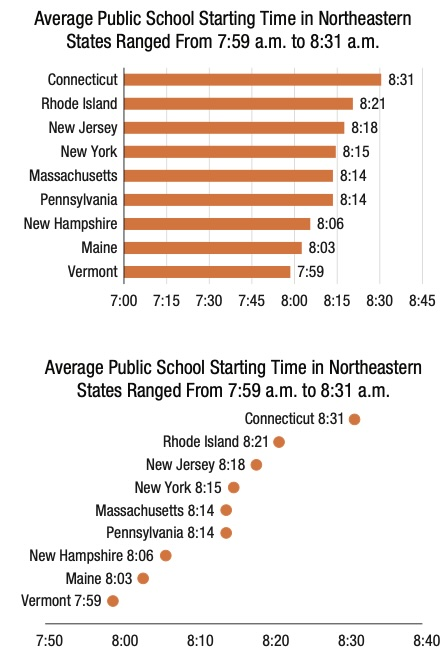
\includegraphics[width=.3\linewidth]{figs/100-design-bar-dotplot.jpg}
\caption{Primerjava stolpčnega diagrama in točkovnega prikaza. Točkovni prikaz uporablja manj vizualnega prostora in omogoča hitrejše primerjanje vrednosti ter sprememb med kategorijami. Povzeto po Schwabish (2021).
\protect\label{fig:design-dotplot}}
\end{figure}
%

\vspace{1em}
\noindent {\bf Barve in dostopnost.}
Barva je eden najmočnejših vizualnih elementov, vendar jo moramo uporabljati previdno. Primerna je predvsem za razlikovanje kategorij, poudarjanje pomembnih podatkov in prikaz intenzitete vrednosti. Pomemben delež populacije ima različne oblike motenj barvnega zaznavanja, najpogosteje težave pri razlikovanju rdeče in zelene barve. Vizualizacije morajo zato ostati razumljive tudi uporabnikom z barvno slepoto ter pri sivinskem prikazu. Zato se pogosto izogibamo problematičnim kombinacijam ter uporabljamo perceptualno primerne barvne lestvice.

\vspace{1em}
\noindent {\bf Oblikovne odločitve vplivajo na interpretacijo.}
Na interpretacijo podatkov močno vpliva tudi način njihove vizualne predstavitve. Že majhne oblikovne odločitve lahko močno vplivajo na interpretacijo in ustvarijo napačen vtis o trendih ali razlikah med podatki. Posebej problematične so neustrezne osi, pretirano poudarjeni elementi ali neprimerna uporaba linij in površin. Takšne odločitve lahko povzročijo, da opazovalec zazna trend ali povezavo, ki v podatkih dejansko ne obstaja.
%
\begin{figure}[htb]
\centering
% Figure 3 iz Schwabish (2021): primer zavajajoče uporabe obrnjene osi
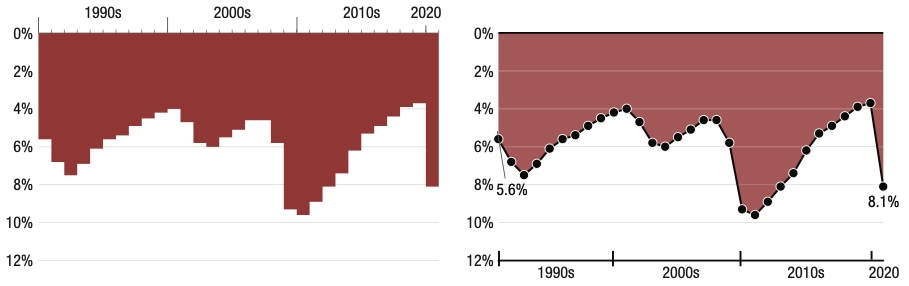
\includegraphics[width=.95\linewidth]{figs/100-design-axis-example.jpg}
\caption{Dve vizualizaciji istih podatkov z obrnjeno navpično osjo. Leva različica uporablja stolpce in pravilno poudarja dolžino kot nosilko informacije, desna pa zaradi linije in položaja točk ustvarja zavajajoč vtis trenda. Povzeto po Schwabish (2021).
\protect\label{fig:design-axis-example}}
\end{figure}
%


Učinkovita vizualizacija zato zahteva več kot zgolj tehnično znanje izdelave grafov. Zahteva razumevanje človekove percepcije, načel grafične komunikacije ter prilagoditev ciljnemu občinstvu. Dobra vizualizacija opazovalcu olajša razumevanje podatkov in odnosov med njimi.

%%%%

\section{Zavajajoče vizualizacije}

Vizualizacije podatkov imajo velik vpliv na razumevanje informacij, zato lahko že majhne oblikovne odločitve bistveno spremenijo interpretacijo podatkov.
%
\marginnote{Nekateri primeri v tem razdelku so povzeti po članku \emph{The Science of Visual Data Communication: What Works} (Franconeri idr., 2021), ki vključuje tudi primere napak in zavajajoče načine prikaza podatkov.}
%
Grafi pogosto delujejo objektivno in znanstveno, vendar lahko z neustreznim oblikovanjem ustvarijo zavajajoč vtis o velikosti razlik, trendih ali povezavah med spremenljivkami. Zaradi tega je etično oblikovanje vizualizacij pomemben del odgovorne komunikacije podatkov.

\vspace{1em}
\noindent {\bf Prirezane osi in popačene skale.}
Eden najpogostejših načinov zavajanja je uporaba prirezanih osi. Če navpična os ne začne pri nič, lahko že majhne razlike med vrednostmi delujejo bistveno večje, kot so v resnici. Takšne manipulacije pogosto pretirano poudarijo trende ali razlike med skupinami. Podoben učinek imajo popačene skale, kjer razmiki med vrednostmi niso linearni ali pa so vizualno predstavljeni nesorazmerno glede na dejanske podatke. Opazovalec običajno zazna predvsem vizualno velikost razlik in manj pogosto natančno preverja numerične vrednosti na osi. Takšni prijemi so pogosti v medijih, politiki in poslovnih predstavitvah, kjer želimo določene razlike poudariti bolj, kot to upravičujejo podatki.
%
\begin{figure}[t]
\centering
% Figure 3 iz Franconeri et al. (2021): zavajajoče osi in raztegovanje skale
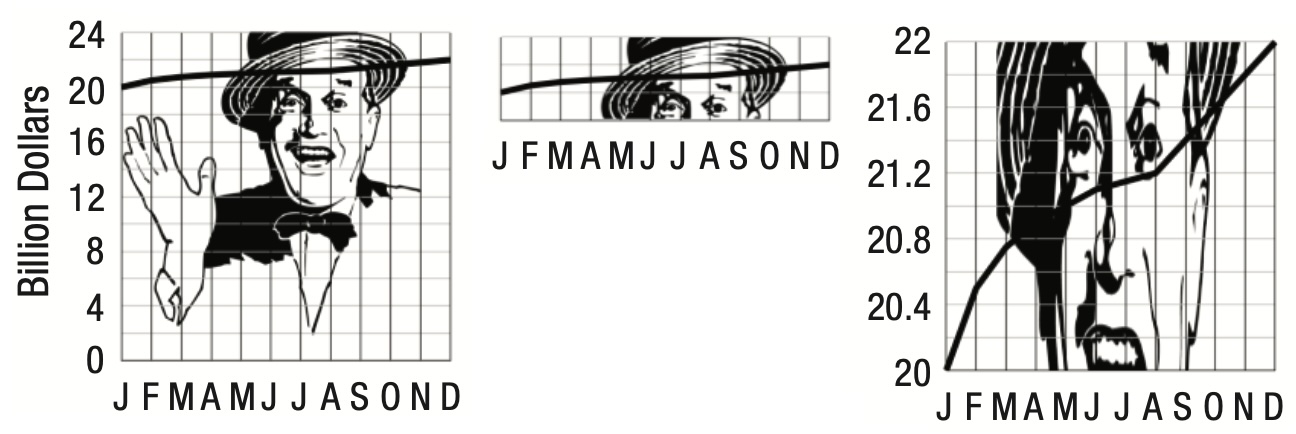
\includegraphics[width=.95\linewidth]{figs/100-err-truncated-axis.jpg}
\caption{Primer vpliva prirezanih osi in raztegnjenih skal na interpretacijo podatkov. Enaki podatki lahko zaradi drugačne izbire osi ustvarijo bistveno drugačen vtis o velikosti razlik ali trendov. Povzeto po Franconeri in sod. (2021).
\protect\label{fig:ethics-truncated-axis}}
\end{figure}
%

\vspace{1em}
\noindent {\bf Zavajajoče barvne lestvice.}
Barva močno vpliva na zaznavanje intenzitete podatkov. Neprimerne barvne lestvice lahko ustvarijo umetne meje med vrednostmi ali poudarijo razlike, ki v podatkih niso pomembne. Posebej problematične so lestvice z močnimi prehodi med različnimi barvnimi kategorijami, na primer med modro, zeleno in rdečo. Človek zazna prehod med barvnimi kategorijami kot večjo razliko, kot dejansko obstaja v podatkih. Zaradi tega lahko kontinuirani podatki delujejo bolj diskretno ali dramatično. Pri oblikovanju vizualizacij zato uporabljamo perceptualno enakomerne barvne lestvice, kjer sprememba barve čim bolj ustreza dejanski spremembi podatkovnih vrednosti.

\vspace{1em}
\noindent {\bf Prekrivanje podatkov in izbira prikazanih primerov.}
Pri velikih množicah podatkov lahko pride do prekrivanja točk (\emph{overplotting}), kjer posamezne vrednosti zakrijejo druge. Posledično lahko pomembni vzorci ostanejo skriti ali pa vizualizacija daje napačen vtis gostote podatkov. Zavajajoč učinek lahko povzroči tudi selektivna izbira podatkov (angl. \emph{cherry-picking}), kjer avtor prikaže le tiste podatke, ki podpirajo želeni zaključek. Vizualizacija lahko tako deluje prepričljivo, čeprav ne predstavlja celotne slike. Zato morajo vizualizacije jasno prikazati obseg podatkov, uporabljene filtre in morebitne omejitve pri izbiri vzorca.

\vspace{1em}
\noindent {\bf Korelacija ni vzročnost.}
Vizualizacije pogosto učinkovito pokažejo povezave med spremenljivkami, vendar povezava sama po sebi še ne pomeni vzročne zveze. Dve spremenljivki sta lahko močno povezani, čeprav med njima ni neposrednega vpliva. Razsevni in linijski diagrami lahko hitro ustvarijo vtis vzročne povezave, posebej kadar sta podatka prikazana skupaj skozi čas. Opazovalci pogosto intuitivno sklepajo, da ena spremenljivka povzroča drugo, čeprav je povezava lahko posledica tretjega dejavnika ali naključja. Slika~\ref{fig:ethics-patterns} prikazuje, kako hitro opazimo vzorce in strukture v podatkih, tudi kadar ti niso nujno analitično pomembni. Pri interpretaciji vizualizacij moramo zato ločiti med opisom podatkov in dejanskimi vzročnimi razlagami.
%
\begin{marginfigure}
\centering
% Figure 7 iz Franconeri et al. (2021): omejitve vizualnega primerjanja in zaznavanja vzorcev
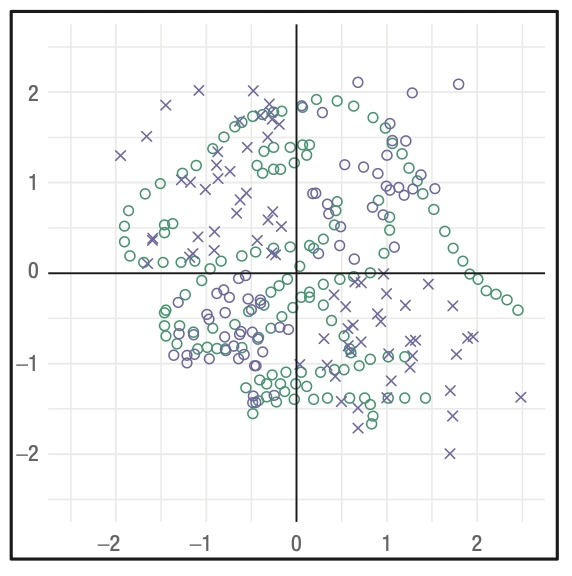
\includegraphics[width=.9\linewidth]{figs/100-err-patterns.jpg}
\caption{Človekov vizualni sistem hitro zaznava vzorce in povezave med podatki, vendar lahko to vodi tudi do napačnega sklepanja o odnosih med spremenljivkami. Povzeto po Franconeri idr. (2021).
\protect\label{fig:ethics-patterns}}
\end{marginfigure}
%

\vspace{1em}
\noindent {\bf Prikazovanje negotovosti.}
Podatki pogosto vsebujejo negotovost, ki jo moramo ustrezno prikazati. Če negotovosti ne pokažemo, lahko vizualizacija daje lažen vtis natančnosti in gotovosti. Negotovost običajno prikazujemo z intervali zaupanja, območji verjetnosti, razponi napak ali več možnimi scenariji. Posebej pomembno je to pri vremenskih napovedih, epidemioloških modelih, ekonomskih napovedih in znanstvenih rezultatih. Vizualizacija mora zato jasno pokazati:
\begin{itemize}
\item katere podatke prikazujemo,
\item kakšna je stopnja negotovosti,
\item katere omejitve imajo podatki,
\item in katerih zaključkov iz vizualizacije ne moremo zanesljivo sklepati.
\end{itemize}

%%%%%%

\section{Primeri izbire in izboljšanja vizualnih predstavitev}

Iste podatke lahko prikažemo na več načinov, pri čemer vsak način poudari nekoliko drug vidik: prostorski vzorec, primerjavo med enotami, povezavo med spremenljivkami, natančne vrednosti ali bolj intuitivno razumevanje časovnih podatkov. V nadaljevanju si ogledamo nekaj primerov iz članka Schwabisha (2021) v reviji {\em Psychological Science in the Public Interest}, ki pokažejo, kako lahko že razmeroma preproste spremembe izboljšajo razumljivost in uporabnost vizualizacije. Avtor pri tem uporablja podatke o začetku pouka v javnih šolah v ZDA ter pokaže, da lahko tudi z običajnimi orodji pripravimo precej različne, a učinkovite predstavitve podatkov.

\vspace{1em}
\noindent {\bf Prostorski podatki.}
Pri prostorskih podatkih pogosto najprej pomislimo na običajen zemljevid, vendar ta ni vedno najboljša izbira. Klasični koropletni zemljevid dobro ohranja geografsko obliko držav in zato hitro razkrije prostorske vzorce, na primer da se pouk v južnih zveznih državah začne nekoliko prej. Po drugi strani velikost geografskih območij vpliva na zaznano pomembnost podatkov: velike države na zemljevidu zavzamejo več prostora, čeprav nimajo nujno večje analitične teže. Mrežni zemljevid s ploščicami ta problem zmanjša, saj vsaki državi nameni enako velik prostor, hkrati pa omogoča dodajanje oznak ali majhnih grafičnih elementov znotraj vsake celice (slika~\ref{fig:schwabish-maps}). Tak prikaz žrtvuje nekaj geografske natančnosti, vendar lahko izboljša primerljivost in poveča uporabnost prikaza za bralca.

\begin{figure}[t]
\centering
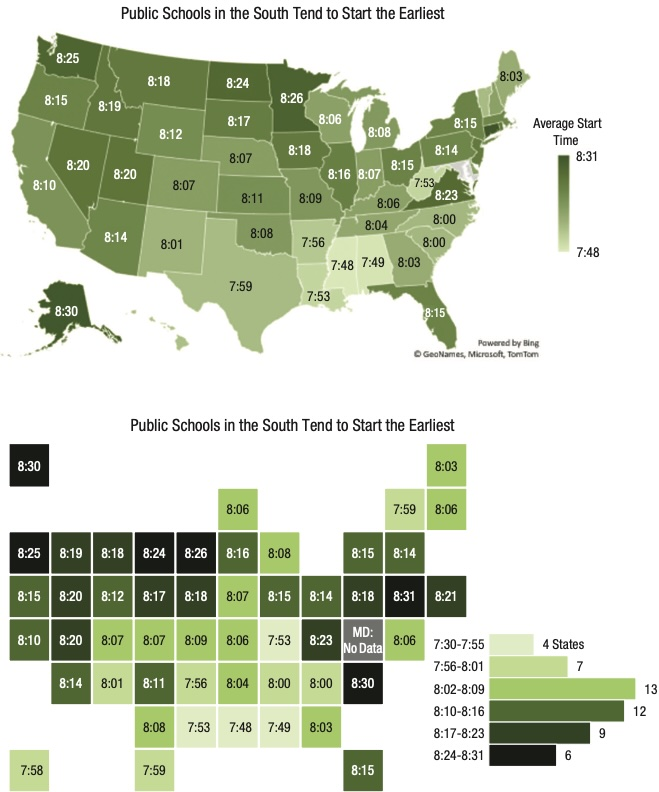
\includegraphics[width=.95\linewidth]{figs/100-schwa-maps.jpg}
\caption{Dva načina prikaza prostorskih podatkov o povprečnem začetku pouka v javnih šolah v ZDA: običajni koropletni zemljevid in mrežni zemljevid s ploščicami. Prvi bolje ohranja geografsko obliko, drugi pa vsaki državi nameni enak prostor in tako olajša primerjavo med državami.
\protect\label{fig:schwabish-maps}}
\end{figure}

\vspace{1em}
\noindent {\bf Stolpci ali točke.}
Stolpčni diagram je ena najbolj znanih in razumljivih vizualizacij za primerjanje vrednosti med skupinami. Njegova prednost je, da dolžine stolpcev primerjamo razmeroma natančno, še posebej, kadar imajo skupno izhodišče. Toda stolpčni diagrami lahko postanejo vizualno težki, posebej pri večjem številu kategorij ali daljših oznakah. Točkovni diagram za iste podatke pogosto uporablja manj grafičnega prostora in pusti več prostora za oznake, komentarje ali neposredno označevanje vrednosti (slika~\ref{fig:schwabish-bars-dots}). Primer zato ne kaže, da je stolpčni diagram napačen, ampak da lahko preprostejša in lažja grafična oblika bolj berljiva, kadar nas zanima predvsem vrstni red in primerjava posameznih vrednosti.

\begin{figure}[t]
\centering
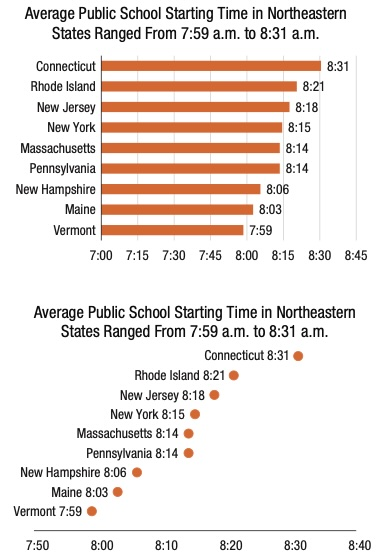
\includegraphics[width=.75\linewidth]{figs/100-schwa-bars-dots.jpg}
\caption{Primerjava stolpčnega diagrama in točkovnega prikaza za iste podatke. Stolpci omogočajo neposredno primerjavo dolžin, točkovni prikaz pa zmanjša vizualno težo grafa in omogoči preglednejše označevanje vrednosti.
\protect\label{fig:schwabish-bars-dots}}
\end{figure}

\vspace{1em}
\noindent {\bf Razsevni diagram kot prostor za razlago.}
Razsevni diagram je osnovni prikaz za raziskovanje povezave med dvema numeričnima spremenljivkama. Vendar dober razsevni diagram ni le oblak točk. Z dodatnimi oznakami, povprečnimi črtami, pojasnili osi in označenimi osamelci lahko bralcu pomagamo razumeti, kaj naj v grafu opazi. Pri podatkih o začetku pouka in deležu šoloobveznih otrok v populaciji lahko vodoravne in navpične referenčne črte razdelijo prostor grafa na območja nad in pod povprečjem, oznake izbranih držav pa usmerijo pozornost na primere, ki posebej odstopajo (slika~\ref{fig:schwabish-scatter}). Pri takem prikazu je pomembno ravnotežje: preveč oznak graf obremeni, premišljene oznake pa lahko bistveno izboljšajo interpretacijo.

\begin{figure}[t]
\centering
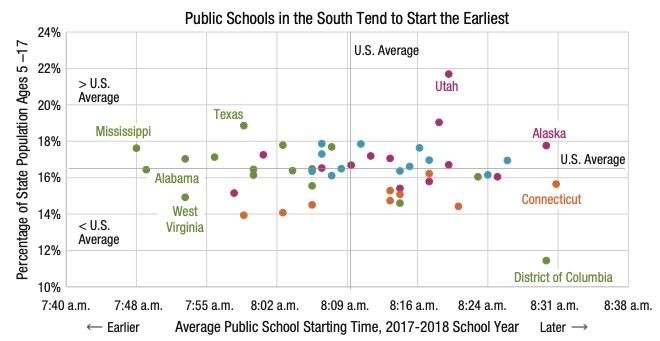
\includegraphics[width=.95\linewidth]{figs/100-schwa-scatter.jpg}
\caption{Razsevni diagram povezave med povprečnim začetkom pouka in deležem prebivalstva v starosti od 5 do 17 let. Referenčne črte, oznake osi in izbrane oznake držav pomagajo bralcu razumeti strukturo podatkov ter prepoznati osamelce.
\protect\label{fig:schwabish-scatter}}
\end{figure}

\vspace{1em}
\noindent {\bf Tudi tabela je vizualizacija.}
Tabele pogosto razumemo kot nasprotje grafov, vendar so tudi tabele oblika vizualne predstavitve podatkov. Slabo oblikovana tabela oteži primerjanje vrednosti: glave stolpcev niso jasno ločene, besedilo in številke niso ustrezno poravnani, število decimalnih mest je nedosledno, enote pa so zapisane neenotno. Z razmeroma majhnimi popravki lahko tabela postane bistveno preglednejša: glave stolpcev so jasno ločene, besedilo je levo poravnano, številke desno poravnane, natančnost zapisa je poenotena, dodani majhni stolpci v zadnjem stolpcu pa pomagajo hitro zaznati vzorec (slika~\ref{fig:schwabish-table}). Tak primer je posebej pomemben za poročila in znanstvena besedila, kjer tabele pogosto nosijo veliko informacij.

\begin{figure}[t]
\centering
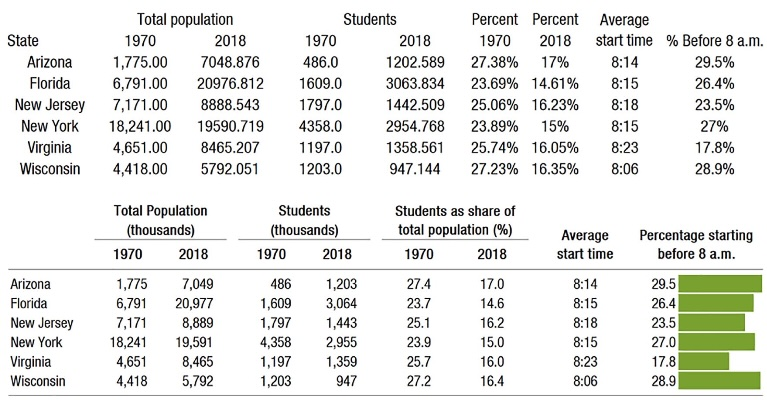
\includegraphics[width=.95\linewidth]{figs/100-schwa-table.jpg}
\caption{Primer izboljšanja tabele. Preglednejša različica uporablja jasnejšo hierarhijo glave, ustrezno poravnavo besedila in številk, enotno število decimalnih mest ter majhne stolpčne prikaze za hitrejše zaznavanje vzorcev. Povzeto po Schwabish (2021), Figure~10.
\protect\label{fig:schwabish-table}}
\end{figure}

\vspace{1em}
\noindent {\bf Vizualizacija, ki izhaja iz pomena podatkov.}
Kadar podatki opisujejo čas dneva, lahko vizualizacija izkoristi obliko, ki je bralcu že znana iz vsakdanjega življenja. Namesto zemljevida, stolpčnega grafa ali tabele lahko začetke pouka razporedimo po številčnici ure, kjer položaj oznake neposredno ustreza času začetka (slika~\ref{fig:schwabish-clock}). Tak prikaz ni nujno najbolj standarden, vendar je dobro usklajen s pomenom podatkov: bralec takoj razume, da gre za čas, in lahko poišče posamezno državo na znani krožni strukturi. Primer kaže, da je lahko nekoliko bolj igriva ali nestandardna vizualizacija še vedno analitično smiselna, če podpira razumevanje podatkov in ne zakriva njihovega pomena.

\begin{figure}[t]
\centering
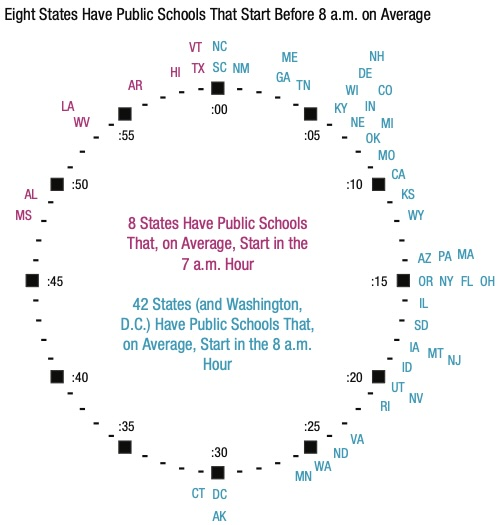
\includegraphics[width=.7\linewidth]{figs/100-schwa-clock.jpg}
\caption{Alternativni prikaz časovnih podatkov s številčnico ure. Oznake držav so razporejene glede na povprečni čas začetka pouka, barva pa dodatno loči države, kjer se pouk v povprečju začne pred osmo uro.
\protect\label{fig:schwabish-clock}}
\end{figure}

Skupno sporočilo teh primerov je, da učinkovita vizualizacija nastane iz povezave med podatki, nalogo in občinstvom. Ni dovolj, da izberemo prvi graf, ki ga ponudi programsko orodje. Premisliti moramo, kaj želimo poudariti, katere primerjave naj bralec opravi, koliko razlage potrebuje in kateri prikaz bo podatke predstavil najbolj jasno. Včasih je to običajen stolpčni diagram, drugič zemljevid, tabela, točkovni prikaz ali celo ura.

%%%%%%
\section{Vizualna analitika in interaktivnost}

Sodobna vizualizacija podatkov ni več omejena le na statične slike v tiskanih medijih (članki, poročila) ali na drsnicah. Vedno pomembnejšo vlogo imajo interaktivne vizualizacije, pri katerih lahko uporabnik podatke raziskuje, spreminja pogled na podatke in se osredotoča na zanimive podmnožice podatkov. Tak pristop uporabljajo tehnike \emph{vizualne analitike}, ki združujejo vizualizacijo, interakcijo in analitično raziskovanje podatkov.

Ko uporablja vizualne vmesnike, uporabnik ni le pasivni opazovalec grafične predstavitve, ampak lahko aktivno spreminja prikaz podatkov in, kolikor mnu vmesnik dopušča, preiskuje in raziskuje podatke. Najpogostejše interakcije, ki jih taki sistemi implementirajo, vključujejo:
\begin{itemize}
    \item \textbf{filtriranje}, kjer izberemo le del podatkov,
    \item \textbf{brushing}, kjer označimo podmnožico podatkov v enem prikazu,
    \item \textbf{povečevanje in premikanje} (\emph{zooming} in \emph{panning}), kjer se lahko osredotočimo na del podatkov,
    \item \textbf{izbiro elementov} (\emph{selection}), kjer v eni vizualizaciji izberemo elemente, ki jih potem navadno prikažemo na dodatni vizualizaciji,
    \item \textbf{podrobnosti na zahtevo} (\emph{details on demand}), kjer se dodatne informacije prikažejo ob kliku miške ali ko stojimo z miško na določenem elementu, za katerega nas zanimjo dodatne podrobnosti, in
    \item \textbf{barvanje in označevanje skupin}, kjer na grafični način uporabnik razdeli podatke v njemu zanimive skupine, za katere je potem seveda potrebno prikazati razlike z dodatnimi prikazi ali v dodatnih vizualizacijah.
\end{itemize}

V preiskovalne namene so posebej uporabne povezane vizualizacije (\emph{linked visualizations}). Pri takem pristopu izbira podatkov v enem grafu (avtomatičo in hipno) vpliva tudi na druge prikaze. Če na primer v razsevnem diagramu označimo določeno skupino podatkov, se isti podatki istočasno označijo tudi v histogramu ali tabeli. Tak način omogoča učinkovito raziskovanje večdimenzionalnih podatkov in hitro odkrivanje povezav med atributi.

Interaktivne vizualizacije pogosto združujemo v nadzorne plošče oziroma \emph{dashboards}. Ti prikazi vsebujejo več med seboj povezanih grafov, filtrov in tabel, ki uporabniku omogočajo pregled nad podatki in interaktivno analizo. Podoben pristop uporabljajo tudi sistemi za vizualno podatkovno analitiko, kot je ljubljanski Orange Data Mining, kjer uporabnik gradi analitični potek dela (\emph{workflow}) s povezovanjem posameznih komponent za uvoz podatkov, analizo, modeliranje in vizualizacijo in na ta način določi način obdelave podatkov ter med sabo poveže vizualizacije.

Podporo za interaktivno vizualizacijo danes ponujajo številna programska orodja. Tableau je eno najbolj razširjenih okolij za pripravo interaktivnih nadzornih plošč in raziskovalno analizo podatkov, saj omogoča hitro povezovanje grafov, filtrov in interaktivnih pogledov brez programiranja. Podobno vlogo ima Microsoft Power BI, ki je močno povezan z ekosistemom podatkovnih storitev podjetja Microsoft in se pogosto uporablja za poslovno analitiko ter spremljanje podatkov v realnem času. Orodja, kot je Orange Data Mining, KNIME in RapidMiner, pa so bolj usmerjena v raziskovalno analizo in strojno učenje, kjer uporabnik z vizualnim povezovanjem komponent gradi celoten analitični potek dela. Skupna značilnost teh sistemov je podpora interaktivnosti, povezanim vizualizacijam ter postopnemu raziskovanju podatkov.

Poseben izziv predstavljajo podatki v realnem času oziroma pretočni podatki (\emph{streaming data}). Pri takih podatkih se vizualizacija sproti posodablja, ko prihajajo novi podatki. Takšne prikaze srečamo pri spremljanju omrežnega prometa, finančnih trgov, senzorjev ali družbenih omrežij. Poleg samega prikaza podatkov je pri takih sistemih pomembna tudi hitrost osveževanja, poudarjanje pomembnih sprememb ter preprečevanje preobremenitve uporabnika z informacijami.

Interaktivnost zato ni le estetski dodatek, ampak pomembno orodje za raziskovanje podatkov. Dobro zasnovane interaktivne vizualizacije uporabniku omogočajo, da sam raziskuje podatke, postavlja vprašanja in postopoma gradi razumevanje analiziranega problema.


\section{Pripovedovanje zgodb s podatki}

Vizualizacija podatkov je predvsem način komunikacije o spoznanjih, ki smo jih na osnovi podatkov pridobili. Pri pripravi vizualizacije zato običajno pričnemo z vprašanjem, kaj želimo sporočiti. Isti podatki lahko podprejo različne zgodbe: lahko poudarimo trend, primerjavo, izjemen primer, negotovost ali spremembo skozi čas. Naloga avtorja vizualizacije je, da izbere prikaze ali redosled prikazov, ki podprejo glavno sporočilo, ter usmeri pozornost bralca na pomembne dele podatkov in vzorce. Pri tem imajo pomembno vlogo barva, kontrast, velikost elementov, označevanje in komentarji (\emph{annotation}), s katerimi lahko poudarimo ključne informacije in zmanjšamo vpliv manj pomembnih podrobnosti.

Učinkovita vizualizacija podatkov zato pogosto deluje kot pripoved (\emph{storytelling with data}). Bralca vodi skozi podatke, postopoma razkriva pomembne vzorce in pomaga pri interpretaciji rezultatov. Tak pristop je posebej značilen za novinarske in spletne interaktivne vizualizacije, kjer uporabnik podatke raziskuje korak za korakom. Pri tem moramo vedno upoštevati tudi občinstvo: vizualizacije za strokovnjake lahko vsebujejo več podrobnosti in kompleksnejše prikaze, medtem ko morajo biti vizualizacije za širšo javnost bolj neposredne in hitro razumljive. Dobra vizualizacija zato ne prikazuje le podatkov, ampak pomaga oblikovati razumevanje problema.


\section{Programska orodja za gradnjo vizualizacij}

Vizualizacije podatkov danes pogosto ne nastajajo več kot ročno narisane slike,
temveč kot rezultat programskega opisa podatkov, njihovih preslikav v vizualne
elemente in pravil interakcije. Tak pristop je posebej pomemben v podatkovni
znanosti, kjer želimo grafe graditi ponovljivo, jih prilagajati novim podatkom
in jih vključevati v poročila, spletne strani ali interaktivna analitična okolja.

Najpreprostejši primer takega pristopa v Pythonu je uporaba knjižnice
\texttt{matplotlib}. Ta omogoča natančen nadzor nad posameznimi elementi grafa
in je osnova številnih drugih vizualizacijskih knjižnic.

\vspace*{3mm}
\begin{lstlisting}
import matplotlib.pyplot as plt

x = [1, 2, 3, 4, 5]
y = [2.1, 2.8, 3.6, 3.9, 5.1]

plt.figure()
plt.scatter(x, y)
plt.xlabel("stevilo ur ucenja")
plt.ylabel("rezultat")
plt.savefig("scatter.pdf", bbox_inches="tight")
\end{lstlisting}

Koda zgradi enostaven razsevni diagram, kjer vsaka točka predstavlja en primer.
Tak prikaz je tipičen za raziskovanje povezave med dvema numeričnima
spremenljivkama. Knjižnica \texttt{matplotlib} je nekoliko bolj nizkonivojska,
zato moramo sami določiti osi, oznake, legende in druge grafične elemente.

Za statistične prikaze pogosto uporabimo knjižnico \texttt{seaborn}, ki gradi na
\texttt{matplotlibu}, vendar ponuja višjenivojske funkcije za pogoste tipe grafov.

\vspace*{3mm}
\begin{lstlisting}
import seaborn as sns
import pandas as pd

d = pd.DataFrame({
    "skupina": ["A", "A", "A", "B", "B", "B"],
    "vrednost": [4.1, 5.0, 4.7, 6.2, 5.8, 6.5],
})

sns.boxplot(data=d, x="skupina", y="vrednost")
plt.savefig("boxplot.pdf", bbox_inches="tight")
\end{lstlisting}

V tem primeru zgradimo škatlo z brki za primerjavo porazdelitev med dvema
skupinama. Prednost knjižnice \texttt{seaborn} je, da neposredno razume podatkovne
tabele, kakršne uporabljamo v knjižnici \texttt{pandas}, in zato omogoča hitro
gradnjo raziskovalnih grafov.

Drugačen pristop uporablja knjižnica \texttt{Altair}. Ta temelji na jeziku
\texttt{Vega-Lite}, kjer vizualizacijo opišemo deklarativno: določimo podatke,
vrsto grafa in preslikave stolpcev v vizualne elemente, knjižnica pa iz tega
sestavi končno vizualizacijo.

\vspace*{3mm}
\begin{lstlisting}
import altair as alt
import pandas as pd

d = pd.DataFrame({
    "ure": [1, 2, 3, 4, 5],
    "rezultat": [2.1, 2.8, 3.6, 3.9, 5.1],
})

chart = alt.Chart(d).mark_point().encode(
    x="ure",
    y="rezultat",
)

chart.save("altair-scatter.html")
\end{lstlisting}

Pri tem programu ne določamo neposredno, kako naj se izriše vsaka točka.
Namesto tega povemo, da naj bodo vrednosti stolpca \texttt{ure} prikazane na osi
\(x\), vrednosti stolpca \texttt{rezultat} pa na osi \(y\). Tak deklarativni
pristop je bližje formalnim jezikom za opis vizualizacij.

Med najpomembnejšimi formalnimi jeziki za opise vizualizacij danes štejemo \texttt{Vega} in \texttt{Vega-Lite}.
Oba uporabljata zapise v obliki JSON. \texttt{Vega-Lite} je višjenivojski in
primeren za običajne statistične grafe, \texttt{Vega} pa omogoča podrobnejši
nadzor nad transformacijami podatkov, interakcijami in grafičnimi elementi.
Knjižnica \texttt{Altair} je pravzaprav Pythonov vmesnik za gradnjo
\texttt{Vega-Lite} specifikacij.

Za bolj proste in unikatne spletne vizualizacije se pogosto uporablja
\texttt{D3.js}. Ta ni deklarativni jezik v istem smislu kot \texttt{Vega}, temveč
JavaScript knjižnica, ki podatke poveže z elementi spletne strani, na primer z
elementi SVG. D3 omogoča zelo veliko prilagodljivost, vendar zahteva tudi več
programiranja.

Interaktivne vizualizacije lahko v Pythonu gradimo tudi s knjižnico
\texttt{plotly}. Njeni grafi so spletni objekti, zato jih lahko odpremo v
brskalniku, vključimo v spletno stran ali uporabimo v interaktivnih zvezkih.

\vspace*{3mm}
\begin{lstlisting}
import plotly.express as px
import pandas as pd

d = pd.DataFrame({
    "ure": [1, 2, 3, 4, 5],
    "rezultat": [2.1, 2.8, 3.6, 3.9, 5.1],
    "skupina": ["A", "A", "B", "B", "B"],
})

fig = px.scatter(
    d, x="ure", y="rezultat", color="skupina",
    hover_data=["skupina"]
)

fig.write_html("plotly-scatter.html")
\end{lstlisting}

Interaktivne vizualizacije lahko gradimo tudi deklarativno, kjer ne opisujemo
posameznih grafičnih elementov, temveč povezave med podatki, vizualnimi
atributi in interakcijami. Tak pristop posebej dobro podpira knjižnica
\texttt{Altair}, ki temelji na jeziku \texttt{Vega-Lite}. Naslednji primer prikazuje dva povezana grafa. V levem razsevnem diagramu lahko uporabnik z miško izbere skupino točk, histogram na desni pa nato prikaže porazdelitev samo za izbrane primere.
%
\vspace*{3mm}
\begin{lstlisting}
import altair as alt
from vega_datasets import data

d = data.cars()

brush = alt.selection_interval()

scatter = alt.Chart(d).mark_point(size=60).encode(
    x="Horsepower:Q",
    y="Miles_per_Gallon:Q",
    color="Origin:N"
).add_params(brush)

hist = alt.Chart(d).mark_bar().encode(
    x=alt.X("Miles_per_Gallon:Q", bin=True),
    y="count()",
    color="Origin:N"
).transform_filter(brush)

chart = scatter | hist
chart.save("linked-view.html")
\end{lstlisting}
% 
Zgoraj smo sicer vizualizacijo shranili v datoteko HTML, a še bolj primerno bi bilo kodo uporabiti v interaktivnih okoljih kot je Marimo.

\section{Vizualizacija podatkov in umetna inteligenca}

Čeprav smo se v vseh poglavjih do tega ukvarjali s strojnim učenjem in torej podlagami za umetno inteligenco, o povezavi te z vizualizacijami nismo napisali ničesar. Čas je, da v tej smeri zaključimo. Namreč, vizualizacija podatkov in umetna inteligenca skupaj odpirata izjemno širok prostor novih pristopov in raziskovalnih vprašanj. Umetna inteligenca lahko pomaga pri samodejnem oblikovanju vizualizacij, izbiri ustreznih prikazov ter prilagajanju predstavitev različnim uporabnikom in kontekstom. Vizualizacije vse bolj postajajo del pogovornih vmesnikov, kjer modeli ne odgovarjajo več le z besedilom, temveč tudi z dinamičnimi grafičnimi prikazi, ki podpirajo razlago, raziskovanje podatkov in skupno razmišljanje. Umetna inteligenca bo imela izjemno pomembno vlogo pri razlagi podatkov in razložljivih vizualizacijah, torej vizualizacijah, kjer bomo s prijemi umetne inteligence v vizualizacije vključevali vsebine, ki te dodatno razložijo, ali pa sploh poiskali vizualizacije, ki so razložljive in odgovorijo na uporabnikovo vprašanje.

Pomembno področje postaja tudi oblikovanje zgodb z uporabo podatkov, kjer se prepletajo analiza, pisna zgodba in vizualna komunikacija. Ob tem se odpirajo še številne druge možnosti: interaktivna razlaga kompleksnih modelov, generiranje vizualnih analitičnih povzetkov, sodelovanje med človekom in modelom pri raziskovanju podatkov ter razvoj novih načinov vizualnega razmišljanja, kjer umetna inteligenca ne nastopa le kot orodje za analizo, temveč kot sogovornik in soustvarjalec interpretacij.
\chapter{Generativni modeli in problem predstavitve}

V tem poglavju nadaljujemo s sestavljanjem pristopov, ki smo jih spoznali do sedaj: gradimo modele, pri katerih z gradientnim sestopom iščemo parametre na podlagi kriterijske funkcije (verjetja) nad učnimi podatki, pri čemer kriterijsko funkcijo predstavimo z računskim grafom, njene odvode po posameznih parametrih pa izračunamo strojno. Tudi tu bomo na izhodu uporabljali linearne modele, ker pa bodo vhodi kompleksnejši, jih bomo nelinearno transformirali z nevronskimi mrežami. Ker vhodi tokrat ne bodo numerični, temveč tekstovni, bomo pri tem reševali še problem predstavitve: nevronske mreže zahtevajo numerične vhode, zato moramo kompleksnejše oblike podatkov, kot so besedila, slike, nizi, strukture in podobno, preslikati v numerični, navadno vektorski prostor. Takšne numerične predstavitve bi lahko zgradili ročno, vendar se v praksi izkaže, da je bolje, če je problem predstavitve (angl. \textit{representation learning}) 
%
\marginnote{\footnotesize Predstavitveno učenje je ena osrednjih tem sodobnega strojnega učenja in generativne umetne inteligence. Uspeh globokih nevronskih mrež temelji prav na sposobnosti, da se uporabne predstavitve podatkov naučijo samodejno iz podatkov.}
%
del samega učenja, kjer se predstavitev model nauči sam.

V poglavju bomo z omenjenimi pristopi zgradili znakovne jezikovne modele (\textit{character-level language models}) za napovedovanje naslednjega znaka v zaporedju, torej generativne modele.
%
\marginnote{Vsebina poglavja se močno zgleduje po izjemnih predavanjih Andreja Karpathyja in njegove serije {\em Building makemore}. Močno priporočamo ogled vseh njegovih predavanj, ki so prosto dostopna na YouTube-u!}
%
Kot stranski produkt pa bomo dobili tudi predstavitve vhodov, ki sicer v našem preprostem modelu ne bodo posebej zanimive, vendar je sam postopek njihove izgradnje univerzalen in pomemben.

Cilj postopkov v tem poglavju bo razviti generativni model imen, ki se ga naučimo iz podatkov o imenih, registriranih v Sloveniji v preteklih letih. Začnimo torej s podatki.

\vspace*{5mm}
\section{Podatki}

Učni podatki so tokrat imena novorojencev in prebivalcev Slovenije, zbrana iz različnih virov, ki vključujejo tudi Statistični urad Republike Slovenije. Imena so precej raznolika, njihov vzorec pa podaja spodnja tabela:
%
\begin{table}[h]
\begin{tabular}{llll}
\toprule
tisa & isabela & sašo & nikolas \\
edvin & andrej & muste & spominka \\
krenare & vidoš & isabella & jusuf \\
ralf & memet & danej & daira \\
rajfa & anatoliy & pečo & qamile \\
francelj & milada & bohdana & nagjije \\
ajete & majda & anemarija & belin \\
artur & januz & marioneta & margerita \\
\bottomrule
\end{tabular}
\end{table}

Podatke preberemo in za okus izpišemo nekaj statistik in podrobnosti.
\marginnote{\footnotesize Podatki so na voljo na
\href{https://file.biolab.si/datasets/imena.txt}{file.biolab.si/datasets/imena.txt}.}
%
\vspace*{3mm}
\begin{lstlisting}
>>> words = open("imena.txt", "r").read().splitlines()
>>> len(words)
9211
>>> min(words, key=len)
"an"
max(words, key=len)
"budislavabiljana"
\end{lstlisting}

\begin{marginfigure}
    \centering
    \includegraphics[width=\linewidth]{figs/110-name-lengths.pdf}
    \caption{Porazdelitev dolžine imen.}
    \label{fig:name-lengths}
\end{marginfigure}

V naši učni množici imamo torej skoraj deset tisoč imen. Naš cilj je iz te množice prepoznati vzorce, ki bi jih lahko uporabili pri generiranju imen.


\section{Bigrami}

Najbolj preprosta ideja, s katero bomo začeli je, da probabilistično zgradimo model, ki na podlagi znaka v nizu generira naslednji znak. Model bo probabilističen zato, ker bomo znake generirali na podlagi napovedanih verjetnosti naslednjega znaka. Model bo preprost, saj bo zanemaril vsa ostala vedenja o nastajajočem nizu ter upošteval samo zadnje generiran znak. Pričakujemo, da bodo zato generiranja zaporedja ustrezno slaba, a nam bodo dobro služila za primerjavo z boljšimi modeli.

Naš enostavni model bo temeljil na bigramih, kjer bomo prešteli vse pojavitve sosednih znakov, torej vseh kombinacij črk, uporabljenih v učni množici. Pričnimo torej s prepoznavanjem abecede in gradnjo slovarjev, ki črko pretvori v njen indeks in indeks v črko; slovarja nam bosta prišla prav pri gradnji matrike s štetji pojavitev bigramov in pri generiranju imen:

\vspace*{3mm}
\begin{lstlisting}
import locale
words = open("imena.txt", "r").read().splitlines()
locale.setlocale(locale.LC_COLLATE, 'sl_SI.UTF-8')
alphabet = list(set("".join(words))) + ['.']
alphabet.sort(key=locale.strxfrm)
ctoi = {c: i for i, c in enumerate(alphabet)}
itoc = {i: c for c, i in ctoi.items()}
n_chars = len(alphabet)
\end{lstlisting}

Imena v slovenskih bazah podatkov imen uporabljajo poleg znakov iz slovenske abecede tudi druge znake, skupaj njih 31. Pozoren bralec bo opazil, da smo med znake vključili tudi poseben znak (``.''), s katerim bomo označevali začetek in konec besed.

\vspace*{3mm}
\begin{lstlisting}
>>> "".join(alphabet)
'.abcčćdđefghijklmnopqrsštuvwxyzž'
\end{lstlisting}

Vse imamo pripravljeno za gradnjo matrike, ki prešteje bigrame. Ker bomo za predstavitev računskih grafov uporabili knjižnico \texttt{PyTorch} je seveda najbolje elemente te knjižnice uporabiti tudi za predstavitev podatkov:
%
\vspace*{3mm}
\begin{lstlisting}
import torch
N = torch.zeros((n_chars, n_chars), dtype=torch.int32)
for w in words:
    s = ['.'] + list(w) + ['.']
    for c1, c2 in zip(s, s[1:]):
        ix1 = ctoi[c1]
        ix2 = ctoi[c2]
        N[ix1, ix2] += 1
\end{lstlisting}

Imenom vsakič dodamo označbo za začetek in konec besede, potem pa se sprehodimo skozi pare sosednjih znakov in na ustreznih mestih povečeamo števec pojavitev \texttt{N} za 1. Dobljeno matriko bi bilo treba izpisati, a da bo ponazoritev bolj pregledna, jo raje predstavimo s toplotno karto.

\vspace*{3mm}
\begin{lstlisting}
import matplotlib.pyplot as plt
plt.figure(figsize=(12, 12)) 
plt.imshow(N, cmap='Blues')
for i in range(n_chars):
    for j in range(n_chars):
        chstr = itoc[i] + itoc[j]
        plt.text(j, i, chstr, ha='center', va='bottom', color='black', fontsize=9)
        plt.text(j, i, N[i, j].item(), ha='center', va='top', color='black', fontsize=9)
plt.tight_layout()
plt.axis('off')
plt.savefig('bigram.pdf', bbox_inches='tight')
\end{lstlisting}

Rezultat prikazuje slika~\ref{fig:bigrams}. V vsaki od vrstic je števec bigramov, ki se pričnejo z določeno črko. V tretji vrstici so na primer frekvence bigramov, ki se pričnejo s črko b. Tako je bigramov, kjer črki b sledi črka a 131, bigramov, kjer b-ju sledi e pa 246. V prvi vrstici so bigrami, ki sledijo posebni oznaki ``.'', torej začetku besed, kjer vidimo, da se največ imen v naši bazi prične a in m. Prvi kolona v tabeli pa govori o koncu imen: največ teh se konča s črko a, sledita n in e.

\begin{figure*}[tbp]
    \centering
    \includegraphics[width=\linewidth]{figs/110-bigram.pdf}
    \vspace*{-10mm}
    \caption{Frekvenca bigramov v imenih v Sloveniji.
    \protect\label{fig:bigrams}
    }
\end{figure*}

Že samo brskanje po imenih in njihovih res osnovnih vzorcih je zanimivo, a naša naloga tu je gradnja generativnega modela, zato nadaljujmo. Zgradili bi radi probabilistični model, kjer za vsako črko v nastajajočem imenu ``napovemo'', kakšna je verjetnost pojavitve naslednjega znaka. Model lahko potem uporabimo tako, da uteženo generiramo naslednji znak z ozirom na napovedane verjetnosti. 

Za naš bigramski model potrebujemo torej tabelo verjetnosti, ki nam za dani znak izda verjetnosti naslednjega znaka. Te verjetnosti bomo shranili v matriko \texttt{P} tako, da najprej v njo shranimo vrednosti in matrike poajvitev bigramov, potem pa vsako od vrstic normaliziramo:
%
\marginnote{Pazljiv programer bi tu vsekakor preveril, ali so verjetnosti v vrsticah matrike \texttt{P} res seštejejo v 1.0.}
%
\vspace*{3mm}
\begin{lstlisting}
P = N.float()
P = P / P.sum(dim=1, keepdim=True)
\end{lstlisting}


Generirajmo nekaj imen. Za ponovljivost bomo nastavili seme \texttt{torch}-evega generatorja naključnih števil, vsako besedo pričeli z oznako za začetek besede (``.''), potem pa z \texttt{torch.multinomial} uteženo izbrali med kandidati za nadaljevanje besed, skladno s pripadajočimi verjetnostmi zadnjega znaka v besedu. Generiranje zaključimo, ko na ta način izberemo znak za konec besede (``.'')

\vspace*{3mm}
\begin{lstlisting}
g = torch.Generator().manual_seed(42)
for _i in range(8):
    out = []
    ix =  ctoi['.']  # names start with a start symbol
    while True:
        ix = torch.multinomial(P[ix], num_samples=1, replacement=True, generator=g).item()
        out.append(itoc[ix])
        if itoc[ix] == '.':
            break
    print("".join(out))
\end{lstlisting}

Zgornje nam izpiše:

\vspace*{3mm}
\begin{lstlisting}
a.
hman.
mife.
za.
han.
d.
nidrsanetaseglarardmesha.
gisitanč.
\end{lstlisting}

Hm. Ne izgleda ravno obetavno. A če bi naš model, torej matriko \texttt{P} zamenjali z matriko, kjer bi bile vse verjetnosti v posameznih vrsticah enake, 
%
Kodo za tako implementacijo matrike \texttt{P} prepuščamo bralcu.
%
bi dobili veliko slabši rezultat. Na primer:
\vspace*{3mm}
\begin{lstlisting}
txhmanpicfgxzha.
ćqžfgnršđsduyčlsegwnćxkdmmsžvmđisćtxbč.
pčlqžđđođhdugšnažćcuxesjjwđžtnećšžnžassvkbnčabrqueojćš.
bbčržzy.
paizsćlgte.
ghowyqrenxnidggfmđžwćpabrtgžmycoiktteoscxšcđ.
bnhđrhyčgwrgujfwnzmeljqlvktfqčihć.
ycšgfvevjžhowcgpžžzmđkvćyvsxathčca.
\end{lstlisting}

Tu lahko torej zaključimo, da so rezultati generiranja imen z bigrami precej zanič, a vsekakor veliko boljši od popolnoma naključnih. Želimo si boljšega modela, a bi bilo dobro pred tem določiti, kako bomo kvaliteto modela sploh (kvantitativno) merili. Samo na občutek, ali so generirani nizi boljši ali slabši, se namreč ni za zanesti.

\section{Verjetje}

Naš bigramski model za vsak par znakov določa verjetnost naslednjega znaka. Za bigram ``an'' tako model poda verjetnost, da po znaku ``a'' sledi ``n''. Če bi bile vse črke enako verjetne, bi bila verjetnost posameznega naslednjega znaka enaka $1/n_{\text{chars}}$. Vsaka verjetnost, ki je večja od te vrednosti, nam torej pove, da se je model iz podatkov nekaj naučil.

Radi bi ocenili kvaliteto modela. Eden od načinov je, da pogledamo, kakšne verjetnosti model pripisuje bigramom v učni množici. Dober model bo bigramom, ki se v podatkih pogosto pojavljajo, pripisal visoke verjetnosti. Za celotno množico bigramov bi lahko te verjetnosti nato preprosto zmnožili (ob predpostavki neodvisnosti elementov učne množice). Tako dobimo \emph{verjetje} (\textit{likelihood}) podatkov glede na model:
\[
L = \prod_i p_i
\]
kjer je $p_i$ verjetnost posameznega bigrama. Ker je produkt velikega števila majhnih verjetnosti numerično nepraktičen, namesto njega uporabljamo logaritem verjetja:
\[
\log L = \sum_i \log p_i
\]
Logaritem spremeni produkt v vsoto, hkrati pa ohrani vrstni red kakovosti modelov: večje verjetje pomeni boljši model. Ker pri optimizaciji običajno minimiziramo kriterijsko funkcijo, uvedemo še negativno log-verjetje:
\[
\mathcal{L} = - \sum_i \log p_i
\]
in ga pogosto normaliziramo s številom primerov:
\[
\mathcal{L}_{\text{avg}} = - \frac{1}{n} \sum_i \log p_i
\]
Dobimo torej kriterijsko funkcijo, kjer manjša vrednost pomeni boljši model. Verjetje, kot smo ga opisali tu, konceptualno torej ni prav nič različno od verjetij, ki smo jih že uporabili v prejšnjih poglavjih in ki tudi tokrat povejo, s kakšno verjetnostjo naš model opazi primere iz učne množice.

Spodnja koda implementira izračun povprečnega negativnega log-verjetja na vsej učni množici:

\vspace*{3mm}
\begin{lstlisting}
log_likelihood = 0.0
n = 0
for w in words[:3]:
    s = ['.'] + list(w) + ['.']
    for c1, c2 in zip(s, s[1:]):
        ix1 = ctoi[c1]
        ix2 = ctoi[c2]
        prob = P[ix1, ix2]
        logprob = torch.log(prob)
        log_likelihood += logprob
        n += 1
        print(f"{c1}{c2}: {prob:.3f} {logprob:.3f}")
nll = -log_likelihood / n
\end{lstlisting}

Kakšno je torej vrednost kriterijske funkcije našega binomske modela?

\vspace*{3mm}
\begin{lstlisting}
>>> nll.item()
2.4409780502319336
>>> -torch.log(torch.tensor(1/n_chars)).item()
3.465735912322998
\end{lstlisting}
Ne izgleda najbolje, ampak vsekakor bolše kot verjetje naključnega modela.

\section{Kaj je potem naš cilj?}

Zgradili bi radi model s čim manjšo vrednostjo kriterijske funkcije, oziroma čim večjim verjetjem. Zdaj že vemo, da tu ne smemo ravno napisati, da želimo maksimizirati verjetje na učni množici, saj bi tako dali prednost modelom, ki bi se lahko tej množici preveč prilagodili. Tako da bomo, v splošnem seveda, želeli graditi modele z velikim verjetjem na tesni množici. A da ne kompliciramo preveč: cilj zgornjega poglavja je bil določiti kriterijsko fukcijo in to nam je uspelo.

\section{Verjetje posameznih besed}

Naš model, v tej fazi zapisan v obliki matrike \texttt{P}, lahko uporabimo tako, da ocenimo, kakšno je verjetje neke besede oziroma imena. Namesto verjetja seveda tudi tu določimo negativni logaritem izgube. Pripravimo si ustrezno funkcijo, ki to izračuna in ki je seveda na moč podobna računanju verjetja, kot smo ga že uporabili zgoraj,
%
\vspace*{3mm}
\begin{lstlisting}
def get_nll(word):
    log_likelihood = 0
    n = 0
    s = ['.'] + list(word) + ['.']
    for c1, c2 in zip(s, s[1:]):
        ix1 = ctoi[c1]
        ix2 = ctoi[c2]
        prob = P[ix1, ix2]
        logprob = torch.log(prob)
        log_likelihood += logprob
        n += 1
        print(f"{c1}{c2}: {prob:.3f} {logprob:.3f}")
    return -log_likelihood / n
\end{lstlisting}
%
in izračunajmo izgubo za nekaj novih imen:
%
\vspace*{3mm}
\begin{lstlisting}
new_words = ["špela", "ana", "qewhu"]
for _w in new_words:
    print(f"{get_nll(_w):.3f} {_w}")
\end{lstlisting}
%
Dobimo:
%
\vspace*{3mm}
\begin{lstlisting}
2.317 špela
1.604 ana
inf qewhu
\end{lstlisting}
%
Že res, da ``qewhu'' pri nas ni ravno najbolj znano ime, ampak zakaj je njegova izguba neskončn. Podroben pregled, ki ga tudi tokrat prepuščamo braluc, pove, da je problem sosledje črk ``wh'', ki ga v naši učni množici ni in za katerega verjetnost je potem 0. Logaritem te vrednosti vrne \texttt{inf} in potem pokvari celoten izračun. 

Da bi se takim primerom, torej, izračunom, kjer za posamezen bigram ni bilo podatkov v učni množici, izognili, frekvence učne množice rahlo popravimo oziroma zgladimo njim pripadajoče verjetnosti:
%
\vspace*{3mm}
\begin{lstlisting}
P = (N+1).float()  # includes model smoothing
\end{lstlisting}
%
Glajenje tu je bilo minimalno: predpostavili smo, da je poleg vseh bigramov v učni množici za vsak možen par prisoten še dodaten primer. Zanimivo, da je tovrstno glajenje enakovredno glajenju z regularizacijo L2, o čemer spregovorimo še nekoliko kasneje. Z zgornjim glajenjem nam uspe pridobiti tudi vrednost izgube za tretje, za naš prostor nenavadno ime:
%
\marginnote{Tu bi bilo recimo zanimivo preveriti, ali zna naš enostavni model ločiti med na primer tipičnimi slovenskimi imeni in na primer imeni nekih bolj severnih ali pa daljno vzhodnih nacij.}
%
\vspace*{3mm}
\begin{lstlisting}
2.330 špela
1.608 ana
4.462 qewhu
\end{lstlisting}


% - comment on smoothing: label smoothing is equal to regularization (explain)

\section{Bigrami in nevronska mreža: arhitektura}

Zgradimo enostavno nevronsko mrežo z enim samim izhodnim nivojem (in brez skrite plasti) tako, da bo vsaka enota na vhodu izračunala uteženo vsoto vhodov. Nelinearnih prenosnih funkcij tokrat ne bomo implementirali. Mreža bo zato zelo preprosta in tu z njo želimo samo postaviti osnovno za kasnejše, bolj kompleksne implementacije. 

Začnimo s pripravo podatkov:
%
\vspace*{3mm}
\begin{lstlisting}
def words_to_data(words, verbose=False):
    # returns a training set
    xs, ys = [], []
    for w in words:
        s = ['.'] + list(w) + ['.']
        for c1, c2 in zip(s, s[1:]):
            if verbose:
                print(c1, c2)
            ix1 = ctoi[c1]
            ix2 = ctoi[c2]
            xs.append(ix1)
            ys.append(ix2)
    return torch.tensor(xs), torch.tensor(ys)

xs, ys = words_to_data(words, verbose=False)
\end{lstlisting}
%
Vektor (tenzor) \texttt{xs} torej vsebuje seznam znakov na vhodu modela, vektor (tudi tenzor) \texttt{ys} pa odgovarjajoče znake, ki bi jih pričakovali na izhodu modela. Skupaj ta dva vektorja tvorita našo učno množico. Ker smo vse primere imen v učni množici besed na ta način nekako zlili, sta vektorja primerno velika:
%
\vspace*{3mm}
\begin{lstlisting}
>>> xs.shape, ys.shape
63695, 63695
\end{lstlisting}
%
Oba zgrajena vektorja sta množica številk oziroma ustreznih indeksov črk.
%
\marginnote{V uvodu tega poglavja smo govorili o problmu predstavitve podatkov. Tu smo rešitev tega problema močno poenostavili, in sicer vsako črko predstavimo z njenim indeksom v abecedi. Bolj primerne rešitve seveda sledijo.}
%
Na primer,
\vspace*{3mm}
\begin{lstlisting}
>>> xs[:3], ys[:3]
tensor([ 0, 24, 12]), tensor([24, 12, 22])
\end{lstlisting}

Ta način predstavitve računsko ni najbolj primeren. Nevronske mreže namreč ne delujejo neposredno na indeksih, ampak na numeričnih vektorjih. Zato bomo vsak znak predstavili s t. im. \textit{one-hot} kodiranjem, kjer posamezno črko predstavimo z vektorjem ničel in ene same enice na mestu, ki ustreza indeksu znaka v abecedi:
%
\vspace*{3mm}
\begin{lstlisting}
xenc = F.one_hot(xs, num_classes=n_chars).float()
yenc = F.one_hot(ys, num_classes=n_chars).float()
\end{lstlisting}
%
Vsak vhodni primer je sedaj predstavljen z vektorjem dolžine \texttt{n\_chars}, kjer je aktivna le ena komponenta:
%
\vspace*{3mm}
\begin{lstlisting}
>>> xenc.shape, yenc.shape
torch.Size([63695, 32]), torch.Size([63695, 32])
\end{lstlisting}
%
Prvi učni primer tako na primer predstavlja začetek besede:
%
\vspace*{3mm}
\begin{lstlisting}
>>> xenc[0]
tensor([1., 0., 0., 0., 0., 0., 0., 0., 0., 0., 0., 0., 0., 0., 0., 0.,
        0., 0., 0., 0., 0., 0., 0., 0., 0., 0., 0., 0., 0., 0., 0., 0.])
\end{lstlisting}

Nevronska mreža bo za vsak vhodni znak izračunala uteženo vsoto vhodov. Za začetni primer uporabimo le en sam nevron:
%
\marginnote{V PyTorchu operator \texttt{@} označuje matrično množenje: vhodni vektor množimo z matriko uteži, rezultat pa predstavlja aktivacijo nevronov. PyTorch množi tenzorje; pri 2D tenzorjih gre za običajno množenje matrik, pri višjih dimenzijah pa za posplošeno matrično množenje po zadnjih dveh dimenzijah.}
%
\vspace*{3mm}
\begin{lstlisting}
>>> W1 = torch.randn(n_chars, 1)
>>> xenc @ W1
tensor([[-0.7360],
        [ 0.4115],
        [-0.2524],
        ...,
        [ 0.3244],
        [ 0.3244],
        [-1.0555]])
>>> (xenc @ W1).shape
torch.Size([63695, 1])
\end{lstlisting}
Izhod zgornjega bi bila torej utežena vsota vhodov, oziroma vektor uteženih vsot, za vsak učni primer torej eno realno število.

Ker želimo za vsak znak napovedati verjetnosti vseh naslednjih znakov, potrebujemo toliko izhodnih nevronov, kolikor je znakov v abecedi:
%
\vspace*{3mm}
\begin{lstlisting}
>>> W = torch.randn(n_chars, n_chars)
>>> (xenc @ W).shape
torch.Size([63695, 32])
\end{lstlisting}
%
Množenje matrik izvede vse utežene vsote hkrati za vse učne primere in vse izhodne nevrone. Rezultat so izhodi modela oziroma \textit{logiti} (\textit{logits}), ki jih bomo interpretirali kot logaritme frekvenc pojavitev in potem ustrezno preoblikovali:
%
\marginnote{\footnotesize Izračun \texttt{exp(logits)} in naknadna normalizacija predstavljata funkcijo \textit{softmax}. Ta je standardna izbira za večrazredno klasifikacijo, saj poljubne realne vrednosti pretvori v verjetnosti posameznih razredov.}
%
\vspace*{3mm}
\begin{lstlisting}
>>> logits = xenc @ W
>>> counts = logits.exp()
>>> probs = counts / counts.sum(dim=1, keepdims=True) 
>>> probs.shape
torch.Size([63695, 32])
\end{lstlisting}
%
Ker torej eksponentna funkcija vrača le pozitivne vrednosti, lahko dobljene rezultate interpretiramo kot približke frekvenc. Za pretvorbo v verjetnosti moramo vsako vrstico normalizirati. S tem dobimo za vsak vhodni znak verjetnostno porazdelitev naslednjega znaka. Vsota verjetnosti v posamezni vrstici mora biti enaka 1.
%
\marginnote{To bi bilo nujno preveriti, a tu prepuščamo bralcu.}

Kakovost modela tudi tokrat ocenimo z negativnim logaritmom verjetja. Tako kot prej, za vsak učni primer pogledamo verjetnost pravilnega naslednjega znaka, izračunamo njen logaritem in nato povprečje po vseh primerih. Lahko bi uporabili kodo iz zgornjih razdelkov, a nas je tu zamikalo vse skupaj spisati v eni vrstici:
%
\vspace*{3mm}
\begin{lstlisting}
>>> loss_m = -probs_m[torch.arange(len(ys)), ys].log().mean()
>>> loss_m
2.446988105773926
\end{lstlisting}

Nižja kot je vrednost kriterijske funkcije, boljše so napovedi modela. Ker so vse operacije v modelu odvedljive, bomo lahko v nadaljevanju z gradientnim sestopom poiskali takšne uteži matrike \texttt{W}, ki minimizirajo izgubo.

\section{Bigrami in nevronska mreža: učenje}

Naš enostavni model z nevronsko mrežo sedaj vsebuje parametre, uteži matrike \texttt{W}, ki jih moramo naučiti iz podatkov. Ker smo kriterijsko funkcijo zapisali z odvedljivimi operacijami, lahko uporabimo gradientni sestop in uteži prilagajamo tako, da zmanjšujemo izgubo modela. Uteži bodo na začetku učenja naključne, potem pa bomo v učni zanki zgradili graf funkcije izgube za dane vrednosti uteži \texttt{W} in učne podatke, izračunali gradiente, in osvežili uteži. V zanki. 
%
\vspace*{3mm}
\begin{lstlisting}
g = torch.Generator().manual_seed(42)
W = torch.randn(n_chars, n_chars, generator=g, requires_grad=True)

for _k in range(100):
    # forward pass
    x_enc = F.one_hot(xs, num_classes=n_chars).float()
    logits = x_enc @ W  # napovej log counts
    counts = logits.exp()  # pretvori v counts
    probs = counts / counts.sum(1, keepdims=True)
    loss = -probs[torch.arange(ys.nelement()), ys].log().mean()
    if _k % 10 == 0:
        print(f"Loss {_k:02d}: {loss.item():.4f}")

    # backward
    W.grad = None  # parametri modela nastavljeni na 0
    loss.backward()

    # update
    W.data += -50 * W.grad
print(f"Loss {_k:02d}: {loss.item():.4f}")
\end{lstlisting}
%
Zaradi enostavnosti modela smo si lahko privoščili visoko stopnjo učenja. Učenje primerno hitro konvergira:
\vspace*{3mm}
\begin{lstlisting}
Loss 00: 4.0949
Loss 10: 2.7354
Loss 20: 2.5983
Loss 30: 2.5493
Loss 40: 2.5235
Loss 50: 2.5081
Loss 60: 2.4979
Loss 70: 2.4907
Loss 80: 2.4852
Loss 90: 2.4808
Loss 99: 2.4777
\end{lstlisting}

Naučeni model lahko sedaj uporabimo za generiranje novih imen:
%
\vspace*{3mm}
\begin{lstlisting}
g = torch.Generator().manual_seed(42)
for i in range(8):
    out = []
    ix = 0
    while True:
        xenc = F.one_hot(torch.tensor([ix]), num_classes=n_chars).float()
        logits = xenc @ W  # napovej log counts
        counts = logits.exp()
        p = counts / counts.sum(1, keepdims=True)
        ix = torch.multinomial(p, num_samples=1, replacement=True, generator=g).item()
        out.append(itoc[ix])
        if ix == 0:
            break
    print("".join(out))
\end{lstlisting}

Dobimo:
%
\vspace*{3mm}
\begin{lstlisting}
a.
hman.
mife.
za.
han.
d.
nidrsanetasegwmijadmesha.
gisitanč.
s.
la.
\end{lstlisting}

Rezultati so enaki kot pri prejšnjem bigramskem modelu, ki je temeljil neposredno na štetju pojavitev bigramov. 
%
\marginnote{Na tem mestu bi bila smiselna primerjava matrike \texttt{W} oziroma iz nje izvedenih verjetnosti in matrike verjetnosti, ki je sledila iz matrike frekvenc bigramov. Bi znali?}
%
To ni presenetljivo: nevronska mreža se je naučila iste statistične strukture podatkov, le da smo verjetnosti sedaj pridobili z učenjem parametrov matrike \texttt{W} in ne neposredno s štetjem frekvenc. Model še vedno temelji le na enem samem predhodnem znaku, zato ostaja zelo omejen in ne zna zajeti širšega konteksta v imenih.

\section{Globoka nevronska mreža: priprava podatkov}

V prejšnjih poglavjih smo zgradili preprost bigramski jezikovni model, kjer smo naslednji znak napovedovali zgolj na podlagi enega samega predhodnega znaka. Tak pristop je intuitiven in enostaven za implementacijo, a omejen: če želimo pri napovedi znaka upoštevati več predhodnih znakov, to je, upoštevati širši kontekst, se velikost verjetnostne tabele (število vrstic) povečuje eksponentno. Za kontekst treh znakov bi tabela imela kar $32^4=1,048,576$ celic, to je, veliko več, kot imamo sploh učnih primerov in bi bila večina celic praznih. Model bi postal redek, popolnoma bi se prilagodil učnim podatkom in slabo bi napovedoval.

Zato uporabimo drugačen pristop: globoko nevronsko mrežo, ki lahko zajame več znakov konteksta brez eksponentne rasti števila parametrov. Ključna ideja je, da znakov ne obravnavamo več kot popolnoma nepovezane simbole, temveč vsakemu znaku priredimo vektor v sorazmerno majhnem \emph{vložitvenem prostoru}.

\marginnote{Pri implementaciji se zgledujemo po modelu, ki so jo predlagali v Bengio et al. (2003) A Neural Probabilistic Language Model, {\em JMLR}.}
%
Namesto ogromne tabele pogojnih verjetnosti torej uvedemo arhitekturo, ki na svojem vhodu uvede vložilno tabelo, ki vsak indeks znaka preslika v majhen vektor realnih števil. Dimenzija tega prostora je lahko zelo majhna, na primer celo dve, kar omogoča tudi vizualizacijo naučenih predstavitev znakov. Med učenjem se ti vektorji nato prilagodijo tako, da znaki s podobno vlogo v jeziku dobijo podobne predstavitve.

Pri znakih je takšna ideja nekoliko manj intuitivna, bistveno bolj naravna pa postane pri besedah. Izvorno delo Bengia in sod. (2003) je uporabljalo besede namesto znakov. Model se je tako lahko naučil, da imajo besede kot sta \texttt{dog} in \texttt{cat} podobno semantično vlogo, saj se pogosto pojavljajo v podobnih kontekstih. Tudi če model v učnih podatkih nikoli ni videl stavka:
\begin{center}
\texttt{a dog was running in a \_}
\end{center}
lahko zaradi podobnosti med besedami uspešno napove smiselno nadaljevanje, če je prej videl podobne stavke z besedo \texttt{cat} ali \texttt{the dog}. Vložitveni prostor torej omogoča generalizacijo med podobnimi simboli.

Podatke za učenje pripravimo tako, da iz vsake besede ustvarimo več učnih primerov. Začetni kontekst zapolnimo s posebnim znakom \texttt{.}, ki predstavlja začetek oziroma konec besede.

\vspace*{3mm}
\begin{lstlisting}
block_size = 3 # context window width
XD, YD = [], []
for w in words[:2]:
    print(w)
    context = [ctoi['.']] * block_size  # padding
    for c in w + '.':
        ix = ctoi[c]
        XD.append(context)
        YD.append(ix)
        print("".join(itoc[i] for i in context), "->", itoc[ix])
        context = context[1:] + [ix]
\end{lstlisting}

Za besedi \texttt{tisa} in \texttt{isabela} dobimo naslednjih 13 učnih parov učne pare:

\vspace*{3mm}
\begin{lstlisting}
tisa
... -> t
..t -> i
.ti -> s
tis -> a
isa -> .
isabela
... -> i
..i -> s
.is -> a
isa -> b
sab -> e
abe -> l
bel -> a
ela -> .
\end{lstlisting}

Vsak primer vsebuje vhodni kontekst treh znakov in ciljni naslednji znak. Iz vseh primerov nato zgradimo tenzorja \texttt{X} in \texttt{Y}, ki predstavljata vhodne podatke in pripadajoče oznake:

\vspace*{3mm}
\begin{lstlisting}
>>> X = torch.tensor(XD)
>>> Y = torch.tensor(YD)
>>> X
tensor([[ 0,  0,  0],
        [ 0,  0, 24],
        [ 0, 24, 12],
        [24, 12, 22],
        ...
        [ 8, 15,  1]])
>>> Y
tensor([24, 12, 22,  1,  0, 12, 22,  1,  2,  8, 15,  1,  0])
\end{lstlisting}

Vsaka vrstica v \texttt{X} predstavlja kontekst treh znakov, medtem ko ustrezna vrednost v \texttt{Y} predstavlja znak, ki ga mora model napovedati. Tako pripravljen učni nabor nato uporabimo za učenje nevronske mreže.

\section{Globoka nevronska mreža: sestava mreže}

Arhitektura modela bo skladna s predlogom iz Bengio in sod. (2003) sestavljena iz treh plasti:
\begin{itemize}
    \item \textbf{Vložitvena plast:} vsak znak preslika iz diskretnega indeksa znaka v vložitveni vektor.
    
    \item \textbf{Skrita plast:} združene vložitve konteksta (npr., vložitve za tri znake) pretvorimo v predstavitev skritega nivoja (npr. 100 enot) s polno povezano nevronsko plastjo in nelinearnostjo.
    %
    \marginnote{Nelinearnosti bomo tokrat uvedli s funkcijo \texttt{tanh}, ki je po obliki precej podobna sigmoidi, bralec pa lahko poskusi tudi s kakšnimi drugimi funkcijami.}
    
    \item \textbf{Izhodna plast:} model z zadnjo, s skrito plastjo polno povezano plastjo, vrne aktivacije, jih pretvori v logite za vse možne naslednje znake, ki jih potem pretvorimo v verjetnosti. Verjetnostna porazdelitev je po tem postopku izračunana kot softmax.
\end{itemize}

Oglejmo si sedaj implementacijo globoke nevronske mreže in z njo pripadajočega računskega grafa. Začnemo z vložitveno plastjo, kjer vsak znak predstavimo z, v naši implementaciji majhnim, dvoštevilčnim vektorjem. Spodnjo implementacijo namenoma, zaradi poenostavitve, poganjamo nad učnimi podatki samo dveh prvih besed iz nabora imen, ki smo jih zgoraj z oknom širine 3 prevedli v 13 učnih primerov.
%
\vspace*{3mm}
\begin{lstlisting}
>>> g = torch.Generator().manual_seed(42)
>>> embedding_dim = 2
>>> C = torch.randn((n_chars, embedding_dim), generator=g)
>>> C.shape
torch.Size([32, 2])
>>> emb = C[X]
>>> emb.shape
torch.Size([13, 3, 2])
\end{lstlisting}

Tabela \texttt{C} je vložitvena matrika. Ker imamo $32$ različnih znakov in dvodimenzionalne vložitve, je njena velikost:
\[
C \in \mathbb{R}^{32 \times 2}.
\]
Vsaka vrstica matrike \texttt{C} predstavlja vložitveni vektor posameznega znaka.

Ko izvedemo indeksiranje \texttt{C[X]}, PyTorch za vsak indeks v \texttt{X} poišče ustrezno vrstico matrike \texttt{C}. Ker ima vhodni tenzor \texttt{X} obliko $(13, 3)$ dobimo izhod:
\[
\texttt{emb.shape} = (13, 3, 2).
\]
To pomeni: $13$ učnih primerov, za vsak primer $3$ znaki konteksta, vsak znak v kontekstu predstavljen z vložitvenim vektorjem dimenzije $2$.

Vektorske vložitve so vhod v polno povezano skrito plast nevronske mreže:
%
\vspace*{3mm}
\begin{lstlisting}
>>> hidden_size = 100
>>> W1 = torch.randn((block_size * embedding_dim, hidden_size), generator=g)
>>> b1 = torch.randn((hidden_size), generator=g)
>>> W1.shape
torch.Size([6, 100])
>>> h = torch.tanh(emb.view(-1, block_size * embedding_dim) @ W1 + b1)
\end{lstlisting}
%
Ker imamo kontekst dolžine $3$ in vsaka vložitev vsebuje $2$ komponenti, moramo vse tri vložitve združiti v en sam vhodni vektor dolžine $3 \times 2 = 6$. Ukaz
%
\marginnote{Operacija \texttt{view} v PyTorchu ne kopira podatkov, ampak zgolj spremeni pogled na isto pomnilniško predstavitev tenzorja. Zato je zelo učinkovita.}
%
\vspace*{3mm}
\begin{lstlisting}
emb.view(-1, block_size * embedding_dim)
\end{lstlisting}
zato tenzor oblike $(13, 3, 2)$ preoblikuje v matriko $(13, 6)$, ki je pripravljena za množenje z matriko uteži

Matrika uteži prve plasti ima obliko $W_1 \in \mathbb{R}^{6 \times 100}$,
saj vsak od šestih vhodov povežemo s $100$ skritimi nevroni. Vektor začetnih vrednosti ima obliko $b_1 \in \mathbb{R}^{100}$. Po matričnem množenju:
\[
(13,6)\cdot(6,100)\rightarrow(13,100)
\]
dobimo aktivacije skrite plasti za vseh $13$ primerov hkrati. Vektor začetnih vrednosti se pri seštevanju samodejno razširi (angl. \emph{broadcasting}) prek vseh vrstic.

Nelinearnost $h = \tanh(\cdot)$ vrednosti omeji na interval med $-1$ in $1$. Sledi izhodna plast nevronske mreže:
%
\vspace*{3mm}
\begin{lstlisting}
>>> W2 = torch.randn((hidden_size, n_chars), generator=g)
>>> b2 = torch.randn((n_chars), generator=g)
>>> W2.shape
torch.Size([100, 32])
>>> logits = h @ W2 + b2
>>> logits.shape
torch.Size([13, 32])
>>> counts = logits.exp()
>>> probs = counts / counts.sum(1, keepdim=True)
>>> probs[torch.arange(len(Y)), Y]
tensor([3.4551e-08, 4.0015e-10, 7.3008e-03, 5.2019e-05, 4.2715e-12, 4.1585e-07,
        3.8536e-05, 1.5851e-05, 2.9422e-13, 6.2645e-14, 1.1990e-11, 1.5413e-03,
        2.9104e-11])
\end{lstlisting}

Matrika uteži druge, izhodne plasti ima obliko $W_2 \in \mathbb{R}^{100 \times 32}$, ker želimo iz $100$ skritih aktivacij izračunati veretnosti za vseh $32$ možnih naslednjih znakov. Množenje:
\[
(13,100)\cdot(100,32)\rightarrow(13,32)
\]
zato vrne matriko logitov oblike $(13, 32)$ Vsaka vrstica te matrike vsebuje $32$ vrednosti, po eno za vsak možen naslednji znak. Te vrednosti še niso verjetnosti, zato jih pretvorimo s softmax normalizacijo,
\[
p_i = \frac{e^{z_i}}{\sum_j e^{z_j}}.
\]
oziroma v kodi z 
\vspace*{3mm}
\begin{lstlisting}
counts = logits.exp()
probs = counts / counts.sum(1, keepdim=True)
\end{lstlisting}
kjer najprej izračunamo eksponent logitov, nato pa vsako vrstico normiramo tako, da seštevek verjetnosti znaša $1$.

Ukaz:
\vspace*{3mm}
\begin{lstlisting}
probs[torch.arange(len(Y)), Y]
\end{lstlisting}
iz vsake vrstice izbere verjetnost pravilnega naslednjega znaka. Ker mreža še ni naučena, so te verjetnosti trenutno zelo majhne. Idealno, seveda, bi te verjetnosti bile enake 1.0.

Na koncu računskega grafa določimo funkcijo izgube kot negativno logaritemsko verjetnost pravilnih napovedi. Glede na to, da so vsi parametri (uteži) naše nevrosnke mreže še naključni in nenaučeni, je izguba velika:
%
\vspace*{3mm}
\begin{lstlisting}
>>> loss = -probs[torch.arange(len(Y)), Y].log().mean()
>>> loss
tensor(17.7561)
\end{lstlisting}

Fukcija izgube je negativno log-verjetnost pravih razredov:
%
\marginnote{V praksi ročno računanje softmax funkcije in negativne log-verjetnosti skoraj vedno nadomestimo s funkcijo \texttt{F.cross\_entropy}, ki je numerično stabilnejša in je njena implementacija v knjižnici PyTorch učinkovito implementirana.}
%
\[
\mathcal{L}
=
-\frac{1}{N}
\sum_{i=1}^N
\log p(y_i \mid x_i),
\]
Pogosto to funkcijo imenujemo tudi križna entropija (angl. \emph{cross-entropy loss}). Cilj učenja bi torej bil minimizirati to vrednost glede na parametre:
\[
C,\; W_1,\; b_1,\; W_2,\; b_2.
\]
Za izračun izgube iz logitov bo zato dovolj klic:
\vspace*{3mm}
\begin{lstlisting}
>>> loss = F.cross_entropy(logits, Y)
tensor(17.6200)
\end{lstlisting}
Ker sta ta funkcija in njen odvod neposredno implementirana v PyTorchu, bo njena neposredna uporaba tudi zmanjšala velikost računskega grafa in s tem skrajšala čas računanja. Implementacija \texttt{cross\_entropy} pazi tudi na velike vrednosti logitov in jih pred računanjem zmanjša (odšteje maksimalno vrednost of vseh logitov) ter tako skrbi tudi za računsko stabilnost.

\section{Globoka nevronska mreža: učenje}

Sestavimo zdaj skupaj vse zgornje komponente našega programa in uveddimo učenje. Začnimo z določitvijo parametrov nevronske mreže:
%
\vspace*{3mm}
\begin{lstlisting}
embedding_dim = 2  # velikost vložitvenega prostora
hidden_size = 100  # size of the hidden layer

g = torch.Generator().manual_seed(42)
C = torch.randn((n_chars, embedding_dim), generator=g)
W1 = torch.randn((block_size * embedding_dim, hidden_size), generator=g)
b1 = torch.randn((hidden_size), generator=g)
W2 = torch.randn((hidden_size, n_chars), generator=g)
b2 = torch.randn((n_chars), generator=g)
parameters = [C, W1, b1, W2, b2]
\end{lstlisting}

Parametrov je, v primerjavi z modelom, kjer bi preštevali pojavitev za vse možne kombinacije ($32^3$ krat $32$ za prav toliko možnih znakov na izhodu mreže, skupaj torej $32^4=1.048.576$), relativno malo:
\vspace*{3mm}
\begin{lstlisting}
>>> n_param = sum(p.numel() for p in parameters)
>>> n_param
3996
\end{lstlisting}

Knjižnici PyTorch moramo povedati, da želimo za naše parametre računati gradiente. To storimo z:
\vspace*{3mm}
\begin{lstlisting}
for _p in parameters:
    _p.requires_grad = True
\end{lstlisting}

Sledi učenje. Nič, česar še nismo že velikokrat v tej skripta, a ponovimo vseeno:
\vspace*{3mm}
\begin{lstlisting}
for i in range(100):
    # forward pass
    emb = C[X]
    h = torch.tanh(emb.view(emb.shape[0], block_size * embedding_dim) @ W1 + b1)
    logits = h @ W2 + b2
    loss = F.cross_entropy(logits, Y)
    if i % 10 == 0:
        print(f"{i:03d} Loss: {loss.item():6.3f}")

    # backward pass
    for p in parameters:
        p.grad = None
    loss.backward()

    # parameter update
    for p in parameters:
        p.data += -0.1 * p.grad
print(f"{i:03d} Loss: {loss.item():6.3f}")
\end{lstlisting}

Tudi na celotni množici učnih podatkov
%
\marginnote{Pozor: v zgornjih poglavjih smo obravnavali samo nekaj začetnih imen, tu zdaj želimo obravnavati celotno množico besed}
je konvergenca sorazmerno hitra, čeprav v vsakem koraku obravnavamo celotno učno množico z 63.695 primeri. Zgornja koda namreč izpiše:

\vspace*{3mm}
\begin{lstlisting}
000 Loss: 17.454
010 Loss: 11.683
020 Loss:  9.010
030 Loss:  7.371
040 Loss:  6.349
050 Loss:  5.655
...
990 Loss:  2.470
999 Loss:  2.470
\end{lstlisting}

\section{Paketno učenje}

Pri učenju nevronskih mrež običajno ne izvajamo optimizacije nad celotnim učnim naborom hkrati, saj je to počasno in pomnilniško zahtevno. Namesto tega uporabljamo paketno učenje (\emph{mini-batch training}), kjer, kot smo to spoznali že v prejšnjih poglavjih,  v vsakem koraku naključno izberemo manjši podnabor učnih primerov.

\vspace*{3mm}
\begin{lstlisting}
batch_size = 32

for i in range(10000):
    # paket za učenje
    indices = torch.randint(0, len(Y), (batch_size,))
    # forward pass
    emb = C[X[indices]]
    h = torch.tanh(emb.view(-1, block_size * embedding_dim) @ W1 + b1)
    logits = h @ W2 + b2
    loss = F.cross_entropy(logits, Y[indices])
    if i % 10 == 0:
        print(f"{i:03d} Loss: {loss.item():6.3f}")

    # backward pass
    for p in parameters:
        p.grad = None
    loss.backward()

    # update parameters
    for p in parameters:
        p.data += -0.01 * p.grad
print(f"{i:03d} Loss: {loss.item():6.3f}")
\end{lstlisting}

Še izpis kriterijske funkcije po učenju:

\vspace*{3mm}
\begin{lstlisting}
emb_all = C[X]
h_all = torch.tanh(emb_all.view(-1, block_size * embedding_dim) @ W1 + b1)
logits_all = h_all @ W2 + b2
loss_all = F.cross_entropy(logits_all, Y) 
loss_all.item()
\end{lstlisting}

Ta ima vrednost 2.4367. Naslednji trik, ki ga lahko uporabimo je, da zmanjšamo stopnjo učenja. Uporabimo, na primer,

\vspace*{3mm}
\begin{lstlisting}
    _lambda = 0.1 if i < 10000 else 0.01
    for p in parameters:
        p.data += - _lambda * p.grad
\end{lstlisting}

S tem smo funkcijo izgube na učnih podatkih še zmanjšali na 2.3552, kar je bolje od bigramov, kjer je bila izguba 2.4470. 

\section{Vložitev črk}

Ena ključnih idej modela je uporaba vložitvene matrike $C$, ki vsak znak preslika iz diskretnega indeksa v vektor realnih števil. Namesto da bi znake obravnavali zgolj kot ločene simbole, jih tako predstavimo kot točke v zveznem prostoru. V našem primeru ima matrika:
\[
C \in \mathbb{R}^{32 \times 2},
\]
kar pomeni, da vsakemu od $32$ znakov priredimo dvodimenzionalni vložitveni vektor. Ker je dimenzija vložitve enaka $2$, lahko naučene predstavitve tudi vizualiziramo. Priročno!

Slika~\ref{fig:embedding} prikazuje naučene vložitve črk po učenju modela. Opazimo lahko, da se črke s podobno vlogo v jeziku pogosto razporedijo blizu skupaj. S slke razberemo gručo samoglasnikov, črki x in y sta ločeni od drugih, ločitveni znak \texttt{.} pa je poponoma na svojem. Nekaj podobnega smo morda pričakovali, a je vizualizacija lep prikaz zmožnosti nevronske mreže, da se nauči predstavitev sicer neštevislkih objektov.

\begin{figure}[tbp]
    \centering
    \includegraphics[width=\linewidth]{figs/110-embedding.pdf}
    \vspace*{-10mm}
    \caption{Vložitev črk v vektorski prostor, kjer smo se vložitve naučili z nevronsko mrežo.
    \protect\label{fig:embedding}
    }
\end{figure}

\section{Generiranje imen}

Zgradili smo model, izboljšali točnost na učni množici, a skoraj pozabili preveriti, kako sploh ta deluje. Spodaj je koda.

\vspace*{3mm}
\begin{lstlisting}
def generate_name(g):
    context = [ctoi["."]] * block_size
    output = []

    while True:
        emb = C[torch.tensor([context])]
        h = torch.tanh(emb.view(1, block_size * embedding_dim) @ W1 + b1)
        logits = h @ W2 + b2
        probs = F.softmax(logits, dim=1)
        ix = torch.multinomial(probs, num_samples=1, generator=g).item()

        if ix == ctoi["."]:
            break

        output.append(itoc[ix])
        context = context[1:] + [ix]

    return "".join(output)

gen = torch.Generator().manual_seed(0)
generated_names = [generate_name(g) for _ in range(8)]
print("\n".join(generated_names))
\end{lstlisting}

Izgleda dejansko malo bolje, a prostora za izboljšanje je očitno še precej:
\vspace*{3mm}
\begin{lstlisting}
baran
melica
cre
gemiatjilk
imojica
heda
ktjabja
nru
\end{lstlisting}

\section{Kam od tu naprej?}

Zgornji modeli predstavljajo šele začetek sodobnih generativnih modelov. Iz preprostega bigramskega modela smo postopoma prišli do globoke nevronske mreže z vložitvami znakov in širšim kontekstom. A ostaja veliko možnosti za izboljšave. Povečali bi lahko dimenzijo vložitvenega prostora, uporabili daljši kontekst, dodali več skritih plasti ali večje število nevronov ter izboljšali optimizacijo z ustreznejšo izbiro hitrosti učenja, velikosti paketov in regularizacijo. Že takšne spremembe lahko bistveno izboljšajo kvaliteto generiranih imen in zmanjšajo vrednost kriterijske funkcije.

Opisani modeli so tudi pomemben zgodovinski korak proti sodobnim arhitekturam globokega učenja za delo z zaporedji. Kasnejši modeli so namreč namesto preprostih večplastnih mrež uvedli konvolucijske pristope (npr. WaveNet), rekurentne mreže in danes prevladujoče transformerje, ki temeljijo na mehanizmu pozornosti. Ti modeli omogočajo uporabo bistveno daljšega konteksta, učenje na ogromnih količinah podatkov in gradnjo predstavitev, ki zajamejo kompleksne semantične in sintaktične odnose med elementi jezika. Prav ideje, predstavljene v tem poglavju --- verjetje, vložitve, gradientno učenje in generiranje zaporedij --- pa predstavljajo osnovo sodobnih velikih jezikovnih modelov.

\backmatter

% \bibliography{main}
% \bibliographystyle{plainnat}
% \printindex

\end{document}
